\documentclass[12pt]{yalethesis} % Basically the book class with frontmatter macros

%%%%%%%%%%% Packages 
\usepackage[T1]{fontenc} % T1,T2A - for bulgarian, but causes other issues
\usepackage[utf8]{inputenc}
\usepackage[main=english,bulgarian]{babel}
\usepackage{array}   
\usepackage{amsmath}
\usepackage{amssymb}  
\usepackage{amsfonts}  % mathbb
\usepackage{mathdots}  % fancy dots
\usepackage{mathtools} % left subscripts
\usepackage{graphicx}
\usepackage{xcolor}       %  more flexibl\dfrac{num}{den}e and supports a larger number of colour models
\usepackage{epigraph} % epigraphs
\usepackage{setspace} % for double, single-spacing control
\usepackage{lettrine} % Dropped capital letters
%\usepackage{adjustbox} % rotate table 90 deg
%%% Not in use 
%\usepackage{fancybox} % boxes - but i used something else below
%\usepackage{physics} % bras, kets, outerproducs
\pdfoutput=1 					     % for arxiv


%%%%%%%%%%% Macros 

\global\long\def\ket#1{\left|#1\right\rangle }

\global\long\def\bra#1{\left\langle #1\right|}

\global\long\def\braket#1#2{\left\langle #1\middle|#2\right\rangle }

\global\long\def\ketbra#1#2{\left|#1\right\rangle \left\langle #2\right|}

\global\long\def\kb#1#2{\ketbra{#1}{#2}}

\global\long\def\braOket#1#2#3{\left\langle #1\middle|#2\middle|#3\right\rangle }

\global\long\def\half{\frac{1}{2}}

\global\long\def\o{\omega}
\global\long\def\r{\rho}

\global\long\def\g{\gamma}
\global\long\def\t{\theta}
\global\long\def\s{\sigma}

\global\long\def\up{\uparrow}
\global\long\def\down{\downarrow}
 

\global\long\def\hc{\mathrm{H.c.}}

\global\long\def\Tr#1{\textrm{Tr}\left[#1\right]}

\global\long\def\ddt{\frac{\mathrm{d}}{\mathrm{d}t}}

\global\long\def\p{\partial}
 

\global\long\def\sign{\operatorname{sign}}

\let\Pr\undefined

\global\long\def\Pr#1{\textrm{Pr}\left[#1\right]}
 

\global\long\def\E#1{\textrm{E}\left[#1\right]}
 

\global\long\def\dt{\mathrm{d}t}

\global\long\def\dN{\mathrm{d}N}

\global\long\def\dW{\mathrm{d}W}
 

\global\long\def\dZ{\mathrm{d}Z}
 

\global\long\def\G{\ket{\mathrm{G}}}

\global\long\def\D{\ket{\mathrm{D}}}

\global\long\def\B{\ket{\mathrm{B}}}
 

\global\long\def\cg{c_{\mathrm{G}}}

\global\long\def\cd{c_{\mathrm{D}}}

\global\long\def\cb{c_{\mathrm{B}}}

\global\long\def\cgn{C_{\mathrm{G}}}

\global\long\def\cdn{C_{\mathrm{D}}}

\global\long\def\cbn{C_{\mathrm{B}}}
 

\global\long\def\cbnb{\bar{C}_{\mathrm{B}}}
 

\global\long\def\Obg{\Omega_{\mathrm{BG}}}

\global\long\def\Odg{\Omega_{\mathrm{DG}}}

\global\long\def\deltatcatch{\Delta t_{\mathrm{catch}}}

\global\long\def\bout{\hat{b}_{\mathrm{\mathrm{out}}}}

\global\long\def\bin{\hat{b}_{\mathrm{\mathrm{in}}}}


\newcommand{\zadd}[1]{#1} % \ignorespaces
\def\zrem#1{}  %ignorespaces  unskip


%%%%%%%%%%% WATERMARK 
%\usepackage{xwatermark}
%\newwatermark*[pages=14-70,color=red!50,angle=45,scale=2.2,xpos=0,ypos=0]{Not for review}



%%%%%%%%%%% Bibliography & link 
\usepackage{textcomp} % fixes symbols in bib
\usepackage[numbers,round]{natbib} % sort - sorted alphabetiical, then year
\setcitestyle{authoryear}

\usepackage[colorlinks=true
,urlcolor=blue
,anchorcolor=blue
,citecolor=blue
,filecolor=blue
,linkcolor=blue
,menucolor=blue
,linktocpage=true]{hyperref}
\hypersetup{
bookmarksopen=true,
bookmarksnumbered=true,
bookmarksopenlevel=10
}

\def\doublespacing{\relax}
\linespread{1.1}
\usepackage[letterpaper, margin=1.3in]{geometry}
\tolerance=2000

% % % % % % % % % % % % % % % % % % % % % % % % % % %
%%% STYLE & FORMAT OF GOLOBAL BOOK ELEMENTS  - - - - - - -
%

%%%%%%% Default Font 
%\renewcommand{\familydefault}{\sfdefault} % better font
%\usepackage[top=1.5in, bottom=1in, left=1.5in, right=1in]{geometry}

%%%%%% For better headers
\usepackage{fancyhdr} 
\pagestyle{fancy}
\fancyhead{} % clear all header fields
\fancyfoot{} % clear all footer fields
\fancyhead[L]{\nouppercase{\rightmark}}
\fancyhead[R]{\thepage}


%%%%%% Per-chapter numbering
\usepackage{chngcntr}
\counterwithin{figure}{chapter}
\counterwithin{table}{chapter}
\counterwithin{equation}{chapter}


%%%%%%% Lift Of Figures / Tables
\let\Chaptermark\chaptermark   
\def\chaptermark#1{\def\Chaptername{#1}\Chaptermark{#1}}  % Used to add chapter titles to LoF/LoT

\newcommand{\lofpost}{\vspace{1.1ex}} % List of Figures spacing

%%%%%%%  Chapter Fancy Headers
%%%%%%%
\usepackage[explicit]{titlesec} %
%\usepackage{blindtext}

\definecolor{yaleBlue}{HTML}{00356B}
\colorlet{chapnumcol}{yaleBlue}        % color for chapter number red!75

\newcommand{\chapPrefont}{%     % define font for chapter number
	\usefont{T1}{pnc}{b}{sc}%             % choose New Chancery, bold, normal shape
	\fontsize{35}{10}%                      % font size 100pt, baselineskip 100pt
	\selectfont%                                   % activate font
}

\newcommand{\chapnumfont}{%     % define font for chapter number
	\usefont{T1}{pnc}{b}{n}%             % choose New Chancery, bold, normal shape
	\fontsize{80}{10}%                      % font size 100pt, baselineskip 100pt
	\selectfont%                                   % activate font
}

\titleformat{\chapter}[display]
{\filcenter\bfseries} % \filleft
{\filcenter
	\chapPrefont\textcolor{chapnumcol}{} % Chapter\ 
	\chapnumfont\textcolor{chapnumcol}{\thechapter}}
{-2pt}
{\Huge \textcolor{chapnumcol}{#1} 
	%\\ \rule[0.5ex]{1\columnwidth}{1pt}
}


%%%%%% Chapter Latterines 
\renewcommand{\LettrineFontHook}{
	\usefont{T1}{pnc}{b}{n}
	\color{yaleBlue}
	\fontseries{l} % l=light, m=medium, b=bold, bx=very bold.
}
\AtBeginDocument{\setlength{\DefaultFindent}{0.25em}}
\setlength{\DefaultNindent}{0pt}
\renewcommand*{\DefaultLhang}{0.15}
\renewcommand{\DefaultLraise}{0.0} % 0.15 for double space & -0.1 for onehalfspacing


% % % % % % % % % % % % % % % % % % % % % % % % % % %
%%% FRAMES  - - - - - - - - - - - - - - - - - 
%
%\usepackage[framemethod=TikZ]{mdframed}
%\newmdenv[	linecolor		=red!50!black,
%			%frametitle		=Safety\ tip,
%			backgroundcolor	=yellow!40,
%			outerlinewidth	=1pt,
%			roundcorner		=10pt,
%			leftmargin		=20,
%			rightmargin		=20,
%			skipabove		=13pt,
%			skipbelow		=2pt,
%			%innertopmargin	=\topskip,
%			%splittopskip	=\topskip,
%		]{mdframedWARNING}
		


% % % % % % % % % % % % % % % % % % % % % % % % % % %
%%% NOMENCLATURE - - - - - - - - - - - - - - - - - 
%

\usepackage{nomencl} % for list of sumbols/abbreviations
% Units
\newcommand{\nomunit}[1]{\renewcommand{\nomentryend}{\hspace*{\fill}#1}}
% Groups
\usepackage{ifthen}
\newcommand{\spacePre}{		\vspace{20pt} }
\newcommand{\spacePst}{		\vspace{0pt} }
\newcommand{\itemGrp}[1]{	\item[\textbf{\Large #1}] }
\renewcommand{\nomgroup}[1]{%
	\ifthenelse{\equal{#1}{A}}{\itemGrp{Acronyms}\spacePst}{%
	\ifthenelse{\equal{#1}{C}}{\spacePre\itemGrp{Physical constants}\spacePst}{%
	\ifthenelse{\equal{#1}{D}}{\spacePre\itemGrp{Classical stochastic differential equations}\spacePst}{%
	\ifthenelse{\equal{#1}{F}}{\spacePre\itemGrp{Quantum trajectory theory}\spacePst}{%
	\ifthenelse{\equal{#1}{H}}{\spacePre\itemGrp{Quantum jumps in the three-level atom}\spacePst}{%
	\ifthenelse{\equal{#1}{J}}{\spacePre\itemGrp{Quantum electromagnetic circuit design}\spacePst}{%
						}	
	}}}}}
	\hspace*{-\leftmargin}\vspace{5pt}%
}
\renewcommand{\nomname}{List of Symbols}
\makenomenclature
% call to compile:  makeindex -s nomencl.ist -t %.nlg -o %.nls %.nlo
% after running pdflatex once, before running it again
% % is the name of main tex file without the subscript

%%%  - - - - - - - - - - - - - - - - - - - - - - - - - - 

%%%%%% Changes the separator for captions
\usepackage{caption}
\DeclareCaptionLabelSeparator{line}{  \scalebox{2.0}[1.0]{$\vert$} }
\usepackage[labelsep=line, labelfont=bf]{caption} %TODO: Bold vertical


%%%%%%% Narrow paragraph spacing 
\titlespacing*{\paragraph} {0pt}{1.2ex plus 1ex minus .2ex}{1em}





%%% TITLE - - - - - - - - - - - - - - - - - 
\title{Catching and Reversing a Quantum Jump Mid-Flight}
\author{Zlatko Kristev Minev}
\advisor{Michel H. Devoret}
\date{2018}


%%% ABSTARCT FORMAT - - - - - - - - - - - - - - - - 
% Margins
\def\changemargin#1#2{\list{}{\rightmargin#2\leftmargin#1}\item[]}
\let\endchangemargin=\endlist 




%%%%%%%%%%%%%%%%%%%%%%%%%



\begin{document}

% Abstract goes before the title page in the final version
\doublespacing % required by GSAS
\begin{abstract}
\begin{changemargin}{-0.25cm}{-0.25cm}  % fit on one page
A quantum system driven by a weak deterministic force while under strong continuous energy measurement exhibits quantum jumps between its energy levels \citep{Nagourney1986, Sauter1986, Bergquist1986}. This celebrated phenomenon is emblematic of the special nature of randomness in quantum physics. The times at which the jumps occur are reputed to be fundamentally unpredictable. However, certain classical phenomena, like tsunamis, while unpredictable in the long term, may possess a degree of predictability in the short term, and in some cases it may be possible to prevent a disaster by detecting an advance warning signal. 
Can there be, despite the indeterminism of quantum physics, a possibility to know if a quantum jump is about to occur or not?
In this dissertation, we answer this question affirmatively by experimentally demonstrating that the completed jump from the ground to an excited state of a superconducting artificial atom can be tracked, as it follows its predictable ``flight,'' by monitoring the population of an auxiliary level coupled to the ground state. Furthermore, the experimental results demonstrate that the jump when completed is continuous, coherent, and deterministic. Exploiting these features, we catch and reverse a quantum jump mid-flight, thus deterministically preventing its completion. 
This real-time intervention is based on a particular lull period in the population of the auxiliary level, which serves as our advance warning signal. 
Our results, which agree with theoretical predictions essentially without adjustable parameters,  support the modern quantum trajectory theory % \citep{Carmichael1993,Gardiner1992-original-traj,Dalibard1992-original-traj,Korotkov1999-original-traj}
and  provide new ground for the exploration of real-time intervention techniques in the control of quantum systems, such  as early detection of error syndromes.
\end{changemargin}
\end{abstract}
\singlespacing


\maketitle
\pagestyle{plain} % no headers until maintext

\makecopyright
\newpage

%--------------------------------------------------------------------
% dedication
\hbox{\hfil}\vspace{4in}\begin{center}
	For those who gave the most but could see the least. \\ %\foreignlanguage{rian}{За}: \\ 
	\ \\
	\foreignlanguage{bulgarian}{Цветко Ликов Цветков}\\
	(April 11, 1925 - December 11, 2017)\\ 
	\ \\
	\& \\
	\ \\
	\foreignlanguage{bulgarian}{Ангелина Борисова Цветкова}\\ 
	(December 9, 1928 - February 2, 2016)
\end{center}
\clearpage
\newpage



%--------------------------------------------------------------------
% MAIN 


%\doublespacing % required by GSAS
\begin{abstract}
\begin{changemargin}{-0.25cm}{-0.25cm}  % fit on one page
A quantum system driven by a weak deterministic force while under strong continuous energy measurement exhibits quantum jumps between its energy levels \citep{Nagourney1986, Sauter1986, Bergquist1986}. This celebrated phenomenon is emblematic of the special nature of randomness in quantum physics. The times at which the jumps occur are reputed to be fundamentally unpredictable. However, certain classical phenomena, like tsunamis, while unpredictable in the long term, may possess a degree of predictability in the short term, and in some cases it may be possible to prevent a disaster by detecting an advance warning signal. 
Can there be, despite the indeterminism of quantum physics, a possibility to know if a quantum jump is about to occur or not?
In this dissertation, we answer this question affirmatively by experimentally demonstrating that the completed jump from the ground to an excited state of a superconducting artificial atom can be tracked, as it follows its predictable ``flight,'' by monitoring the population of an auxiliary level coupled to the ground state. Furthermore, the experimental results demonstrate that the jump when completed is continuous, coherent, and deterministic. Exploiting these features, we catch and reverse a quantum jump mid-flight, thus deterministically preventing its completion. 
This real-time intervention is based on a particular lull period in the population of the auxiliary level, which serves as our advance warning signal. 
Our results, which agree with theoretical predictions essentially without adjustable parameters,  support the modern quantum trajectory theory % \citep{Carmichael1993,Gardiner1992-original-traj,Dalibard1992-original-traj,Korotkov1999-original-traj}
and  provide new ground for the exploration of real-time intervention techniques in the control of quantum systems, such  as early detection of error syndromes.
\end{changemargin}
\end{abstract}
\singlespacing
 %Remove this eventually


\singlespacing
\phantomsection % Added to make the hyperlinks in the table of contents work properly
\addcontentsline{toc}{chapter}{Contents} %Yes the GSAS guide says you need this.
\tableofcontents


\phantomsection
\addcontentsline{toc}{chapter}{\listfigurename}
\listoffigures

\phantomsection
\addcontentsline{toc}{chapter}{\listtablename}
\listoftables

\phantomsection
\addcontentsline{toc}{chapter}{List of Symbols}
%!TEX root = ../main_dissertation.tex

%TODO:
% - check for consistent capitalization across all entries


% - - - - - - - - - - - - - - - - - - - - - - - - - - - - - - - -
%%% Acronyms and abbreviations

\nomenclature[ACqed]{CQED}{Cavity quantum electrodynamics}
\nomenclature[Acqed]{cQED}{Circuit quantum electrodynamics}
\nomenclature[An]{NMR}{Nuclear magnetic resonance}
\nomenclature[Aqnd]{QND}{Quantum non-demolition}
\nomenclature[Aqec]{QEC}{Quantum error correction}


\nomenclature[Abbq]{BBQ}{Black box quantization}
\nomenclature[Ahfss]{HFSS}{High-frequency electromagnetic simulation}
\nomenclature[Aepr]{EPR}{Energy participation ratio}
\nomenclature[Aljc]{LJC}{Linearized Josephson circuit}

\nomenclature[Adac]{DAC}{Digital-to-analog converter}
\nomenclature[Aacd]{ADC}{Analog-to-digital converter}
\nomenclature[Afpga]{FPGA}{Field-programmable gate array}
\nomenclature[Aawg]{AWG}{Arbitrary waveform generator}
\nomenclature[Asnr]{SNR}{Signal-to-noise ratio}


\nomenclature[Acw]{CW}{Continuous wave}
\nomenclature[Arf]{RF}{Radio frequency}
\nomenclature[Aif]{IF}{Intermediate frequency}
\nomenclature[Alo]{LO}{Local oscillator}
\nomenclature[Asma]{SMA}{SubMiniature version A RF connector}
\nomenclature[Avna]{VNA}{Vector network analyzer}
%\nomenclature[Asa]{SA}{Spectrum analyzer}
\nomenclature[Aiq]{IQ}{In-phase/quadrature}


\nomenclature[Ahemt]{HEMT}{High electron mobility transistor}
\nomenclature[Asquid]{SQUID}{Superconducting quantum interference device}
\nomenclature[Ajpc]{JPC}{Josephson parametric converter}


\nomenclature[Adrag]{DRAG}{Derivative removal by adiabatic gate}
\nomenclature[Aspam]{SPAM}{State preparation and measurement}


\nomenclature[Apovm]{POVM}{Positive operator valued measure}
\nomenclature[Acptp]{CPTP}{Completely positive and trace preserving}
\nomenclature[Arwa]{RWA}{Rotating wave approximation}
\nomenclature[Ahc]{$\mathrm{H.c.}$}{Hermitian conjugate}
\nomenclature[Asnr]{cNOT}{Controlled-NOT gate}

% Quantum trajectory theory related
\nomenclature[Asse]{SSE}{Stochastic Schr\"{o}dinger equation}
\nomenclature[Asme]{SME}{Stochastic master equation}
\nomenclature[Asde]{SDE}{Stochastic differential equation}
\nomenclature[Aqsde]{QSDE}{Quantum stochastic differential equation}

\nomenclature[Apmma]{PMMA}{Polymethyl methacrylate}
\nomenclature[Anmp]{NMP}{$N$-Methyl-2-pyrrolidone}
\nomenclature[Aipa]{IPA}{Isopropyl alcohol}
%\nomenclature[Arpm]{r.p.m.}{Revolutions per minute}





% - - - - - - - - - - - - - - - - - - - - - - - - - - - - - - - -
%%% Constants

\nomenclature[C1]{$h$}{Planck's constant
	\nomunit{$6.63\times 10^{-34}~\mathrm{J\,Hz}$} }
\nomenclature[C2]{$\hbar$}{Reduced Planck's constant ($=h/2\pi$)
	\nomunit{$1.05\times 10^{-34}~\mathrm{J\,Hz}$} }
\nomenclature[C3]{$e$}{Electron charge
	\nomunit{$1.60\times 10^{-19}~\mathrm{C}$} }
\nomenclature[C6]{$\Phi_0$}{Magnetic flux quantum ($=h/2e$)
	\nomunit{$2.07\times 10^{-15}~\mathrm{Wb}$} }
\nomenclature[C7]{$\phi_0$}{Reduced magnetic flux quantum ($=\hbar/2e$)
	\nomunit{$3.29\times 10^{-16}~\mathrm{Wb}$} }
\nomenclature[C8]{$R_Q$}{Resistance quantum ($=\hbar/\left(2e\right)^2$)
	\nomunit{$2.58\times 10^{4}~\mathrm{\Omega}$} }
\nomenclature[C9]{$k_B$}{Boltzmann constant
	\nomunit{$1.38\times 10^{-23}~\mathrm{J\, K^{-1}}$} }





% - - - - - - - - - - - - - - - - - - - - - - - - - - - - - - - -
%%% Classical stochastic differential equations 

\nomenclature[Dd3]{$\Pr{X=x}$}{Probability that classical stochastic variable $X$ has value $x$}
\nomenclature[Dd4]{$\wp(x)$}{For discrete event outcome $x$: probability of the event $\wp(x) = \Pr{X=x}$; for continuous event outcome $x$: probability density of the event $\wp(x)\mathrm{d}x = \Pr{X\in\left(x,x+\mathrm{d}x\right)}$}
\nomenclature[Dd5]{$\E{X}$}{Expectation value of classical stochastic variable $X$}

\nomenclature[Df1]{$N(t)$}{Continuous-time stochastic point process whose value corresponds to the number of detection events (e.g., photodetections) up to time $t$}
\nomenclature[Df2]{$W(t)$}{Continuous-time stochastic Wiener process (often called standard Brownian motion process)}
\nomenclature[Df3]{$\xi(t)$}{Gaussian white noise process, completely characterized by the two moments $\E{\xi(t)\xi(t')}=\delta(t-t')$ and $\E{\xi(t)}=0$; typically found in Stratonovich SDEs}
\nomenclature[Df4]{$\delta(t)$}{Dirac delta function}
\nomenclature[Df5]{$\delta_{ij}$}{Kronecker delta}


\nomenclature[Dg1]{$\dt$}{Deterministic time increment}
\nomenclature[Dg2]{$\dN(t)$}{Stochastic point-process increment. Defined by $\dN^2 = \dN$ and  $E\left[\dN\right] = \lambda\left(X\right) \dt$, where $\lambda\left(X\right)$ is a positive function of the random variable X;  typically found in It\^{o} SDEs}

\nomenclature[Dg3]{$\dW(t)$}{Stochastic Wiener increment, which satisfies $\dW(t)^2 = \dt$ and $\E{dW(t)}=0$; typically found in It\^{o} SDEs}
\nomenclature[Dg4]{$\dZ(t)$}{Complex Wiener increment, defined by $\dZ(t) \equiv \left( \dW_x(t)+ i \dW_y(t) \right)/\sqrt{2} $, which satisfies $\dZ(t)^* \dZ(t) = \dt$ and $\dZ(t)^2 = 0$; typically found in It\^{o} SDEs}

\nomenclature[Di]{$\mathbb{I}\int, \mathbb{S}\int  $}{Integral in the It\^{o} and Stratonovich sense, respectively; in later chapters, we relax the blackboard notation to avoid undue notational complexity}



% - - - - - - - - - - - - - - - - - - - - - - - - - - - - - - - -
%%% Quantum stochastic differential equations 


% - - - - - - - - - - - - - - - - - - - - - - - - - - - - - - - -
%%% Quantum trajectory theory 

\nomenclature[Fa1]{$\ket{\Psi}$}{Pure quantum state of the system \textit{and} environment (in Schr\"{o}dinger picture)}
\nomenclature[Fa2]{$\ket{\psi}$}{Unconditioned pure quantum state of the system}
\nomenclature[Fa3]{$\rho$}{Unconditioned density matrix of the system}
\nomenclature[Fa6]{$\ket{\psi_r}$}{Pure quantum state of system conditioned on the measurement result $r$}
\nomenclature[Fa7]{$\rho_r$}{Density matrix of system conditioned on the measurement result $r$}
\nomenclature[Fa8]{$\ket{\alpha}$}{Coherent state at complex displacement $\alpha$ from the vacuum}
\nomenclature[Fa9]{$\ket{\beta}$}{Coherent state at complex displacement $\beta$ from the vacuum}



\nomenclature[Fc,1]{$\hat{I}$}{Identity operator}
\nomenclature[Fc,4]{$\hat{H}$}{Hamiltonian operator}
\nomenclature[Fc,5]{$\hat{H}_S$}{System Hamiltonian operator}
\nomenclature[Fc,6]{$\hat{H}_E$}{Environment Hamiltonian operator}
\nomenclature[Fc,7]{$\hat{H}_{SE}$}{Hamiltonian operator corresponding to the interaction between the system and environment}
\nomenclature[Fc,9]{$\hat{U}$}{Unitary operator}
\nomenclature[Fc,~a1]{$\hat{M}_r$}{Kraus map operator corresponding to measurement result $r$}

\nomenclature[Fd1]{$\hat \sigma_{x,y,z}$}{Pauli $X$, $Y$, $Z$ operators}
\nomenclature[Fd2]{$\hat a$,$\hat a^\dag$}{Creation and annihilation operators}
\nomenclature[Fd3]{$\hat c$}{Arbitrary system operator coupled to the environment, e.g., $\hat{c} = \sqrt{\Gamma} \hat{a}$, where $\Gamma$ is the coupling rate; also, arbitrary system operator subjected to monitoring}

\nomenclature[Fe1]{$\mathcal{L}$}{Liouvillian superoperator}
\nomenclature[Fe2]{$\mathcal{D}\left[\hat{c}\right]$}{Lindblad superoperator $\mathcal{D}\left[\hat{c}\right]\rho
	\equiv
	\hat{c}^\dagger\rho\hat{c}-\frac{1}{2}[\hat{c}^{\dagger}\hat{c},\rho]_{+}$}
\nomenclature[Fe3]{$\mathcal{G}\left[\hat{c}\right]$}{Photodetection superoperator 
	$\mathcal{G}\left[\hat{c}\right]\rho \equiv \frac{\hat{c}\rho\hat{c}^{\dagger}}{\Tr{\hat{c}\rho\hat{c}^{\dagger}}}-\rho$}
\nomenclature[Fe4]{$\mathcal{H}\left[\hat{c}\right]$}{Dyne detection superoperator 
$	\mathcal{H}\left[\hat{c}\right]\rho\equiv\hat{c}\rho+\rho\hat{c}^{\dagger}-\Tr{\hat{c}\rho+\rho\hat{c}^{\dagger}}\rho$}


\nomenclature[Fg1]{$r$}{Outcome resulting from the measurement}
\nomenclature[Fg2]{$N(t)$}{Total number of photodetections up to time $t$}
\nomenclature[Fg2b]{$I(t)$}{Photocurrent measurement record}
\nomenclature[Fg2c]{$J(t)$}{Dyne detection measurement record}
%\nomenclature[Fg4]{$J(t)$}{Alternative Complex heterodyne measurement record  $Z_\mathrm{rec}(t)$, alternatively }


\nomenclature[Fh]{$\eta$}{Quantum measurement efficiency}
\nomenclature[Fh6]{$T$}{Temperature}
\nomenclature[Fh7]{$n_\mathrm{th}$}{Thermal photon number}



% - - - - - - - - - - - - - - - - - - - - - - - - - - - - - - - -
%%% Quantum jumps in the three-level atom  - F
% see table
\nomenclature[Hb1]{$\G$}{Ground state of the three-level atom}
\nomenclature[Hb2]{$\B$}{Bright state of the three-level atom}
\nomenclature[Hb3]{$\D$}{Dark state of the three-level atom}

\nomenclature[Hd1a]{$\omega$}{Resonance frequency}
\nomenclature[Hd1b]{$\omega_\mathrm{C}$}{Resonance frequency of readout cavity conditioned on the atom state $\G$}
\nomenclature[Hd1c]{$\omega_\mathrm{BG}$}{Bare resonance frequency of the $\G$ to $\B$ transition}
\nomenclature[Hd1d]{$\omega_\mathrm{DG}$}{Bare resonance frequency of the $\G$ to $\D$ transition}

\nomenclature[Hd2a]{$\Omega$}{Rabi drive amplitude}
\nomenclature[Hd2b]{$\Omega_{\mathrm{BG}}$}{Rabi drive (or drives $\Omega_{\mathrm{B0}}$ and $\Omega_{\mathrm{B1}}$) between $\B$ and $\G$}
\nomenclature[Hd2c]{$\Omega_{\mathrm{B0}}$}{First Rabi drive applied to the BG transition, at $\omega_{\mathrm{BG}}$}
\nomenclature[Hd2c]{$\Omega_{\mathrm{B1}}$}{Second Rabi drive applied to the BG transition, at  $\omega_{\mathrm{BG}} - \Delta_\mathrm{B1}$}
\nomenclature[Hd2c]{$\Omega_{\mathrm{DG}}$}{Rabi drive applied to the DG transition, at $\omega_{\mathrm{DG}} - \Delta_{\mathrm{DG}}$}

\nomenclature[Hd3]{$\Delta_{\mathrm{DG}}$}{Detuning of Rabi drive $\Omega_{\mathrm{DG}}$ from the bare DG transition frequency}
\nomenclature[Hd3]{$\Delta_{\mathrm{B1}}$}{Detuning of Rabi drive $\Omega_{\mathrm{B1}}$ from the bare BG transition frequency}

\nomenclature[Hd3]{$\deltatcatch$}{Catch signal duration, corresponding to the time of the complete absence of clicks, following the last click; The duration $\deltatcatch$ is divided in two phases, one lasting $\Delta t_{\mathrm{on}}$ and the other lasting $\Delta t_{\mathrm{off}}$ }
\nomenclature[Hd3b]{$\Delta t_{\mathrm{on}}$}{Duration of the first phase of catch protocol, during which all control drives are on}
\nomenclature[Hd3d]{$\Delta t_{\mathrm{off}}$}{Duration of the second phase of catch protocol, during which $\Omega_{\mathrm{DG}}$ is turned off}
\nomenclature[Hd3f]{$\Delta t_{\mathrm{mid}}$}{Time of mid-flight, in the complete presence of $\Omega_{\mathrm{DG}}$}
\nomenclature[Hd3g]{$\Delta t_{\mathrm{mid}}'$}{Time of mid-flight, in the absence of $\Omega_{\mathrm{DG}}$}


%\nomenclature[Hd4a]{$\chi$}{Cross-Kerr coupling frequency (dispersive shift)}
\nomenclature[Hd4b]{$\chi_\mathrm{B}, \chi_\mathrm{D}$}{Cross-Kerr coupling (dispersive shift) frequency between $\B$ or $\D$ and readout cavity, respectively}
%\nomenclature[Hd4b]{$\chi_\mathrm{B}$}{Cross-Kerr coupling frequency between $\B$ and readout cavity}
%\nomenclature[Hd4c]{$\chi_\mathrm{D}$}{Cross-Kerr coupling frequency between $\D$ and readout cavity}
\nomenclature[Hd4d]{$\chi_\mathrm{DB}$}{Cross-Kerr coupling frequency between the bright and dark transmon}

\nomenclature[Hd5]{$\alpha$}{Anharmonicity of a transmon qubit; also, occasionally used as arbitrary complex prefactor of coherent state}
\nomenclature[Hd5b]{$\alpha_\mathrm{B}, \alpha_\mathrm{D}$}{Anharmonicity of the bright and dark transmon, respectively }

\nomenclature[Hd7]{$\kappa$}{Energy decay rate of readout cavity}
\nomenclature[Hd8]{$\Gamma$}{Effective measurement rate of $\B$}
\nomenclature[Hd9]{$\bar{n}$}{Number of photons in readout cavity when driven resonantly}

\nomenclature[Hf1]{$Q$}{Quality factor}
\nomenclature[Hf2]{$S_{11}$}{Reflection scattering parameter}
\nomenclature[Hf3]{$S_{21}$}{Transmission scattering parameter}

\nomenclature[Hh3]{$I_\mathrm{rec},Q_\mathrm{rec}$}{Demodulated in-quadrature and out-of-quadrature measurement outcome of the heterodyne detection, respectively}

\nomenclature[Hf6]{$R_i(\theta)$}{Rotation around the $i$ axis by angle $\theta$}
\nomenclature[Hf7]{$\theta_{\mathrm{I}}$}{Rotation angle of intervention pulse in the reverse protocol}
\nomenclature[Hf7]{$\varphi_{\mathrm{I}}$}{Angle defining the axis, X', of the intervention pulse in the reverse protocol}
\nomenclature[Hf8]{$P_{\mathrm{G}},P_{\mathrm{D}}$}{Population in the ground and dark state, respectively}




\nomenclature[Hh2]{$T_\mathrm{int}$}{Integration time}
\nomenclature[Hh5]{$T_1$}{Energy relaxation time}
\nomenclature[Hh6]{$T_\mathrm{2R}$}{Ramsey coherence time}
\nomenclature[Hh7]{$T_\mathrm{2E}$}{Hahn echo coherence time}

\nomenclature[Hi1]{$X_\mathrm{DG},Y_\mathrm{DG},Z_\mathrm{DG}$}{Bloch vector components corresponding to the DG manifold}

% - - - - - - - - - - - - - - - - - - - - - - - - - - - - - - - -
%%% Quantum circuit design
% see table

\nomenclature[Ja]{$C$}{Capacitance}
\nomenclature[Ja]{$L$}{Inductance}
\nomenclature[Jb]{$L_j$}{Linear inductance of Josephson device $j$}
\nomenclature[Jb1]{$E_j$}{Energy scale of Josephson device $j$}
\nomenclature[Jb2]{$E_C$}{Transmon charging energy}
% L and C matrix, phi ZPF 

\nomenclature[Jcb1]{$p_{mj}$}{Energy participation ratio of Josephson device $j$ in LJC mode $m$}
\nomenclature[Jcb2]{$\phi_{mj}$}{Reduced zero-point fluctuation of Josephson device $j$ in LJC mode $m$}

\nomenclature[Jd1]{$\hat H$}{Hamiltonian of complete Josephson system ($\hat H = \hat  H_\mathrm{lin} + \hat H_\mathrm{nl}$)}
\nomenclature[Jd2]{$\hat H_\mathrm{lin}$}{Linearized $\hat H$ about operating point}
\nomenclature[Jd3]{$\hat H_\mathrm{nl}$}{Purely non-linear terms in $\hat H$}

\nomenclature[Jf]{$\hat c$,$\hat c^\dag$}{Readout cavity creation and annihilation operators}
\nomenclature[Jf]{$\hat b$,$\hat b^\dag$}{Bright transmon creation and annihilation operators}
\nomenclature[Jf]{$\hat d$,$\hat d^\dag$}{Dark transmon creation and annihilation operators}

% E, H field, classical energies etc.. ? 


\printnomenclature[2cm]


\phantomsection
\addcontentsline{toc}{chapter}{Acknowledgments}
\chapter*{Acknowledgments}
\doublespacing

\noindent\lettrine{I}{} am delighted to take this opportunity to acknowledge the people I learned from the most and those who supported me during my doctoral research at Yale. In this short Acknowledgements section, it is infeasible to properly thank everyone. I apologize in advance for any potential shortcomings. This is particularly relevant for those I worked with most closely during the initial years of my Ph.D., before I changed course by proposing and carrying out the quantum jump project in the final two years. The product of these two years constitutes the remainder of this Dissertation. 

To set the stage for the acknowledgements below, let me first briefly recount the origin and story of this work. In the summer of 2015, I traveled to Scotland to participate in the Scottish Universities Summer School in Physics (SUSSP71) by partly self-funding my participation. There I heard a cogent lecture by Howard J. Carmichael, which radically changed the direction of my doctoral scientific inquiry. Howard presented his gedanken experiment for catching and reversing a quantum jump mid-flight, which made the striking prediction that the nature of quantum jumps could be continuous and coherent. The discussion emphasized that a test of the conclusions remains infeasible, since the requisite experimental conditions remain far out of reach of atomic physics (see Chap.~1). Excited by the ideas, however, I brainstormed and ran simulations to find a possible realization of the gedanken experiment, but in a different domain --- superconducting quantum circuits. Although much was unclear in the leap from the quantum optics to the superconducting realm, I reached out to Howard and found him very receptive to my still developing ideas.  After an initial rebuff of my proposed experiment on my return to Yale, I spent the fall and early months of the next year developing the concepts and implementation in detail to prove their validity, and the feasibility of the project. Following many lessons and in-depth discussions with Michel, and the input of Howard and the people acknowledged below, the experiment was successfully realized just short of two years later. The predictions were not only experimentally confirmed but were further expanded to demonstrate the coherent, continuous, and deterministic evolution of the quantum jump even in the absence of a coherent drive on the jump transition. 

Thus, first and foremost, I would like to express my deep and heartfelt gratitude to my dissertation advisor, \textsc{Michel H. Devoret}.  Michel’s reputation as a great mentor and a brilliant physicist, agreed upon by all sources, notably preceded him as early as during my undergraduate days at Berkeley. Since I joined Michel’s group, I have only developed an ever-growing admiration for his breadth of knowledge and deep thinking. It has been a privilege and a pleasure to learn from and work closely with Michel. I am endlessly thankful for the countless hours and legions of lessons he so elegantly delivered on physics, writing, aesthetics in science, and innumerable other subjects. I am especially grateful to him for allowing me to take the unusual path of proposing and carrying out a complex, original experiment with little relation to any other project in the lab or to my previous work. I deeply appreciate this unique opportunity and I am especially thankful for his support, trust, and belief in the ideas of a young graduate student.  Michel also taught me how to communicate science clearly and to follow the highest standards, to pay attention to every detail, including font choices and color combinations. Michel continues to be my role model for a scientist of the highest caliber. I will dearly miss our inspired, in-depth conversations on science and beyond. I’ll also miss the collaborative and knowledge-rich environment of Michel’s \textsc{Quantronics Laboratory (Qlab)} on the fourth floor in Becton.

As related above, it was my good fortune to meet \textsc{Howard J. Carmichael} at SUSSP71, where I was inspired by his lecture on quantum jumps. It has been a pleasure and a privilege to work with Howard, who also inspires me with his record of pathbreaking advances in quantum optics theory and his seminal role in the foundation of quantum trajectory theory [the term was coined by him in \cite{Carmichael1993}]. His open reception of my ideas since the beginning, his generosity with his time, and his continued support has been beyond measure. I am endlessly grateful to Howard, as well as his student, \textsc{Ricardo Gutiérrez-Jáuregui}, whom I also had the pleasure of meeting at SUSSP71, for the indispensable theoretical modeling of the final experimental results. The project greatly benefitted from the discussions with and theoretical contributions of both Howard and Ricardo. I am particularly indebted to Howard for his thoughtful edits and input in the writing and revising of the paper we have submitted, and the enlightening lessons I picked up along the way. 

I deeply appreciate the theoretical discussions during the inception of the project with Professor \textsc{Mazyar Mirrahimi}, which were of significant help in navigating the landscape of cascaded non-linear parametric processes in circuit quantum electrodynamics (cQED), used in the readout of the atom.  I am grateful to Mazyar for patiently accommodating the many questions I had. I also want to express my deep gratitude to Professor \textsc{Steven M. Girvin} for the cQED and quantum trajectory discussions we had, for his detailed reading and edits of this dissertation manuscript, and for his kind manner of teaching and enlightening his students with countless deep insights, and warm encouragement. I feel indebted to Professor \textsc{Jack Harris}, who advised me early on at Yale on a project in optomechanics in his lab, and also provided careful and thoughtful comments on this dissertation manuscript. Jack has always been inspirational and supportive of my efforts. I also owe a debt to all the professors and senior scientists who taught me a great deal of what I know, \textsc{Rob Schoelkopf, Luigi Frunzio, Liang Jiang, Doug Stone}, and those who significantly broadened my horizons, and improved my understanding of physics: \textsc{Daniel Prober, Leonid Glazmann, Peter Rakich, David DeMille, Hui Cao, Yoram Alhassid, Paul Fleury, Sean E. Barrett}.

During the quantum jump project, I had the pleasure of working very closely with \textsc{Shantanu Mundhada}. Shantanu was instrumental to the success of the project by contributing a great deal with his aid in fabrication and the initial DiTransmon design of the device. \textsc{Philip Reinhold} had developed an outstanding Python platform for the control of the FPGA, and helped me a great deal in debugging the control code. \textsc{Shyam Shankar} aided in the fabrication of the device and provided general support to the lab in his kind and patient manner. I appreciate the many fruitful discussions with \textsc{Victor V. Albert, Matti P. Silveri,} and \textsc{Nissim Ofek}. Victor in particular addressed an aspect of the Lindblad theoretical modeling regarding the waiting-time distribution. It was Nissim and \textsc{Yehan Liu} who spearheaded the initial FPGA development.  In later discussions, I benefited from insightful conversations with \textsc{Howard M. Wiseman, Klaus  Mølmer, Birgitta Whaley, Juan P. Garrahan, Ananda Roy, Joachim Cohen,} and \textsc{Katarzyna Macieszczak.} 

In my earlier days at Yale, I learned much about low-temperature experimental physics from \textsc{Ioan Pop} and \textsc{Nick Masluk}. I had the good fortune to work with them and \textsc{Archana Kamal} (who inspired me with her dual mastery of experiment and theory) on the development of a superinductance with a Josephson junction array \citep{Masluk2012, Minev2012-APSMM}. Ioan and I, after spending three months repairing nearly every part of our dilution system, continued to work together for the next five years. We demonstrated the first superconducting whispering-gallery mode resonators (WGMR), which achieved the highest quality factors of planar or quasi-planar quantum structures at the time \citep{Minev2013}. These led us to demonstrate the first multi-layer (2.5D), flip-chip cQED architecture \citep{Minev2015-patent, Minev2016}, which demonstrated the successful unification of the advantages of the planar (2D) and three-dimension (3D) cQED architectures \citep{Minev2013-APSMM,Minev2014-APSMM,Minev2015-APSMM,Serniak2015-APSMM}. During the later phase of this project, I had the pleasure of working with \textsc{Kyle Serniak}, whom I thank for his many hours in the cleanroom. During these first years, I greatly benefited from Ioan’s mentorship, his energetic and cheerful character, and the pleasure of wonderful gatherings hosted by Cristina and him; additionally, our sailing lessons. While none of the work described in this paragraph is featured in this Dissertation --- as it could form an orthogonal, independent dissertation --- its results are detailed in the cited literature. 

During the development of the 2.5D architecture, I came up with an alternative idea for the quantization of black-box quantum circuits --- the energy-participation ratio (EPR) approach to the design of quantum Josephson circuits \citep{Minev2018-EPR}. I am grateful to Michel and to \textsc{Zaki Leghtas} for their support along the way for this unanticipated project. More generally, I had the extreme pleasure of working closely with Zaki and learning a great deal of physics from him in lab and over countless dinners. During the EPR project, I was privileged to coach a number of talented undergraduate students, whose enthusiasm and time I am thankful for: \textsc{Dominic Kwok, Samuel Haig, Chris Pang, Ike Swetlitz, Devin Cody, Antonio Martinez,} and \textsc{Lysander Christakis}.

Overall, many students and post-docs in \textsc{Qlab} and \textsc{RSL} contributed to the success of my time at Yale. I would like to thank them all. I have been fortunate to remain close friends and colleagues with my incoming class, \textsc{Kevin Chou, Eric Jin, Uri Vool, Theresa Brecht}, and \textsc{Jacob Blumoff}, and to learn dancing with Kevin. It has been a particular pleasure to work more closely with \textsc{Serge Rosenblum, Chan U Lei, Zhixin Wang, Vladimir Sivak, Steven Touzard}, and \textsc{Evan Zalys-Geller}. As part of \textsc{Qlab}, I had the privilege to work, although more indirectly, with a number of excellent postdoctoral researchers, including  \textsc{Michael Hatridge, Baleegh Abdo, Ioannis Tsioutsios, Philippe Campagne-Ibarcq, Gijs de Lange, Angela Kou}, and \textsc{Alexander Grimm}. I also had the pleasure to occasionally collaborate with a number of the other graduate students in \textsc{Qlab}, including \textsc{Anirudh Narla, Clarke Smith, Nick Frattini, Jaya Venkatraman, Max Hays, Xu Xiao, Alec Eickbusch, Spencer Diamond, Flavius Schackert, Katrina Sliwa,} and \textsc{Kurtis Geerlings}.

Our work was always mutually supported and very closely intertwined with that of Rob Scholekopf’s lab, and I thank \textsc{Hanhee Paik, Gerhard Kirchmair, Luyan Sun, Chen Wang, Reinier Heeres, Yiwen Chu, Brian Lester,} and \textsc{Vijay Jain}.  There are also many graduate students in Rob’s group I would like to acknowledge: \textsc{Andrei Petrenko, Matthew Reagor, Brian Vlastakis, Eric Holland, Matthew Reed,  Adam Sears, Christopher Axline, Luke Burkhart, Wolfgang Pfaff,   Yvonne Gao, Lev Krayzman, Christopher Wang, Taekwan Yoon, Jacob Curtis}, and \textsc{Sal Elder}. I benefited from a number of thoughtful theoretical discussions with \textsc{Linshu Li} and \textsc{William R Sweeney}.  

Our department would not run without the endless support and help provided to us by \textsc{Giselle M. DeVito, Maria P. Rao, Theresa Evangeliste}, and \textsc{Nuch Graves}, or that provided by \textsc{Florian Carle}and \textsc{Racquel Miller} for the \textsc{Yale Quantum Institute (YQI)}.

My time at Yale would not be what it was without \textsc{Open Labs}, a science outreach and  careers pathways not-for-profit I founded in 2012, and the innumerable, wonderful people who helped me develop it into a nation-wide organization that has reached over 3,000 young scholars and parents and coached more than several hundred graduate students. In 2015, I had the good fortune to meet two of my best friends and kindred spirits, \textsc{Darryl Seligman} and \textsc{Sharif Kronemer}. I am deeply grateful to Darryl for his immeasurable effort in spearheading the expansion of Open Labs from Yale to Princeton, Columbia, Penn, and Harvard, and to Sharif for further growing and shaping Open Labs into a long-lasting sustainable organization. I would like to thank \textsc{Maria Parente} and \textsc{Claudia Merson} for believing in my nascent idea of Open Labs and providing support through \textsc{Yale Pathways to Science}. There are far too many other key people to thank for their volunteer work with Open Labs, but I must acknowledge \textsc{Jordan Feyngold, Ian Weaver, Munazza Alam, Aida Behmard, Matt Grobis, Kirsten Blancato, Nicole Melso, Shannon Leslie, Diane Yu, Lina Kroehling, Christian Watkins, Arvin Kakekhani}, and \textsc{Charles Brown}. More recently, I wish to express my gratitude to Yale for recognizing me with the Yale-Jefferson Award for Public Service and to the American Physical Society (APS) and National Science Foundation (NSF) for supporting Open Labs with an outreach grant award. 

Beyond the world of physics, I was fortunate to meet some of my best friends whose support and good cheer I am deeply thankful for, including \textsc{Rick Yang, Brian Tennyson, Xiao Sun, Rasmus Kyng, Marius Constantin, Stafford Sheehan}, and \textsc{Luis J.P.~Lorenzo}.  I am also very grateful to \textsc{Olga Laur} for her unstinting support during the writing of this work. Finally, the people whose contributions are the greatest yet the least directly visible are my family members. There are no words to describe the incomparable debt I owe each of you, especially to my parents \textsc{Lora} and \textsc{Kris}, and to those painfully no longer among us --- my grandparents, \textsc{Angelina} and \textsc{Tzvetko}, to whom I dedicate my dissertation. Your richness of knowledge, creativity in science and art, and unconditional love remain a beacon of inspirational light. Thank you!




\begin{center}
	
	``\emph{If I have seen a little further, it is by standing on the shoulders of Giants.}''  \\ - Isaac Newton, "Letter from Sir Isaac Newton to Robert Hooke,'' \\Historical Society of Pennsylvania.
	
\end{center} % February 5, 1675



% funding and awards , Blais 

% Paul Griffin , Sir Petar Knight , Petar Zoller, Philipe Grangier ,


\singlespacing

%\iffalse 

%\fi


%TODO: Publication list 

\doublespacing
\pagestyle{fancy} % headers on

\newpage
\mainmatter

\graphicspath{{img/}} 
%%%%%%%%%%%%%%%%%%%%%%%%%%%%%%%%
%   preamble.tex                 %
%%%%%%%%%%%%%%%%%%%%%%%%%%%%%%%%%
%
\hyphenation{Mars-den} \hyphenation{co-isotropic}
% style
%
%\pagestyle{headings} 
%\newtheorem{Definition}{Definition}[section]
%\newtheorem{Lemma}[Definition]{Lemma}
%\newtheorem{Theorem}[Definition]{Theorem}
%\newtheorem{Proposition}[Definition]{Proposition}
%\newtheorem{Example}[Definition]{Example}
%\newtheorem{Corollary}[Definition]{Corollary}
%\newtheorem{Construction}[Definition]{Construction}
%\topmargin = 2 cm
%\oddsidemargin = 3 cm
%\evensidemargin = 3 cm
\setcounter{secnumdepth}{5}
%
% general commands
%
%\newcommand{\ac}{\addtocounter} \newcommand{\setc}Ftcounter}
\newcommand{\se}{\section} \newcommand{\su}{\subsection}
\newcommand{\susu}{\subsubsection} \newcommand{\pa}{\paragraph}
\newcommand{\supa}{\subparagraph}
\newcommand{\eo}{\setcounter{equation}{0}}
%\renewcommand{\theequation}{\thesection.\arabic{equation}}
\renewcommand{\ll}{\label} \newcommand{\beq}{\begin{equation}}
\newcommand{\eeq}{\end{equation}} 
\newcommand{\bea}{\begin{eqnarray}}
\newcommand{\eea}{\end{eqnarray}} \newcommand{\nn}{\nonumber}
\newcommand{\bib}{\bibitem} \newcommand{\ci}{\cite}
\newcommand{\bll}{\\ \mbox{}\hfill \\} \newcommand{\fn}{\footnote}
%\renewcommand{\sp}{\samepage}
%
% text abbreviations
%
\newcommand{\lac}{\circlearrowright}
\newcommand{\rac}{\circlearrowleft}
\newcommand{\tps}{transition probability space}
\newcommand{\tp}{transition probability}
\newcommand{\tpies}{transition probabilities} \newcommand{\qm}{quantum
mechanics} \newcommand{\clm}{classical mechanics}
\newcommand{\ca}{$C^*$-algebra} \newcommand{\jba}{JB-algebra}
\newcommand{\jlba}{JLB-algebra} \newcommand{\rep}{representation}
\newcommand{\irrep}{irreducible representation}
\newcommand{\Hs}{Hilbert space} \newcommand{\Bs}{Banach space}
\newcommand{\BA}{Banach algebra} \newcommand{\mom}{momentum map}
\newcommand{\sta}{$\mbox{}^*$-algebra}
\newcommand{\sthom}{$\mbox{}^*$-homomorphism}
\newcommand{\staut}{$\mbox{}^*$-automorphism}
\newcommand{\stiso}{$\mbox{}^*$-isomorphism}
\newcommand{\MW}{Marsden--Weinstein} \newcommand{\HCM}{Hilbert
$C^*$-module} \newcommand{\vN}{von Neumann} \newcommand{\vna}{von
Neumann algebra}
\newcommand{\op}{^{\mbox{\tiny op}}}
%
% single mathsymbols
%
\newcommand{\pl}{\hbar}
\newcommand{\id}{\mbox{\rm id}}
\newcommand{\sqre}{{\mathchoice\sqr{7}4\sqr{7}4\sqr{6}3\sqr{6}3}}
\newcommand{\pdb}{\overline{\partial}}
\newcommand{\partialb}{\overline{\partial}}
\newcommand{\zb}{\overline{z}} \newcommand{\ovl}{\overline}
\newcommand{\wt}{\widetilde} \newcommand{\til}{\tilde}
\newcommand{\raw}{\rightarrow} \newcommand{\rat}{\mapsto}
\newcommand{\law}{\leftarrow} \newcommand{\Raw}{\Rightarrow}
\newcommand{\hraw}{\hookrightarrow} \newcommand{\Law}{\Leftarrow}
\newcommand{\lraw}{\leftrightarrow}
\newcommand{\LRaw}{\Leftrightarrow}
\newcommand{\rlh}{\rightleftharpoons} \newcommand{\n}{\|}
\newcommand{\ot}{\otimes} 
\newcommand{\la}{\langle} \newcommand{\ra}{\rangle}
\newcommand{\na}{\bigtriangledown} \newcommand{\wed}{\wedge}
\renewcommand{\Re}{{\rm Re}\,} \renewcommand{\Im}{{\rm Im}\,}
\newcommand{\rst}{\upharpoonright} \newcommand{\cov}{\nabla}
\newcommand{\x}{\times} \newcommand{\hb}{\hbar}
\newcommand{\lti}{\ltimes} \newcommand{\ran}{{\rm ran}}
% 
% composite math symbols
%
\newcommand{\Tr}{\mbox{\rm Tr}\,} 
\DeclareMathOperator{\Ad}{Ad}
\newcommand{\Co}{{\rm Co}} \newcommand{\ad}{{\rm ad}}
\newcommand{\co}{{\rm co}} \newcommand{\Ci}{{\rm Ci}}
\newcommand{\Is}{{\rm Is}} \newcommand{\sn}{\parallel_{\infty}}
\newcommand{\KH}{\mathfrak{B}_0({\mathcal H})}
 \newcommand{\BH}{\mathcal{B}({\mathcal H})} \newcommand{\diri}{\int^{\oplus}}
\newcommand{\cin}{C^{\infty}} \newcommand{\cci}{C^{\infty}_c}
\newcommand{\half}{\mbox{\footnotesize $\frac{1}{2}$}}
\newcommand{\third}{\mbox{\footnotesize $\frac{1}{3}$}}
\newcommand{\quar}{\mbox{\footnotesize $\frac{1}{4}$}}
\newcommand{\sixth}{\mbox{\footnotesize $\frac{1}{6}$}}
\newcommand{\eighth}{\mbox{\footnotesize $\frac{1}{8}$}}
\newcommand{\twelfth}{\mbox{\footnotesize $\frac{1}{12}$}}
\newcommand{\eb}{\partial_e K} \newcommand{\Hh}{{\mathcal H}_{\hbar}}
\newcommand{\PHh}{{\mathbb P}{\mathcal H}_{\hbar}} \newcommand{\PH}{{\mathbb
P}{\mathcal H}} \newcommand{\SH}{{\mathbb S}{\mathcal H}}
\newcommand{\AOOP}{\mathfrak{A}^{00}_{\R}({\mathcal P})}
\newcommand{\AOP}{\mathfrak{A}^0_{\R}({\mathcal P})}
\newcommand{\TAP}{\til{\mathfrak{A}}({\mathcal P})} 
\newcommand{\lp}{{\mathcal L}({\mathcal P})}
\newcommand{\Ah}{\mathfrak{A}^{\hbar}} \newcommand{\Ar}{\mathfrak{A}_{\mathbb
R}} \newcommand{\Br}{\mathfrak{B}_{\mathbb R}} 
 \newcommand{\Hlg}{{\mathcal H}_{\chi}}
\newcommand{\Hug}{{\mathcal H}^{\chi}} \newcommand{\plg}{\pi_{\chi}}
\newcommand{\pug}{\pi^{\chi}} \newcommand{\Ulg}{U_{\chi}}
\newcommand{\Uug}{U^{\chi}} \newcommand{\PA}{{\mathcal P}(\mathfrak{A})}
\newcommand{\SA}{{\mathcal S}(\mathfrak{A})} \newcommand{\LP}{{\mathcal L}({\mathcal
P})} \newcommand{\q}{{\mathcal Q}_{\hbar}}
\newcommand{\lho}{\lim_{\hbar\rightarrow 0}} \newcommand{\tsr}{T^*\mathbb
R^n} \newcommand{\tr}{T\mathbb R^n} \newcommand{\qw}{{\mathcal Q}_{\hbar}^W}
\newcommand{\qp}{\CQ_{\hbar}^{\mbox{\tiny pos}}}
\newcommand{\qh}{q_{\hbar}} \newcommand{\sgh}{\sigma_{\hbar}}
\newcommand{\rhh}{\rho_{\hbar}} \newcommand{\psh}{\psi_{\hbar}}
\newcommand{\phh}{varphi_{\hbar}} \newcommand{\qb}{{\mathcal
Q}_{\hbar}^{B}} \newcommand{\lt}{L^2(\mathbb R^n)}
\newcommand{\klt}{\mathfrak{B}_0(L^2(\mathbb R^n))} 
 \newcommand{\hn}{\mathfrak{h}_n}
\newcommand{\Kh}{{\mathcal K}_{\hbar}}
\newcommand{\upq}{U_{\frac{1}{\hbar}}} \newcommand{\qd}{\dot{q}}
\DeclareMathOperator{\supp}{supp}
\newcommand{\ddt}{\frac{d}{dt}}
\newcommand{\tio}{_{|t=0}} \newcommand{\Ug}{{\mathcal U}(\mathfrak{g}_{\mathbb
C})} \newcommand{\Ugg}{{\mathcal U}_{\Gm}(\mathfrak{g}_{\mathbb C})}
\newcommand{\Ugh}{{\mathcal U}_{\Gm/\hbar}(\mathfrak{g}_{\mathbb C})}
\newcommand{\Agg}{\mathfrak{A}^{\hbar}_{\Gm}(\mathfrak{g})}
\newcommand{\inv}{^{-1}} \newcommand{\sa}{_{\R}}
\newcommand{\Exp}{{\rm Exp}} 
%\newcommand{\SE}{\sqrt{{\rm Exp}}}
\newcommand{\tih}{\times_H} 
\newcommand{\gp}{\mathfrak{g}^{\ta}_\mathsf{P}} \newcommand{\AutP}{{\rm
Aut}(\mathsf{P})} \newcommand{\AutG}{{\rm Aut}(G)}
\newcommand{\DiffQ}{{\rm Diff}(Q)} 
\newcommand{\SHG}{\mathsf{H}^{\ch}} \newcommand{\HG}{{\mathcal H}^{\ch}}
\newcommand{\Hg}{{\mathcal H}_{\ch}} \newcommand{\POA}{T^*\mathsf{P}^{\mathcal
O}_\mathbf{A}} \newcommand{\PO}{T^*\mathsf{P}^{\mathcal O}}
\newcommand{\daw}{\stackrel{\leftarrow}{\Rightarrow}}
\newcommand{\QQ}{Q\times Q}
\newcommand{\aaw}{\stackrel{\rightarrow}{\rightarrow}
\stackrel{\mbox{\tiny $TQ$}}{\mbox{\tiny $Q$}}}
\newcommand{\CPW}{C^{\infty}_{\mbox{\tiny PW}}}
\newcommand{\bb}{\rangle_{\mathfrak{B}}}
 \newcommand{\ba}{\rangle_{\mathfrak{A}}}
\newcommand{\Meq}{\stackrel{M}{\sim}}
\newcommand{\pir}{\pi_{\mbox{\tiny R}}}
\newcommand{\pil}{\pi_{\mbox{\tiny L}}}
 \newcommand{\DA}{\Delta(\mathfrak{A})}
\newcommand{\er}{\eqref}
%\newcommand{\Co}{C^*(A,{\mathbb I})}
%
% Greek  
%
\newcommand{\al}{\alpha} \newcommand{\bt}{\beta}
\newcommand{\gm}{\gamma} \newcommand{\Gm}{\Gamma}
\newcommand{\dl}{\delta} \newcommand{\Dl}{\Delta}
\newcommand{\ep}{\epsilon} \newcommand{\varep}{\varepsilon}
\newcommand{\zt}{\zeta} \newcommand{\et}{\eta}
 \newcommand{\vth}{\vartheta}
\newcommand{\io}{\iota} \newcommand{\kp}{\kappa}
\newcommand{\lm}{\lambda} \newcommand{\Lm}{\Lambda}
\newcommand{\rh}{\rho} \newcommand{\sg}{\sigma}
\newcommand{\Sg}{\Sigma} \newcommand{\ta}{\tau} \newcommand{\ph}{\phi}
\newcommand{\Ph}{\Phi} \newcommand{\phv}{\varphi}
\newcommand{\ch}{\chi} \newcommand{\ps}{\psi} \newcommand{\Ps}{\Psi}
\newcommand{\om}{\omega} \newcommand{\Om}{\Omega}
%\newcommand{\Up}{\Upsilon}
%
% German
%
\newcommand{\A}{\mathfrak{A}} \newcommand{\B}{\mathfrak{B}}
\newcommand{\GC}{\mathfrak{C}} \newcommand{\GE}{\mathfrak{E}}
\newcommand{\GF}{\mathfrak{F}} \newcommand{\GG}{\mathfrak{G}}
\newcommand{\GI}{\mathfrak{I}} \newcommand{\K}{\mathbb{K}}
\newcommand{\GM}{\mathfrak{M}} \newcommand{\GN}{\mathfrak{N}}
\newcommand{\GU}{\mathfrak{U}} \newcommand{\GW}{\mathfrak{W}}
\newcommand{\GS}{\mathfrak{S}} \newcommand{\g}{\mathfrak{g}}
\newcommand{\GQ}{\mathfrak{Q}} 
\newcommand{\h}{\mathfrak{h}} 
\newcommand{\m}{\mathfrak{m}} \newcommand{\Gl}{\mathfrak{l}}
\newcommand{\GP}{\mathfrak{P}} \newcommand{\s}{\mathfrak{s}}
\renewcommand{\t}{\mathfrak{t}}
%
% Calligraphic
%
\newcommand{\CA}{{\mathcal A}} \newcommand{\CB}{{\mathcal B}}
\newcommand{\CC}{{\mathcal C}} \newcommand{\CF}{{\mathcal F}}
%\newcommand{\CD}{{\mathcal D}} 
\newcommand{\CE}{{\mathcal E}}
\newcommand{\CG}{{\mathcal G}} \renewcommand{\H}{{\mathcal H}}
\newcommand{\CJ}{{\mathcal J}} \newcommand{\CI}{{\mathcal I}}
\newcommand{\CK}{{\mathcal K}}   \newcommand{\CL}{{\mathcal L}}   
 \newcommand{\CM}{{\mathcal M}}
\newcommand{\CN}{{\mathcal N}} \newcommand{\CS}{{\mathcal S}}
\newcommand{\CO}{{\mathcal O}} \newcommand{\CP}{{\mathcal P}}
\newcommand{\CQ}{{\mathcal Q}} \newcommand{\CR}{{\mathcal R}}
\newcommand{\CT}{{\mathcal T}} \newcommand{\CV}{{\mathcal V}}
\newcommand{\CW}{{\mathcal W}} \renewcommand{\P}{{\mathcal P}}
\renewcommand{\L}{\label}
\newcommand{\CZ}{{\mathcal Z}}
%
% blackboard
%
\newcommand{\C}{{\mathbb C}} \newcommand{\D}{{\mathbb D}}
\newcommand{\BP}{{\mathbb P}} \newcommand{\I}{{\mathbb I}}
\newcommand{\N}{{\mathbb N}} \newcommand{\R}{{\mathbb R}}
\newcommand{\T}{{\mathbb T}} \newcommand{\Z}{{\mathbb Z}}
%
% sans serif
%
\newcommand{\SSB}{\mathsf{B}} \newcommand{\SG}{\mathsf{G}}
\newcommand{\SSH}{\mathsf{H}} \newcommand{\SU}{\mathsf{U}}
\newcommand{\SSP}{\mathsf{P}} \newcommand{\SSp}{\mathsf{p}}
\newcommand{\SSV}{\mathsf{V}} \newcommand{\SM}{\mathsf{M}}
\newcommand{\SSS}{\mathsf{S}} %
% bold
%
\newcommand{\bofe}{\mathbf{e}} \newcommand{\bofu}{\mathbf{u}}
\newcommand{\bofp}{\mathbf{p}} \newcommand{\bfp}{\mathbf{p}}
\newcommand{\bfe}{\mathbf{e}} \newcommand{\bfu}{\mathbf{u}}
\newcommand{\bg}{\mathbf{g}} \newcommand{\bR}{\mathbf{R}}
\newcommand{\bA}{\mathbf{A}} \newcommand{\bF}{\mathbf{F}} \makeatletter
\newskip\tempskip \def\endproof{{\parfillskip24\p@ plus\@ne
fil\@@par}\tempskip\prevdepth
\ifdim\lastskip=\z@\tempskip\z@\else\vskip-\lastskip
\ifdim\tempskip>4\p@ \tempskip.5\tempskip \else \tempskip\z@\fi\fi
\nobreak\vskip-\baselineskip\vskip-\tempskip\noindent\hbox
to\hsize{\hfill
$\blacksquare$}\par\vskip\tempskip\vskip\abovedisplayskip\@doendpe}
\makeatother \makeatletter
\newskip\tempskip \def\endiproof{{\parfillskip24\p@ plus\@ne
fil\@@par}\tempskip\prevdepth
\ifdim\lastskip=\z@\tempskip\z@\else\vskip-\lastskip
\ifdim\tempskip>4\p@ \tempskip.5\tempskip \else \tempskip\z@\fi\fi
\nobreak\vskip-\baselineskip\vskip-\tempskip\noindent\hbox
to\hsize{\hfill
$\Box$}\par\vskip\tempskip\vskip\abovedisplayskip\@doendpe}
\makeatother \newcommand{\enp}{\endproof}
\newcommand{\eip}{\endiproof}
%%%%%%%%%%%%%%%%%%%%%%%%%%%%%%%%%%%%%%%%%%%%%%%%%%%%%%%%%%%%%%%%%%%%%%%%%%%
\newcommand{\LPo}{\mbox{\rm \textsf{LPoisson}}}
\newcommand{\otB}{\hat{\otimes}_{\mathfrak{B}}}
\newcommand{\otA}{\hat{\otimes}_{\mathfrak{A}}}
\newcommand{\otq}{\hat{\otimes}}
\newcommand{\otc}{\circledcirc}
\newcommand{\otg}{\circledast}
\newcommand{\had}{|\Lm|^{1/2}}
\newcommand{\Me}{Morita equivalent}
\newcommand{\siM}{\stackrel{M}{\sim}}
\newcommand{\siMs}{\stackrel{M}{\sim s}}
\newcommand{\Rep}{\mbox{\rm Rep}}
\newcommand{\End}{\mbox{\rm End}}
\newcommand{\Hom}{\mbox{\rm Hom}}
\newcommand{\Der}{\mbox{\rm Der}}
\newcommand{\sym}{\mbox{\rm sym}}
\newcommand{\Ri}{\mbox{\textsf{Rings}}}
\newcommand{\Ca}{\mbox{\textsf{C}$\mbox{}^*$}}
\newcommand{\Wa}{\mbox{\textsf{W}$\mbox{}^*$}}
\newcommand{\Gr}{\mbox{\textsf{G}}}
\newcommand{\Grb}{\mbox{\textsf{G'}}}
\newcommand{\LG}{\mbox{\textsf{LG}}}
%\newcommand{\MG}{\mbox{\textsf{MG}}}
\newcommand{\LGc}{\mbox{\textsf{LGc}}}
\newcommand{\SyG}{\mbox{\textsf{SG}}}
\newcommand{\Po}{\mbox{\textsf{Poisson}}}
\newcommand{\Alg}{\mbox{\textsf{Alg}}}
\newcommand{\LGt}{\mbox{\textsf{L}$\tilde{\mathsf{G}}$}}
 


\section{Introduction \label{sec:introduction}}

When probed at very short wavelengths, QCD is essentially a theory of
free \index{Partons}`partons' --- quarks and gluons --- which only
scatter off one another through relatively small quantum corrections,
that can be systematically calculated. 
But at longer wavelengths, of order the size of the proton $\sim
1\mathrm{fm} = 10^{-15}\mathrm{m}$,  
we see strongly bound towers of hadron resonances emerge, with string-like
potentials building up if we try to separate their partonic
constituents. Due to our
inability to perform analytic calculations in 
strongly coupled field theories, QCD is therefore 
still only partially solved. Nonetheless,  all its features, across all
distance scales, are believed to be encoded in a single one-line
formula of alluring simplicity; the
\index{QCD!Lagrangian}%
Lagrangian\footnote{Throughout these notes we let it be implicit that
  ``Lagrangian'' really refers to Lagrangian density, ${\cal L}$, the
  four-dimensional space-time integral of which is the action.} of QCD.

The consequence for collider physics is that some parts of QCD can be
calculated in terms of the fundamental parameters of the Lagrangian,
whereas others must be expressed through models or functions whose effective 
parameters are not a priori calculable but which can be constrained
by fits to data. 
However, even in the absence of a
perturbative expansion, there are still several strong theorems which
hold, and which can be used to give relations between seemingly
different processes. (This is, e.g., the reason it makes sense to 
measure the partonic substructure of the proton in $ep$ collisions and
then re-use the same parametrisations for $pp$
collisions.) Thus, in the chapters 
dealing with phenomenological models we shall emphasise that the loss
of a factorised perturbative expansion is not equivalent to a total
loss of predictivity.   

An alternative approach would be to give up on calculating QCD 
and use leptons instead. Formally, this amounts to summing inclusively over
strong-interaction phenomena, when such are present. While such a
strategy might succeed in replacing what we do know about QCD by
``unity'', however, even the most adamant chromophobe would acknowledge
the following basic facts of collider physics for the next decade(s): 
1) At the LHC, the initial states are
hadrons, and hence, at
the very least, well-understood and precise parton distribution
functions (PDFs) will be required; 2) high precision will mandate
 calculations to higher orders in perturbation theory, 
which in turn will involve more QCD; 3) the requirement of lepton
\emph{isolation} makes the very definition of a lepton
 depend implicitly on QCD and 4) 
 the rate of jets that are misreconstructed as leptons in
 the experiment depends explicitly on it. 
And, 5) though many new-physics signals \emph{do} give observable
signals in the lepton sector, this is far from guaranteed, nor is it
exclusive when it occurs. 
 It would therefore be  unwise not to attempt to solve QCD to the best
 of our ability, the better to prepare ourselves for both the largest
 possible discovery reach and the highest attainable subsequent
 precision. 

Furthermore, QCD is the richest gauge theory we have so far
 encountered. Its emergent phenomena, unitarity properties, colour structure, 
 non-perturbative dynamics, quantum vs.\ classical limits, 
interplay between scale-invariant and
 scale-dependent properties, and its wide
 range of phenomenological applications, are still very much topics of
 active investigation, about which we continue to learn.  

In addition, or perhaps as a consequence, the field of QCD is
currently experiencing something of a revolution. On the perturbative
side, new methods to compute scattering amplitudes with very high
particle multiplicities are being developed, together with advanced
techniques for combining such amplitudes with all-orders resummation
frameworks. On the non-perturbative side, the wealth of data on
soft-physics processes from the LHC is
forcing us to reconsider the reliability of the standard fragmentation
models, and heavy-ion collisions are providing new insights into
the collective behavior of hadronic matter. The
study of cosmic rays impinging on the Earth's
atmosphere challenges our ability to extrapolate fragmentation models
from collider energy scales to the region of ultra-high energy cosmic
rays. And finally, dark-matter annihilation processes in space  may produce 
hadrons, whose spectra are sensitive to the modeling 
of fragmentation.

In the following, we shall focus on QCD for mainstream 
collider physics. This includes the basics of SU(3), colour factors, the running
of $\alpha_s$, factorisation, 
hard processes, infrared safety, parton showers and matching, event generators, hadronisation, and the so-called underlying event. 
While not covering everything, hopefully these topics can also serve
at least as stepping stones to more specialised
issues that have been left out, such as twistor-inspired techniques, 
heavy flavours, polarisation, or forward physics, or to topics more tangential to
other fields, such as axions, lattice QCD, or heavy-ion physics.  

\subsection{A First Hint of Colour}
Looking for new physics, as we do now at the LHC, it is instructive to 
consider the story of the discovery of colour. The first hint was
arguably the $\Delta^{++}$ \index{Baryons}baryon, discovered in 
1951~\cite{Brueckner:1952zz}. The title and part of the abstract from this
historical paper are reproduced in \figRef{fig:Delta}.
\begin{figure}[t]
\begin{center}
\begin{tabular}{c}
\colorbox{gray}{\includegraphics*[scale=0.75]{DeltaTitle.pdf}}\\[5mm]
\hspace*{2mm}\begin{minipage}{0.88\textwidth}
\small\sl  ``[...] It is concluded that the apparently anomalous features of the
scattering can be interpreted to be an indication of a resonant
meson-nucleon interaction corresponding to a nucleon isobar with spin
$\frac32$, isotopic spin $\frac32$, and with an excitation energy of
$277\,$MeV.''\\[1mm]
\end{minipage}
\end{tabular}
\caption{The title and part of the abstract of the 1951 paper
  \cite{Brueckner:1952zz} (published in 1952) in which the existence 
  of the $\Delta^{++}$ baryon was deduced, based on data from Sachs and
  Steinberger at Columbia~\cite{Chedester:1951sc}  and from Anderson,
  Fermi, Nagle, et al.~at Chicago~\cite{Fermi:1952zz}. Further studies 
  at Chicago were quickly performed
  in~\cite{Anderson:1952nw,Anderson:1952zza}. See also the memoir by
  Nagle~\cite{nagle1984delta}. 
\label{fig:Delta}}  
\end{center}
\end{figure}
In the context of the \index{Quarks}quark model --- which first
had to be developed, successively joining together the notions of 
spin, isospin, strangeness, and 
the \index{Eightfold way}eightfold way\footnote{In physics, the ``eightfold way''
refers to the classification of the lowest-lying pseudoscalar
\index{Mesons}mesons and 
\index{SU(3)!Of Flavour}%
spin-1/2 \index{Baryons}baryons within \index{Octet}octets in SU(3)-flavour space ($u,d,s$). The
$\Delta^{++}$ is part of a spin-3/2 baryon \index{Decuplet}decuplet, a ``tenfold way'' in this
terminology.} 
--- the \index{Flavour}flavour and spin content of the $\Delta^{++}$
baryon is: 
\begin{equation}
\left\vert \Delta^{++} \right> = \left\vert
\,u_\uparrow\ u_\uparrow\ u_\uparrow \right>~,
\end{equation} 
clearly a highly symmetric configuration. However, since 
the $\Delta^{++}$ is a fermion, it must have an overall
antisymmetric wave function. In 1965, fourteen years after its
discovery, this was finally understood by the introduction of colour
\index{SU(3)}%
\index{SU(3)!Of Colour}%
as a new quantum number associated with the group SU(3)
\cite{Greenberg:1964pe,Han:1965pf}. The $\Delta^{++}$ wave function can now be made
antisymmetric by arranging its three quarks antisymmetrically 
in this new degree of freedom, 
\begin{equation}
\left\vert \Delta^{++} \right> = \epsilon^{ijk} \left\vert
\,u_{i\uparrow}\ u_{j\uparrow}\ u_{k\uparrow}\right>~,
\end{equation} 
hence solving the mystery.

More direct experimental tests of the number of colours were provided first by
measurements of the decay width of $\pi^0\to \gamma\gamma$ decays, which 
is proportional to $N_C^2$, 
and later by the famous ``R'' ratio in
$e^+e^-$ collisions ($R=\sigma(e^+e^-\to q\bar{q})/\sigma(e^+e^-\to
\mu^+\mu^-)$), which is proportional to $N_C$, see
e.g.~\cite{Dissertori:2003pj}. 
Below, in \SecRef{sec:L} we shall see how to
calculate such colour factors. 

\subsection{The Lagrangian of QCD \label{sec:L}}
\index{QCD!Lagrangian}%
Quantum Chromodynamics is based on the gauge group
\index{SU(3)}$\mrm{SU(3)}$, the 
Special Unitary group in 3 (complex) dimensions, whose elements 
are the set of unitary $3\times 3$ matrices with determinant one. 
\index{Fundamental representation}%
\index{SU(3)!Fundamental representation}%
Since there are 9 linearly independent unitary complex
matrices\footnote{A complex $N\times N$ matrix has $2N^2$ degrees of
  freedom, on which unitarity provides $N^2$ constraints.}, one of
which has determinant $-1$, there are a total of 8
independent directions in this matrix space, corresponding to eight
different generators as compared
with the single one of QED. In the context of QCD, we normally
represent this group using the 
so-called \emph{fundamental}, or \emph{defining}, representation, in
which the generators of $\mrm{SU(3)}$ appear as a set of eight traceless and
hermitean matrices, to which we return below.  
We shall refer to indices enumerating
the rows and columns of these matrices  (from 1 to 3) as
\emph{fundamental} indices, and we use the letters $i$,
$j$, $k$, \ldots, to denote them.
\index{Adjoint representation}%
\index{SU(3)!Adjoint representation}%
We refer to indices enumerating the generators (from 1 to 8),
as \emph{adjoint} 
indices\footnote{The dimension of the \emph{adjoint}, or
  \emph{vector}, representation is equal to the number of generators,
  $N^2-1=8$ for $\mrm{SU(3)}$, while the  
\index{Fundamental representation}%
\index{SU(3)!Fundamental representation}%
dimension of the fundamental representation is
  the degree of the group, $N=3$ for $\mrm{SU(3)}$.}, and we use the first
letters of the alphabet ($a$, $b$, $c$, \ldots) to denote them. 
These matrices can operate both on each other (representing
combinations of successive gauge transformations) and on a set of
$3$-vectors, the latter of 
which represent \index{Quarks}quarks in colour 
space; the quarks are \emph{triplets} under $\mrm{SU(3)}$. The matrices can be
thought of as representing gluons in colour 
space (or, more precisely, the gauge transformations carried out by
gluons), hence there are
eight different gluons; the gluons are \emph{octets} under $\mrm{SU(3)}$. 

\index{QCD!Lagrangian}%
The Lagrangian density of QCD is 
\begin{equation}
{\cal L} = \bar{\psi}_q^i(i\gamma^\mu)(D_\mu)_{ij}\psi_q^j - m_q
\bar{\psi}_q^i\psi_{qi} - \frac14 F^a_{\mu\nu}F^{a\mu\nu}~,\label{eq:L}
\end{equation}
where $\psi_q^i$ denotes a quark field with
(fundamental) colour index $i$, 
$\psi_q = ({\textcolor{red}{\psi_{qR}}},{\color{green}\psi_{qG}}, 
{\color{blue}\psi_{qB}})^T$, 
$\gamma^\mu$ is a Dirac matrix that expresses the
vector nature of the strong interaction, with $\mu$ being a Lorentz
vector index, $m_q$ allows for the
possibility of non-zero \index{Quarks}quark masses (induced by the
standard Higgs 
mechanism or similar), $F^a_{\mu\nu}$ is the gluon field strength 
tensor for a gluon\footnote{The definition of the gluon field strength
  tensor will be given below in \eqRef{eq:F}.} with (adjoint) 
colour index $a$ (i.e., $a\in[1,\ldots,8]$), 
and $D_\mu$ is the covariant derivative in QCD,
\begin{equation}
(D_{\mu})_{ij} = \delta_{ij}\partial_\mu - i g_s t_{ij}^a A_\mu^a~,\label{eq:D}
\end{equation}
\index{QCD!Coupling}
with $g_s$ the \index{alphaS@$\alpha_s$}strong coupling (related to
$\alpha_s$ by $g_s^2 = 4\pi 
\alpha_s$; we return to the strong coupling in more detail below), 
$A^a_\mu$  the gluon field with 
colour index $a$, and $t_{ij}^a$ proportional to the hermitean and
traceless \index{Gell-Mann matrices|see{SU(3)}}Gell-Mann matrices of $\mrm{SU(3)}$, 
\index{SU(3)!Generators}%
\begin{equation}
\mbox{\includegraphics*[scale=1.0]{gell-mann}}~.
\end{equation}
These generators are just the $\mrm{SU(3)}$ analogs of the
Pauli matrices in 
$\mrm{SU(2)}$. 
By convention, the constant of proportionality is normally
taken to 
be 
\begin{equation}
t^a_{ij} = \frac12 \lambda^a_{ij}~. \label{eq:t}
\end{equation}
\index{QCD!Coupling}
This choice in turn determines the normalisation of the coupling
$g_s$, via \eqRef{eq:D}, and
fixes the values of the $\mrm{SU(3)}$ \index{Casimirs}Casimirs and structure constants, to which we return below. 

An example of the colour flow for a
quark-gluon interaction in colour 
space is given in \figRef{fig:qg}.
\begin{figure}[t]
\begin{center}
\begin{minipage}[h]{4.6cm}
\begin{center}
$A^1_\mu$\\
\includegraphics*[scale=0.75]{qgv.pdf}\\[-3mm]
$\psi_{q\textcolor{green}{G}}$\hfill$\psi_{q\textcolor{red}{R}}$
\end{center}
\end{minipage}~~~
\parbox{0.4\textwidth}{
$
\begin{array}{ccccc}
\propto & - \frac{i}{2} g_s & \bar{\psi}_{q\color{red}R}  & \lambda^{1} & \psi_{q\color{green}G} 
\\[2mm]
= & -\frac{i}{2}g_s & \left(\begin{array}{ccc} \textcolor{red}{1} & \color{green} 0 &
  \color{blue} 0 
\end{array}\right) & 
\left(\begin{array}{ccc}
0 & 1 & 0  \\
1 & 0 & 0 \\
0 & 0 & 0
\end{array}\right) & 
 \left(\begin{array}{c}
\textcolor{red}{0} \\
\color{green}1 \\
\color{blue}0
\end{array}\right) \end{array}
$}
\caption{Illustration of a 
\index{Quarks}\index{Gluons}$qqg$ vertex in QCD, before
  summing/averaging over colours: a gluon in a state represented by $\lambda^1$
  interacts with quarks in the states $\psi_{qR}$ and
  $\psi_{qG}$. \label{fig:qg}}
\end{center}
\end{figure}
Normally, of course, we sum over all the colour indices, so this
example merely gives a pictorial representation of what one particular
(non-zero) term in the colour sum looks like.


\subsection{Colour Factors}
\index{QCD!Colour factors}
\index{Colour factors}%
\index{Colour-space indices|see{Colour connections}}%
\index{Matrix elements}%
Typically, we do not measure colour in the final state ---
instead we average over all possible incoming colours and sum over all
possible outgoing ones, wherefore QCD scattering amplitudes (squared) in
practice always contain sums over quark fields contracted with
\index{SU(3)!Generators}Gell-Mann matrices. These contractions in turn
produce traces  
which yield the \index{Colour factors}\emph{colour factors} that are associated to each QCD
process, and which basically count the number of ``paths through
colour space'' that the process at hand can take\footnote{The
  convention choice represented by \eqRef{eq:t} introduces a
  ``spurious'' factor of 2 for each power of the coupling $\alpha_s$. 
Although one could in principle absorb that factor into a redefinition
of the coupling, effectively redefining the normalisation of ``unit
colour charge'', the standard definition of $\alpha_s$ is now so
entrenched that alternative choices would be counter-productive, at
least in the context of a pedagogical review.}.

A very simple example of a colour factor is given by the decay process $Z\to
q\bar{q}$. This vertex contains a simple $\delta_{ij}$ in colour
space; the outgoing quark and antiquark must have identical 
(anti-)col\-ours. Squaring the corresponding matrix element and summing over
final-state colours yields a colour factor of
\begin{equation}
e^+e^-\to Z \to q\bar{q}~~~:~~~\sum_{\mrm{colours}}|M|^2 \propto
\delta_{ij}\delta_{ji} = \mrm{Tr}\{\delta\} = N_C = 3~,
\end{equation}
since $i$ and $j$ are quark (i.e., 3-dimensional
fundamental) indices. This factor corresponds directly to the 3 different
``paths through colour space'' that the process at hand can take; the
produced quarks can be red, green, or blue. 

A next-to-simplest example is given by $q\bar{q}\to
\gamma^*/Z\to\ell^+\ell^-$ (usually referred to as the
\index{Drell-Yan}Drell-Yan 
process~\cite{Drell:1970wh}),  
which is just a crossing of the previous one. By crossing
symmetry, the squared matrix element, including the colour factor, is
exactly the same as before, but since the quarks are here incoming, we
must \emph{average} rather than sum over their colours, leading to
\begin{equation}
q\bar{q}\to Z\to e^+e^-~~~:~~~\frac{1}{9}\sum_{\mrm{colours}}|M|^2 \propto \frac19\delta_{ij}\delta_{ji} = \frac19 \mrm{Tr}\{\delta\} = \frac13~,
\end{equation}
where the colour factor now expresses a \emph{suppression} which can
be interpreted as due to the fact that only quarks of matching colours
are able to collide and produce a $Z$ boson. The chance that a quark
and an antiquark picked at random from the colliding hadrons have 
matching colours is $1/N_C$. 
\begin{figure}[t]
\end{figure}

Similarly, $\ell q \to
\ell q$ via $t$-channel photon exchange (usually called Deep
Inelastic Scattering --- \index{DIS}\index{Deep inelastic scattering|see{DIS}}DIS --- with ``deep'' referring to a 
large virtuality of the exchanged photon), constitutes yet another
crossing of the same basic process, 
see \figRef{fig:Zcrossings}. \index{Colour factors}The colour factor in this case 
comes out as unity. 
\begin{figure}[t]
\centering\vspace*{-8mm}
\begin{tabular}{ccc}
\rotatebox{360}{\includegraphics*[scale=0.93]{ee2qq}} \ \ 
& \ \ \includegraphics*[scale=0.93,angle=180,origin=c]{ee2qq}
\ \ & \ \ \includegraphics*[scale=0.9,angle=297,origin=c]{ee2qq}\\
Hadronic $Z$ decay & \index{Drell-Yan}Drell-Yan & \index{DIS}DIS \\[1mm]
$e^-e^+ \to \gamma^*/Z^0 \to q\bar{q}$ &
$q\bar{q} \to \gamma^*/Z^0 \to \ell^+\ell^-$ &
$\ell \bar{q} \stackrel{\gamma^*/Z^*}{\to} \ell \bar{q}$
\\[2mm] 
$\propto N_C$ & $\propto 1/N_C$ & $\propto 1$
\end{tabular}
\caption{Illustration of the three crossings of the interaction of a
  lepton current (black) with a \index{Quarks}quark current (red) 
  via an intermediate photon or
  $Z$ boson, with corresponding colour factors. \label{fig:Zcrossings}}
\end{figure}

To illustrate what happens when we insert (and sum over)
quark-gluon
vertices, such as the one depicted in \figRef{fig:qg}, we take
the process $Z\to3\,$jets. \index{Colour factors}The colour factor for
this process can be 
computed as follows, with the accompanying illustration showing a
corresponding diagram (squared) with explicit colour-space indices on
each vertex:\\
\index{Colour connections}
\begin{equation}
\mbox{
\begin{tabular}{cc}
\parbox{5.2cm}{
$Z \to qg\bar{q}$~~~:~~~\\
\[
\begin{array}{rcl}
\displaystyle\sum_{\mrm{colours}}|M|^2 & \propto & \displaystyle
\delta_{ij}t_{jk}^a t_{k\ell
    }^a\delta_{\ell i} \\
& = & \displaystyle
\mrm{Tr}\{t^at^a\}\\[4mm] & = & \displaystyle
  \frac12\mrm{Tr}\{\delta\} = 4~,
\end{array}
\]}
&
\parbox{8.5cm}{\includegraphics*[scale=0.6]{colFacZ3.pdf}
}
\end{tabular}}
\end{equation}
where the last $\mrm{Tr}\{\delta\} = 8$, since the trace runs over
the 8-dimensional adjoint indices. If we
want to ``count the paths through colour space'', we should leave out
the factor $\frac12$ which comes from the normalisation convention for
the $t$ matrices, \eqRef{eq:t}, hence this process can take 8
different paths through colour space, one for each gluon basis state.

The tedious task of taking traces over $t$
matrices can be greatly alleviated by use of the relations given in
\TabRef{tab:lambda}.  
\index{Traces in SU(3)|see{SU(3)}}%
\index{SU(3)!Trace relations}%
\index{QCD!Trace relations|see{SU(3)}}%
\begin{table}
\begin{center}
\scalebox{1.04}{\begin{tabular}{ccc}
\toprule
\index{SU(3)!Trace relations}Trace Relation & Indices & Occurs in Diagram Squared
\\
\midrule
$\mrm{Tr}\{t^at^b\} = T_R\, \delta^{ab}$ & $a,b\in[1,\ldots,8]$
& \parbox[c]{4cm}{\includegraphics*[scale=0.5]{traces1}}\\
$\sum_a t^a_{ij}t^a_{jk} = C_F\, \delta_{ik}$ &%
\parbox[c]{3cm}{\begin{center}
$a\in[1,\ldots,8]$\\
$i,j,k\in[1,\ldots,3]$\end{center}}
& \parbox[c]{4cm}{\includegraphics*[scale=0.5]{traces2}}\\
$\sum_{c,d} f^{acd} f^{bcd} = C_A\, \delta^{ab}$ & $a,b,c,d\in[1,\ldots,8]$
& \parbox[c]{4cm}{\includegraphics*[scale=0.5]{traces3}}\\
$ t^a_{ij}t^a_{k\ell} = T_R \left(\delta_{jk}\delta_{i\ell}
- \frac{1}{N_C}\delta_{ij}\delta_{k\ell}\right)$ & $i,j,k,\ell\in[1,\ldots,3]$
& \parbox[c]{4cm}{\includegraphics*[scale=0.5]{traces4}}\hspace*{-0.2cm}(Fierz)\\
\bottomrule
\end{tabular}}
\caption{Trace relations for $t$ matrices (convention-independent). 
 More relations
  can be found in \cite[Section 1.2]{Ellis:1991qj} and in 
  \cite[Appendix A.3]{Peskin:1995ev}.
\label{tab:lambda}}
\end{center}
\end{table}
In the standard normalisation convention for the \index{SU(3)}$\mrm{SU(3)}$ generators,
\eqRef{eq:t}, the \index{Casimirs}Casimirs of $\mrm{SU(3)}$ appearing in
\TabRef{tab:lambda} are\footnote{See, e.g., \cite[Appendix
    A.3]{Peskin:1995ev} for how to obtain the Casimirs in other
  normalisation conventions. As an example, choosing $t^a_{ij} = \lambda_{ij}^a/\sqrt{2}$ would yield $T_R=1$, $C_F=T_R(N_C^2-1)/N_C=8/3$, $C_A=3$.} 
\index{Casimirs}\index{TR@$T_R$}\index{CA@$C_A$}\index{CF@$C_F$}
\begin{equation}
T_R = \frac12 \hspace*{2cm} C_F = \frac43 \hspace*{2cm} C_A = N_C = 3~.
\end{equation}
In addition, the gluon self-coupling on the third line in
\TabRef{tab:lambda} involves factors of $f^{abc}$. These
\index{QCD!Structure constants|see{SU(3)}}%
are called the \index{SU(3)!Structure constants}\emph{structure constants} of QCD and they enter via 
the non-Abelian term in the \index{Gluons}gluon field strength tensor appearing in
\eqRef{eq:L}, 
\begin{equation}
F^a_{\mu\nu} = \underbrace{\partial_\mu A_\nu^a - \partial_\nu
  A^a_\mu}_{\mathrm{Abelian}} +
\underbrace{ g_s f^{abc} A_\mu^b A_\nu^c}_{\mathrm{non-Abelian}}~. \label{eq:F}
\end{equation}

\noindent\begin{minipage}[t]{0.46\textwidth}
The structure constants of $\mrm{SU(3)}$ are listed in the table to the
right. They define the \emph{adjoint}, or \emph{vector}, representation of $\mrm{SU(3)}$
and are related to the fundamental-representation generators via the
commutator relations
\begin{equation}
t^at^b - t^bt^a = [t^a,t^b] = i f^{abc} t_c~,
\end{equation} 
or equivalently,
\begin{equation}
if^{abc}~=~2\mrm{Tr}\{t^c[t^a,t^b]\}~.
\end{equation}
Thus, it is a matter of choice whether one prefers to express colour
space on a basis of fundamental-representation $t$ matrices, or via
the structure constants $f$, and one can go back and forth between the
two.
\end{minipage}%
\hfill%
\colorbox{darkgray}{%
\colorbox{lightgray}{%
\begin{minipage}[t]{0.46\textwidth}
\vspace*{3mm}\begin{center}
\textbf{Structure Constants of SU(3)}
\begin{equation}
f_{123} = 1
\end{equation}
\begin{equation}
f_{147} = f_{246} = f_{257} = f_{345} = \frac12
\end{equation}
\begin{equation}
f_{156} = f_{367} = -\frac12
\end{equation}
\begin{equation}
f_{458} = f_{678} = \frac{\sqrt{3}}{2}
\end{equation}
Antisymmetric in all indices\\[3mm]
All other $f_{abc}=0$\vspace*{3mm}\\
\end{center}
\end{minipage}%
}}\vskip1mm

\begin{figure}[t]
\begin{center}
\begin{minipage}[h]{4.6cm}
\begin{center}
$A_\nu^4(k_2)$\\
\includegraphics*[scale=0.75]{ggv.pdf}\\[-3mm]
$A^6_\rho(k_1)$\hfill$A_\mu^2(k_3)$
\end{center}
\end{minipage}~~~
\parbox{0.35\textwidth}{
$
\begin{array}{cccc}
\propto & - g_s \ f^{246} \!\! & \!\! [ (k_3 - k_2)^\rho g^{\mu\nu}  \\ 
& & +(k_2 - k_1)^\mu g^{\nu\rho} \\ 
& &+(k_1 - k_3)^\nu g^{\rho\mu}]
\end{array}
$}\vspace*{1mm}
\caption{Illustration of a \index{Gluons}$ggg$ vertex in QCD, before
  summing/averaging over colours: interaction between gluons in the 
  states $\lambda^2$, $\lambda^4$, and $\lambda^6$ is represented by
  the structure constant $f^{246}$. 
\label{fig:gg}}
\end{center}
\end{figure}
 Expanding the $F_{\mu\nu}F^{\mu\nu}$ term of the
Lagrangian using \eqRef{eq:F}, we see that there is a 3-gluon and a
4-gluon vertex that involve $f^{abc}$, the latter of which has two
powers of $f$ and two powers of the coupling. 

Finally, the last line of \TabRef{tab:lambda} is not really a trace
relation but instead a useful so-called Fierz transformation, which
expresses products of $t$ matrices in terms of Kronecker $\delta$ functions. 
It is often used, for instance, in shower Monte Carlo
applications, to assist in mapping between colour flows in $N_C = 3$,
in which cross sections and splitting probabilities are calculated, 
and those in $N_C\to\infty$ (``leading colour''), used to represent colour flow in
the MC ``event record''.

A \index{Gluons}gluon self-interaction vertex is
illustrated in \figRef{fig:gg}, to be compared with the quark-gluon
one in \figRef{fig:qg}. We remind the reader that gauge boson
self-interactions are a hallmark of non-Abelian theories and that their
presence leads to some of the main differences between QED and
QCD. One should also keep in mind 
that the \index{Colour factors}colour factor for the vertex in \figRef{fig:gg}, \index{CA@$C_A$}$C_A$, 
is roughly twice as large as that for a quark, \index{CF@$C_F$}$C_F$.

\subsection{The Strong Coupling \label{sec:coupling}}
\index{QCD!Coupling}
\index{Jets}
\index{alphaS@$\alpha_s$}To first approximation, QCD is 
\index{QCD!Scale invariance}\emph{scale invariant}. That is, if one
``zooms in'' on a QCD jet, one will find a repeated self-similar 
pattern of jets within jets within jets, reminiscent of
fractals. 
In the context of QCD, this property was originally 
called \index{Lightcone scaling|see{QCD Scale invariance}}light-cone scaling, or 
\index{Bjorken scaling|see{QCD Scale invariance}}Bj{\o}rken scaling. 
This type of scaling is closely related to the class of
angle-preserving symmetries, called \index{Conformal
invariance}\emph{conformal} symmetries. In physics 
today, the terms ``conformal'' and ``scale invariant'' are used 
interchangeably\footnote{Strictly speaking, conformal symmetry is more
restrictive than just scale invariance, but examples of
scale-invariant field theories that are not conformal are rare.}.
Conformal invariance is a mathematical property of several
QCD-``like'' theories which are now being studied (such as $N=4$
supersymmetric relatives of QCD). It is also 
related to the physics of so-called ``unparticles'', though that is a
relation that goes beyond the scope of these lectures.

Regardless of the labelling, 
if the  \index{alphaS@$\alpha_s$}strong coupling did not run (we shall
return to the running 
of the coupling below), Bj{\o}rken scaling would be absolutely true. QCD
would be a theory with a fixed coupling, the same at all scales. 
This simplified picture already captures some of the most important
properties of QCD, as we shall discuss presently.  

\index{QCD!Scale invariance}%
In the limit of exact Bj{\o}rken scaling --- QCD at fixed coupling
--- properties of high-energy interactions are determined 
only by \emph{dimensionless} kinematic quantities, such as scattering
angles (pseudorapidities) and ratios of energy
scales\footnote{Originally, the observed approximate agreement with
this was used as a powerful argument
for pointlike substructure in hadrons; since measurements at different
energies are sensitive to different resolution scales, independence of the absolute
energy scale is indicative of the absence of other fundamental
scales in the problem and hence of pointlike constituents.}.
For applications of QCD to high-energy collider physics, an important
consequence of Bj{\o}rken scaling is thus that the rate of 
\index{Parton showers}%
\index{Bremsstrahlung|see{Parton showers}}
bremsstrahlung
jets, with a given transverse momentum, scales in direct proportion to
the hardness 
of the fundamental partonic scattering process they are produced in
association with. This agrees well with our intuition about accelerated
charges; the harder you ``kick'' them, the harder the radiation they
produce.  

For instance, in the limit of exact scaling, a
measurement of the rate of 10-GeV jets produced in association with an
ordinary $Z$ 
boson could be used as a direct prediction of the rate of 100-GeV jets
that would be 
produced in association with a 900-GeV $Z'$ boson, and so 
forth. Our intuition about how many bremsstrahlung jets a given type of
process is likely to have should therefore be governed first and
foremost by the \emph{ratios} of scales that appear in that particular
process, as has been  highlighted in a number of studies focusing on
the mass and $p_\perp$ scales appearing, e.g., in
Beyond-the-Standard-Model (BSM) 
physics processes
\cite{Plehn:2005cq,Alwall:2008qv,Papaefstathiou:2009hp,Krohn:2011zp}. 
\index{QCD!Scale invariance}Bj{\o}rken scaling 
\index{Scale invariance|see{QCD}}
is also fundamental to the understanding of jet substructure in QCD, see, e.g.,
\cite{Vermilion:2011nm,Altheimer:2012mn}.  

\index{alphaS@$\alpha_s$!Running coupling}%
On top of the underlying scaling behavior, the running coupling will
introduce a dependence on the absolute scale, implying more radiation
at low scales than at high ones. The running is logarithmic with
\index{alphaS@$\alpha_s$!beta function}%
energy, and is governed by the so-called \emph{beta function}, 
\index{alphaS@$\alpha_s$}
\begin{equation}
Q^2 \frac{\partial \alpha_s}{\partial Q^2} = \frac{\partial
  \alpha_s}{\partial \ln Q^2} =
\beta(\alpha_s)~, \label{eq:running}
\end{equation}
where the function driving the energy dependence, the \index{Beta function}{beta
  function}, is defined as
\begin{equation}
\beta(\alpha_s) = -\alpha_s^2(b_0 +
b_1\alpha_s + b_2\alpha_s^2 + \ldots)~,\label{eq:beta}
\end{equation}
with LO (1-loop) and NLO (2-loop) coefficients
\begin{eqnarray}
b_0 & = & \frac{11C_A - 4 T_R n_f}{12\pi}~,\\[3mm]
b_1 & = & \frac{17C_A^2 - 10 T_R C_A n_f - 6 T_R C_F n_f}{24\pi^2} ~=~
\frac{153-19 n_f}{24\pi^2}~.\label{eq:b}
\end{eqnarray}
In the $b_0$ coefficient, the first term is due to
\index{Gluons!Contribution to beta function}gluon loops while the
second is due to \index{Quarks!Contribution to beta function}quark
ones. Similarly, the first 
term of the $b_1$ coefficient arises from double gluon loops,
while the second and third represent mixed quark-gluon ones. 
At higher loop orders, the $b_i$ coefficients depend explicitly on the
renormalisation scheme that is used. A brief discussion can be found in the
PDG review on QCD~\cite{pdg2012}, with more elaborate ones
contained in \cite{Dissertori:2003pj,Ellis:1991qj}. 
Note that, if there are additional coloured particles beyond the
Standard-Model ones, loops involving those particles enter
 at energy scales above the masses of the
new particles, thus modifying the  \index{alphaS@$\alpha_s$}running of the coupling at high scales. 
This is discussed, e.g., for supersymmetric models in
\cite{Martin:1997ns}. For the running of other SM couplings, see
e.g.,~\cite{Langacker:2010zza}. 

\index{alphaS@$\alpha_s$!Running coupling}%
Numerically, the value of the  \index{alphaS@$\alpha_s$}strong coupling is usually specified by
giving its value at the specific 
reference scale $Q^2=M^2_Z$, from which we can obtain its
value at any other scale by solving \eqRef{eq:running}, 
\begin{equation}
\alpha_s(Q^2) = \alpha_s(M_Z^2) \frac{1}{1+b_0
  \alpha_s(M_Z^2)\ln\frac{Q^2}{M_Z^2} + {\cal O}(\alpha_s^2)}~,
\label{eq:alphaq2}
\end{equation}
with relations including the ${\cal O}(\alpha_s^2)$ terms 
available, e.g., in \cite{Ellis:1991qj}. 
Relations between scales 
not involving $M_Z^2$ can obviously be obtained by just replacing $M_Z^2$
by some other scale $Q'^2$ everywhere in \eqRef{eq:alphaq2}. A
comparison of running at one- and two-loop order, in both cases starting from
$\alpha_s(M_Z)=0.12$, is given in \figRef{fig:asRun}.
\begin{figure}[t]
\centering
\includegraphics*[scale=0.45]{vc-alphaS.pdf}
\caption{Illustration of the running of
 $\alpha_s$ at 1- (open 
  circles) and 2-loop
  order (filled circles), 
starting from the same value of $\alpha_s(M_Z)=0.12$. 
\label{fig:asRun}}
\end{figure}
As is evident from the figure, the 2-loop running is somewhat faster
than the 1-loop one.

\index{alphaS@$\alpha_s$!Running coupling}%
As an application, let us prove that the 
logarithmic running of the coupling implies that an intrinsically 
multi-scale problem can be converted to a single-scale one, up to
corrections suppressed by two powers of $\alpha_s$, 
by taking the geometric mean of the scales involved. This follows from
expanding an arbitrary product of individual  \index{alphaS@$\alpha_s$}$\alpha_s$ factors around an
arbitrary scale $\mu$, using \eqRef{eq:alphaq2}, 
\begin{eqnarray}
\alpha_s(\mu_1)\alpha_s(\mu_2)\cdots\alpha_s(\mu_n) & = &
\prod_{i=1}^{n} \alpha_s(\mu) \left(1 +
b_0\,\alpha_s\ln\left(\frac{\mu^2}{\mu_i^2}\right) + {\cal O}(\alpha_s^2)\right)
\nonumber\\[2mm]
& = & \alpha_s^n(\mu) \left(1 + b_0\, \alpha_s \ln \left(
 \frac{\mu^{2n}}{\mu_1^2\mu_2^2\cdots\mu_n^2}\right) +  {\cal
   O}(\alpha_s^2) \right)~,
\end{eqnarray}
whereby the specific single-scale choice $\mu^n =
\mu_1\mu_2\cdots\mu_n$ (the geometric mean) can
be seen to push the difference between the two sides of the equation one order higher
than would be the case for any other combination of scales\footnote{In
  a fixed-order calculation, the individual scales $\mu_i$,
would correspond, e.g., to the $n$ hardest scales appearing in an infrared
safe sequential clustering algorithm applied to the given momentum
configuration.}. 

The appearance of the number of \index{Flavour}flavours, $n_f$, in $b_0$ implies that the
slope of the running depends on the number of contributing
\index{Flavour}flavours. Since full QCD is best approximated by $n_f=3$
below the charm threshold, by $n_f=4$ and $5$ from there to the $b$
and $t$ thresholds, respectively, and then by $n_f=6$ at scales
higher than $m_t$, it is therefore important to be aware that 
the running changes slope across quark \index{Flavour}flavour
thresholds. Likewise, it would change across the threshold for any coloured
new-physics particles that might exist, with a magnitude depending on
the particles' colour and spin quantum numbers.

\index{alphaS@$\alpha_s$!Running coupling}%
\index{alphaS@$\alpha_s$}
The negative overall sign of \eqRef{eq:beta}, combined with the fact
that $b_0 > 0$ (for $n_f \le 16$), leads to the famous
result\footnote{
Perhaps the highest pinnacle of fame for \eqRef{eq:beta} was reached
when the sign of it featured in an episode of the TV series ``Big Bang
Theory''.} 
that the QCD coupling effectively \emph{decreases} with
 energy, called \index{Asymptotic freedom}asymptotic 
freedom, for the discovery of which the \index{Nobel prize}Nobel prize in physics was
awarded to D.~Gross, H.~Politzer, and F.~Wilczek in 2004. An extract
of the prize announcement runs as follows:
\begin{center}
\begin{minipage}{0.84\textwidth}
\sl  What this year's Laureates discovered was something that, at
first sight, seemed completely contradictory. The interpretation of
their mathematical result was that the closer the quarks are to each
other, the \emph{weaker} is the ``colour charge''. When the quarks are
really close to each other, the force is so weak that they behave
almost as free particles\footnote{More correctly, it is the coupling
  rather than the  
  force which becomes weak as the distance decreases. 
  The $1/r^2$ Coulomb singularity of the force is only dampened, not removed, 
  by the diminishing coupling.}. 
This phenomenon is called ``asymptotic
freedom''. The converse is true when the quarks move apart: the force
becomes stronger when the distance increases\footnote{More correctly,
 it is the potential which grows, linearly, while the force becomes
 constant.}. 
\end{minipage}
\end{center}

\index{Running coupling|see{alphaS@$\alpha_s$}}%
\index{alphaS@$\alpha_s$!Running coupling}%
Among the consequences of \index{Asymptotic freedom}asymptotic freedom is that perturbation
theory becomes better behaved at higher absolute energies, due to the
effectively decreasing coupling. Perturbative calculations for our
900-GeV $Z'$ boson from before should therefore be slightly faster
converging than equivalent calculations for the 90-GeV one. 
Furthermore, since the running of  \index{alphaS@$\alpha_s$}$\alpha_s$ explicitly
breaks Bj{\o}rken scaling, we also expect to see small changes in jet
shapes and in jet production ratios as we vary the energy. For
instance, since high-$p_\perp$ jets
start out with a smaller effective coupling, their intrinsic shape
(irrespective of boost effects) is
somewhat narrower than for low-$p_\perp$ jets, an issue which can be
important for jet calibration. Our current understanding of the
running of the QCD coupling is summarised by the plot in
\figRef{fig:alphas}, taken from a recent comprehensive review by S.\ Bethke
\cite{pdg2012,Bethke:2012jm}. A complementary up-to-date overview of
$\alpha_s$ determinations can be found in~\cite{d'Enterria:2015toz}. 

\index{alphaS@$\alpha_s$!Running coupling}%
As a final remark on \index{Asymptotic freedom}asymptotic freedom, note
that the decreasing 
value of the  \index{alphaS@$\alpha_s$}strong coupling with energy must eventually cause it to
become comparable to the electromagnetic and weak ones, at some energy
scale. Beyond that point, which may lie at energies of order
$10^{15}-10^{17}\,$GeV (though it may be lower if as yet undiscovered
particles generate large corrections to the running), 
we do not know  what the further evolution of the combined theory will 
actually look like, or whether it will continue to exhibit
\index{Asymptotic freedom}asymptotic
freedom. 

\index{alphaS@$\alpha_s$}%
\index{alphaS@$\alpha_s$!Running coupling}%
\index{alphaS@$\alpha_s$!LambdaQCD@$\Lambda_{\mathrm{QCD}}$}%
Now consider what happens when we run the coupling in the other
direction, towards smaller energies. 
\begin{figure}[t]
\begin{center}\hspace*{-0.25cm}
\parbox[c]{3.1cm}{\includegraphics*[scale=0.65]{arr-ir.pdf}}
\parbox[c]{8cm}{\includegraphics*[scale=0.5]{asq-2011.pdf}}\hspace*{-1mm}
\parbox[c]{3.1cm}{\includegraphics*[scale=0.65]{arr-uv.pdf}}
\caption{Illustration of the running of $\alpha_s$ in a theoretical
  calculation (band) and in physical processes at
  different characteristic scales, from
  \cite{pdg2012,Bethke:2012jm}. The little kinks at $Q=m_{c}$ and
  $Q=m_b$ are
  caused by discontinuities in the running across the flavour
  thresholds.\label{fig:alphas}}  
\end{center}           
\end{figure}
Taken at face value, the numerical value of the coupling diverges
rapidly at scales below 1 GeV, as illustrated by the curves
disappearing off the left-hand edge of the plot in
\figRef{fig:alphas}. To make this divergence
explicit, one can rewrite
\eqRef{eq:alphaq2} in the following form, 
 \index{alphaS@$\alpha_s$}
\begin{equation}
\alpha_s(Q^2) = \frac{1}{b_0 \ln \frac{Q^2}{\Lambda^2}}~,\label{eq:alphasLam}
\end{equation}
where 
\begin{equation}
\Lambda \sim 200\, \mbox{MeV}
\end{equation}
\index{alphaS@$\alpha_s$!LambdaQCD@$\Lambda_{\mathrm{QCD}}$}%
\index{alphaS@$\alpha_s$!Landau Pole|see{$\Lambda_{\mathrm{QCD}}$}}%
\index{LambdaQCD@$\Lambda_{\mathrm{QCD}}$|see{alphaS@$\alpha_s$}}%
specifies the energy scale at which the perturbative coupling would nominally become
infinite, called the Landau pole. (Note, however, that this only
parametrises the purely \emph{perturbative} result, which is not
reliable at \index{Strong coupling}strong coupling, so \eqRef{eq:alphasLam} should 
not be taken to imply that the physical behavior of full QCD should
exhibit a divergence for $Q\to \Lambda$.) 

\index{alphaS@$\alpha_s$}%
\index{alphaS@$\alpha_s$!Running coupling}%
\index{alphaS@$\alpha_s$!LambdaQCD@$\Lambda_{\mathrm{QCD}}$}%
Finally, one should be aware that there is a multitude of different
ways of defining both $\Lambda$ and $\alpha_s(M_Z)$. At the very
least, the numerical value one obtains depends both on the
renormalisation scheme used (with the dimensional-regularisation-based
``modified minimal subtraction'' scheme, $\overline{\mbox{MS}}$, being the
most common one) and on the perturbative order of the calculations 
used to extract them. As a rule of thumb, fits to experimental data typically yield 
smaller values for $\alpha_s(M_Z)$ the higher the order of the
calculation used to extract it (see, e.g.,
\cite{Bethke:2009jm,Dissertori:2009ik,Bethke:2012jm,pdg2012}), with  $
\alpha_s(M_Z)\vert_{\mrm{LO}} \gsim \alpha_s(M_Z)\vert_{\mrm{NLO}}
\gsim \alpha_s(M_Z)\vert_{\mrm{NNLO}}$. 
Further, since the number of \index{Flavour}flavours changes the slope
of the running, the location of the Landau pole for fixed
$\alpha_s(M_Z)$ depends explicitly on the number of \index{Flavour}flavours used in
the running. Thus each value of $n_f$ is associated with its own
value of $\Lambda$, with the following matching relations across
thresholds guaranteeing continuity of the coupling at one loop,
\index{LambdaQCD@$\Lambda_{\mathrm{QCD}}$|see{$\alpha_s$}}
\index{alphaS@$\alpha_s$!LambdaQCD@$\Lambda_{\mathrm{QCD}}$}%
\begin{eqnarray}
n_f = 5 \leftrightarrow 6 ~~~:~~~~~~\Lambda_6 = \Lambda_5
  \left(\frac{\Lambda_5}{m_t}\right)^{\frac{2}{21}} & & 
\Lambda_5 = \Lambda_6
  \left(\frac{m_t}{\Lambda_6}\right)^{\frac{2}{23}} ~, \\[2mm]
n_f = 4 \leftrightarrow 5 ~~~:~~~~~~\Lambda_5 = \Lambda_4
  \left(\frac{\Lambda_4}{m_b}\right)^{\frac{2}{23}} & & 
\Lambda_4 = \Lambda_5
  \left(\frac{m_b}{\Lambda_5}\right)^{\frac{2}{25}} ~, \\[2mm]
n_f = 3 \leftrightarrow 4 ~~~:~~~~~~\Lambda_4 = \Lambda_3 
  \left(\frac{\Lambda_3}{m_c}\right)^{\frac{2}{25}} & &
\Lambda_3 = \Lambda_4 
  \left(\frac{m_c}{\Lambda_4}\right)^{\frac{2}{27}} ~.
\end{eqnarray}

\index{alphaS@$\alpha_s$}%
\index{alphaS@$\alpha_s$!Running coupling}%
It is sometimes stated that QCD only has a single free
parameter, the  \index{alphaS@$\alpha_s$}strong coupling. 
However, even in the perturbative
region, the beta function depends explicitly on the number of
quark \index{Flavour}flavours, as we have seen, and thereby also on the quark
masses. Furthermore, in the non-perturbative region around or below
$\Lambda_{\mrm{QCD}}$, the value of the 
perturbative coupling, as obtained, e.g., from \eqRef{eq:alphasLam},
gives little or no insight into the behavior of the full theory. 
Instead, universal functions (such as parton densities, form factors,
fragmentation functions, etc), effective theories (such as the
Operator Product Expansion, Chiral Perturbation Theory, or Heavy Quark
Effective Theory), or phenomenological models (such as Regge Theory or
the String and Cluster Hadronisation Models) must be used, which in
turn depend on additional non-perturbative parameters whose relation to, e.g.,
$\alpha_s(M_Z)$, is not a priori known. 

\index{Lattice QCD}
For some of these questions,
such as hadron masses, lattice QCD can furnish important
additional insight, but for multi-scale and/or time-evolution
problems, the applicability of lattice methods is still severely
restricted; the lattice formulation of QCD requires 
  a Wick rotation to
  Euclidean space. The time-coordinate can then be treated on an
  equal footing with the other dimensions, but intrinsically
  Minkowskian problems, such as the time evolution of a system, are
   inaccessible. The limited size of current lattices
  also severely constrain the scale hierarchies that it is possible to
  ``fit'' between the lattice spacing and the lattice size. 

\index{Landau pole|see{$\alpha_s$}}%
\index{QCD!Landau Pole|see{$\alpha_s$}}%
\index{Renormalisation|see{$\alpha_s$}}%
\index{QCD!Renormalisation|see{$\alpha_s$}}%

\subsection{Colour States}
\index{Coherence}%
A final example of the application of the underlying $\mrm{SU(3)}$ group
theory to QCD is given by considering which colour states we can
obtain by combinations of quarks and gluons. The simplest example of
this is the combination of a quark and antiquark. We can form a total
of nine different colour-anticolour combinations, which fall into two
irreducible representations of $\mrm{SU(3)}$:
\begin{equation}
3 \otimes \overline{3} = 8 \oplus 1~.\label{eq:33bar}
\end{equation}
The singlet corresponds to the symmetric wave function 
$\frac{1}{\sqrt{3}}\left(\left|R\bar{R}\right>+\left|G\bar{G}\right>+\left|B\bar{B}\right>\right)$, 
which is invariant under $\mrm{SU(3)}$ transformations (the definition of a
singlet). The other eight linearly independent 
combinations (which can be represented by one for each Gell-Mann
matrix, with the singlet corresponding to the identity matrix) transform
into each other under $\mrm{SU(3)}$. Thus, although we sometimes talk about
colour-singlet states as 
being made up, e.g., of ``red-antired'', that is not quite precise
language. The actual state $\left|R\bar{R}\right>$ is \emph{not} a
pure colour singlet.  Although it does
have a non-zero \emph{projection} onto the singlet wave function
above, it also has non-zero projections onto the two members of
the octet that correspond to the diagonal Gell-Mann
matrices. Intuitively, one can also easily realise this by noting that
an $\mrm{SU(3)}$ rotation of $\left|R\bar{R}\right>$ would in general turn it into a
different state, say $\left|B\bar{B}\right>$, whereas a true colour singlet
would be invariant. 
Finally, we can also realise from \eqRef{eq:33bar} that a random
(colour-uncorrelated) quark-antiquark pair has a $1/N^2=1/9$ 
chance to be in an overall colour-singlet state; otherwise it is in
an octet. 

Similarly, there are also nine possible quark-quark (or
antiquark-antiquark) combinations, six of which are symmetric
under interchange of the two quarks and three of which are antisymmetric:
\index{Sextet}%
\begin{equation}
6 ~=~ \left(\begin{array}{c}
\left|RR\right>\\
\left|GG\right>\\
\left|BB\right>\\
\frac{1}{\sqrt{2}}\left(\left|RG\right> + \left|GR\right>\right)\\
\frac{1}{\sqrt{2}}\left(\left|GB\right> + \left|BG\right>\right)\\
\frac{1}{\sqrt{2}}\left(\left|BR\right> + \left|RB\right>\right)
\end{array}\right)
~~~~~~~~~
\bar{3} = \left(\begin{array}{c}
\frac{1}{\sqrt{2}}\left(\left|RG\right> - \left|GR\right>\right)\\
\frac{1}{\sqrt{2}}\left(\left|GB\right> - \left|BG\right>\right)\\
\frac{1}{\sqrt{2}}\left(\left|BR\right> - \left|RB\right>\right)
\end{array}\right)~.
\end{equation}
The members of the sextet transform into (linear combinations of) 
each other under $\mrm{SU(3)}$ transformations, and similarly for the
members of the antitriplet, hence neither of these can be reduced
further. The breakdown into
irreducible $\mrm{SU(3)}$ multiplets is therefore
\begin{equation}
3 \otimes 3 = 6 \oplus \overline{3}~.
\end{equation}
Thus, an uncorrelated pair of quarks has a $1/3$ chance to add to an overall
anti-triplet state (corresponding to coherent
superpositions like ``red + green = antiblue''\footnote{In the context of
  hadronisation models, 
  this coherent superposition of two quarks in an overall antitriplet
  state is sometimes called a
  \index{Diquarks}``diquark'' (at low $m_{qq}$)
  \index{String junctions}or a ``string junction'' (at high $m_{qq}$), see
  \secRef{sec:stringModel}; it corresponds to the antisymmatric ``red
  + green = antiblue'' combination needed to create a baryon
  wavefunction. }); otherwise it is in an overall 
sextet state. 

Note that the emphasis on
the quark-(anti)quark pair being \emph{uncorrelated} is important;
production processes that correlate the produced partons, like $Z\to q\bar{q}$ or $g\to q\bar{q}$, will
project out specific components (here the singlet and octet,
respectively). 
Note also that, if the quark
and (anti)quark are on opposite sides of the universe (i.e., living in
two different hadrons), the QCD \emph{dynamics} will not care what
overall colour state they 
are in, so for the formation of multi-partonic states in QCD, obviously the
spatial part of the wave functions (causality at the very least) 
will also play a role. Here, we are considering \emph{only} the colour part
of the wave functions. 
Some additional examples are 
\begin{eqnarray}
8\otimes 8 & = & 27 \oplus 10 \oplus \overline{10} \oplus 8 \oplus 8
\oplus 1 ~,\\ 
3 \otimes 8 & = & 15 \oplus 6 \oplus 3~,\\
3 \otimes 6 & = & 10 \oplus 8~,\\
3\otimes3\otimes3 & = & (6 \oplus \overline{3}) \otimes 3 = 10 \oplus 8
\oplus 8 \oplus 1 ~.
\end{eqnarray}
Physically, the 27 in the first line corresponds to a completely
incoherent addition of the colour charges of two gluons;
\index{Decuplet}the decuplets are slightly more coherent (with a lower
total colour charge), the octets
yet more, and the singlet corresponds to the combination of two gluons
that have precisely equal and opposite colour charges, so that their
total charge is zero. 
Further extensions and generalisations of these combination rules can
\index{Young tableaux}be obtained, e.g., using the method of Young
tableaux~\cite{young1901,youngSagan}.  



\chapter{Quantum measurement theory\label{chap:Quantum-Trajectory-Theory}}

\addcontentsline{lof}{chapter}{Quantum trajectory theory\lofpost}
\addcontentsline{lot}{chapter}{Quantum trajectory theory\lofpost} 

\singlespacing 
\epigraph{
In quantum physics, you don't see what you get, you get what you see.}
{A.N. Korotkov\\Private communication} 
\doublespacing\noindent\lettrine{T}{his} chapter provides a general background
to the central ideas and results of quantum measurement theory. It
begins with a prelude, Section~\ref{sec:Primer:-classical-vs.},
where the elementary notions of the measurement formalism are introduced.
These are developed, in Sections~\ref{subsec:Classical-measurement-theory-basic-concept}
and~\ref{subsec:Classical-model-of}, within the framework of probability
theory. For simplicity, the initial discussion is concerned with measurements
of classical systems. Section~\ref{subsec:Quantum-model-of} extends
the discussion to measurements of quantum systems, and it is seen
that many of the concepts developed in the classical setting directly
carry over. The tack of this approach makes it easy to discern the
classical from the quantum aspects of measurements. The ideas and
results of Sec.~\ref{sec:Primer:-classical-vs.} are extended to
time-continuous measurements in Sec.~\ref{sec:Introductory-example:-qubit}
by way of a specific example before generalizing to arbitrary systems.
Specifically, we construct a microscopic description of the homodyne
monitoring of a qubit, using only two-level ancillary systems. Although
the time-discrete model is simple and is readily solved, it contains
sufficient generality to illustrate the principal ideas of continuous
quantum measurements. The concept of a stochastic path taken by the
state of a monitored quantum system over time, known as its\emph{
quantum trajectory}, naturally emerges from the discussion. A higher
degree of mathematical rigor of the description follows in Section.~\ref{subsec:Continuous-limit:-Wiener},
which takes the continuous limit of our time-discrete model, thus
allowing the natural development of the basic notions of stochastic
calculus; in particular, the calculus of a Wiener process (Gaussian
white noise) is mathematically formulated. Finally, Section~\ref{sec:Quantum-trajectory-theory}
generalizes the results of the former section to formulate the general
theory of quantum measurements and quantum trajectories. This framework
sets the stage for the description of the quantum jumps experiment
presented in Chapter~\ref{chap:theoretical-description-jumps} (see
also \ref{chap:Experimental-results}). Suggestions for further reading
on the formulation of quantum trajectory theory are provided in Section~\ref{sec:Further-reading-traj-thry}.


\section{Prelude: from classical to quantum measurements\label{sec:Primer:-classical-vs.}}

This section provides an introduction to the basic concepts of measurement
theory. Before discussing a measurement of a quantum system, it is
helpful to develop and to understand the description of general, disturbing
classical measurements.\footnote{For further reading on classical measurement theory, we suggest Refs.~\citet{wiseman2010book}
and~\citet{jacobs2014book}. Our notation closely follows that of
Wiseman's book.} One finds that the probabilistic formulation of these greatly parallels
that of quantum measurements. In this way, it provides a closest approach
to the quantum one from the simpler, classical framework. Notably,
many key ideas carry over — but, with a few modifications that prove
profound and lead to the departure of the quantum measurements from
classical ones. For concreteness, throughout the discussion, we keep
the simplest possible example in view as we develop the theory, usually
based on a classical or quantum bit. While self-contained and thorough,
our discussion cannot hope to be exhaustive, and hence, for further
reading, we refer the reader to the references suggested in Section~\ref{sec:Further-reading-traj-thry}.

\subsection{Classical measurement theory: basic concepts\label{subsec:Classical-measurement-theory-basic-concept}}

Let us begin with the absolute minimum needed to discuss a measurement
of a classical system. Leading with the example of the simplest, smallest
classical system, a bit, we first establish the notions needed to
describe the system and then the measurement.

\paragraph{The simplest, smallest classical system — a bit.}

The simplest, smallest classical system is one that, at a given time,
can be described by only one of two possible configurations.\footnote{In some contexts, the term 'state' is sometimes employed instead of
the term 'configuration'. However, within the context of classical
measurement theory, the term 'state' is typically reserved for probability
distributions only, which will be introduced shortly. The motivation
for this choice of terminology is by analogy with quantum measurement
theory, where the state of the system describes, in effect, a probability
distribution.} A concrete, familiar example is that of a coin on a table, which
is either heads or tails. More generally, such a system with two possible
configurations (a bit worth of information) could represent any number
of physical situations; for instance, the bit could represent the
tilt of a mechanical seesaw on a playground (the seesaw is tilted
either to the left or to the right), or, for instance, in a classical
computer, it could represent the digital logic bit corresponding to
the thresholded voltage value at the output of a transistor (for example,
the two configuration could be that the voltage is less than five
volts or not).

\emph{Description of the system.} Continuing with the coin example,
the configuration of the coin is specified by a single property, corresponding
to the binary question: Is the coin tails, or not? Mathematically,
this property can be specified by a variable, which we will denote
$S$, and which takes only one of two \emph{values.}\footnote{Of course, we could use a representation where the binary values $S$
can take are ``H'' for heads and ``T'' for tails. We could then
endow these symbols, ``H'' and ``T,'' with an algebraic structure.
However, a more familiar and systematic approach is to use ordinary,
real numbers, as employed in the following.}\emph{ }Specifically, in anticipation of the discussion of a qubit,\footnote{We choose the values $+1$ and $-1$, rather than $0$ and $1$, in
order to parallel the later discussion of a quantum bit, and the outcome
of the Pauli $Z$ measurement. For completeness, the values $S=1$
and $S=-1$ are analogous to the ground ($\ket{+z}$) and excited
($\ket{-z}$) state of a qubit, respectively, which are introduced
in Sec.~\ref{subsec:Quantum-model-of}.} let us choose to assign the value $S=1$  to correspond to the coin
when it is tails and $S=-1$  for heads.\footnote{Note that at this stage, we assume no time dynamics of the system.
This will be introduced in the following.} Analogously, a general classical system is described by its \emph{configuration},
which is specified by a set of\emph{ variables, }each of which describes
an intrinsic property of the system, such as a degree of freedom.
These properties and variables are known to have \emph{objective,
definite values} for a classical system.

\emph{From perfect to probabilistic measurements. }In principle, a
perfect measurement of a classical system can be performed to unambiguously
obtain the values of the system variables, even without disturbing
the system. As such, an observer of the system can perform measurements
to determine the unambiguous configuration of the system. In this
case, the observer acquires complete information about the system,
and learns everything there is to know about it. If the system is
also deterministic, then the observer has thus additionally gained
complete knowledge of the result of all possible future measurements
on the system. Under these conditions, the description of the system
is exhaustive, and there isn't much more to say about measurements.
However, these ideal conditions are often not met in practice. Measurements
are often imperfect, ensembles of non-identical system have to be
considered, etc.  These situations require a description of the system
and measurements that is inherently probabilistic. This description
is the concern of classical measurement theory. In the following,
we first focus on the case of a probabilistic classical system, whose
description is somewhat analogous to that of an ensemble of quantum
systems.

\begin{figure}
\begin{centering}
\includegraphics[scale=1.6]{mthry/BlochLineAndSphere}
\par\end{centering}
\caption[Geometric representation of the state of a classical and quantum bit]{\textbf{Geometric representation of the state of a classical and
quantum bit.} \textbf{\label{fig:Geometric-representation-of}a, }State
of a classical bit system represented as the one-dimensional probability
vector $p$ on the line segment Z between $-1$ and $1$ (see Eq.~(\ref{eq:ExpecL1})
for the definition of Z). \textbf{b, }State of quantum bit (qubit)
represented as the three-dimensional Bloch vector.  Unlike the classical
bit, the qubit has three observables (X, Y, and Z), which do not commute.
The quantum state of the qubit, $\rho$, is bounded by the unit sphere.
The surface of the sphere contains all pure states, which can be parametrized
by the angles $\phi$ and $\theta$. }
\end{figure}


\paragraph{\emph{Probabilistic bit system with perfect measurements.}}

For concreteness, consider a coin that is prepared probabilistically,
such as by a coin toss. Following the toss, an observer can perform
a measurement of the coin variable $S$, which yields a measurement
result. Formally, we should distinguish the measurement result obtained
by the observer from the actual value of the system property $S$.
For completeness, let's denote the variable of the \emph{measurement}
\emph{result} of $S$ as $m_{S}$. By analogy with $S$, we could
assign $m_{S}=-1$ and $m_{S}=1$ to results that corresponds to heads
and tails, respectively. The distinction between the measurement result
$m_{S}$ and system variable $S$ is crucial for imperfect and quantum
measurements. However, for simplicity, let us first proceed by assuming
perfect, classical measurements where there is no confusion between
$S$ and $m_{S}$, i.e, $m_{S}=S$. In this case, $m_{S}$ is redundant,
and for the following discussion there is no need to insist on the
distinction.

\emph{State of the system — a probability distribution.} To describe
the expected outcome of a measurement on the system, we introduce
the concept of the system \emph{state}.\footnote{For the following discussion, it suffices to adopt the point of view
that the state of the system represents \emph{subjective }knowledge
of the observer regarding the system. } The state describes the probability of a configuration to be the
system state. In other words, mathematically, the state is a probability
distribution over all possible system configurations, which form a
space known as the\emph{ configuration space}, denoted $\mathbb{S}$;
for the bit, $\mathbb{S}\equiv\left\{ S=1,S=-1\right\} $. The probability
for the coin be in the tails configuration, $S=1$, is then written
as $\Pr{S=1}$. More generally, the probability that the variable
$S$ of the system will have the value $s$ is $\Pr{S=s}$; for a
bit, $s\in\left\{ 1,-1\right\} $.\footnote{In this section, we employ the convention that capital letters denote
variables (typically, random ones) and lower case letters denote values.} This description of the classical system in terms of a probability
distribution, $\Pr{S=s}$, is analogous to the density matrix description
of a quantum system.\footnote{However, note that, as a probability, $\Pr{S=s}$ is a real and positive
number between 0 and 1.} Motivated by the analogy, we express the state of the coin bit as
a vector of probabilities, 
\begin{equation}
\vec{S}\equiv\begin{pmatrix}\Pr{S=1}\\
\Pr{S=-1}
\end{pmatrix}\,.\label{eq:SforBit}
\end{equation}
Keeping in mind the constraint that a measurement always yields a
result, one observes that the sum of the probabilities must be one.
Mathematically, the state vector $L^{1}$ norm is constrained, $\left|\vec{S}\right|_{\mathrm{L1}}=\sum_{s}\Pr{S=s}=1$,
where $\left|\cdot\right|_{\mathrm{L1}}$ denotes the $L^{1}$ norm.
This property is analogous to the unit-trace property of the density
matrix of a quantum state. Using this constrain, the state of the
coin, Eq.~(\ref{eq:SforBit}), can be simplified to a single information
parameter $p$, which denotes the bias of the coin,

\begin{equation}
\vec{S}=\begin{pmatrix}\frac{1+p}{2}\\
\frac{1-p}{2}
\end{pmatrix},\label{eq:BitBloch}
\end{equation}
The bias parameter $p$ is a number between $-1$ and 1,\footnote{Mathematically, $p$ is a number in the convex hull defined by $\mathbb{S}$.}
and, since it specifies the system state, is a quantity of central
importance. It can be viewed as the classical analog of the Bloch
vector of a quantum bit. In a sense, it represents a kind of one-dimensional
probability vector, which constitutes a geometric representation of
the system state; see Fig.~\ref{fig:Geometric-representation-of}a.

\paragraph{Operations on the system. }

An operation on the system results in a change of its configuration.
For the example of a coin, there are only two possible operations:
i) the coin is flipped (the logical negation operation, \emph{not})
or ii) the coin is left as is (the \emph{identity} operation). Working
within the framework of an ensemble of systems, an operation (one
that is applied to all systems in the ensemble) results in a change
of the state of the system that can be described by a linear map.
The state of the system ensemble after the operation, denoted $S'$,
can then be written as $\vec{S}'=U\vec{S}$, where the linear map
is represented by a configuration-transition matrix, denoted $U$.
For the coin, the two possible operations, the \emph{identity} and
\emph{not,} take the following forms
\begin{equation}
I\equiv\begin{pmatrix}1 & 0\\
0 & 1
\end{pmatrix}\text{\ and\ }\sigma_{x}\equiv\begin{pmatrix}0 & 1\\
1 & 0
\end{pmatrix}\,,\label{eq:IandSigmaX}
\end{equation}
respectively. The bit-flip Pauli matrix is denoted $\sigma_{x}$.


\paragraph{Perfect classical measurement of a system ensemble.}

Consider the long-run average value a series of repeated measurements
of the coin variable $S$, for the example of randomly prepared coins.
The expected mean value of $S$ is the weighted average of the results,
defined as
\begin{equation}
\E S\equiv\sum_{s}s\Pr{S=s}\,,\label{eq:EofS}
\end{equation}
where $\E{\cdot}$ represents ``expectation value of'' and the sum
is taken over all possible values $s$ of $S$. In matrix form, recalling
Eq.~(\ref{eq:BitBloch}), Eq.~(\ref{eq:EofS}) simplifies to

\begin{equation}
\E S=\left|\sigma_{Z}\vec{S}\right|_{\mathrm{L1}}=p\,,\label{eq:ExpecL1}
\end{equation}
where $p$ is non-negative and we have introduced the measurement
operator $\sigma_{Z}$, associated with the variable $S$ and given
by the Pauli matrix

\begin{equation}
\sigma_{Z}\equiv\begin{pmatrix}1 & 0\\
0 & -1
\end{pmatrix}\,.\label{eq:SigmaZ-CM}
\end{equation}
The matrix formulation given by Eq.~(\ref{eq:ExpecL1}) for the expectation
value of a classical measurement bears marked resemblance to that
employed with quantum systems. For a measurement on a quantum bit,
the expectation value of the $Z$ component of its spin is given by
$\Tr{\hat{\sigma}_{z}\rho}$, where $\rho$ is the qubit density matrix,
$\hat{\sigma}_{z}$ is the Pauli Z operator, represented by the matrix
given in Eq.~(\ref{eq:SigmaZ-CM}), and $\Tr{\cdot}$ denotes the
trace function. 

\begin{table}
\begin{centering}
\renewcommand*\arraystretch{1.5}
\begin{tabular}{l|c|>{\raggedright}p{0.5\columnwidth}}
\textbf{Concept} & \textbf{Symbols} & \textbf{Definition / Description}\tabularnewline
\hline 
\hline 
\multicolumn{3}{c}{\textbf{\rule{0pt}{5ex}Basic concepts}}\tabularnewline
\hline 
variable & $S$,$E$ & Describes intrinsic property of system, has definite value independent
of measurement apparatus\tabularnewline
\hline 
variable value & $s,e$ & Specific value that a variable can take\tabularnewline
\hline 
probability & $\Pr{S=s}$ & Probability that variable $S$ has value $s$\tabularnewline
\hline 
configuration & $\left\{ S\right\} $,$\left\{ E\right\} $,$\left\{ S,E\right\} $ & Set of all system variables\tabularnewline
\hline 
configuration space & $\mathbb{S}$,$\mathbb{E}$,$\mathbb{J}$ & Set of all possible system configurations\tabularnewline
\hline 
state  & $\vec{S},\vec{E},\vec{J}$ & Probability distribution on the configuration space, represented as
a vector\tabularnewline
\hline 
expectation value & $\E S$ & Expected (mean) value of repeated measurements of $S$, see Eq.~(\ref{eq:EofS})
\tabularnewline
\end{tabular}
\par\end{centering}
\caption[Basic concepts of classical measurement theory]{\textbf{Basic concepts of classical measurement theory.} }
\end{table}


\paragraph{Composite system. }

Extending the coin example, consider a composite system consisting
of two coins. The first coin is described by the variable $S$, or
in the ensemble situation, by the state $\vec{S}$, defined over the
configuration space $\mathbb{S}\equiv\left\{ S=1,S=-1\right\} $.
The second coin is similarly described by a single variable, $E$,
and a state $\vec{E}=\begin{pmatrix}\frac{1+p_{E}}{2}\\
\frac{1-p_{E}}{2}
\end{pmatrix}$, where $p_{E}$ is the coin bias. Its configuration space is $\mathbb{E}\equiv\left\{ E=1,E=-1\right\} $.
The configuration of the composite system consists of the simultaneous
specification of all variables, namely, $S$ and $E$. The set of
all possible configurations of the composite system is
\begin{align}
\mathbb{J} & =\mathbb{S}\otimes\mathbb{E}\label{eq:compsite-sys}\\
 & =\left\{ 1_{S},-1_{S}\right\} \otimes\left\{ 1_{E},-1_{E}\right\} \nonumber \\
 & =\left\{ 1_{S}1_{E},\,1_{S}-1_{E},\,-1_{S}1_{E},\,-1_{S}-1_{E}\right\} \,,\nonumber 
\end{align}
where $\otimes$ denotes the tensor product, and where, momentarily,
we have used the notation where $1_{S}$ stands for $S=1$.\footnote{So that no confusion arises, we note that the dimension of the composite
system space is not the sum but is the product of the subsystem dimensions,
i.e., $\dim\mathbb{J}=\dim\mathbb{S}\times\dim\mathbb{E}$, where
$\dim$ represents ``dimension of.''} The state of the composite system is a probability distribution over
$\mathbb{J}$, which can be represented by a 4-dimensional probability
vector, $\vec{J}$. When the two subsystems are uncorrelated, the
composite state is separable, and can be written as a simple product
of the states of the constituent subsystems, $\vec{J}=\vec{S}\otimes\vec{E}$.
However, when the subsystems are correlated, this is no longer possible.
For concreteness, consider the case where the two coins are prepared
randomly but always the same, the correlated randomness of the two
systems is described by the composite state  $\vec{J}=\left(\frac{1}{2},0,0,\frac{1}{2}\right)^{\intercal}$,
where $^{\intercal}$ denotes the transposition operation. More generally,
an operation that represents an interaction between the two coins
results in statistical correlations between them, and thus renders
the composite state inseparable. These features generally carry over
to the description of composite quantum systems, but standard statistical
correlations are replaced by entanglement. In the following subsection,
Sec.~\ref{subsec:Classical-model-of}, we explore the effect of an
interaction between the two coins.

\subsection{Classical toy model of system-environment interaction\label{subsec:Classical-model-of}}

For a more general discussion of measurements, it is necessary to
consider the interaction of the system with another, which probes
it and is often referred to as the \emph{environment}. In this subsection,
we consider the minimal limit of this model, where both the system
and environment are bits. Further, to introduce only the essentials
for now, we consider only the effect of a single interaction between
the classical system and environment, and discuss the effect of the
interaction on the system transfer of information. In the following
subsection, Sec.~\ref{subsec:Quantum-model-of}, we consider the
analogous quantum case, consisting of the interaction between a system
and environment, each of which is quantum bit. In Sec.~\ref{sec:Introductory-example:-qubit},
we generalize the toy model to the time-continuous homodyne monitoring
of a quantum bit. 

\begin{figure}
\begin{centering}
\includegraphics[scale=1.5]{mthry/SamAndEve}
\par\end{centering}
\caption[Classical toy model of the interaction between the system and environment]{\textbf{\label{fig:Reversibility-of-classical}Classical} \textbf{toy
model of the interaction between the system and environment.} Circuit
of the interaction between the system, with agents Adam and Bob, and
the environment, with agent Eve. Vertical lines depict the bits of
the system and environment, initially prepared by Adam and Eve in
the states $S\left(0\right)=s_{A}$ and $E\left(T\right)=e$, respectively.
The two bits interact via a controlled-NOT (cNOT) gate. Bob measures
the system at time $T$, obtaining the value $S\left(T\right)$. Brick
wall depicts the lack of communication between the agents of the system
and environment. }
\end{figure}


\paragraph{Classical toy model. }

Continuing with the example of two coins, we label one as the ``system''
and the other as the ``environment.'' For definitiveness, consider
the case where the system coin belongs to Adam, who aims to employ
it to communicate with Bob. To achieve this, at time $t=0$, Adam
prepares his coin in the configuration $S\left(0\right)=s_{A}$, where
$s_{A}$ is the bit value Adam hopes to communicate. He sends the
coin flying to Bob, who receives it at time $T$, and measures it
to obtain the value of $S\left(T\right)$. If the coin flies undisturbed,
$S\left(T\right)=S\left(0\right)$, and Bob faithfully receives Adam's
bit. 

However, during its flight, the coin unavoidably interacts with a
second flying coin, which belongs to an agent, Eve, who, at time $t=0$,
has prepared her coin in the configuration $E\left(0\right)=e$, where
$E$ is the variable describing her coin, and which is unknown to
Adam and Bob. For concreteness, suppose the interaction between the
two coins is described by the controlled-NOT (cNOT) gate, 
\begin{equation}
\mathrm{cNOT}\equiv I\otimes\begin{pmatrix}1 & 0\\
0 & 0
\end{pmatrix}+\sigma_{x}\otimes\begin{pmatrix}0 & 0\\
0 & 1
\end{pmatrix}=\begin{pmatrix}1 & 0 & 0 & 0\\
0 & 0 & 0 & 1\\
0 & 0 & 1 & 0\\
0 & 1 & 0 & 0
\end{pmatrix}\,,\label{eq:cNOT}
\end{equation}
where I and $\sigma_{x}$ are defined according to Eq.~(\ref{eq:IandSigmaX}).
Matrices associated with operations on the system (resp: environment)
are placed to the left (resp: right) of the tensor product. Given
that Adam and Bob lack knowledge of Eve's bit value, $e$, but are
aware of the interaction, to what degree can they communicate, i.e.,
what is the effect of the interaction on the value, $S\left(T\right)$,
measured by Bob?  More importantly, what action can Bob undertake
to undo the effect of the interaction, so as to obtain Adam's bit,
$S\left(T\right)=S\left(0\right)$? 

\paragraph{Evolution of the state, and Bob's information gain. }

Employing the formalism developed in Section~\ref{subsec:Classical-measurement-theory-basic-concept},
the initial state of the composite system, consisting of the two coins,
is described by the state vector $\vec{J}\left(0\right)=\vec{S}\left(0\right)\otimes\vec{E}\left(0\right),$
where the initial states of the system and environment are $\vec{S}\left(0\right)=\begin{pmatrix}\frac{1+s_{A}}{2}\\
\frac{1-s_{A}}{2}
\end{pmatrix}$ and $\vec{E}\left(0\right)=\begin{pmatrix}\frac{1+p_{E}}{2}\\
\frac{1-p_{E}}{2}
\end{pmatrix},$ respectively. The variable $p_{E}$ denotes the bias of Eve's coin,
see Eq.~(\ref{eq:BitBloch}). Following the interaction, the composite
system state is given by $\vec{J}\left(T\right)=\mathrm{cNOT\,}\vec{J}\left(0\right)$.
The expected mean value of Bob's measurement of $S\left(T\right)$,
represented by the matrix $I\otimes\sigma_{z}$, is given by, recalling
Eq.~(\ref{eq:ExpecL1}),
\begin{equation}
\E{S\left(T\right)}=\left|\left(I\otimes\sigma_{z}\right)\vec{J}\right|_{\mathrm{L1}}=p_{E}s_{A}.\label{eq:EsSamAdam}
\end{equation}
To understand Eq.~(\ref{eq:EsSamAdam}), consider three limiting
cases: i) Eve always prepares her coin facing up, $e=1$, corresponding
to a maximal coin bias, $p_{E}=1$. Since for $e=1$ the interaction
with her coin has no effect on Adam's coin, Bob faithfully receives
Adam's bit every time, $\E{S\left(T\right)}=s_{A}$. ii) Eve always
prepares her coin facing down, $e=-1$. Since her coin bias is now
$p_{E}=-1$, Bob always receives Adam's coin flipped $\E{S\left(T\right)}=-s_{A}$.
While inconvenient for Bob, by flipping each coin he receives (a deterministic
action), he could recover the bit. The effect of Eve's coin is to
change the encoding of the information, but has not resulted in its
loss. iii) Eve prepares her coin completely randomly, $p_{E}=0$.
On average, Bob receives no information from Adam, $\E{S\left(T\right)}=0$!
Eve has  randomly scrambled the encoding of the information for each
of the realizations, which, from Bob's point of view, results in the
complete loss of the initial system information encoded by Adam. More
generally, for an arbitrary coin bias $p_{E}$, the information shared
between Adam and Bob is characterized by the correlation between the
initial and final configurations of the system, which is given by
the bias of Eve's bit, $\E{S\left(T\right)S\left(0\right)}=p_{E}$,
which can be understood as the result of information transfer between
the system and environment, facilitated by the cNOT interaction, however,
where the ``information'' propagating to the system from the environment
is random noise. 

While the transfer of information between Adam and Bob is degraded
by the influence of the interaction with Eve's bit, in principle no
information has been erased, because the cNOT interaction is reversible.
For the case where $p_{E}=0$, Adams bit, $s_{A}$, is not transferred
to Bob at all; rather, it is encoded in the correlation between the
system and environment, $\E{S\left(T\right)E\left(T\right)}=\left|\left(\sigma_{z}\otimes\sigma_{z}\right)\vec{J}\right|_{\mathrm{L1}}=s_{A}$,
which is inaccessible to Adam and Bob, who only have control over
the system coin, and, hence, only access to $S$. To summarize, the
interaction between the system and a randomly prepared random environment
results in loss of information and injection of noise into the system,
as far as the system alone is concerned. Nevertheless, from the vantage
point of the composite system, no information is lost; rather, it
is transferred into correlations between the system and environment. 

\paragraph{Recovering the information.}

To recover Adam's bit, Bob requires access to Eve's physical coin
or knowledge of $e$, the specific value of her coin for \emph{each}
realization. First, consider the latter case, where Bob learns $e$.
Recalling that $\mathrm{cNOT}^{2}=I\otimes I$, before Bob performs
a measurement, he can undo the interaction effect by preparing an
ancillary, third, coin with the value $e$, by employing it to perform
a second cNOT operation on his coin, thus reversing the first. Applied
to each realization, this procedure results in faithful communication,
$\E{S\left(T\right)S\left(0\right)}=1$. Notably, Bob can also reverse
the interaction effect\emph{ after} performing his measurement by
essentially applying the second cNOT operation virtually, i.e., when
$e=1$, $s_{A}=s_{B}$, while otherwise, $s_{A}=-s_{B}$. We remark
that any operations performed by Eve on her coin after the system-environment
interaction have no consequences for Bob. To summarize, the examples
highlights three distinct aspects regarding the recovery of information
in the classical setting:
\begin{enumerate}
\item Eve's physical system was not required, only information about its
initial configuration, $E\left(0\right)=e$.
\item The effect of the interaction can be reversed \emph{before} or \emph{after}
Bob's measurement. 
\item Operations on Eve's coin subsequent to the interaction have no consequences.
\end{enumerate}
All three of these features break down in the quantum setting, as
discussed in the following subsection. 

\subsection{Quantum toy model\label{subsec:Quantum-model-of}}

Rather than communicating with classical bits (coins), consider the
situation where Adam and Bob communicate with quantum bits (qubits),
and Eve too employs a qubit. Before proceeding, we briefly review
the basic qubit concepts.

\paragraph{Quantum bit. }

While the fundamental concept of classical information is the bit,
which represents the minimal classical system, the fundamental concept
of quantum information is the \emph{quantum bit}, or \emph{qubit}
for short, which represents the minimal physical quantum system. A
qubit has two basis states, $\ket{+z}$ and $\ket{-z}$. A pure state
of the qubit  is described by the state $\ket{\psi}=\cos\left(\frac{\theta}{2}\right)\ket{+z}+e^{i\phi}\sin\left(\frac{\theta}{2}\right)\ket{+z}$,
where the angles $\theta$ and $\phi$, which fall in the range $0\leq\theta\leq\pi$
and $0\leq\phi\leq2\pi$, define a point on the unit sphere, known
as the \emph{Bloch sphere}, see Fig.~\ref{fig:Geometric-representation-of}b.
 More generally, a statistical ensemble of pure states, a \emph{mixed}
qubit state is described by the density matrix 
\begin{equation}
\rho=\frac{1}{2}\left(\hat{I}+X\hat{\sigma}_{x}+Y\hat{\sigma}_{y}+Z\hat{\sigma}_{z}\right)\,,
\end{equation}
where $X$, $Y$, $Z$ are real numbers parameterizing the state,
given by the averages of the Pauli operators, $X\equiv\Tr{\hat{\sigma}_{x}\rho}$,
\emph{et cetera}, where $\Tr{\cdot}$ denotes the trace operation.
The matrix representation of the identity, $\hat{I}$, and Pauli $\hat{\sigma}_{x}$
and $\hat{\sigma}_{z}$ operators is given in Eqs.~(\ref{eq:IandSigmaX})
and (\ref{eq:SigmaZ-CM}), while that of Pauli operator Y is $\hat{\sigma}_{y}=\begin{pmatrix}0 & -i\\
i & 0
\end{pmatrix}$, where $i$ is the unit imaginary. The Bloch vector, $\left(X,Y,Z\right)^{\intercal}$,
provides an important geometrical representation of the state of the
qubit, and as discussed in Sec.~\ref{subsec:Classical-measurement-theory-basic-concept}
is the analog of the coin bias $p$. For a pure state, the Bloch vector
extends to the surface of the Bloch sphere, while for mixed states,
it lies in the interior. Notably, it admits the spherical parameterization:
\begin{align}
X & =r\sin\left(\theta\right)\cos\left(\phi\right)\,,\nonumber \\
Y & =r\sin\left(\theta\right)\sin\left(\phi\right)\,,\nonumber \\
Z & =r\cos\left(\theta\right)\,,\label{eq:XYZBLoch}
\end{align}
where the angles $\theta$ and $\phi$ are defined as for pure states
and $r$ is the length of the Bloch vector, a number between 0 and
1. Notably, in the Bloch representation, mutually orthogonal state
vectors are \emph{not} represented by orthogonal Bloch vectors, but
rather, by opposite Bloch vectors, which specify antipodal points
on the sphere. 

\paragraph{Quantum toy model. }

Returning to the toy model example of the interaction between two
systems (recall Fig.~\ref{fig:Reversibility-of-classical}, which
depicts the analogous classical model), we consider the case where
at time $t=0$ Adam prepares his qubit in the pure state $\ket{\psi\left(0\right)}$,
with corresponding Bloch vector components $X\left(0\right)$, $Y\left(0\right)$,
and $Z\left(0\right)$, while Eve prepares her qubit in the pure state
$\ket{+x}$, where $\ket{+x}=\frac{1}{\sqrt{2}}\left(\ket{+z}+\ket{+z}\right)$.
Unlike in the classical toy model, Adam has a choice regarding the
encoding of his information — the orientation of the Bloch vector,
which has no classical analog. Both qubits are sent flying. A controlled-NOT
interaction occurs, described by the operator $\mathrm{cNOT}=\hat{I}\otimes\kb{+z}{+z}+\hat{\sigma}_{x}\otimes\kb{-z}{-z}$,
where operators on the left (resp., right) of the tensor product,
denoted $\otimes$, act on the system (resp., environment). Notably,
the matrix representation of the cNOT operator is the same that of
the classical cNOT gate, given in Eq.~(\ref{eq:cNOT}). After the
interaction Bob receives the system qubit, at time $T$. 

\paragraph{Effect of the interaction before the measurement. }

Before the measurement, the pure state of the composite system, $\ket{\Psi\left(T\right)}=\mathrm{cNOT}\left(\ket{\psi\left(0\right)}\ket{+x}\right)$,
is, in general, inseparable — it cannot be written as a simple product
of states of its component systems. On a mathematical level, this
result is the same as that for the classical model; however, the interpretation
and consequences are markedly distinct. Classically, the inseparability
represented statistical correlations between \emph{definite} configurations
of the system and environment. For the quantum model, the inseparability
represents entanglement between the system and environment — the system
cannot be fully described without considering the environment. Generally,
measurements of the entangled system are correlated with those of
the environment, and the system alone cannot be represented by a pure
state. The consequences of the system-environment entanglement are
at the heart of quantum measurement theory. 

Consider the reduced density matrix of the system qubit, found by
taking the partial trace over the environment, denoted $\mathrm{Tr}_{E}\left[\cdot\right]$,
\begin{equation}
\rho_{S}\left(T\right)=\mathrm{Tr}_{E}\left[\ketbra{\Psi\left(T\right)}{\Psi\left(T\right)}\right]=\frac{1}{2}\begin{pmatrix}1 & X\left(0\right)\\
X\left(0\right) & 1
\end{pmatrix}\,.\label{eq:rho_s-env-q}
\end{equation}
Evidently, entanglement in the composite state, the result of the
interaction between the system and environment results in the loss
of information from the point of view of the system. Specifically,
the $Y$ and $Z$ Bloch components prepared by Adam, $Y\left(0\right)$
and $Z\left(0\right)$, are absent in $\rho_{S}\left(T\right)$, despite
the deterministic preparation of the ancilla in a\emph{ pure} state
$\ket{+x}$. However, if Adam chose to encode his information along
the X component of the Bloch vector, it would propagate to Bob undisturbed
by the interaction with the environment, and Bob could receive it
by measuring $X$. It is the $X$ component that is preserved due
to the choice of the interaction and initial pure state of the environment.
Analogously to the classical case, no information is truly lost, but
rather, when viewed in the broader context of the composite system,
Adam's initial $Y$ and $Z$ qubit components are encoded in the YZ,
$\left\langle YZ\right\rangle \equiv\Tr{\left(\hat{\sigma}_{y}\otimes\hat{\sigma}_{z}\right)\rho}=Y\left(0\right)$,
and ZZ, $\left\langle ZZ\right\rangle \equiv\Tr{\left(\hat{\sigma}_{z}\otimes\hat{\sigma}_{z}\right)\rho}=Z\left(0\right)$,
correlations between the system and environment, respectively.


\paragraph{Recovering information before the measurement. }

In the classical case, by learning the initial configuration of the
environment, $E\left(0\right)=e$, Bob could undo the effect of the
system-environment interaction and could recover the state sent by
Adam before performing the measurement. In the quantum case, this
is not possible. Even though Bob can know the initial state, $\ket{+x}$,
of the environment and can clone it, by preparing a third ancilla
qubit in the state $\ket{+x}$, he cannot use this ancilla to perform
a second cNOT operation on the system so as to reverse (recall that
$\mathrm{cNOT}^{2}=\hat{I}$) the cNOT performed by the environment
qubit. This is a profound consequence of the entanglement between
the system and environment, and has no classical analog. The only
way to reverse the interaction is to use the physical qubit of the
environment to perform the second cNOT operation — \emph{no} clone
will suffice. 

\paragraph{Projective (von Neumann) measurement.\label{par:Projective-(von-Neumann)}}

For a classical system described by a state of maximal knowledge,
the result of any measurement can be determined with certainty. However,
for a quantum system described by a state of maximal knowledge, a
pure state, the result of a measurement is \emph{not}, in general,
determined. For definitiveness, consider the description of a perfect
projective (von Neumann) measurement performed by Bob on the $Z$
component of his qubit spin, with the associated  operator (\emph{observable})
$\hat{\sigma}_{z}$.  The measurement is described by the spectral
decomposition of the observable, $\hat{\sigma}_{z}=\sum_{r}r\hat{\pi}_{r}=\hat{\pi}_{1}-\hat{\pi}_{-1}$,
where $r$ is an eigenvalue, $r=1$ or $r=-1$, to which corresponds
a measurement result, and $\hat{\pi}_{r}$ is the projection operator
onto the eigenstate associated with $r$, $\hat{\pi}_{1}=\kb{+z}{+z}$
and $\hat{\pi}_{-1}=\kb{+z}{+z}$. The probability of obtaining an
outcome corresponding to the eigenvalue $r$ is
\begin{equation}
\wp_{r}=\Tr{\hat{\pi}_{r}\rho}\,.\label{eq:ProbOfprojMsr}
\end{equation}
According to the projection postulate of quantum mechanics,\footnote{Curiously, the modern formulation of the projection postulate is not
precisely that of von Neumann \citep{VonNeumann1932}, but contains
a correction due to Lüders \citep{Luders1951}. } the measurement leads to the projection (or ``collapse'')\footnote{W. Heisenberg introduced the idea of wavefunction collapse in 1927
\citep{Heisenberg1927}.} of the system state into an eigenstate of the measurement operator.
Immediately after the measurement, conditioned on the result $r$,
the state of the system is 
\begin{equation}
\rho_{r}=\frac{\hat{\pi}_{r}\rho\hat{\pi}_{r}}{\wp_{r}}\,.\label{eq:projectionPostulate}
\end{equation}
The evolution due to Eq.~(\ref{eq:projectionPostulate}) is markedly
non-linear in the state density, which appears in the denominator,
and represents a radical departure from the linear evolution encountered
with Schrödinger’s equation. Further, while a perfect measurement
of a classical system does \emph{not} alter its state, a perfect measurement
of a quantum system, in general, \emph{does} alter its state. This
non-linear disturbance has profound consequences.

Suppose, at time $T$, Bob performs a $Z$ measurement of his qubit
and obtains the result $r=1$, with probability, recalling Eqs.~(\ref{eq:rho_s-env-q})
and~(\ref{eq:ProbOfprojMsr}), $\wp_{1}=\Tr{\hat{\pi}_{1}\rho_{S}\left(T\right)}=\frac{1}{2}$.
Note that $\wp_{1}$ is independent of $X\left(0\right)$, $Y\left(0\right)$,
and $Z\left(0\right)$. The system state after the measurement is
$\rho_{1}=\hat{\pi}_{1}\rho_{S}\left(T\right)\hat{\pi}_{1}/\Tr{\rho_{S}\left(T\right)\hat{\pi}_{1}}=\begin{pmatrix}1 & 0\\
0 & 0
\end{pmatrix}$, corresponding to the pure state $\ket{+z}$. Notably, the potentially
recoverable information encoded by Adam, $X(0)$, is irreversibly
lost. From the point of view of the composite system, described by
the state $\ket{\Psi\left(T\right)}$, the measurement has projected
the state onto the measurement basis, according to the effect of the
projector $\hat{\pi}_{1}\otimes\hat{I}$. The state of the composite
system after the measurement, $\ket{+z}\ket{\psi\left(0\right)}$,
is pure and separable, i.e., the measurement has disentangled the
system and environment. In this toy model (and for this particular
measurement outcome), it just so happens that Adam's state is completely
teleported to Eve's qubit, a form of information transfer between
the two systems. To understand the situation a bit better, consider
the alternative, where $r=-1$, with the associated projector $\hat{\pi}_{-1}\otimes\hat{I}$.
The conditional state of the system after the measurement is again
obtained by employing Eq.~(\ref{eq:projectionPostulate}), yielding
$\ket{+z}\ket{\psi'}$ for the composite system, where the state $\ket{\psi'}$
has the same Bloch vector as Adam's initial state $\ket{\psi\left(0\right)}$
but with the $Y$ and $Z$ components flipped. This example illustrates
the more general feature that a measurement on either the system or
environment disentangles the two, resulting in a perfect correlation
between the measurement on one and the state of the other. Further,
it tends to lead to a transfer of information between the two subsystems.
We explore the profound consequences of these features in the following
section.


\section{Continuous Quantum Measurements: Introduction to Quantum Trajectories
and Stochastic Calculus \label{sec:Introductory-example:-qubit} }
\sectionmark{Continuous Quantum Measurements}

In this section, we consider a heuristic microscopic model of continuous
quantum measurements, which, although simple, contains sufficient
generality to introduce the principal ideas. Specifically, we model
the homodyne measurement of a qubit by a sequence of interactions
with a chain of identically prepared ancilla qubits.  A chain of
ancillary systems modeling the environment is known as a von Neumann
chain \citep{VonNeumann1932}. While the evolution due to the interaction
with each ancilla is unitary, ``deterministic,'' the addition of
a projective (von Neumann) measurement of each ancilla subsequent
to its interaction with the system results in the stochastic evolution
of the quantum state of the system — known as a\emph{ quantum trajectory}
\citep{Carmichael1993}. Due to the correlation between the state
of a measured ancilla and the resulting  state of the system, the
measurement results allow faithful tracking of the state trajectory
\citep{belavkin1987non,Carmichael1993,Gardiner1992-original-traj,Dalibard1992-original-traj,Korotkov1999-original-traj}.
After introducing the time-discrete version of the model, we take
its continuum limit, which allows us to introduce the fundamental
concepts of stochastic calculus. Specifically, we focus on introducing
the Wiener noise process and obtaining the stochastic differential
equations (SDEs) that describe the homodyne monitoring of the qubit.
Most of the results derived in this section carry over with little
modification to the following section, Sec.~\ref{sec:Quantum-trajectory-theory},
which establishes the general formulation of quantum measurement theory.
Time-discrete chain models have been discussed in Refs.~\citet{Caves1987-time-discrete,Attal2006,Tilloy2015,Korotkov2016-qm-bayes,Bardet2017}.

 

\subsection{Time-discrete model with flying spins}

\begin{figure}
\begin{centering}
\includegraphics[scale=1.4]{mthry/SpinBathModelFigure}
\par\end{centering}
\caption[Homodyne monitoring of a quantum bit: time-discrete model]{\textbf{\label{fig:Ch2:SpinBathModel1}Homodyne monitoring of a quantum
bit: time-discrete model.} The qubit, whose Bloch vector lies in the
XZ plane, sequentially interacts with a chain of ancilla qubits, which
model the environment. At the beginning of each timestep, at time
$t$, the system is in a pure state, $\ket{\psi\left(t\right)}_{S}$.
During the $n$-th timestep, of length $\Delta t$, the qubit interacts,
subject to the Hamiltonian $\hat{H}_{n}$, with the $n$-th ancilla,
prepared in $\ket{+x}$, whereafter, the Y component of its spin is
projectively measured. The result of the measurement, $r_{n}$, which
is either -1 or 1, is recorded and accumulated; in the continuum limit,
$\Delta t\rightarrow0$, it leads to the homodyne signal $J\left(t\right)$,
a time-continuous stochastic (Weiner) process.}
\end{figure}

Time is discretized in small but finite bins of length $\Delta t$
labeled by the integer $n$, i.e.,~$t=n\Delta t$. During each timestep,
a single spin of the environment, referred to as the \emph{ancilla},
interacts with the system for time $\Delta t$, see Fig.~\ref{fig:Ch2:SpinBathModel1}.
For simplicity, assume each spin is identically prepared in the state
$\ket{+x}$. We employ the convention that the states $\ket{\pm x}$,
$\ket{\pm y}$, and $\ket{\pm z}$ denote eigenstates of the Pauli
X, Y, and Z operators, respectively. The interaction between the $n$-th
ancilla and the system is described by the Hamiltonian 
\begin{equation}
\hat{H}_{n}\equiv-\frac{\hbar\lambda}{2}\hat{\sigma}_{z}^{S}\otimes\hat{\sigma}_{z}^{\left(n\right)}\,,
\end{equation}
where $\lambda$ is the strength of the interaction, $\hbar$ is Plank's
constant, and $\hat{\sigma}_{z}^{S}$ and $\hat{\sigma}_{z}^{\left(n\right)}$
denote the Pauli Z operators of the system and ancilla, respectively.
For the time being, we assume that $\hat{H}_{n}$ is the only generator
of system evolution, and the system Hamiltonian is zero, $\hat{H}_{S}=0$.
Following the interaction, the ancilla is measured by a detector that
performs a projective measurement of the ancilla spin  Y component,
which yields the measurement result $r_{n}=-1$ or $r_{n}=1$. The
observer operating the measurement apparatus keeps track of the sum
total of the measurement results, the measurement signal: $J_{t}\equiv\sqrt{\Delta t}\sum_{n'=0}^{n}r_{n'}$. 

Note two assumptions  regarding the measurement: i) the ancilla qubits
are undisturbed during their flight from the system to the measurement
apparatus, and ii) the measurement apparatus performs a perfect measurement,
and does not add technical noise. These assumptions ensure no information
is lost in the measurement, nor spurious noise is added by it; i.e.,
the observer has perfect access to all information there is to know
in the environment, and is hence referred to as an \emph{omniscient}
\emph{observer}. 

\subparagraph{Evolution of the composite system. }

For simplicity, assume the state of the system at time $t$ is pure
and its Bloch vector lies in the XZ plane; i.e., it is described by
a single angle $\theta\left(t\right)$, 
\begin{align}
\ket{\psi\left(t\right)}_{S} & =\cos\left(\frac{\theta\left(t\right)}{2}\right)\ket{+z}_{S}+\sin\left(\frac{\theta\left(t\right)}{2}\right)\ket{-z}_{S}=\begin{pmatrix}\cos\left(\frac{\theta\left(t\right)}{2}\right)\\
\sin\left(\frac{\theta\left(t\right)}{2}\right)
\end{pmatrix}\,.\label{eq:SpinBath:sysState}
\end{align}
The state of the composite system at time $t$, consisting of the
$n$-th ancilla and the system qubit, is $\ket{\Psi\left(t\right)}=\ket{\psi\left(t\right)}_{S}\otimes\ket{+x}_{n}$,
and for duration $\Delta t$ evolves subject to the Hamiltonian $\hat{H}_{n}$.
The total evolution is given by the propagator $\hat{U}\left(t,t+\Delta t\right)=\exp\left(-i\hat{H}_{n}\Delta t/\hbar\right)$,
and the composite-system state after the interaction is 
\begin{equation}
\ket{\Psi\left(t+\Delta t\right)}=\hat{U}\left(t,t+\Delta t\right)\ket{\Psi\left(t\right)}\,,
\end{equation}
Anticipating the ancilla Y measurement, we express $\ket{\Psi\left(t+\Delta t\right)}$
in terms of the measurement operator eigenstates. The measurement
operator on the ancilla alone is the Pauli Y operator, $\hat{\sigma}_{y}^{\left(n\right)}$,
with eigenstates $\ket{-y}_{n}$ and $\ket{+y}_{n}$, in terms of
which, 
\begin{equation}
\ket{\Psi\left(t+\dt\right)}=\ket{\tilde{\psi}_{-1}\left(t+\Delta t\right)}_{S}\otimes\ket{-y}_{n}+\ket{\tilde{\psi}_{+1}\left(t+\Delta t\right)}_{S}\otimes\ket{+y}_{n}\,,\label{eq:PsiQubitEnvSpin}
\end{equation}
where the parameter $\epsilon\equiv\lambda\Delta t$ characterizes
the measurement strength and the un-normalized\footnote{By convention, a tilde will indicate an unnormalized state, with a
norm less than one.} system states $\ket{\tilde{\psi}_{\pm1}\left(t+\Delta t\right)}_{S}$
are
\begin{equation}
\ket{\tilde{\psi}_{\pm1}\left(t+\Delta t\right)}_{S}\equiv\begin{pmatrix}\cos\left(\frac{\theta\left(t\right)}{2}\right)\cos\left(\frac{\pi/2\pm\epsilon}{2}\right)\\
\sin\left(\frac{\theta\left(t\right)}{2}\right)\sin\left(\frac{\pi/2\pm\epsilon}{2}\right)
\end{pmatrix}_{S}\,.\label{eq:SpinBath:psiTilde}
\end{equation}
The state of the composite system following the interaction, Eq.~(\ref{eq:PsiQubitEnvSpin}),
is not separable. The interaction has entangled the system and environment,
as discussed of Sec.~\ref{subsec:Quantum-model-of}.

\paragraph{Projective (von Neumann) measurement of the ancilla. }

The action of the measurement apparatus on the composite system is
described, recalling the discussion on Pg.~\pageref{par:Projective-(von-Neumann)},
by decomposing the measurement operator $\hat{Y}_{n}=\hat{I}\otimes\hat{\sigma}_{y}$
in terms of its  eigenstate projectors, $\hat{\pi}_{\pm}\equiv\hat{I}_{S}\otimes\left(\kb{\pm y}{\pm y}\right)_{n}$;
note, $\hat{Y}=\hat{\pi}_{+}-\hat{\pi}_{-}$. According to the von~Neumann
postulate, the projectors yield the probability for obtaining the
results $r_{n}=-1$ and $r_{n}=1$ from the measurement, 
\begin{align}
\wp_{r}\left(t\right) & =\bra{\Psi\left(t+\Delta t\right)}\hat{\pi}_{r}\ket{\Psi\left(t+\Delta t\right)}\nonumber \\
 & =\braket{\tilde{\psi}_{r}\left(t+\Delta t\right)}{\tilde{\psi}_{r}\left(t+\Delta t\right)}\nonumber \\
 & =\frac{1}{2}\left(1-r_{n}\sin\left(\epsilon\right)\cos\left(\theta\left(t\right)\right)\right)\,,\label{eq:PflyingSpinPM1}
\end{align}
as well as the state of the composite system immediately after the
measurement, conditioned on the result $r_{n}$, 
\begin{equation}
\ket{\Psi_{r}\left(t+\Delta t\right)}=\ket{\tilde{\psi}_{r}\left(t+\Delta t\right)}_{S}\ket{y:=r}_{n}/\sqrt{\wp_{r}\left(t\right)},\label{eq:Psir_afterMsr}
\end{equation}
where $\ket{y:=r}_{n}$ denotes ancilla state $\ket{+y}_{n}$ (resp.,
$\ket{-y}_{n}$) for $r=1$ (resp., $r=-1$). The measurement has
transformed the entanglement between the system and environment, evident
in the non-separable state $\ket{\Psi\left(t+\Delta t\right)}$, Eq.~(\ref{eq:PsiQubitEnvSpin}),
into a correlation between the pure state of the system and environment
after the measurement, evident in the separable, non-entangled conditional
state $\ket{\Psi_{r}\left(t+\Delta t\right)}$, Eq.~(\ref{eq:Psir_afterMsr}).
Assuming the ancilla never interacts with the system again, it is
unnecessary to retain it in the description of the measurement; removing
it from Eq.~(\ref{eq:Psir_afterMsr}), we obtain the pure state of
the system alone at time $t+\Delta t$:
\begin{align}
\ket{\psi_{r}\left(t+\Delta t\right)}_{S} & =\frac{1}{\sqrt{\wp_{r}\left(t\right)}}\ket{\tilde{\psi}_{r}\left(t+\Delta t\right)}_{S}=\begin{pmatrix}\cos\left(\frac{\theta_{r}\left(t+\dt\right)}{2}\right)\\
\sin\left(\frac{\theta_{r}\left(t+\dt\right)}{2}\right)
\end{pmatrix}\,.\label{eq:SpinModel:postState}
\end{align}
From the point of view of the observer, the entanglement is transformed
by the measurement into a classical correlation between the result
$r_{n}$ and the final conditional state of the system, $\ket{\psi_{r}\left(t+\Delta t\right)}_{S}$.
Figure~\ref{fig:Ch2:SpinBath} summarizes the steps of the model
and the conditional state update.

\begin{figure}
\begin{centering}
\includegraphics[scale=1.4]{mthry/SpinBathModel}
\par\end{centering}
\caption[Circuit representation of the $n$-th timestep of the quantum trajectory]{\textbf{\label{fig:Ch2:SpinBath}Circuit representation of the $n$-th
timestep of the quantum trajectory. }At time $t=n\Delta t$, the system,
described by the state $\ket{\psi\left(t\right)}_{S}$, is subjected
to the system Hamiltonian $\hat{H}_{S}$ and the interaction with
the $n$-th ancilla, characterized by the parameter $\epsilon$. Every
ancilla is prepared in $\ket{+x}$. Following the interaction, the
detector projectively measures the Y component of the ancilla spin,
yielding the result $r_{n}$, which provides the information necessary
to update the state of the system. In the case of the omniscient observer,
characterized by unit quantum measurement efficiency, $\eta=1$, at
the end of the timestep, immediately after $t+\Delta$, the system
state, $\ket{\psi_{r}\left(t+\Delta t\right)}_{S}$, conditioned on
the measurement result is pure. Contrast with Fig.~\ref{fig:Reversibility-of-classical}. }
\end{figure}


\paragraph{Solution for the conditional state update. }

To explicitly solve Eq.~(\ref{eq:SpinModel:postState}) for the updated
angle of the qubit system conditioned on the measurement result $r_{n}$,
$\theta_{r}\left(t+\Delta t\right)$, one can use Eqs.~(\ref{eq:PflyingSpinPM1})
and~(\ref{eq:SpinBath:psiTilde}), following trigonometric manipulation,
to obtain, without any approximations, an explicit relation (\citeauthor{MHD})
between the Bloch angle at the start and end of the timestep: 
\begin{equation}
\boxed{\tan\left(\frac{\theta_{r}\left(t+\Delta t\right)}{2}\right)=\tan\left(\frac{\theta\left(t\right)}{2}\right)\tan\left(\frac{\pi/2+r_{n}\epsilon}{2}\right)\,.}\label{eq:SpinBath:Ch2:tan}
\end{equation}
In the following section, Sec.~\ref{subsec:Random-walk-on}, this
seemingly non-linear equation is transformed into a linear equation
by a hyperbolic transformation of the circular angle $\theta$, and
is solved exactly. Nonetheless, for the continuum-limit discussion
in Sec.~\ref{subsec:Continuous-limit:-Wiener}, consider the solution
of Eq.~(\ref{eq:SpinBath:Ch2:tan}) in the limit of weak interactions,
$\epsilon\ll1$, to order $\epsilon$: 
\begin{equation}
\mathrm{d}\theta\left(t\right)\equiv\theta\left(t+\Delta t\right)-\theta\left(t\right)\approx\epsilon r_{n}X\left(t\right)\,,\label{eq:SPinBath:ThPM}
\end{equation}
where we have defined the Bloch angle increment, $\mathrm{d}\theta\left(t\right)$,
and $X\left(t\right)$ is the X component of the Bloch vector, $X\left(t\right)=\sin\left(\theta\left(t\right)\right)$. 

\paragraph{Interpretation and remarks. }

The system measurement dynamics are described in entirety by Eqs.~(\ref{eq:PflyingSpinPM1}),~(\ref{eq:SpinModel:postState}),
and~(\ref{eq:SPinBath:ThPM}). To make the discussion more concrete,
consider the particular case where the system and ancilla do not interact,
$\epsilon=0$. The measurement results are completely random, $\wp_{r}=\frac{1}{2}$,
uncorrelated with the system; similarly, the system state is independent
of the measurement results, $r_{n}$; in fact, there is no state evolution,
$\mathrm{d}\theta\left(t\right)=0$. Consider the more interesting
case of weak interactions, $\epsilon\ll1$. Measurement results are
correlated with the Z component of the system Bloch vector, $\wp_{r}=\frac{1}{2}\left(1-\epsilon r_{n}Z\left(t\right)\right)$,
where $Z\left(t\right)=\cos\left(\theta\left(t\right)\right)$. Nonetheless,
 due to $\epsilon\ll1$, the two measurement results still occur with
nearly equal probability, and the record consists of random noise,
but with a slight bias that correlates it with $Z$. Thus, the value
of $Z$ can be obtained from the instantaneous average of the measurement
results, $\E{r_{n}}=-\epsilon Z$. In time, from the point of view
of the observer, a long sequence of measurements gradually results
in the complete measurement of $Z$, obtained from the noisy measurement
record. A peculiar feature of the weak interaction regime, $\epsilon\ll1$,
is that amplitude of the noise is essentially constant for all measurement
strengths, its variance is $\mathrm{Var}\left[r_{n}\right]=1-\left(\epsilon Z\right)^{2}\approx1$.
This origin of the randomness can be interpreted to be quantum in
nature, since the system and environment are in pure states at all
times. Specifically, it is due to the incompatibility (orthogonality)
between the initial state of the ancilla, $\ket{+x}_{n}$, and the
eigenstates, $\ket{\pm y}_{n}$, of the measurement observable. 

The random measurement result, $r_{n}$, is correlated with a small
``kick'' on the state of the system, described by Eq.~(\ref{eq:SPinBath:ThPM}).
Conditioned on the result $r_{n}=1$ (resp., $r_{n}=-1$) the system
experiences a downward (resp., upward) kick corresponding to the circular
increment $\mathrm{d}\theta\left(t\right)=\epsilon r_{n}\mathrm{sgn}\left(X\left(t\right)\right)\sqrt{1-Z\left(t\right)}$,
whose magnitude is largest for $Z=0$, but vanishing in the limit
where $Z$ approaches $\pm1$; the sign function is denoted $\mathrm{sgn}$.
This state-dependent nature of the back-action kicks leads to the
eventual projection of the state onto one of the eigenstate of the
system observable, $\hat{\sigma}_{z}$, as discussed in Sec.~\ref{subsec:Random-walk-on}. 

The form of the backaction depends on the ancilla quantity being measured
by the apparatus; for example, a measurement of a quadrature other
than the ancilla $Y$ quadrature yields a different form of the measurement
backaction. More generally, we emphasize that no matter what ancilla
quantity is measured, so long as the measurement is projective and
complete knowledge about the ancilla is obtained, the ancilla is collapsed
onto a single unique state. From this, it follows that the system
cannot be entangled with the ancilla and for this reason the system
is left in a pure state. 

\paragraph{Generalized measurements. }

By introducing an ancilla that interacts unitarily with the system
and is subsequently measured, we obtained evolution equations for
the pure state of the quantum system conditioned on the measurement
result $r_{n}$, and could otherwise disregard the ancilla in the
measurement description. The ancilla scheme realizes an indirect measurement
of the system, which gradually obtains information about the system
and disturbs it in a manner that is indescribable with the von Neumann
formulation, summarized by Eqs.~(\ref{eq:ProbOfprojMsr}) and (\ref{eq:projectionPostulate}).
The example of this section belongs to a more general class of measurements,
referred to as \emph{generalized measurements}. A powerful theorem
by Neumark, see Sec.~9-6 of Ref.~\citet{PeresBook}, proved that
any generalized measurement can be formulated essentially according
to the scheme presented so far, where an auxiliary quantum system
is introduced, it interacts unitarily with the system, and is subsequently
projectively measured, in the traditional von~Neumann sense. The
effect of the generalized measurement on the system can be completely
described by system operators, denoted $\hat{M}_{r}$, that are not
in general Hermitian. For our example, the \emph{measurement operator,}\footnote{The measurement operator is sometimes referred to as a Kraus operator.}\emph{
$\hat{M}_{r}$,} follows directly from Eq.~(\ref{eq:Psir_afterMsr}),
\begin{equation}
\hat{M}_{r}\left(t\right)=\prescript{}{n}{\braOket{y:=r}{\hat{U}\left(t,t+\Delta t\right)}{+x}_{n}}\label{eq:MrSpinBath}
\end{equation}
Note that $\ket{+x}_{n}$ is the \emph{initial} ancilla state for
the $n$-th timestep, while $\ket{y:=r}_{n}$ is the \emph{final}
ancilla state, follwing the projective measurement, while $\hat{U}$
is the \emph{composite} system propagator. Since $\hat{M}_{r}$ in
Eq.~(\ref{eq:MrSpinBath}) is not\emph{ }Hermitian, it does not belong
to the traditional notion of an 'observable', and the outcomes $r_{n}$
are not the eigenvalues of $\hat{M}_{r}$, but serve merely as labels.
The measurement operators $\hat{M}_{1}$ and $\hat{M}_{-1}$, which
are non-orthogonal ($\hat{M}_{1}\hat{M}_{-1}\neq0$) link the system
state with the set of measurement probabilities $\wp_{r}$, and formally,
their operator set, $\left\{ \hat{M}_{r}^{\dagger}\hat{M}_{r}:r\right\} $,
constitutes a \emph{positive-operator-valued measure} (POVM) on the
space of results, see Sec.~2.2.6 of Ref.~\citet{NielsenChuangBook}.
In general, the measurement operators generalize von Neumann's postulate
in the following way:
\begin{align}
\wp_{r}\left(t\right)= & \Tr{\hat{M}_{r}\rho\hat{M}_{r}^{\dagger}}\,,\label{eq:GenMsrPosProb}\\
\rho_{r}\left(t+\Delta t\right)= & \hat{M}_{r}\rho\left(t\right)\hat{M}_{r}^{\dagger}/\wp_{r}\left(t\right)\,,\label{eq:GenMsrPosProj}
\end{align}
where $\wp_{r}\left(t\right)$ is the probability to obtain the measurement
outcome $r$ and $\rho_{r}\left(t+\Delta t\right)$ is the state
of the system immediately \emph{after} the measurement, conditioned
on the result $r$. Note that technically, the generalized projection
postulate does not introduce anything fundamentally new beyond von~Neumann's
postulate, since it follows from Neumark's theorem that considering
a larger quantum system with\emph{ }projective (von~Neumann) measurements
and unitary operations is completely equivalent.


\subsection{Geometric representation of a continuous measurement: random walk
on a hyperbola\label{subsec:Random-walk-on}}

In this subsection, we present a geometric representation of the measurement
dynamics. Section~\ref{subsec:Quantum-model-of} presented the geometric
representation of the qubit state as a point on the Bloch sphere,
with coordinates $X$, $Y$, and $Z$, or for a pure state, as a point
on the surface of the sphere, parameterized by the angles $\theta$
and $\phi$, Eq.~(\ref{eq:XYZBLoch}). For our qubit example, $Y=0$
by assumption,  hence its pure state, $\ket{\psi}_{S}$, can be represented
on the Bloch \emph{circle}, see Fig.~\ref{fig:Random-walk-on-hyperb}a,
parametrized by a single\footnote{For simplicity, we have assumed that $X>0$, which corresponds to
the angle $\phi=0$. Recall that since $0\leq\theta\leq\pi$, the
left half of the Bloch circle, $X<0$, corresponds to angle $\phi=\pi$.} circular angle $\theta$: $X=\sin\left(\theta\right)$ and $Z=\cos\left(\theta\right)$.
This geometric representation is particularly well suited to describing
unitary operations, which describe rotations in Hilbert space. For
concreteness, consider the state evolution subject to the Rabi Hamiltonian
$\hat{H}_{S}=\frac{1}{2}\hbar\omega\hat{\sigma}_{y}$, where, without
assumptions on the timestep, $\Delta t$, the effect of the propagator
$U\left(t,t+\Delta t\right)=\exp\left(-i\hat{H}_{S}\Delta t/\hbar\right)$
on the state is given by the simple linear equation: 
\begin{equation}
\theta\left(t+\Delta t\right)-\theta\left(t\right)=\omega\Delta t\,.\label{eq:SpinBathHRabi}
\end{equation}
The complexity of Eq.~(\ref{eq:SpinBath:Ch2:tan}) indicates that
the circular representation is \emph{not} well suited to describe
the evolution due to the measurement. Rather, we show that a natural
representation for measurement dynamics is a hyperbolic one. 

\subparagraph{Hyperbolic representation.}

We map the Bloch circle onto the standard hyperbola according to the
equation $Z=\cos\left(\theta\right)=\tanh\zeta$, where $\zeta$ is
the hyperbolic angle, the analogue of the circular angle $\theta$,
see Fig.~\ref{fig:Random-walk-on-hyperb}a. In terms of the hyperbolic
representation, without any approximations, Eq.~(\ref{eq:SpinBath:Ch2:tan})
is transformed into a simple linear equation, analogous to that of
Eq.~(\ref{eq:SpinBathHRabi}), 

\begin{equation}
\zeta_{r}\left(t+\Delta t\right)-\zeta\left(t\right)=-r_{n}\xi\,,\label{eq:HyperbolicRotationMsr}
\end{equation}
where $\zeta_{r}\left(t+\Delta t\right)$ is the hyperbolic angle
of the system after the measurement, conditioned on the result $r_{n}$,
$\zeta\left(t\right)$ is the hyperbolic angle before the interaction
with the ancilla, and $\xi$ is the hyperbolic increment, $\tanh\left(\xi\right)=\sin\left(\epsilon\right)$.
In view of the Eq.~(\ref{eq:HyperbolicRotationMsr}), the measurement
backaction kicks are understood as hyperbolic rotations of a definite
amplitude $\xi$, but random orientation $r_{n}$. By iterating the
calculation of Eq.~(\ref{eq:HyperbolicRotationMsr}) $N$ times,
one can obtain the stochastic path taken by the qubit state, its  quantum
trajectory, which, understood in terms of the stochastic difference
equation $\mathrm{d}\zeta_{r}\left(t\right)\equiv\zeta_{r}\left(t+\Delta t\right)-\zeta\left(t\right)=-r_{n}\xi$,
is a random walk on a hyperbola.

\begin{figure}
\begin{centering}
\includegraphics[scale=1.4]{mthry/CircleHyperbola}
\par\end{centering}
\caption[Random walk on the measurement hyperbola.]{\textbf{Random walk on the measurement hyperbola.\label{fig:Random-walk-on-hyperb}
a,} Circular and hyperbolic geometric representations of the pure
qubit state, $\rho$, parametrized by the circular and hyperbolic
angles $\theta$ and $\zeta$, respectively, obeying $\cos\left(\theta\right)=\tanh\zeta$.
The circle depicts a slice though the XZ plane of the Bloch sphere,
which is well-suited to represent unitary dynamics. The random walk
of $\zeta$ due to the measurement takes place on the unit hyperbola,
with asymptotes defined by the lines $Z=\pm X$. \textbf{b,} Histogram
of quantum trajectory densities obtained from simulations of the flying-spin
model. All trajectories (not shown here) begin with the initial state
defined by the Bloch coordinates $X\left(0\right)=1$ and $Z\left(0\right)=0$.
The time axis is scaled in units of the measurement rate, $\kappa$.
}
\end{figure}

The circular and hyperbolic coordinate transformations together with
Eqs.~(\ref{eq:SpinBathHRabi}) and~(\ref{eq:HyperbolicRotationMsr})
can be employed to construct a finite-difference numerical scheme
to calculate the quantum trajectory of the qubit subject to homodyne
monitoring. Notably, since the difference equations were derived \emph{without}
approximations, especially with regard to the size of $\Delta t$,
they guarantee a physical system state for all parameters and at all
time, features which offer some practical advantages for numerical
simulations. In the following subsection, Sec.~\ref{subsec:Continuous-limit:-Wiener},
we construct the continuum limit of the model and formally derive
the differential equations for the quantum trajectory of the qubit.


\subsection{Continuum limit: Wiener noise and stochastic calculus\label{subsec:Continuous-limit:-Wiener}}

In this section, we take the appropriate limit in which the measurement
becomes continuous. In this limit, the interaction time, $\Delta t$,
becomes infinitely small while the measurement strength, $\lambda$,
becomes infinitely large. Since each short sequence of individual
measurements carries an infinitesimal amount of information in this
limit, we coarse-grain the measurement record in the following way.
The evolution up to time $t$ is divided in $m$ intervals of total
duration $\dt$, while each of these intervals is further subdivided
in $l$ yet smaller intervals, each of duration $\Delta t$; i.e.,
$t=n\Delta t=ml\Delta t$ and $\dt=l\Delta t$. The interaction amplitude,
$\lambda$, is chosen to be $\lambda=\sqrt{\kappa/\Delta t}$, where
$\kappa$ denotes the interaction rate. Subject to appropriate scaling,
by a factor $\sqrt{\Delta t}$, the sum of all measurement results
up to time $t$ is the measurement signal $J_{t}=\sqrt{\Delta t}\sum_{m'=0}^{m}\sum_{l'=0}^{l}r_{m'l'}$.
During a time interval $\dt$, beginning at $t=ml\Delta t$ and ending
at $t'=\left(m+1\right)l\Delta t$, the signal changes by 
\begin{equation}
\mathrm{d}J_{t}=J_{\left(m+1\right)l\Delta t}-J_{ml\Delta t}=\sqrt{\Delta t}\sum_{k=ml}^{\left(m+1\right)l}r_{k}\:.\label{eq:dJ-stoch-diff-eq}
\end{equation}
Equation~(\ref{eq:dJ-stoch-diff-eq}) is known as a \emph{stochastic
difference equation, }because the difference increment in the variable
$J_{t}$ is a random variable. Assuming the state of the system does
not appreciably change over the time interval $\dt$, the measurement
results, $r_{k}$, are independent and identically distributed binary
random variables described by the probability function $\wp\left[r_{k}\right]=\frac{1}{2}\left(1-\epsilon r_{k}Z\left(t\right)\right),$
recall Eq.~(\ref{eq:PflyingSpinPM1}), where $\epsilon=\sqrt{\kappa\Delta t}$.
It follows that the mean and variance of the measurement increment
are 
\begin{align}
\E{\mathrm{d}J_{t}} & =l\sqrt{\Delta t}\E{r_{k}}=-\sqrt{\kappa}Z\left(t\right)\dt\,,\label{eq:EdJ-qubithomo}\\
\mathrm{Var}\left[\mathrm{d}J_{t}\right]= & l\Delta t\mathrm{Var}\left[r_{k}\right]\approx\dt\,,\label{eq:Var-dJ-qubithomo}
\end{align}
respectively, while, according to the central limit theorem, all higher-order
cumulants of the probability distribution for $\mathrm{d}J_{t}$ vanish
in the limit of large $l$. Working in this limit, and employing Eqs.~(\ref{eq:EdJ-qubithomo})
and~(\ref{eq:Var-dJ-qubithomo}), the stochastic difference equation,
Eq.~(\ref{eq:dJ-stoch-diff-eq}), can be taken to  the continuum
limit,\footnote{For completeness, we note that Eq.~(\ref{eq:QubitHomo:dJ}) is a
special case of Eq.~(\ref{eq:Jhom}). }

\begin{equation}
\boxed{\mathrm{d}J\left(t\right)=-\sqrt{\kappa}Z\left(t\right)\dt+\dW\left(t\right)\,},\label{eq:QubitHomo:dJ}
\end{equation}
where the infinitesimal term $\dW\left(t\right)$ represents Gaussian
white noise, and is known as the \emph{Wiener increment}. It obeys
the following canonical relations and probability density: 
\begin{align}
\E{\dW\left(t\right)} & =0\,, & \dW\left(t\right)\dt & =0\,,\label{eq:dW-relation-1}\\
\E{\dW\left(t\right)^{2}} & =\dt\,, & \wp\left(\dW\right) & =\frac{\exp\left(-\dW^{2}/(2\dt)\right)}{\sqrt{2\pi\dt}}\,.\label{eq:dW-relation-2}
\end{align}


\paragraph{Stochastic calculus. }

Equation~(\ref{eq:QubitHomo:dJ}) is known as a\emph{ stochastic
differential equation} (SDE) because the infinitesimal differential
is not completely determined, but is a random variable. Notably, in
obtaining this equation, we took the value of the function $Z\left(t\right)$
at the \emph{beginning} of the timestep $\dt$. In general, because
the stochastic noise is not smooth and not differentiable if we had
taken the value of the function at the\emph{ end} of the time-interval
$\dt$ we would have obtained a different form of the SDE. By taking
the value of the function at the beginning of the timestep, the SDE
we obtained is said to be in \emph{Itô form}; otherwise, it would
have been in \emph{Stratonovich form}. The two forms are not equivalent
in a straightforward manner, but for our purposes, it will suffice
to only consider the Itô form; see Chapter~3 of Ref.~\citet{Jacobs2010Book}
for an in-depth discussion. From Eqs.~(\ref{eq:dW-relation-1}) and
(\ref{eq:dW-relation-2}) it follows that the SDE solution only depends
on terms proportional to $\dt,$ $\dW,$ and $\dW^{2},$ while all
other terms of the form $\dt^{p}\dW^{q}$ are vanishing. Importantly,
in an unusual departure from the rules of differential calculus, in
the continuum limit, one can set $\dW^{2}=\dt$, a result known as
\emph{Itô}'s \emph{rule}. We note that $\dW\left(t\right)$ is an
idealized Gaussian noise process in that it has a perfect delta function
correlation in time, which implies its Markovianity, but also that
it has a white noise power spectral density, non-zero for \emph{all}
frequencies.


\paragraph{Itô SDE for the Bloch vector. }

In our example, the Bloch vector of the qubit can be parameterized\footnote{For simplicity, we have assumed $X\left(t\right)>0$ for all $t$.}
by its Z component, $\vec{S}\left(t\right)=\left(\sqrt{1-Z\left(t\right)^{2}},0,Z\left(t\right)\right)^{\intercal}$.
Thus, it suffices to derive an SDE for $Z\left(t\right)$, which is
obtained from the system state, $\ket{\psi_{J}\left(t\right)}$, conditioned
on the measurement signal $J\left(t\right)$ by taking the expectation
value of $\hat{\sigma}_{z}$, $Z\left(t\right)=\braOket{\psi_{J}\left(t\right)}{\hat{\sigma}_{z}}{\psi_{J}\left(t\right)}$.
The SDE is derived by first Taylor expanding $Z\left(t\right)=\cos\left(\theta\left(t\right)\right)$
to first order in $\dt$, $\mathrm{d}Z\left(t\right)\approx-\sqrt{1-Z\left(t\right)^{2}}\mathrm{d}\theta\left(t\right)-\frac{1}{2}Z\left(t\right)\mathrm{d}\theta\left(t\right)^{2}$,
where we have retained terms to second order in $\mathrm{d}\theta\left(t\right)$.
This is necessary because $\mathrm{d}\theta\left(t\right)$, recalling
Eq.~(\ref{eq:SPinBath:ThPM}), is proportional to $\dW$, and $\dW^{2}=\dt$.
By summing $l$ times over the difference equation and performing
the same coarse graining employed to arrive at Eq.~(\ref{eq:QubitHomo:dJ}),
we arrive at the Itô form of the SDE for the Z component of the Bloch
vector of a qubit subject to heterodyne monitoring of $\hat{\sigma}_{z}$,
\begin{equation}
\boxed{\mathrm{d}Z\left(t\right)=-\sqrt{\kappa}\left(1-Z\left(t\right)^{2}\right)\dW\left(t\right)\,.}\label{eq:QubitHomoToyConti}
\end{equation}
Equation~(\ref{eq:QubitHomoToyConti}) is a non-linear diffusion
equation with a state-dependent diffusion coefficient, $D\left(Z\right)=\kappa\left(1-Z^{2}\right)^{2}$,
which is maximized for $Z\left(t\right)=0$, but approaches zero for
$Z=\pm1$. Mathematically, it is for this reason, that in the limit
$t\rightarrow\infty$, the system tends to one of the pointer states
($Z=\pm1$) of the measurement, where diffusion vanishes, and states
cluster. 


\section{Quantum trajectory theory \label{sec:Quantum-trajectory-theory}}

The preceding sections introduced the general background required
to develop quantum trajectory theory. With the aid of specific examples,
important overriding themes were highlighted, which will carry us
forward in this section, and play a key role in understanding photon-counting,
homodyne, and heterodyne measurements. 


\subsection{Photodetection \label{subsec:Photodetection}}

Photodetection is the minimal time-continuous measurement scheme —
at each moment in time, the detector records one of only two possible
results: $r=0$ (``no-click'') or $r=1$ (``click''). As discussed
in Sec.~\ref{sec:Introductory-example:-qubit}, the measurement result
communicates some knowledge about the system state and the unavoidable
disturbance caused to it by the measurement itself.\footnote{From an operational point of view, the state of the system is strictly
speaking only \emph{our} knowledge about the probabilities for outcomes
of \emph{future} measurements of the system.} The information gain as well as the action of the disturbance are
encoded in the measurement operators, $\hat{M}_{r}$, recall Eq.~(\ref{eq:MrSpinBath}).
These operators, also known as Kraus operators, generalize unitary
evolution due to a system Hamiltonian, $\hat{H}$, so as to include
the effect of the measurement process. Microscopically, the measurement
operators, $\hat{M}_{r}$, can be understood to describe the unitary
interaction between the system and another, auxiliary one, which is
subsequently measured by a von Neumann measurement apparatus, see
discussion on Neumark's theorem in Sec.~\ref{sec:Introductory-example:-qubit}.
In this section, we will only concern ourselves with the system evolution
subject to measurement, and will make no further reference to the
auxiliary system, other than to specify the system operator $\hat{c}$
that couples the two. The minimal set of infinitesimal measurement
operators, which corresponding to the no-click ($r=0$) and click
($r=1$) evolution, are
\begin{align}
\hat{M}_{0}\left(\dt\right) & =\hat{1}-\left(\half\hat{c}^{\dagger}\hat{c}+i\hat{H}\right)\dt\,,\label{eq:photonM0}\\
\hat{M}_{1}\left(\dt\right) & =\sqrt{dt}\hat{c}\,,\label{eq:photonM1}
\end{align}
in units where $\hbar=1$. One can verify that $\hat{M}_{0}\left(\dt\right)$
and $\hat{M}_{1}\left(\dt\right)$ form a positive-operator-valued
measure (POVM) on the space of results. Hence, they form a resolution
of the identity, $\hat{M}_{0}^{\dagger}\left(\dt\right)\hat{M}_{0}\left(\dt\right)+\hat{M}_{1}^{\dagger}\left(\dt\right)\hat{M}_{1}\left(\dt\right)=\hat{1}+\mathcal{O}\left(\dt^{2}\right)$,
guaranteeing that the law of total probability is satisfied, i.e.,
a measurement yields an outcome with probability 1. The probability
for a specific outcome, $r=0$ or $r=1$, is is given by the generalized
measurement postulate, Eq.~(\ref{eq:GenMsrPosProb}), $\wp_{r}\left(\dt\right)=\left\langle \hat{M}_{r}^{\dagger}\left(\dt\right)\hat{M}_{r}\left(\dt\right)\right\rangle $,
\begin{align}
\wp_{0}\left(\dt\right) & =1-\dt\left\langle \hat{c}^{\dagger}\hat{c}\right\rangle +\mathcal{O}\left(\dt^{2}\right)\,,\label{eq:PhotonP0}\\
\wp_{1}\left(\dt\right) & =\dt\left\langle \hat{c}^{\dagger}\hat{c}\right\rangle \,.\label{eq:PhotonP1}
\end{align}
We define the time-continuous photodetection measurement record to
be the number of photodetections up to time $t$, denoted $N\left(t\right)$.
It follows that the infinitesimal measurement increment, denoted $\dN\left(t\right)$,
is a \emph{point-process}, also known as the \emph{Poisson process},
defined by 
\begin{align}
\dN\left(t\right)^{2} & =\dN\left(t\right)\,,\label{eq:Photon-dN-2}\\
\E{\dN\left(t\right)} & =\wp_{1}\left(\dt\right)\,,\label{eq:Photon-dN-E}
\end{align}
where $\E{\cdot}$ denotes the expectation value in the classical
sense, see Sec.~\ref{subsec:Classical-measurement-theory-basic-concept}.
In the continuum limit, the detector photocurrent, $I\left(t\right)=\dN\left(t\right)/\dt$,
consists of a series of Dirac $\delta$-functions at the times of
the clicks. 

\paragraph{Stochastic master equation (SME) for ideal photodetection. }

Ideal photodetection is the limit where the photodetector collects
the entirety of the system output field and adds no technical noise,
i.e., the quantum measurement efficiency is one, $\eta=1$. According
to the generalized projection postulate, Eq.~(\ref{eq:GenMsrPosProj}),
the state of the system after a measurement at time $t$ conditioned
on the measurement result $r=0$ or $r=1$ is 
\begin{equation}
\rho_{r}\left(t+\dt\right)=\frac{\hat{M}_{r}\left(\dt\right)\rho\left(t\right)\hat{M}_{r}^{\dagger}\left(\dt\right)}{\wp_{r}\left(\dt\right)}\,.\label{eq:click:rhoPLUS}
\end{equation}
In the continuum limit, where the instantaneous measurement outcome
is the photocurrent $I\left(t\right),$ the two possible states, $\rho_{0}\left(t+\dt\right)$
and $\rho_{1}\left(t+\dt\right)$, can be combined in a single stochastic
differential equation (SDE) for the posterior system state $\rho_{I}\left(t+\dt\right)$
conditioned on $I\left(t\right)$, resulting in the state differential,
in Itô form,
\begin{align}
\mathrm{d}\rho_{I}\left(t\right) & =\rho_{I}\left(t+\dt\right)-\rho_{I}\left(t\right)\\
 & =\dN\left(t\right)\left(\rho_{1}\left(t+\dt\right)-\hat{1}\right)+\left(1-\dN\left(t\right)\right)\left(\rho_{0}\left(t+\dt\right)-\hat{1}\right)\,,\label{eq:SME-prior}
\end{align}
which can be simplified by Taylor expanding the denominator of $\rho_{0}\left(t+\dt\right)$,
retaining terms to order $\dt$, and employing the stochastic calculus
rule\footnote{Technically, $\dN\left(t\right)\dt$ is not strictly zero. However,
because the mean of $\dN$ is infinitesimal, $\dN\left(t\right)$
is negligible when compared with $\dt$, and so are all higher-order
products containing both $\dN$ and $\dt$. }
\begin{equation}
\dN\left(t\right)\dt=0\,
\end{equation}
in order to obtain the \emph{stochastic master equation} (SME) for
photodetection, in the Schrödinger picture and in Itô form,
\begin{equation}
\boxed{\mathrm{d}\rho_{I}\left(t\right)=\left(\dN\left(t\right)\mathcal{G}\left[\hat{c}\right]+\dt\mathcal{H}\left[\hat{H}_{\mathrm{eff}}\right]\right)\rho_{I}\left(t\right)\,,}\label{eq:photon:SME}
\end{equation}
where the superoperators $\mathcal{G}\left[\hat{c}\right]\rho$ and
$\mathcal{H}\left[\hat{c}\right]\rho$ are defined by
\begin{align}
\mathcal{G}\left[\hat{c}\right]\rho\equiv & \frac{\hat{c}^{\dagger}\rho\hat{c}}{\Tr{\hat{c}^{\dagger}\rho\hat{c}}}-\rho\,,\label{eq:PhotoG}\\
\mathcal{H}\left[\hat{c}\right]\rho\equiv & \hat{c}\rho+\rho\hat{c}^{\dagger}-\Tr{\hat{c}\rho+\rho\hat{c}^{\dagger}}\rho\label{eq:PhotoH}\\
= & \left(\hat{c}-\left\langle \hat{c}\right\rangle \right)\rho+\rho\left(\hat{c}^{\dagger}-\left\langle \hat{c}^{\dagger}\right\rangle \right)\,,
\end{align}
The superoperator $\mathcal{G}$ results in point-like discontinuous
state evolution, while $\mathcal{H}$ results in smooth, continuous,
but non-unitary evolution generated by the effective non-Hermitian
Hamiltonian 
\begin{equation}
\hat{H}_{\text{eff}}\equiv\hat{H}-i\frac{1}{2}\hat{c}^{\dagger}\hat{c}\,.\label{eq:H_eff_noclick}
\end{equation}
Notably, the trace terms in Eqs.~(\ref{eq:PhotoG}) and (\ref{eq:PhotoH})
make the photodetection SME, Eq.~(\ref{eq:photon:SME}), \emph{nonlinear}
in the state density, $\rho_{I}$. The origin of the trace term in
$\mathcal{H}$, namely $\Tr{\hat{c}\rho+\rho\hat{c}^{\dagger}}$,
is the Taylor expansion of the denominator of Eq.~(\ref{eq:click:rhoPLUS}),
which gives the no-click probability, $\wp_{0}\left(\dt\right)$.
As discussed in Sec.~\ref{sec:Introductory-example:-qubit}, the
role of this term is to preserve the state density trace for all time,
$\Tr{\rho_{I}\left(t\right)}=1$. The solution of the SME is a stochastic
path taken by the conditional state over time, known as a \emph{quantum
trajectory}, a term\emph{ }coined in Ref.\emph{~\citet{Carmichael1993}. }

\paragraph{Stochastic Schrödinger equation (SSE) for photodetection. }

For a system in a pure state, $\rho_{I}\left(t\right)=\kb{\psi_{I}\left(t\right)}{\psi_{I}\left(t\right)}$,
the SME, Eq.~(\ref{eq:photon:SME}), preserves the purity of the
state for all times. It follows that the state evolution is described
by a type of Schrödinger equation, known as the \emph{stochastic Schrödinger
equation }(SSE), 
\begin{equation}
\boxed{\mathrm{d}\ket{\psi_{I}\left(t\right)}=\left[\dt\left(\frac{\left\langle \hat{c}^{\dagger}\hat{c}\right\rangle \left(t\right)}{2}-\frac{\hat{c}^{\dagger}\hat{c}}{2}-i\hat{H}\right)+\dN\left(t\right)\left(\frac{\hat{c}}{\sqrt{\left\langle \hat{c}^{\dagger}\hat{c}\right\rangle \left(t\right)}}-\hat{1}\right)\right]\ket{\psi_{I}\left(t\right)}\,,}\label{eq:SSE-click}
\end{equation}
which is nonlinear in the state $\ket{\psi_{I}\left(t\right)}$. The
non-linear terms contain the expectation value $\left\langle \hat{c}^{\dagger}\hat{c}\right\rangle \left(t\right)=\frac{1}{2}\braOket{\psi_{I}\left(t\right)}{\hat{c}^{\dagger}\hat{c}}{\psi_{I}\left(t\right)}$,
which gives the click probability $\wp_{1}$, see Eq.~(\ref{eq:PhotonP1}).
Because these non-linear terms render analytic treatment of the equations
particularly difficult in general, a linear description of the state
evolution is desired, and can be accomplished as described next. The
term $\frac{1}{2}\dt\left\langle \hat{c}^{\dagger}\hat{c}\right\rangle \left(t\right)\ket{\psi_{I}\left(t\right)}$,
which updates the observer's state-of-knowledge in a non-linear way,
mathematically, ensures the proper normalization of $\ket{\psi_{I}\left(t\right)}$
for all times; however, normalization need not be enforced for each
infinitesimal timestep $\dt$. Instead, it can ``manually'' be enforced
for the no-click periods, $I\left(t\right)=0$, by first first solving
for the un-normalized system state, denoted with a tilde, $\ket{\tilde{\psi}_{I=0}\left(t\right)}$,
then normalizing it, $\ket{\psi_{I=0}\left(t\right)}=\ket{\tilde{\psi}_{I=0}\left(t\right)}/\braket{\tilde{\psi}_{I=0}\left(t\right)}{\tilde{\psi}_{I=0}\left(t\right)}$,
where the effective Schrödinger equation for $\ket{\tilde{\psi}_{I=0}\left(t\right)}$
is
\begin{equation}
\boxed{i\frac{\mathrm{d}}{\dt}\ket{\tilde{\psi}_{I=0}\left(t\right)}=\hat{H}_{\mathrm{eff}}\ket{\tilde{\psi}_{I=0}\left(t\right)}\,,}\label{eq:SSE-click-1}
\end{equation}
where $\hat{H}_{\mathrm{eff}}$ is the non-Hermitian Hamiltonian,
Eq.~(\ref{eq:H_eff_noclick}). Since Eq.~(\ref{eq:SSE-click-1})
is linear, it is generally easier to solve for the time-dynamics.
Calculation of system averages still requires normalizing $\ket{\tilde{\psi}_{I=0}\left(t\right)}$
by its the state norm, $\braket{\tilde{\psi}_{I}\left(t\right)}{\tilde{\psi}_{I}\left(t\right)}$,
which gives the probability of no-clicks occurring for duration $t$.
We remark that Eq.~(\ref{eq:SSE-click-1}) corresponds to tracking
the sub-ensemble of quantum trajectories that contain no clicks, or
mathematically, to the repetitive application of the measurement operator
$\hat{M}_{0}$; hence, in general, in the limit $t\rightarrow\infty$,
it leads to the decay of the norm to zero. 

\paragraph{Unconditioned evolution: master equation for photodetection. }

By averaging over all possible evolutions due to all measurement outcomes
at each instant, one can obtain the \emph{unconditioned} evolution
of the quantum state, denoted $\rho\left(t+\dt\right)$, from Eq.~(\ref{eq:photon:SME}).
Simplifying the average, $\rho\left(t+\dt\right)=\sum_{r}\wp_{r}\rho_{r}\left(t+\dt\right)$,
\begin{align}
\rho\left(t+\dt\right) & =\hat{M}_{0}\left(\dt\right)\rho\hat{M}_{0}^{\dagger}\left(\dt\right)+\hat{M}_{1}\left(\dt\right)\rho\hat{M}_{1}^{\dagger}\left(\dt\right)\\
 & =\rho\left(t\right)-i\left[\hat{H},\rho\left(t\right)\right]\dt+\mathcal{D}\left[\hat{c}\right]\rho\left(t\right)\dt\,,\label{eq:MEforPhootdetection}
\end{align}
where the superoperator $\mathcal{D}$ is defined to be 
\begin{equation}
\mathcal{D}\left[\hat{c}\right]\rho\equiv\hat{c}\rho\hat{c}^{\dagger}-\frac{1}{2}\left\{ \hat{c},\rho\right\} _{+}\,.\label{eq:LindbladSuperop}
\end{equation}
Eq.~(\ref{eq:MEforPhootdetection}) for the unconditioned state evolution
is known as the \emph{master equation, }in Lindblad\emph{ }form \citep{lindblad1976}.\footnote{For a comprehensive summary of the properties of the master equation
and Lindbladians, see Refs.~\citet{AlbertVV2014-Lindblad,Albert2016-Lindblad}.} Unlike the SME, it is linear in the state density, $\rho$, and yields
deterministic state evolution, since there are no stochastic increments,
$\dN$ or $\dW$. Notably, the master equation is very general and
makes no reference to photodetection, other than specifying the system
operator $\hat{c}$ subject to detection, although it does not specify
how. As will be evident from the following section, the same master
equation is obtained for heterodyne detection of $\hat{c}$, see Sec.~\ref{subsec:Homodyne-and-heterodyne}.
The two SMEs corresponding to the same master equation are known as
\emph{unravellings}\footnote{The\emph{ }term 'unraveling' was coined in Ref. \citet{Carmichael1993}.}\emph{
}of it. We note that the unravellings of the master equation are not
unique.

\subparagraph{Imperfect detection.}

Imperfect conditions limit the observer's access to information regarding
the system and generally result in excess noise. The effect of imperfections
can be modeled by considering an ideal photodetector that is, however,
sensitive to only a fraction $\eta$ of the system output field. This
fraction, known as the \emph{quantum measurement efficiency}, is a
real number between zero and one, $0\leq\eta\leq1$. Because of the
loss of information due to imperfect detection, over time, the system
state will, in general, become mixed, with purity less than one, $0\leq\Tr{\rho^{2}}<1$.
To account for the imperfections, SME, Eq.~(\ref{eq:photon:SME}),
is be modified in the following way, see Sec.~4.8.1 of Ref.~\citet{wiseman2010book}:

\begin{equation}
\boxed{\mathrm{d}\rho_{I}\left(t\right)=\left(\dN\left(t\right)\mathcal{G}\left[\sqrt{\eta}\hat{c}\right]+\dt\mathcal{H}\left[-i\hat{H}-\eta\frac{1}{2}\hat{c}^{\dagger}\hat{c}\right]+\dt\left(1-\eta\right)\mathcal{D}\left[\hat{c}\right]\right)\rho_{I}\left(t\right)\,,}\label{eq:photon:SME-loss}
\end{equation}
where the jump probability for each timestep is obtained by also replacing
$\hat{c}$ with $\sqrt{\eta}\hat{c}$ in Eq.~(\ref{eq:Photon-dN-E}),
$\E{\dN\left(t\right)}=\eta\Tr{\hat{c}^{\dagger}\hat{c}\rho}\dt$.
Considering the two limits $\eta\rightarrow0$ and $\eta\rightarrow1$,
one can associate the Lindblad superoperator $\mathcal{D}$ with information
loss, and $\mathcal{H}$ and $\mathcal{G}$ with information gain
due to the measurement.


\subsection{Homodyne and heterodyne detection\label{subsec:Homodyne-and-heterodyne}}

The measurements described so far are not sensitive to the phase of
the system output field, but only its amplitude. In the following,
we describe \emph{dyne} measurements\emph{, homodyne} or \emph{heterodyne,
}which provide information about the phase and a qualitatively different
(diffusive) trajectory unraveling.

\paragraph{Physical implementation. }

Dyne detection is realized by mixing the system output signal with
a local-oscillator (LO) tone, see Fig.~\ref{fig:Schematic-representation-of}.
For a system carrier frequency, conventionally termed the radio frequency
(RF), $\omega_{\mathrm{RF}}$ and LO frequency $\omega_{\mathrm{LO}}$,
the lower sideband of the mixed-signal is at intermediate frequency
(IF), $\omega_{\mathrm{IF}}=\omega_{\mathrm{LO}}-\omega_{\mathrm{RF}}$.
In homodyne detection, the LO is tuned in resonance with the system
carrier, resulting in a direct-current (DC) IF signal, $\omega_{\mathrm{IF}}=0$,
proportional to a quadrate of the RF signal that depends on the LO
phase. The IF signal is typically sampled and digitally processed.
On the other hand, in heterodyne detection, the LO frequency is significantly
detuned from the RF, $\omega_{\mathrm{IF}}\gg0$, resulting in a an
oscillatory IF signal, which is demodulated to extract the information-bearing
\emph{in-quadrature} (I) and \emph{out-of-quadrature }(Q) components.
Note that the heterodyne measurement record consists of a series of
not one but \emph{ two} values, I and Q. Heterodyne detection is equivalent
to two concurrent homodyne detections with LO phases $90^{\circ}$
apart. 

\begin{figure}
\begin{centering}
\includegraphics[scale=1.4]{mthry/Heterodyne2}
\par\end{centering}
\caption[Schematic representations of a photo, homodyne, and heterodyne detection
schemes.]{\label{fig:Schematic-representation-of}Schematic representations
of a (a) photo, (b) homodyne, and (c) heterodyne detection schemes.
\textbf{a, }The system output field, proportional to the system coupling
operator $\hat{c}$, is directly monitored with a photodetector, whose
photocurrent $I\left(t\right)$ is the measurement record. \textbf{b,}
Optical balanced homodyne detection: system output field, assumed
with carrier frequency $\omega_{\mathrm{RF}}$, is interfered on a
50:50 beam splitter with a strong local oscillator (LO) tone at the
carrier frequency, $\omega_{\mathrm{LO}}=\omega_{\mathrm{RF}}$. The
measurement record, $J_{\mathrm{hom}}\left(t\right)$, is obtained
from the  difference of the photodetector currents on each output
arm of the beamsplitter. \textbf{c,} Balanced heterodyne detection
scheme (with digital demodulation): LO frequency is detuned by an
intermediate frequency value, $\omega_{\mathrm{IF}},$ where $\omega_{\mathrm{IF}}\ll\omega_{\mathrm{RF}},\omega_{\mathrm{LO}}$.
The difference of the photodetector currents of each arm, which oscillates
at $\omega_{\mathrm{IF}}$, is digitally demodulated to obtain the
in-phase {[}out-of-phase{]} quadrature $\mathrm{Re}J_{\mathrm{het}}\left(t\right)$
{[}$\mathrm{Im}J_{\mathrm{het}}\left(t\right)${]} by digitally mixing
the signal with a reference one, $\cos\left(\omega_{\mathrm{IF}}t\right)$
{[}$\sin\left(\omega_{\mathrm{IF}}t\right)${]}, and low-pass filtering
the output to reject tones above $\omega_{\mathrm{IF}}$. Digital
panel schematic inspired by Ref.~\citep{Campagne2016-Fluorescence}.
}
\end{figure}


\paragraph{Homodyne measurement record. }

The homodyne measurement signal is mathematically described by a function,
$J_{\mathrm{hom}}\left(t\right)$, that is real and continuous everywhere
but differentiable nowhere, see Sec.~\ref{subsec:Continuous-limit:-Wiener}.
The measurement signal gradually reveals information about a system
operator of the form $\hat{c}+\hat{c}^{\dagger}$, where $\hat{c}$
is the operator coupled to the measurement apparatus, which for the
example of Sec.~\ref{subsec:Continuous-limit:-Wiener} is $\hat{c}=-\frac{\sqrt{\kappa}}{2}\hat{\sigma}_{z}$.
In Itô form, the measurement increment is
\begin{equation}
\mathrm{d}J_{\mathrm{hom}}\left(t\right)=\left\langle \hat{c}+\hat{c}^{\dagger}\right\rangle \left(t\right)\dt+\dW\left(t\right)\,,\label{eq:Jhom}
\end{equation}
where $\dW\left(t\right)$ is the stochastic Wiener increment satisfying
the canonical relations given in Eqs.~(\ref{eq:dW-relation-1})
and~(\ref{eq:dW-relation-2}).

\paragraph{Heterodyne measurement record. }

The heterodyne measurement signal consists of two functions: the in-phase,
$J_{I}\left(t\right)$, and out-of-phase, $J_{Q}\left(t\right)$,
quadrature functions, which can be combined in a single complex function,
$J_{\mathrm{het}}\left(t\right)\equiv\frac{1}{2}\left(J_{I}\left(t\right)+iJ_{Q}\left(t\right)\right)$,
continuous everywhere but differentiable nowhere.  In heterodyne
detection, $J_{\mathrm{het}}\left(t\right)$ gradually reveals information
about a system operator $\hat{c}$, which need not be Hermitian but
which can be decomposed into the sum of two Hermitian operators, corresponding
to two observables, know as the quadrature operators, 
\begin{equation}
\hat{I}\equiv\hat{c}+\hat{c}^{\dagger}\ \text{and}\ \hat{Q}\equiv-i\left(\hat{c}-\hat{c}^{\dagger}\right)\,,
\end{equation}
so that $\hat{c}=\frac{1}{2}\left(\hat{I}+i\hat{Q}\right)$. The Itô
form of the measurement increment is 
\begin{equation}
\mathrm{d}J_{\mathrm{het}}\left(t\right)=\left\langle \hat{c}\right\rangle \left(t\right)\dt+\dZ\left(t\right)\,,\label{eq:Jhet-perfect}
\end{equation}
where $\dZ\equiv\frac{1}{\sqrt{2}}\left(\dW_{I}\left(t\right)+i\dW_{Q}\left(t\right)\right)$
is the complex Wiener increment, the sum of two independent Wiener
increments, $\dW_{I}\left(t\right)$ and $\dW_{Q}\left(t\right)$,
that satisfy $\E{\dW_{I}\left(t\right)\dW_{Q}\left(t\right)}=0$,
so that $\dZ\left(t\right)^{*}\dZ\left(t\right)=\dt$ and $\dZ\left(t\right)^{2}=0$.
We note that $\dZ$ is obtained by making the substitution $e^{i\omega_{{\rm RF}}t}\dW\rightarrow\dZ$
in the heterodyne derivation.

For concreteness, consider the example of a qubit coupled to the environment
where an observer performs heterodyne detection of the qubit fluoresce
\citep{Campagne-Ibarcq2014,Campagne2016-Fluorescence,Naghiloo2016}.
The system-environment coupling is given by the non-Hermitian operator
$\hat{c}=\hat{\sigma}_{-}\equiv\kb{+z}{-z}$, which is decomposed
into the two Hermitian quadrature operators $\hat{I}=\hat{\sigma}_{x}$
and $\hat{Q}=-\hat{\sigma}_{y}$. Note the minus sign in $\hat{Q}$.
The heterodyne detection of $\hat{\sigma}_{-}$ can be understood
as a homodyne detection of the observable $\hat{I}$ and a concurrent
homodyne detection of the observable $\hat{Q}$, each with efficiency
$\eta=1/2$, see below. Consider the example where the qubit is replaced
by a cavity, the coupling operator is $\hat{c}=\hat{a}$, where $\hat{a}$
is the annihilation operator, and the whose cavity output field is
subject to heterodyne monitoring, which reveals information about
$\hat{I}=\hat{a}+\hat{a}^{\dagger}$ and $\hat{Q}=-i\left(\hat{a}-\hat{a}^{\dagger}\right)$.
For a coherent state in the cavity, $\ket{\alpha\left(t\right)}$,
the measurement record gradually reveals its complex amplitude, $\E{\mathrm{d}J_{\mathrm{het}}\left(t\right)/\dt}=\braOket{\alpha\left(t\right)}{\frac{1}{2}\left(\hat{I}+\hat{i}\hat{Q}\right)}{\alpha\left(t\right)}=\alpha\left(t\right)$. 

\paragraph{Measurement operators and the SME for perfect dyne detection.}

At an instant in time, the noisy heterodyne record, $J_{\mathrm{het}}\left(t\right)$,
relates the measurement outcome to the quantum trajectory evolution
according to the action of the measurement operator (see discussion
on Pg.~\pageref{eq:MrSpinBath})
\begin{equation}
\hat{M}_{J}=\hat{1}-i\hat{H}\dt-\frac{1}{2}\hat{c}^{\dagger}\hat{c}\dt+J_{\mathrm{het}}^{*}\left(t\right)\hat{c}\dt\,.\label{eq:hetero:msrmap}
\end{equation}
The measurement operator for homodyne detection, also denoted $\hat{M}_{J}$,
is obtained by making the substitution $J_{\mathrm{het}}^{*}\left(t\right)\rightarrow J_{\mathrm{hom}}\left(t\right)$
in Eq.~(\ref{eq:hetero:msrmap}). Notably, the non-orthogonal set
of measurement operators for dyne detection, $\left\{ \hat{M}_{J}:J\right\} $,
is continuous, in contrast with that of photodetection, which consists
of two elements, $\left\{ \hat{M}_{0},\hat{M}_{1}\right\} ,$ since
there are only two possible measurement outcomes, click or no click.
The system state conditioned on the record at time $t$, denoted $\rho_{J}$,
is obtained by employing the generalized measurement postulate, Eq.~(\ref{eq:GenMsrPosProj}),

\begin{equation}
\rho_{J}\left(t+\dt\right)=\frac{\hat{M}_{J}\rho_{J}\left(t\right)\hat{M}_{J}^{\dagger}}{\Tr{\hat{M}_{J}\rho_{J}\left(t\right)\hat{M}_{J}^{\dagger}}}\,.\label{eq:click:rhoPLUS-1}
\end{equation}
Equation~(\ref{eq:click:rhoPLUS-1}) is simplified by Taylor expanding
the denominator to order $\dt$ and writing the infinitesimal state
change, in Itô form, $\mathrm{d}\rho_{J}\left(t\right)=\rho_{J}\left(t+\dt\right)-\rho_{J}\left(t\right)$,
thus obtaining the SME for perfect heterodyne detection, in the Schrödinger
picture,
\begin{equation}
\mathrm{d}\rho_{J}\left(t\right)=\left[-i\dt[\hat{H},\cdot]+\dt\mathcal{D}[\hat{c}]+\dZ^{*}\left(t\right)\mathcal{H}[\hat{c}]\right]\rho_{J}\left(t\right)\,,\label{eq:SME-Heterodyne}
\end{equation}
where the superoperators $\mathcal{D}$ and $\mathcal{H}$ are defined
in Eqs.~(\ref{eq:LindbladSuperop}) and~(\ref{eq:PhotoH}), respectively.
Equation~(\ref{eq:SME-Heterodyne}) has to be solved jointly with
Eq.~(\ref{eq:Jhet-perfect}). The homodyne SME is obtained by making
the substitution $\dZ^{*}\left(t\right)\rightarrow\dW\left(t\right)$
in Eq.~(\ref{eq:SME-Heterodyne}).  

\paragraph{SME for imperfect measurements.}

Measurement imperfections (see discussion on Pg.~\ref{eq:photon:SME-loss})
are primarily due to: i) losses associated with the propagation of
the system output field to the measurement apparatus, characterized
by a quantum efficiency $\eta_{\mathrm{prop}}$, and ii) finite detector
efficiency, $\eta_{\mathrm{det}}$. The measurement chain efficiency
is given by the product of those of it sub-components, $\eta=\eta_{\mathrm{prop}}\eta_{\mathrm{det}}$,
and is used to modify Eq.~(\ref{eq:Jhet-perfect}) to account for
imperfections by making the substitution $\hat{c}\rightarrow\sqrt{\eta}\hat{c}$,
\begin{equation}
\boxed{\mathrm{d}J_{\mathrm{het}}\left(t\right)=\sqrt{\eta}\left\langle \hat{c}\right\rangle \left(t\right)\dt+\dZ\left(t\right)\,.}\label{eq:dJimperf:het}
\end{equation}
Similarly, the homodyne measurement increment is $\mathrm{d}J_{\mathrm{hom}}\left(t\right)=\sqrt{\eta}\left\langle \hat{c}+\hat{c}^{\dagger}\right\rangle \left(t\right)\dt+\dW\left(t\right)$.
In Eq.~(\ref{eq:dJimperf:het}), the effect of an efficiency less
than one, $\eta<1$, is to reduce the measurement signal amplitude,
$\left\langle \hat{c}\right\rangle $, relative to the noise, $\dZ$,
resulting in a degraded signal-to-noise (SNR) ratio. In the extreme
limit $\eta\rightarrow0$, the measurement is entirely noise, and
the SNR is zero. Only in the limit $\eta\rightarrow1$, as discussed
in Sec.~\ref{sec:Introductory-example:-qubit}, can the noise be
interpreted as entirely due to quantum vacuum fluctuations.  The
trajectory evolution associated with the noisy signal, $J_{\mathrm{het}}\left(t\right)$,
is obtained by making the substitution $\hat{c}\rightarrow\sqrt{\eta}\hat{c}$
in the innovator, $\mathcal{H}$, term of the heterodyne SME, Eq.~(\ref{eq:SME-Heterodyne}),
which is responsible for the information gain due to the measurement,
thus obtaining the SME for finite-efficiency heterodyne detection,
\begin{equation}
\boxed{\mathrm{d}\rho_{J}\left(t\right)=\left[-i\dt[\hat{H},\cdot]+\dt\mathcal{D}[\hat{c}]+\dZ^{*}\left(t\right)\mathcal{H}[\sqrt{\eta}\hat{c}]\right]\rho_{J}\left(t\right)\,,}\label{eq:SME-heterodyne-imperfect}
\end{equation}
which upon the the substitution $\dZ^{*}\left(t\right)\rightarrow\dW\left(t\right)$
becomes the SME for finite-efficiency homodyne detection. Equations~(\ref{eq:SME-heterodyne-imperfect})
and~(\ref{eq:dJimperf:het}) have to be solved simultaneously.

\subparagraph{Qualitative comparison of dyne- vs. photo- detection trajectories. }

In Sec.~\ref{subsec:Photodetection}, we considered the stochastic
evolution of the conditional quantum state of a system subject to
photodetection, a measurement scheme that results in one of two possible
outcomes, $r=0$ and $r=1$, at each moment in time. The state evolution
was marked by two qualitatively distinct possibilities: i) smooth,
continuous, deterministic-like evolution due to the non-Hermitian
Hamiltonian $\hat{H}_{\mathrm{eff}}$, associated with $r=0$, or
ii) discontinuous, point-like, jumpy evolution due to the action of
the superoperator term $\mathcal{G}$, associated with the occasional
outcome $r=1$. Both the measurement record and the state evolution
of dyne detection are, in a sense, antithetic to those of dyne detection,
which is characterized by a (Gaussian-distributed) infinite continuum
of possible measurement outcomes and neither smooth nor jumpy state
evolution. Rather, the evolution is \emph{diffusive} \citep{Gisin1992},
a consequence of the Gaussian-distributed measurement outcomes. While
in photodetection, a click could result in a substantial amount of
information about the system being acquired at an instant in time,
such an event is not possible with dyne monitoring, where the noisy
signal, $J\left(t\right)$, only \emph{gradually} reveals information
about the state of the system. It is only in this gradual sense that
dyne measurements collapse the system state to an eigenstate of the
measurement operator, see discussion of Sec.~\ref{subsec:Continuous-limit:-Wiener}. 


\section{Further reading \label{sec:Further-reading-traj-thry}}

For further reading, we suggest the following books, and, where applicable,
note sections closely related to some of the topics discussed in more
depth in this chapter:
\begin{itemize}
\item \citet{Carmichael1993} \& \citet{Carmichael2008-Book2} —  The formulation
of quantum trajectory theory is presented; key terms, such as 'unraveling',
are introduced. Section 17.2 of Ref.~\citet{Carmichael2008-Book2}
treats the example of a quantum bit subject to continuous photodetection,
comparing the state evolution in quantum measurement theory with that
of classical measurement theory. 
\item \citet{Gardiner2004} — Chapter~3 provides a useful derivation of
input-output theory by treating the one-dimensional transmission line.
Focus on the Heisenberg formulation of quantum measurements. 
\item \citet{wiseman2010book} — Classical measurement theory is introduced
in Chapter~2. 
\item \citet{Jacobs2010Book} — Introduction to \emph{classical} stochastic
differential equations (SDE).  
\item \citet{Girvin2014} — Chapter 3 discusses  quantum measurements
in the context of circuit quantum electrodynamics (cQED), which is
introduced in the remainder of the notes.
\item \citet{SteckQuantumNotes} — Lecture notes on quantum trajectories,
SDE numerical methods, and a number of related topics in quantum optics. 
\end{itemize}
We conclude this chapter with an amusing quote by H. Mabuchi:
\begin{center}
``\emph{The quantum measurement problem refers to a set of people}.''\\{[}the
set who have a problem with the theory of quantum measurements{]}
\citep{Fuchs2003-qminfo}.
\par\end{center}



\chapter{Theoretical description of quantum jumps\label{chap:theoretical-description-jumps} }

\addcontentsline{lof}{chapter}{Theoretical description of quantum jumps\lofpost}  
%\addcontentsline{lot}{chapter}{Theoretical description of quantum jumps\lofpost}

\singlespacing 
\setlength{\epigraphwidth}{.6\textwidth}
\epigraph{
Photons, the quanta of light, are countable and discrete, and one assumes they come and go in jumps. Einstein proposed it so --- though only as a pragmatic step  ... Yet the Schrödinger equation is deterministic and nothing within its jurisdiction jumps. What then to make of this unlikely marriage where the continuous is to somehow cavort with the discrete.}
{H.J. Carmichael\\New Zealand Science Review\\ Vol. 72 (2) 2015} 
\setlength{\epigraphwidth}{.4\textwidth} % default
\doublespacing\noindent\lettrine{T}{his} chapter presents the quantum trajectory
description of the Dehmelt electron-shelving scheme and the catch-and-reverse
circuit quantum electrodynamics (cQED) experiment. Section~\ref{sec:Fluorescence-monitored-by}
discusses quantum jumps in the three-level atom subject to fluorescence
photodetection. The minimal idealized model with coherent Rabi drives
is considered in Section \ref{sec:thry:3lvl-atom-simple-log}. To
better conceptualize important aspects of the measurement dynamics,
Sec.~\ref{subsec:Knowledge-driven-force-in} considers the simpler
case of a three-level atom subject only to measurement and no competing
coherent dynamics; i.e., the Dark Rabi drive is zero, $\Odg=0$. The
character of the unavoidable state-disturbance due to the back-action
of the measurement is examined in depth, and the notion of \emph{measurement-backaction
effective force} and its geometrical representation are introduced.
Section~\ref{subsec:Incoherent-Bright-drive} continues the description
of quantum jumps and considers the flight of the jump in the presence
of an incoherent Bright drive and the conditional interruption of
$\Odg$ ($\Delta t_{\mathrm{off}}$). Section~\ref{sec:Heterodyne-monitoring-of}
presents the trajectory description of the cQED experiment including
all known imperfections. Section~\ref{subsec:Simulation-of-linear}
discusses the Monte Carlo simulation of the linear Stochastic Schrödinger
equation (SSE), employed in the comparison between theoretical predictions
and experimental results, see Sec.~\ref{subsec:Comparison-between-theory}. 

\section{Fluorescence monitored by photon counts \label{sec:Fluorescence-monitored-by}}

\subsection{Dehmelt electron-shelving scheme and quantum jumps \label{sec:thry:3lvl-atom-simple-log}}

As discussed in Chapter~\ref{chap:Introduction-and-overview}, \textit{\emph{t}}he
experiments with trapped ions \citep{Nagourney1986,Sauter1986,Bergquist1986}
monitor intermittent fluorescence from the bright state $\B$ to track
jumps between $\G$ and $\D$ \citep{Cook1985}. In the simplest three-level
scheme \citep{Bergquist1986} and using coherent radiation to excite
both the BG and DG transitions, the master equation, Eq.~(\ref{eq:MEforPhootdetection}),
for the reduced density operator $\rho$ of the three-level system,
written in the interaction picture, is
\begin{equation}
\frac{\mathrm{d}\rho}{\dt}\left(t\right)=(i\hbar)^{-1}[\hat{H}_{{\rm drive}},\rho\left(t\right)]+\gamma_{{\rm B}}{\cal D}\left[\kb{\mathrm{G}}{\mathrm{B}}\right]\rho\left(t\right)+\gamma_{{\rm D}}{\cal D}\left[\kb{\mathrm{G}}{\mathrm{G}}\right]\rho\left(t\right),\label{eq:PhotonLindblad}
\end{equation}
where ${\cal D}[\hat{c}]\cdot=\hat{c}\cdot\hat{c}^{\dagger}-\frac{1}{2}\{\hat{c}^{\dagger}\hat{c},\cdot\}$
denotes the Lindblad superoperator, defined in Eq.~(\ref{eq:LindbladSuperop}),
$\gamma_{{\rm B}}$ and $\gamma_{{\rm D}}$ are radiative decay rates
of the B and D level, respectively, and the drive Hamiltonian is
\begin{equation}
\hat{H}_{{\rm drive}}=i\hbar\frac{\Omega_{{\rm BG}}}{2}\big(\kb{\mathrm{B}}{\mathrm{G}}-\kb{\mathrm{G}}{\mathrm{B}}\big)+i\hbar\frac{\Omega_{{\rm DG}}}{2}\big(\kb{\mathrm{D}}{\mathrm{G}}-\kb{\mathrm{G}}{\mathrm{D}}\big),\label{eq:drive_coherent_fluorescence}
\end{equation}
with $\Omega_{{\rm BG}}$ and $\Omega_{{\rm DG}}$ the Rabi drives.

\paragraph{Quantum trajectory description.}

The quantum trajectory description \citep{Carmichael1993,Dalibard1992-original-traj,Dum1992}
unravels $\rho$ into an ensemble of pure states, see Sec.~\ref{subsec:Photodetection},
whose ket vectors evolve along stochastic paths conditioned on the
clicks of \emph{imaginary} photon detectors that monitor fluorescence
from $\B$ and, much less frequently, from $\D$. Working in the limit
of the omniscient observer,  corresponding to unit quantum measurement
efficiency, $\eta=1$, for both the B and D click records, denoted
$\dN_{\mathrm{B}}\left(t\right)$ and $\dN_{\mathrm{D}}\left(t\right)$,
respectively, see Eqs.~(\ref{eq:Photon-dN-2}) and~(\ref{eq:Photon-dN-E}),
and corresponding to the quantum jump operators $\hat{c}_{\mathrm{B}}=\sqrt{\gamma_{{\rm B}}}\kb{\mathrm{G}}{\mathrm{B}}$
and $\hat{c}_{\mathrm{D}}=\sqrt{\gamma_{{\rm D}}}\kb{\mathrm{G}}{\mathrm{D}}$,
respectively, the non-linear stochastic Schrödinger equation (SSE)
in Itô form, Eq.~(\ref{eq:SSE-click}), is
\begin{align}
\mathrm{d}\ket{\psi_{I}\left(t\right)}= & \dt\left(-i\hat{H}+\frac{\gamma_{\mathrm{B}}}{2}\left(\left\langle \kb{\mathrm{B}}{\mathrm{B}}\right\rangle \left(t\right)-\kb{\mathrm{B}}{\mathrm{B}}\right)+\frac{\gamma_{\mathrm{D}}}{2}\left(\left\langle \kb{\mathrm{D}}{\mathrm{D}}\right\rangle \left(t\right)-\kb{\mathrm{D}}{\mathrm{D}}\right)\right)\ket{\psi_{I}\left(t\right)}\nonumber \\
 & +\dN_{\mathrm{B}}\left(t\right)\left(\frac{\kb{\mathrm{G}}{\mathrm{B}}}{\sqrt{\left\langle \kb{\mathrm{B}}{\mathrm{B}}\right\rangle \left(t\right)}}-\hat{1}\right)+\dN_{\mathrm{D}}\left(t\right)\left(\frac{\kb{\mathrm{G}}{\mathrm{D}}}{\sqrt{\left\langle \kb{\mathrm{D}}{\mathrm{D}}\right\rangle \left(t\right)}}-\hat{1}\right)\,.\label{eq:PhotonPsiI}
\end{align}
The terms proportional to $\dN_{\mathrm{B}}\left(t\right)$ and $\dN_{\mathrm{D}}\left(t\right)$
reset the ket vector to $\G$ with instantaneous probability $\gamma_{\mathrm{B}}\left\langle \kb{\mathrm{B}}{\mathrm{B}}\right\rangle \left(t\right)\dt$
and $\gamma_{\mathrm{D}}\left\langle \kb{\mathrm{D}}{\mathrm{D}}\right\rangle \left(t\right)\dt$,
respectively, and correspond to the state-disturbance due to the detection
of a click on the B and D detectors, respectively. Otherwise, when
no click is observed on either detector, the state follows a deterministic
evolution as a coherent superposition, governed by the terms proportional
to $\dt$. 

\paragraph{Linear SSE and no-click evolution. }

To describe the conditional no-click evolution, as discussed on Pg.~\pageref{eq:SSE-click-1},
it is analytically favorable to work with the linear form of the SSE,
obtained by suppressing the expectation value terms in Eq.~(\ref{eq:PhotonPsiI}),
and defining the \emph{un-normalized} quantum state, 
\begin{equation}
\ket{\tilde{\psi}\left(\Delta t_{{\rm catch}}\right)}=\cg\left(\Delta t_{{\rm catch}}\right)\G+\cb\left(\Delta t_{{\rm catch}}\right)\B+\cd\left(\Delta t_{{\rm catch}}\right)\D\,,\label{eq:GBD-ket}
\end{equation}
where $\Delta t_{{\rm catch}}$ denotes the no-click duration. Immediately
after a click, marked by $\deltatcatch=0$, the state $\ket{\tilde{\psi}\left(\Delta t_{{\rm catch}}\right)}$
is reset with the coefficients $\cg\left(\Delta t_{{\rm catch}}\right)=1$
and $\cb\left(\Delta t_{{\rm catch}}\right)=\cd\left(\Delta t_{{\rm catch}}\right)=0.$
Conditioned on no clicks, the evolution of the un-normalized state
is governed by the effective non-Hermitian Hamiltonian, see Eq.~(\ref{eq:H_eff_noclick}),
\begin{equation}
\hat{H}_{\mathrm{eff}}=\hat{H}_{{\rm drive}}-i\hbar\frac{\gamma_{{\rm B}}}{2}\kb{\mathrm{B}}{\mathrm{B}}-i\hbar\frac{\gamma_{{\rm D}}}{2}\kb{\mathrm{D}}{\mathrm{D}}\,,\label{eq:ClickHeff}
\end{equation}
and the Schrödinger-type equation 
\begin{equation}
i\hbar\frac{\mathrm{d}\ket{\tilde{\psi}\left(\Delta t_{{\rm catch}}\right)}}{\mathrm{d}\Delta t_{{\rm catch}}}=\hat{H}_{\mathrm{eff}}\ket{\tilde{\psi}\left(\Delta t_{{\rm catch}}\right)}\,.\label{eq:NonHermitianShcr}
\end{equation}
Due to the purely imaginary-valued terms in $\hat{H}_{\mathrm{eff}}$,
the norm of the state $\ket{\tilde{\psi}\left(\Delta t_{{\rm catch}}\right)}$
decays as a function of $\Delta t_{{\rm catch}}$ and gives the probability
that the no-click evolution has continued without click interruptions
for duration $\Delta t_{{\rm catch}}$. In  the limit $\deltatcatch\rightarrow0$,
the norm of the ket approaches zero. The evolution of the state can
be described by a matrix equation for the state coefficients, using
Eqs.~(\ref{eq:GBD-ket}), (\ref{eq:ClickHeff}), and~(\ref{eq:NonHermitianShcr}),
\begin{equation}
\frac{\mathrm{d}}{\mathrm{d}\Delta t_{{\rm catch}}}\begin{pmatrix}\cg\\
\cb\\
\cd
\end{pmatrix}=\frac{1}{2}\left(\begin{matrix}0 & -\Omega_{{\rm BG}} & -\Omega_{{\rm DG}}\\
\Omega_{{\rm BG}} & -\gamma_{{\rm B}} & 0\\
\Omega_{{\rm DG}} & 0 & -\gamma_{{\rm D}}
\end{matrix}\right)\begin{pmatrix}\cg\\
\cb\\
\cd
\end{pmatrix}.\label{eqn:3x3_system}
\end{equation}
In general this $3\times3$ system does not have a closed solution
in simple form, although there is a particularly simple solution under
conditions that produce intermittent fluorescence, i.e., rare jumps
from $\G$ to $\D$ {[}``shelving'' in the dark state \citep{Nagourney1986}{]}
interspersed as intervals of fluorescence ``off'' in a background
of fluorescence ``on''. The conditions follow naturally if $\D$
is a metastable state \citep{Nagourney1986,Sauter1986,Bergquist1986}
whose lifetime $\gamma_{{\rm D}}^{-1}$ is extremely long on the scale
of the mean time, 
\begin{equation}
\tau_{\mathrm{BG}}=\frac{\Omega_{{\rm BG}}^{2}}{\gamma_{\mathrm{B}}}\,,\label{eq:GammaBG}
\end{equation}
between photon detector clicks for a weak $\Omega_{{\rm BG}}$ Rabi
drive. Subject to $(\Omega_{{\rm DG}},\gamma_{{\rm D}})\ll\Omega_{{\rm BG}}^{2}/\gamma_{{\rm B}}\ll\gamma_{{\rm B}}$,
one way to solve Eq.~(\ref{eqn:3x3_system}) is to first adiabatically
eliminate the fast time dynamics of the B level, by setting the time
derivative of the B coefficient to zero, 
\begin{eqnarray}
\frac{\mathrm{d}\cb}{\mathrm{d}\Delta t_{{\rm catch}}} & = & 0\,,\label{eq:Cbadiabatic}
\end{eqnarray}
Solving Eq.~(\ref{eq:Cbadiabatic}), $\cb=\frac{\Omega_{\mathrm{BG}}}{\gamma_{\mathrm{B}}}\cg$,
allows one to eliminate the B level from the description of the dynamics
and to extract the effective GD dynamics, to obtain the un-normalized
state conditioned on the detection of no clicks,
\begin{align}
\ket{\tilde{\psi}\left(\deltatcatch\right)}= & \exp\left(-\frac{\Omega_{{\rm BG}}^{2}}{2\gamma_{\mathrm{B}}}\deltatcatch\right)\left(\G+\frac{\Omega_{\mathrm{BG}}}{\gamma_{\mathrm{B}}}\B\right)\nonumber \\
 & +\left[\exp\left(-\frac{\gamma_{\mathrm{D}}}{2}\deltatcatch\right)-\exp\left(-\frac{\Omega_{{\rm BG}}^{2}}{2\gamma_{\mathrm{B}}}\deltatcatch\right)\right]\frac{\gamma_{\mathrm{B}}\Omega_{\mathrm{D}}}{\Omega_{{\rm BG}}^{2}}\D\,.\label{eq:psiPhotonNoClick}
\end{align}
Note that $\ket{\tilde{\psi}\left(\deltatcatch\right)}$ has purely
real coefficients, since $\hat{H}_{\mathrm{eff}}$ has purely imaginary
ones. The Bloch vector components of the normalized GD manifold evolution
conditioned on no-clicks are obtained by normalizing the state, Eq.~(\ref{eq:psiPhotonNoClick}),
\begin{eqnarray}
{\rm Z}_{{\rm GD}}(\Delta t_{{\rm catch}}) & = & \frac{W_{{\rm DG}}(\Delta t_{{\rm catch}})-W_{{\rm DG}}^{-1}(\Delta t_{{\rm catch}})}{W_{{\rm DG}}(\Delta t_{{\rm catch}})+W_{{\rm DG}}^{-1}(\Delta t_{{\rm catch}})},\label{eqn:Z}\\
{\rm X}_{{\rm GD}}(\Delta t_{{\rm catch}}) & = & \frac{2}{W_{{\rm DG}}(\Delta t_{{\rm catch}})+W_{{\rm DG}}^{-1}(\Delta t_{{\rm catch}})},\label{eqn:X}\\
{\rm Y}_{{\rm GD}}(\Delta t_{{\rm catch}}) & = & 0,\label{eqn:Y}
\end{eqnarray}
where we have defined the ratio \citep{Porrati1987}
\begin{equation}
W_{{\rm DG}}(\Delta t_{{\rm catch}})\equiv\frac{\cd(\Delta t_{{\rm catch}})}{\cg(\Delta t_{{\rm catch}})}.\label{eqn:W_DG_definition}
\end{equation}
Notably, as an alternative to the adiabatic method employed to solve
Eq.~(\ref{eqn:3x3_system}), one can instead directly write down
the equation of motion for $W_{{\rm DG}}$ within the same approximations,
\begin{equation}
\frac{\mathrm{d}W_{{\rm DG}}}{\mathrm{d}\Delta t_{{\rm catch}}}=\frac{\Omega_{{\rm BG}}^{2}}{2\gamma_{{\rm B}}}W_{{\rm DG}}+\frac{\Omega_{{\rm DG}}}{2},\label{eqn:W_DG_equation_coherent}
\end{equation}
which, with the initial condition $W_{{\rm DG}}(0)=0$, has the solution
\begin{equation}
W_{{\rm DG}}(\Delta t_{{\rm catch}})=\frac{\Omega_{{\rm DG}}}{\Omega_{{\rm BG}}^{2}/\gamma_{{\rm B}}}\left[\exp\left(\frac{\Omega_{{\rm BG}}^{2}}{2\gamma_{{\rm B}}}\Delta t_{{\rm catch}}\right)-1\right],\label{eq:WDG-coh}
\end{equation}
and also yields the Bloch components, Eqs.~(\ref{eqn:Z}), (\ref{eqn:X}),
and~(\ref{eqn:Y}). The timescale of the transition, the mid-flight
time of the quantum jump, $\Delta t_{{\rm mid}}$, is found by setting
the G and D coefficients equal to each other, $\cg\left(\Delta t_{{\rm mid}}\right)=\cd\left(\Delta t_{{\rm mid}}\right),$
\begin{equation}
\boxed{\Delta t_{{\rm mid}}=\left(\frac{\Omega_{{\rm BG}}^{2}}{2\gamma_{{\rm B}}}\right)^{-1}\ln\left(\frac{\Omega_{{\rm BG}}^{2}/\gamma_{{\rm B}}}{\Omega_{{\rm DG}}}+1\right).}\label{eq:t_mid_coherent}
\end{equation}
For strong monitoring, $\Omega_{{\rm BG}}^{2}\gamma_{{\rm B}}^{-1}\gg\Omega_{{\rm DG}}$,
the +1 in Eq.~(\ref{eq:t_mid_coherent}) can be dropped. Working
in this limit, Eqs.~(\ref{eqn:Z})–(\ref{eqn:Y}) provide simple
formulas for the continuous, deterministic, and coherent evolution
of the completed quantum jump:
\begin{eqnarray}
{\rm Z}_{{\rm GD}}(\Delta t_{{\rm catch}}) & = & {\rm tanh}\left[\frac{\Omega_{{\rm BG}}^{2}}{2\gamma_{B}}(\Delta t_{{\rm catch}}-\Delta t_{{\rm mid}})\right],\label{eqn:Z_approx}\\
{\rm X}_{{\rm GD}}(\Delta t_{{\rm catch}}) & = & {\rm sech}\left[\frac{\Omega_{{\rm BG}}^{2}}{2\gamma_{B}}(\Delta t_{{\rm catch}}-\Delta t_{{\rm mid}})\right],\label{eqn:X_approx}\\
{\rm Y}_{{\rm GD}}(\Delta t_{{\rm catch}}) & = & 0.\label{eqn:Y_approx}
\end{eqnarray}
These formulas, derived in the strong-monitoring limit, execute a
perfect jump, ${\rm Z}_{{\rm GD}}(\infty)=1$, ${\rm X}_{{\rm GD}}(\infty)={\rm Y}_{{\rm GD}}(\infty)=0$.
Departures from the ideal limit can be transparently analyzed by adopting
an incoherent Bright drive, see Sec.~\ref{subsec:Incoherent-Bright-drive}.
An elegant analysis of the no-click evolution for arbitrary amplitude
of the Dark Rabi drive can be found in Refs.~\citet{Ruskov2007}
and~\citet{Ruskov2009-unpublished}. For an interesting connection
to of the three-level intermittent dynamics to dynamical phase transitions,
see Refs.~\citet{Lesanovsky2013} and~\citet{Garrahan2018}.
\begin{figure}
\begin{centering}
\includegraphics[scale=1.4]{qmjump/ideal_jump}
\par\end{centering}
\caption[Conditional no-click evolution of the jump from $\G$ to $\D$: ideal
photodetection theory.]{\textbf{\label{fig:Conditional-no-click-evolution}Conditional no-click
evolution of the jump from $\G$ to $\D$: ideal photodetection theory.
a, }A typical quantum trajectory for a jump from $\G$ to $\D$ represented
as the GD Bloch vector ($X_{\mathrm{GD}}$, $Y_{\mathrm{GD}}$, $Z_{\mathrm{GD}}$),
conditioned on \emph{no }clicks, $\dN\left(t\right)=0$, for duration
$\deltatcatch$. The Rabi drives are $\Omega_{\mathrm{DG}}=10^{-5}$
and $\Omega_{\mathrm{BG}}=0.1$ in units of the decay rate $\gamma_{\mathrm{B}}$.
Time axis is scaled in units of the mean time between detector clicks,
$\tau_{\mathrm{BG}}=(\Omega_{{\rm BG}}^{2}/\gamma_{\mathrm{B}})^{-1}$.
Time scale of the jump flight is the mid-flight time $\Delta t_{\mathrm{mid}}$,
defined by $Z_{\mathrm{GD}}=0$. \textbf{b,} Log plot of the norm
of the un-normalized no-click state, $\braket{\tilde{\psi}\left(\Delta t_{\mathrm{catch}}\right)}{\tilde{\psi}\left(\Delta t_{\mathrm{catch}}\right)}$,
as a function of $\deltatcatch$, in units of $\tau_{\mathrm{BG}}$.
Parameters of the plot correspond to those of panel a. }
\end{figure}


\paragraph{Remarks on the state evolution. }

The evolution of the GD manifold Bloch vector ($X_{\mathrm{GD}}\left(\deltatcatch\right),$
$Y_{\mathrm{GD}}\left(\deltatcatch\right),$ $Z_{\mathrm{GD}}\left(\deltatcatch\right)$)
conditioned on \emph{no }clicks, $\dN\left(\deltatcatch\right)=0$,
for duration $\deltatcatch$, is plotted in Fig.~\ref{fig:Conditional-no-click-evolution}a.
The partial tomogram visually shows that the predicted evolution of
the quantum jump from $\ket{\mathrm{G}}$ to $\ket{\mathrm{D}}$ is
continuous and coherent, $X_{\mathrm{GD}}^{2}+Y_{\mathrm{GD}}^{2}+Z_{\mathrm{GD}}^{2}=1$
for all no-click times, $\deltatcatch$. The measurement record, $\dN$,
and the predicted trajectory is identical for any two jumps from $\G$
to $\D$. The time axis has been scaled in units of the mean time,
$\tau_{\mathrm{BG}}=(\Omega_{{\rm BG}}^{2}/\gamma_{\mathrm{B}})^{-1}$,
between photon detector clicks. This time can also be understood as
the inverse of the information-gain rate of the measurement about
the G level. To expand on this, for definitiveness, consider the situation
where the atom is initialized in $\G$, but this information is not
shared with the observer operating the photon detector. By measurement,
how long does it take the observer to statistically deduce that the
atom is in $\G$ or not?  The measurement drive $\Omega_{\mathrm{BG}}$
is actuated and the observer  monitors the detector for clicks. If
the atom is in $\G,$ on average, the detector records a click after
time $\tau_{\mathrm{BG}}$, and informs the observer that the atom
is definitively in $\G$. Alternatively, if the atom was initialized
in $\D,$ no clicks would be recorded. As the detector does not record
a click for durations longer than $\tau_{{\rm BG}}$, the observer
becomes increasingly confident that the atom could not be in $\G$
since it becomes exponentially unlikely that a click has not yet been
observed, see Fig.~\ref{fig:Conditional-no-click-evolution}b, and
the alternative conclusion, that the atom is in $\D$, becomes increasingly
likely. Although this information-gain consideration is carried out
from the point of view of the observer, and with classical measurements
would bear no consequence for the objective state of the system, with
quantum measurements the gain of information about the system by virtue
of a measurement is necessarily accompanied by a result-correlated
state-disturbance (back-action). In Hilbert space, the disturbance
can be viewed as a \emph{measurement-backaction effective force},
as discussed in the following subsection, Sec.~\ref{subsec:Knowledge-driven-force-in}.

\paragraph{Probability of no-click record.}

Fig.~\ref{fig:Conditional-no-click-evolution}b shows a plot of the
conditional no-click state norm, $\braket{\psi\left(\deltatcatch\right)}{\psi\left(\deltatcatch\right)}$,
as a function of the no-click duration, $\deltatcatch$. The norm
initially decays exponentially with a time-constant $\tau_{{\rm BG}}$,
during which time, the atom remains essentially in $\G$, as indicated
by the $Z_{{\rm GD}}$ Bloch component in panel a, which is roughly
equal to $-1$. However, as the no-click duration approaches  mid-flight
time of the jump, $\deltatcatch\approx\Delta t_{{\rm mid}}$, the
decay of the norm slows down dramatically, since the atom transitions
from $\G$ to $\D$, in which state one can stop expecting the rapid
occurrence of clicks. The quantum jump from $\G$ to $\D$ can be
observed in the tomogram shown in panel (a). For no-click duration
$\deltatcatch\gg\Delta t_{{\rm mid}}$, the decay of the norm initially
appears flat, however, on longer time-scales (not shown) it is seen
that it also follows an exponential decay law with a much longer time
constant, $\tau_{{\rm DG}}\gg\tau_{{\rm BG}}$, corresponding to the
waiting-time for the jump back down, from $\D$ to $\G$.

\paragraph{\textit{\emph{Application of the photon counting model to the experiment.}}}

The photon-counting theory presented in this section provides the
background to the experiment along with a link to the original ion
experiments. It captures a core set of the ideas, even though the
monitoring of $|{\rm B\rangle}$ implemented in the experiment is
diffusive — the opposite limit of the point-process description presented
here, see Sec.~\ref{sec:Heterodyne-monitoring-of}. Nevertheless,
the photon-counting theory even provides a quantitative first approximation
of the experimental results. For definitiveness, consider the flight
of the quantum jump shown in Fig.~\ref{fig:catch}b. The measured
mid-flight time, $\Delta t_{\mathrm{mid}}=3.95~\mathrm{\mu s}$, is
predicted, in a first approximation, by Eq.~(\ref{eq:t_mid_coherent}).
Using the (independently measured) values of the experimental parameters,
summarized in Table~\ref{tab:system-params} (setting $\Omega_{\mathrm{BG}}$
equal to $\Omega_{\mathrm{B0}}=2\pi\times1.2$~MHz, the BG drive
when the atom is not in $\ket{\rm B}$) and extracting the effective
measurement rate of $|{\rm B\rangle}$, $\gamma_{\mathrm{B}}=2\pi\times9.0$~MHz
(which follows from Eq.~(\ref{eq:GammaBG}) where $\Gamma_{\mathrm{BG}}=2\pi\times1.01$~MHz,
the average click rate on the BG transition), Eq.~(\ref{eq:t_mid_coherent})
predicts $\Delta t_{{\rm mid}}\approx4.3~\mathrm{\mu s}$ — in fair
agreement with the observed value $\Delta t_{{\rm mid}}=3.95~\mathrm{\mu s}$.
The photodetection theory presented in in Sec.~\ref{subsec:Incoherent-Bright-drive}
further improves the agreement. These calculations serve to generally
illustrate the theory and ideas of the experiment; the quantitative
comparison between theory and experiment is only presented in Sec.~\ref{subsec:Comparison-between-theory}.

\subsection{Measurement-backaction effective force in the absence of the Dark
Rabi drive\label{subsec:Knowledge-driven-force-in}}

While in Sec.~\ref{sec:thry:3lvl-atom-simple-log} we considered
the coherent dynamics of the three-level atom in the presence of  both
unitary evolution, due to the Rabi drive $\Odg$, and the competing
non-unitary state collapse, due to the measurement, in this subsection,
we examine the simpler case where only measurement dynamics are at
play, i.e., $\Odg=0$. In this simpler situation, some important features
of the measurement, consisting of the Rabi drive $\Obg$ and the monitoring
of the B level at the rate $\gamma_{{\rm B}}$, are more easily discussed.
In particular, we pay attention to the notion of a\emph{ measurement-backaction
effective force}, the special force that unavoidably disturbs of the
quantum state due to the measurement. 

For definitiveness, consider the situation where  the three-level
atom is prepared in an initial superposition involving the G and D
levels, $\ket{\psi\left(0\right)}=\mathcal{N}\left(\G+\epsilon\D\right)$,
where $\epsilon\ll1$ and $\mathcal{N}$ is the ket normalization
factor; for simplicity, assume $\D$ is completely decoupled form
the environment, $\gamma_{{\rm D}}=0$. To measure the atom, only
the Rabi drive $\Obg$ is turned on. One of two qualitatively distinct
measurement records is observed: either clicks are recorded indefinitely
or no clicks are ever recorded, which can qualitatively be understood
in view of the following considerations. When the BG drive is first
turned on, some of the initial population from the G level is transferred
to the B level due to the steering force of $\Obg$. However, even
as a tiny amount of population is deposited in $\B$, the strong coupling
with the environment and the photodetector dampens the transfer and
quickly yields the detection of a click, with probability $\wp_{1}\left(\dt\right)=\left\langle \hat{c}_{{\rm B}}^{\dagger}\hat{c}_{{\rm B}}\right\rangle \left(t\right)\dt$,
where $\hat{c}_{\mathrm{B}}=\sqrt{\gamma_{{\rm B}}}\kb{\mathrm{G}}{\mathrm{B}}$
is the  jump operator. The click resets the atom to the ground state,
$\G$. Once the atom is completely in $\G$, the amplitude of $\D$
is zero, and since $\Odg=0$, the atom can never transition to $\D$
subsequently. The remainder of the history proceeds as described above,
the atom remains predominantly in $\G$ and continues to fluoresce
though the partial excitation and subsequent relaxation of $\B$,
by means of $\Obg$ and the detection, $\gamma_{{\rm B}}$, respectively.
In this way, the Dehmelt electron scheme implements a measurement
with result $\G$, occurring with an approximate probability $1-\epsilon^{2}$.
The alternative set of trajectories, where no clicks are observed
is quantitatively analyzed in the following, and occur with approximate
probability $\epsilon^{2}$.

\paragraph{No-click trajectory. }

The \emph{normalized} state of the three-level atom conditioned on
no-clicks, \footnote{Notationally, we employ capital letters for the coefficients of the
normalized sate, and lower-case letters for those of the un-normalized
state.} 
\begin{equation}
\ket{\psi_{I=0}\left(t\right)}=\cgn\left(t\right)\G+\cbn\left(t\right)\B+\cdn\left(t\right)\D\,,\label{eq:psiPhotonNL}
\end{equation}
evolves according to the non-linear Schrödinger equation, see Eq.~(\ref{eq:psiPhotonNoClick}),
\begin{equation}
\frac{\mathrm{d}}{\mathrm{d}t}\ket{\psi_{I=0}\left(t\right)}=\left(-i\hat{H}-\half\hat{c}_{{\rm B}}^{\dagger}\hat{c}_{{\rm B}}+\half\left\langle \hat{c}_{{\rm B}}^{\dagger}\hat{c}_{{\rm B}}\right\rangle \left(t\right)\right)\ket{\psi_{I=0}\left(t\right)}\:,\label{eq:NL-SSe-Cond-3}
\end{equation}
which in terms of the normalized state coefficients ($\cgn,\cbn$,
and $\cdn$) yields the set of coupled non-linear equations,
\begin{align}
\ddt\cbn\left(t\right)= & \frac{1}{2}\gamma_{{\rm B}}\cbn\left(t\right)^{3}+\frac{1}{2}\Omega_{{\rm BG}}\cgn\left(t\right)-\half\gamma_{{\rm B}}\cbn\left(t\right),\label{eq:Cbn}\\
\ddt\cgn\left(t\right)= & \frac{1}{2}\gamma_{{\rm B}}\cbn\left(t\right)^{2}\cgn\left(t\right)-\frac{1}{2}\Omega_{{\rm BG}}\cbn\left(t\right),\label{eq:Cgn}\\
\ddt\cdn\left(t\right)= & \frac{1}{2}\gamma_{{\rm B}}\cbn\left(t\right)^{2}\cdn\left(t\right),\label{eq:Cdn}
\end{align}
The measurement terms in Eqs.~(\ref{eq:Cbn})-(\ref{eq:Cdn}) associated
with information gain are the non-linear ones. As discussed in Sec.~\ref{sec:Quantum-trajectory-theory},
they originate from the normalization term in the conditional state
update and give rise to non-unitary state dynamics, resulting in a
drastic departure from the usual Schrödinger equation. To analyze
their effect and gain some physical intuition, we introduce a graphical
representation of the Hilbert space of the three-level atom.

\paragraph{$\mathbb{R}$-qutrit sphere representation. }

It follows from the real coefficients of Eqs.~(\ref{eq:Cbn})-(\ref{eq:Cdn})
and the initial conditions that $\cgn,\cbn,$ and $\cdn$ are constrained
to be real. Hence a pure state of the atom admits a geometrical representation
as a point on the unit sphere defined by the state norm condition
$\cbn^{2}+\cgn^{2}+\cdn^{2}=1$, see Fig.~\ref{fig:R-qutrit-sphere-representation.}.
We nickname this representation the '$\mathbb{R}$-qutrit sphere'.
Unlike the Bloch sphere representation where orthogonal state vectors
are represented by \emph{antiparallel} vectors, in the $\mathbb{R}$-qutrit
sphere representation, orthogonal state vectors are actually represented
by orthogonal vectors, extending from the origin to the surface of
the sphere. Notably, the sphere contains states of the two-level sub-manifolds
that are \emph{not} represented on the Bloch sphere, those with a
``global phase.''\footnote{The special unitary Lie group $SU(2)$ is not isomorphic to the special
orthogonal Lie group $SO(3)$, but is a double cover of it.} The addition of the third level allows, in general, the observation
of the global phase because it can be measured relative to the phase
of the third level. Consequently, a Rabi rotation between two levels
is no longer $2\pi$ periodic but $4\pi$ periodic.  Unitary evolution
is represented by rotations on the sphere; for instance, the evolution
due to the Bright Rabi drive, $\Obg$, is a rotation about the D axis,
and the corresponding infinitesimal-state-change vector field, $\mathrm{d}\ket{\psi}\left(\Obg\right)=\frac{1}{2}\left(\cgn\B-\cbn\G\right)\Obg\dt$,
is plotted on the surface of the sphere in Fig.~\ref{fig:R-qutrit-sphere-representation.}.
Note that the length of the vectors is largest at the GB equator and
approaches zero toward the D poles. The vector field representation
is useful in the analysis of the non-linear measurement-backaction
effective force  due to the renormalization terms and we hope can
provide a more intuitive understanding of the interplay between the
coherent Rabi and the stochastic measurement dynamics.  Before elaborating
on the geometrical representation of the measurement dynamics, it
is useful to first algebraically solve Eqs.~(\ref{eq:Cbn})-(\ref{eq:Cdn}).

\begin{figure}
\begin{centering}
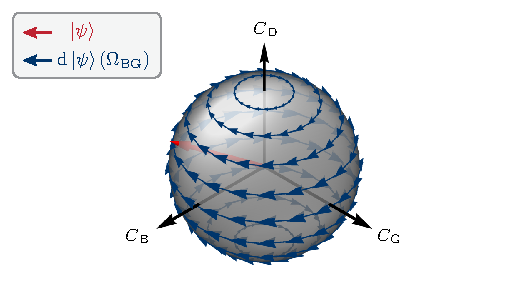
\includegraphics[scale=1.5]{qmjump/knowledge_sphere}
\par\end{centering}
\caption[Geometrical representation of a qutrit state with real coefficients:\textbf{
$\mathbb{\mathbb{R}}$}-qutrit sphere]{\label{fig:R-qutrit-sphere-representation.}\textbf{Geometrical representation
of a qutrit state with real coefficients:} $\mathbb{\mathbb{R}}$\textbf{-qutrit
sphere. }Geometric representation of the Hilbert space of pure states
of a qutrit, $\ket{\psi}=\cbn\B+\cgn\G+\cdn\D$, with real-valued
coefficients, notably isomorphic to the special orthogonal group $SO\left(3\right)$.
Overlaid vector field represents the infinitesimal state change, $\mathrm{d}\ket{\psi}$,
due to the Rabi drive $\Omega_{{\rm BG}}.$}
\end{figure}


\paragraph{Measurement-backaction  force steers atom towards $\D$. }

Although there is no Rabi drive or measurement directly applied to
the Dark level, conditioned on not detecting a click, according to
Eq.~(\ref{eq:Cdn}), a force is nonetheless exerted by the B-level
monitoring that steers the atom toward the Dark level. Specifically,
the rate of change of the D level amplitude, $\ddt\cdn$, is given
by an anti-damping term with a state-dependent rate proportional to
the B level population, $\cbn\left(t\right)^{2}$, and measurement
rate, $\gamma_{{\rm B}}$. Solving Eq.~(\ref{eq:Cdn}), one finds
\begin{equation}
\cdn\left(t\right)=\cdn\left(0\right)\exp\left(\int_{0}^{t}\mathrm{d}t'\frac{1}{2}\gamma_{{\rm B}}\cbn\left(t\right)^{2}\right)\,.\label{eq:Cdsol}
\end{equation}
In this sense, the renormalization of the conditional state amounts
to a (non-unitary) measurement-backaction force on $\D$, which is
linked to the population of $\B.$ To explicitly solve Eq.~(\ref{eq:Cdsol}),
we need to solve the remaining equations, Eqs.~(\ref{eq:Cbn}) and
(\ref{eq:Cgn}). 

\paragraph{Adiabatic elimination of the Bright state dynamics.}

Because Eq.~(\ref{eq:Cbn}) is non-linear, we consider the B level
dynamics and their adiabatic elimination with greater care. Eq.~(\ref{eq:Cbn}),
contains both a damping, $-\half\gamma_{{\rm B}}\cbn$, and an anti-damping,
$\frac{1}{2}\gamma_{{\rm B}}\cbn{}^{3}$, term. These cancel out perfectly
only if the atom is either entirely in $\B$, $\cbn=\pm1$, or not
at all in $\B$, $\cbn=0$; otherwise, $\left|\cbn\right|<1$, the
damping dominates, steering $\cbn$ in the direction of zero. In the
extreme case, where $\Omega_{{\rm BG}}=0$, one can explicitly solve
the B level dynamics, $\cbn\left(t\right)^{2}=\left[1+\left(\cbn\left(0\right)^{-2}-1\right)\exp\left(\gamma_{{\rm B}}t\right)\right]^{-1},$
which for small initial populations, $\cbn\left(0\right)^{2}\ll1$
rapidly decays to a stable zero equilibrium at a rate $\frac{1}{2}\gamma_{{\rm B}}$,
$\cbn\left(t\right)\approx\cbn\left(0\right)\exp\left(-\frac{1}{2}\gamma_{{\rm B}}t\right)$.
Since $\gamma_{{\rm B}}$ is the fastest timescale in the problem
and the B dynamics are convergent, we can adiabatically eliminate
$\cbn$ by setting $\ddt\cbn\left(t\right)=0$; solving the cubic
equation, one finds three solution branches,
\begin{equation}
\cbnb\left(t\right)=\begin{cases}
-1-\frac{\Obg}{2\gamma_{{\rm B}}}\cgn\left(t\right)+\mathcal{O}\left(\left(\Obg/\gamma_{{\rm B}}\right)^{2}\right)\\
1-\frac{\Obg}{2\gamma_{{\rm B}}}\cgn\left(t\right)+\mathcal{O}\left(\left(\Obg/\gamma_{{\rm B}}\right)^{2}\right)\\
\frac{\Obg}{\gamma_{{\rm B}}}\cgn\left(t\right)+\mathcal{O}\left(\left(\Obg/\gamma_{{\rm B}}\right)^{3}\right)\,.
\end{cases}\label{eq:Cb-bar}
\end{equation}
Operating the three-level atom in the limit where the $\B$ level
is never appreciably populated, we employ the third solution branch,
$\cbnb\left(t\right)=\frac{\Obg}{\gamma_{{\rm B}}}\cgn\left(t\right)$,
in Eq.~(\ref{eq:Cgn}) to find the effective equation of motion for
the G level dynamics, 
\begin{equation}
\ddt\cgn\left(t\right)=-\tau_{\mathrm{BG}}^{-1}\left[1-\cgn\left(t\right)^{2}\right]\cgn\left(t\right),\label{eq:ddtCGn}
\end{equation}
which are now completely decoupled from the other levels. In Eq.~(\ref{eq:ddtCGn}),
we identify a damping and an anti-damping term with a constant and
G-population dependent, $\cgn^{2}$, rate, respectively. The scale
of both terms is given by the parameter $\tau_{\mathrm{BG}}^{-1}=\Omega_{{\rm BG}}^{2}/2\gamma_{\mathrm{B}}$,
which is the expected rate of clicks when the atom is in $\G$. By
eliminating the B level, we have obtained an explicit relation for
the effective monitoring of the G level, which occurs at a rate $\tau_{{\rm BG}}^{-1}$,
which can also be interpreted as the quantum Zeno rate \citep{Misra1977,Gambetta2008-qm-traj,Matsuzaki2010,Vijay2011,Slichter2016-T1vsNbar,Harrington2017,Hacohen-Gourgy2018}.
The numerator $\Obg^{2}$ is proportional to the population transfer
rate from $\G$ to $\B$ while the denominator $\gamma_{{\rm B}}$
gives the rate of projection from $\B$ to $\G$. Solving Eq.~(\ref{eq:ddtCGn})
and substituting its solution in Eq.~(\ref{eq:Cdsol}), one finds
\begin{figure}
\begin{centering}
\includegraphics[scale=1.5]{qmjump/knowledge_img1}
\par\end{centering}
\caption[Adiabatic solution for the no-click GD manifold trajectory of a superposition
state measured with $\Odg=0$]{\textbf{\label{fig:3:adiabatic-sol}Adiabatic solution for the no-click
GD manifold trajectory of a superposition state measured with }$\Odg=0$\textbf{.
}Adiabatic-approximation (solid lines) and numerical (dashed lines)
solution for the partial tomogram of the GD manifold of the no-click
quantum trajectory of an initial superposition state $\ket{\psi\left(0\right)}=\mathcal{N}\left(\G+\epsilon\D\right)$,
where $\epsilon=0.1$ and $\mathcal{N}=\left(1+\epsilon^{2}\right)^{-1/2}$.
The Bright Rabi drive is $\Obg=0.1$, in units of the decay rate $\gamma_{{\rm B}}$.
Time axis scaled in units of $\tau_{\mathrm{BG}}=\left(\Obg^{2}/\gamma_{{\rm BG}}\right)^{-1}.$}
\end{figure}
\begin{align}
\cgn\left(t\right)^{2}= & \frac{p_{{\rm G}}}{p_{{\rm G}}+\left(1-p_{{\rm G}}\right)e^{2t/\tau_{{\rm BG}}}}\,,\label{eq:Cgnoclicksol}\\
\cdn\left(t\right)^{2}= & \frac{p_{{\rm D}}e^{t/\tau_{{\rm BG}}}}{p_{{\rm D}}+\left(1-p_{{\rm D}}\right)e^{2t/\tau_{{\rm BG}}}}\,,\label{eq:CdNoClickSol}
\end{align}
where $p_{{\rm G}}\equiv\cgn\left(0\right)^{2}$ and $p_{{\rm D}}\equiv\cdn\left(0\right)^{2}$
are the initial conditions. Note, for $p_{{\rm D}}=0$, the above
solution for $\cdn$ is always zero. The evolution of the GD Bloch
vector conditioned on no clicks for the initial state $\ket{\psi\left(0\right)}=\mathcal{N}\left(\G+\epsilon\D\right)$
is obtained by substituting Eq.~(\ref{eq:Cgnoclicksol}) and (\ref{eq:CdNoClickSol})
in Eqs.~(\ref{eqn:Z})-(\ref{eqn:Y}), 
\begin{align}
{\rm Z}_{{\rm GD}}(t) & ={\rm tanh}\left[t/\tau_{{\rm BG}}+\mathrm{arctanh}\left[{\rm Z}_{{\rm GD}}(0)\right]\right],\label{eq:Zgd-Adi}\\
{\rm X}_{{\rm GD}}(t) & ={\rm sech}\left[t/\tau_{{\rm BG}}+\mathrm{arctanh}\left[{\rm Z}_{{\rm GD}}(0)\right]\right],\\
{\rm Y}_{{\rm GD}}(t) & =0.\label{eq:Ygd-Adi}
\end{align}
We note that a few results of this subsection, especially Eqs.~(\ref{eq:Zgd-Adi})-(\ref{eq:Ygd-Adi}),
bear resemblance to results from Sec.~\ref{sec:thry:3lvl-atom-simple-log},
yet we stress that  the two situations are fundamentally distinct,
and the resemblance must be considered with care. For instance, we
note that the mid-flight time $\Delta t_{\mathrm{mid}}$ cannot be
recovered from the simpler situation considered here, where no quantum
jumps occur and there is no competition between unitary dynamics due
to $\Omega_{{\rm DG}}$ and the measurement. 

In Fig.~\ref{fig:3:adiabatic-sol}a, we plot the adiabatic-approximation
solution to the non-linear Schrödinger evolution, Eq.~(\ref{eq:NL-SSe-Cond-3}),
for the GD manifold Bloch vector conditioned on no clicks, Eqs.~(\ref{eq:Zgd-Adi})-(\ref{eq:Ygd-Adi}),
obtained in the limit $\Obg\ll\gamma_{B}$. Overlaid (dashed lines)
is the corresponding numerically calculated solution to Eq.~(\ref{eq:NL-SSe-Cond-3}).
Even for modest separation of timescales, $\Obg/\gamma_{{\rm B}}=0.1$
in the plot, the two solutions appear nearly indistinguishable. The
initial atom state, $\epsilon=0.1$, is gradually projected to $\D$
on a timescale given by $\tau_{{\rm BG}}$ and evolves in a characteristically
non-unitary manner. Notably, the state remains pure at all times,
and in the limit $t\gg\tau_{{\rm BG}}$ remains essentially in $\D$,
indefinitely. Importantly, for times $t$ on the other of $\tau_{{\rm BG}}$,
the projection can (but need not) be interrupted by the detection
of a click, which would project the state to $\G$, and occurs with
total probability $\approx1-\epsilon^{2}$. 
\begin{figure}
\begin{centering}
\includegraphics[scale=1.4]{qmjump/knowledge_img2}
\par\end{centering}
\caption[Geometrical representation of the no-click measurement-backaction
force for $\Obg=0$]{\textbf{\label{fig:Knowledge-driven-force-in-1}Geometrical representation
of the no-click measurement-backaction  force for $\Obg=0$.} Shown
are two projections of $\mathbb{\mathbb{\mathbb{R}}}$-qutrit sphere
overlaid with the measurement-force vector field, $\frac{\mathrm{d}}{\mathrm{d}t}\ket{\psi_{I=0}}$,
due to the monitoring of the B level with $\Obg=0$. Color of density
plot indicates the relative magnitude of the change, $\mathrm{Norm}\left[\frac{\mathrm{d}}{\mathrm{d}t}\ket{\psi_{I=0}}\right]$.}
\end{figure}


\paragraph{Hilbert space representation of the measurement dynamics.}

It is useful to consider a geometric representation of the measurement
dynamics and in particular of the non-linear measurement-backaction
force. For simplicity, first consider the measurement force due only
to the monitoring of the B level, in the absence of the Bright Rabi
drive, $\Obg=0$. This  force can be represented as a vector field
on the surface of the $\mathbb{R}$-qutrit sphere, see Fig.~\ref{fig:Knowledge-driven-force-in-1}.
The vector field is calculated from Eqs.~(\ref{eq:Zgd-Adi})-(\ref{eq:Ygd-Adi})
for the change in the state conditioned on detecting no clicks, 
\begin{equation}
\frac{\mathrm{d}}{\mathrm{d}t}\ket{\psi_{I=0}}=\frac{1}{2}\gamma_{{\rm B}}\cbn{}^{2}\begin{pmatrix}\cbn-1\\
\cgn\\
\cdn
\end{pmatrix}\,.\label{eq:ddtPsiI-vec}
\end{equation}
The colormap in Fig.~\ref{fig:Knowledge-driven-force-in-1} depicts
the relative magnitude of the change, $\mathrm{Norm}\left[\frac{\mathrm{d}}{\mathrm{d}t}\ket{\psi_{I=0}}\right],$
which we note is only zero in two special cases: i) when the atom
is $\pm\B$, corresponding to the points $\left(\pm1,0,0\right),$
and ii) when the atom is in a\emph{ }state involving exclusively $\G$
and $\D$ but not $\B$. The latter is special in that it corresponds
to an entire manifold of states, the GD equatorial circle, which can
be visually recognized in Fig.~\ref{fig:Knowledge-driven-force-in-1}
as the dark vertical stripe at the center of the left panel and the
dark circular perimeter of the disk in the right panel. All other
states, not covered under the latter two cases, are superpositions
involving $\B$. From the vector field plot, it is evident that these
states are guided by the force away from the $\B$ poles and toward
the GD equator. It is precisely this feature of the measurement force
that results in the gradual projection of the state conditioned on
no clicks — it is the unavoidable disturbance of the atom due to the
information-gain of the no-click measurement outcomes, which lead
the observer to gradually learn that the atom is not in $\D$, thus
resulting in the increased likelihood that it is in $\G$ or $\D$.
This dynamics embody the message of the Chapter~\ref{chap:Quantum-Trajectory-Theory}
epigraph, ``In quantum physics you don't see what you get, you get
what you see.''

\begin{figure}
\begin{centering}
\includegraphics[scale=1.4]{qmjump/knowledge_img3}
\par\end{centering}
\caption[Geometrical representation of the measurement-backaction force and
a no-click trajectory with $\Obg=0.1\gamma_{{\rm B}}$]{\textbf{\label{fig:Knowledge-driven-force-in-2}Geometrical representation
of the measurement-backaction force and a no-click trajectory with
$\Obg=0.1\gamma_{{\rm B}}$.}  Two projections of the $\mathbb{\mathbb{\mathbb{R}}}$-qutrit
sphere overlaid with the measurement-force vector field $\frac{\mathrm{d}}{\mathrm{d}t}\ket{\psi_{I=0}}$
(blue arrows) and the path of the quantum trajectory from Fig.~(\ref{fig:3:adiabatic-sol})
(red arrows), depicting the gradual projection of a superposition
state to $\D$ conditioned on no clicks. Density plot indicates relative
field magnitude, $\mathrm{Norm}\left[\frac{\mathrm{d}}{\mathrm{d}t}\ket{\psi_{I=0}}\right]$.}
\end{figure}

In Fig.~\ref{fig:Knowledge-driven-force-in-2}, we plot the measurement
vector field in the presence of the Bright Rabi drive $\Omega_{\mathrm{BG}}$,
\begin{equation}
\frac{\mathrm{d}}{\mathrm{d}t}\ket{\psi_{I=0}}=\frac{1}{2}\gamma_{{\rm B}}\cbn{}^{2}\begin{pmatrix}\cbn-1\\
\cgn\\
\cdn
\end{pmatrix}+\frac{1}{2}\Obg\begin{pmatrix}\cgn\\
-\cbn\\
0
\end{pmatrix}\,,\label{eq:ddtPsiI-vec-1}
\end{equation}
with $\Obg=0.1\gamma_{{\rm B}}$. The Bright Rabi drive, visually
represented on the $\mathbb{R}$-qutrit sphere in Fig.~\ref{fig:R-qutrit-sphere-representation.},
perturbs the measurement field, shown in Fig.~\ref{fig:Knowledge-driven-force-in-1},
by linking the B and G levels and lifting the degeneracy of the measurement,
represented in GD equator. Visually, this is evident in the tilt of
the vertical dark stripe in the center of the left-panel colormap.
In the right panel, it is also evident that $\B$ is no longer an
equilibrium point; the equilibrium has been shifted in the direction
of $\G$ by an amount proportional $\Obg/\gamma_{{\rm B}},$ see Eq.~(\ref{eq:Cb-bar}),
and made metastable. The red arrows depict the path of the quantum
trajectory in Hilbert of the gradual projection of an initial superposition
state of $\G$ and $\D$, for the same parameters as employed in Fig.~(\ref{fig:3:adiabatic-sol}),
where $\epsilon=0.1$. Initially, the state is quickly steered in
the direction of $\B$ by the force of $\Obg$. However, as the state
moves in the direction of $\B$, the motion is quickly opposed by
the no-click measurement-backaction force, which grows larger in amplitude
in this direction. The two forces do not precisely cancel each other
out, because of the slight mismatch in angles. The net force, albeit
small, steers the atom towards the GD equator and with a slight tilt
toward $\D$. The opposition of the $\Obg$ drive and the measurement
back-action ``trap'' the state in the ridge where the two forces
nearly cancel each other out, the nearly vertical dark stripe in the
left panel, and the small angular mismatch slowly carries the state
in the direction of $\D$, an equilibirum point, where all forces
are zero.


\subsection{Incoherent Bright drive and Dark drive off\label{subsec:Incoherent-Bright-drive}}

In this section, we consider the case of quantum jumps in the three-level
atom subject to photodetection and an incoherent Bright drive, rather
than a Rabi one, see Sec.~\ref{sec:thry:3lvl-atom-simple-log}. The
situation analyzed in this section is somewhat more analogous to the
cQED experiment where the Bright Rabi drive consists of a bi-chromatic
tone that unconditionally addresses the BG transition, independent
of the population of the readout cavity, necessitated by the  dispersive
pull of the readout cavity on the BG frequency. The bi-chromatic drive
effectively acts as an incoherent drive. The incoherent Bright drive
photodetection theory presented here sheds some further light on the
dynamics of the quantum jump from $\G$ to $\D$. Features such as
the non-zero coherence, $X_{{\rm GD}}$, and in the limit $\deltatcatch\gg\Delta t_{{\rm mid}}$
are discussed.\footnote{The following derivation is due to H.J. Carmichael and R. Gutierrez-Jauregui.}

Replacing the coherent Rabi drive $\Omega_{{\rm BG}}$ by an incoherent
drive $\Gamma_{{\rm BG}}$ in  the master equation of the three-level
atom in the interaction picture, Eq.~(\ref{eq:PhotonLindblad}) becomes
\begin{equation}
\frac{\mathrm{d}\rho}{\mathrm{d}t}=(i\hbar)^{-1}[\hat{H}_{{\rm drive}},\rho]+\Gamma_{{\rm BG}}{\cal D}\left[\kb{\rm B}{\rm G}\right]\rho+(\gamma_{{\rm B}}+\Gamma_{{\rm BG}}){\cal D}\left[\kb{\rm G}{\rm B}\right]\rho+\gamma_{{\rm D}}{\cal D}\left[\kb{\rm G}{\rm D}\right]\rho,
\end{equation}
and Eq.~(\ref{eq:ClickHeff}) becomes
\begin{equation}
\hat{H}_{{\rm drive}}=i\hbar\frac{\Omega_{{\rm DG}}}{2}\big(\kb{\rm D}{\rm G}-\kb{\rm G}{\rm D}\big).
\end{equation}
The strong-monitoring assumption, $\tau_{{\rm BG}}^{-1}\ll\gamma_{{\rm B}}$,
is also carried over from Sec.~\ref{sec:thry:3lvl-atom-simple-log}
by assuming $\Gamma_{{\rm BG}}\ll\gamma_{{\rm B}}$, i.e., the time
between clicks in fluorescence is essentially the same as the time
separating photon absorptions from the incoherent drive, as absorption
is rapidly followed by fluorescence ($\gamma_{{\rm B}}+\Gamma_{{\rm BG}}\gg\Gamma_{{\rm BG}}$).
This brings a useful simplification, since, following each reset to
$\G$, the unnormalized state evolves in the GD-subspace, 
\begin{equation}
i\hbar\frac{\mathrm{d}\ket{\tilde{\psi}}}{\mathrm{d}\Delta t_{{\rm catch}}}=\left(\hat{H}_{{\rm drive}}-i\hbar\frac{\Gamma_{{\rm BG}}}{2}\kb{\rm G}{\rm G}-i\hbar\frac{\gamma_{{\rm D}}}{2}\kb{\rm D}{\rm D}\right)\ket{\tilde{\psi}},
\end{equation}
thus replacing Eqs.~(\ref{eqn:3x3_system}) and (\ref{eqn:W_DG_equation_coherent})
by the simpler $2\times2$ system 
\begin{equation}
\frac{\mathrm{d}}{\mathrm{d}\Delta t_{{\rm catch}}}\begin{pmatrix}\cg\\
\cd
\end{pmatrix}=\frac{1}{2}\left(\begin{matrix}-\Gamma_{{\rm BG}} & -\Omega_{{\rm DG}}\\
\Omega_{{\rm DG}} & -\gamma_{{\rm D}}
\end{matrix}\right)\begin{pmatrix}\cg\\
\cd
\end{pmatrix},
\end{equation}
and, in the limit $\gamma_{{\rm D}}\ll\Gamma_{{\rm BG}}$, the equation
of motion for $W_{{\rm DG}}$, defined in Eq.~(\ref{eqn:W_DG_definition}),
is
\begin{equation}
\frac{\mathrm{d}W_{{\rm DG}}}{\mathrm{d}\Delta t_{{\rm catch}}}=\frac{\Gamma_{{\rm BG}}}{2}W_{{\rm DG}}+\frac{\Omega_{{\rm DG}}}{2}(1+W_{{\rm DG}}^{2}),\label{eqn:W_DG_equation_incoherent}
\end{equation}
with solution, for $W_{{\rm DG}}(0)=0$, 
\begin{equation}
W_{{\rm DG}}(\Delta t_{{\rm catch}})=\frac{\exp\left[(V-V^{-1})\Omega_{{\rm DG}}\Delta t_{{\rm catch}}/2\right]-1}{V-V^{-1}\exp\left[(V-V^{-1})\Omega_{{\rm DG}}\Delta t_{{\rm catch}}/2\right]},\label{eqn:W_DG_incoherent}
\end{equation}
where 
\begin{equation}
V=\frac{1}{2}\frac{\Gamma_{{\rm BG}}}{\Omega_{{\rm DG}}}+\sqrt{\frac{1}{4}\left(\frac{\Gamma_{{\rm BG}}}{\Omega_{{\rm DG}}}\right)^{2}-1}.
\end{equation}
In Ref.~\citet{Ruskov2007}, a general form of the Bloch vector equations
for arbitrary amplitude of the Rabi drive was found. Inversion of
the condition $W_{{\rm DG}}(\Delta t_{{\rm mid}})=1$ gives the characteristic
time scale 
\begin{equation}
\Delta t_{{\rm mid}}=2\left[(V-V^{-1})\Omega_{{\rm DG}}\right]^{-1}\ln\left(\frac{V+1}{V^{-1}+1}\right).\label{eqn:t_mid_incoherent}
\end{equation}
Although Eqs.~(\ref{eqn:W_DG_incoherent}) and (\ref{eqn:t_mid_incoherent})
replace Eqs.~(\ref{eq:WDG-coh}) and (\ref{eq:t_mid_coherent}),
under strong monitoring, $\Gamma_{{\rm BG}}\gg\Omega_{{\rm DG}}$,
they revert to the latter with the substitution $\Omega_{{\rm BG}}^{2}/2\gamma_{{\rm B}}\to\Gamma_{{\rm BG}}/2$,;
in this way, Eqs.~(\ref{eqn:Z})–(\ref{eqn:Y}) are recovered with
the same substitution. More generally, $W_{{\rm DG}}(\Delta t_{{\rm catch}})$
goes to infinity at finite $\Delta t_{{\rm catch}}$, changes sign,
and returns from infinity to settle on the steady value $W_{{\rm DG}}(\infty)=-V$.
The singular behavior marks a trajectory passing through the north
pole of Bloch sphere. It yields the long-time solution 
\begin{equation}
{\rm Z}_{{\rm GD}}(\infty)=\sqrt{1-4\left(\frac{\Omega_{{\rm DG}}}{\Gamma_{{\rm BG}}}\right)^{2}},\qquad{\rm X}_{{\rm GD}}(\infty)=-2\frac{\Omega_{{\rm DG}}}{\Gamma_{{\rm BG}}},\qquad{\rm Y}_{{\rm GD}}(\infty)=0,\label{eq:ZGDXGD-long-term}
\end{equation}
in contrast to the perfect jump of Eqs.~(\ref{eqn:Z_approx})–(\ref{eqn:Y_approx}).
The long-term coherence and lower-than-one value of Z were observed
in the experiments, see Fig.~\ref{fig:catch}b. They can be understood
as the equilibrium point of the coherent Rabi drive $\Omega_{{\rm DG}}$
attempting to rotate the state from $\D$ back to $\G$ perfectly
balanced against the measurement-backaction force of the no-click
measurement steering the atom toward $\D$, recall discussion of the
measurement vector field, see Figs.~\ref{fig:Knowledge-driven-force-in-1}
and~\ref{fig:Knowledge-driven-force-in-2}. 

\paragraph{\textit{\emph{Dark drive off.}}}

Turing the Dark drive off shortly after a click demonstrates the connection
between the flight of a quantum jump and a projective measurement.
From the point of view of the trajectory equations, the only change
is the setting of $\Omega_{{\rm DG}}$ to zero at time $\Delta t_{{\rm on}}$
on the right-hand side of Eqs.~(\ref{eqn:W_DG_equation_coherent})
and (\ref{eqn:W_DG_equation_incoherent}). Subsequently, $W_{{\rm DG}}(\Delta t_{{\rm catch}})$
continues its exponential growth at rate $\Omega_{{\rm BG}}^{2}/2\gamma_{B}$
{[}Eq.~(\ref{eqn:W_DG_equation_coherent}){]} or $\Gamma_{{\rm BG}}/2$
{[}Eq.~(\ref{eqn:W_DG_equation_incoherent}){]}. Equations (\ref{eqn:Z})–(\ref{eqn:Y})
for the GD Bloch components still hold, but now with 
\begin{equation}
\Delta t_{{\rm mid}}=\left(\frac{\Omega_{{\rm BG}}^{2}}{2\gamma_{B}},\frac{\Gamma_{{\rm BG}}}{2}\right)^{-1}\ln\big[W_{{\rm DG}}^{-2}(\Delta t_{{\rm on}})\big].
\end{equation}
which can provide an estimate of $\Delta t'_{\mathrm{mid}}$, specifying
the time at which $Z_{\mathrm{GD}}=0$.

The evolution during $\Delta t_{\mathrm{off}}$, in the absence of
$\Omega_{\mathrm{DG}}$, in effect realizes a projective measurement
of whether the state of the atom is $\G$ or $|{\rm D}\rangle$, similar
to the one analyzed in Sec.~\ref{subsec:Knowledge-driven-force-in},
where the normalized state at $\Delta t_{{\rm on}}$ is 
\begin{equation}
\frac{|\psi(\Delta t_{{\rm on}})\rangle}{\sqrt{\mathcal{N}(\Delta t_{{\rm on}})}}=\frac{\cg(\Delta t_{{\rm on}})\G+\cd(\Delta t_{{\rm on}})\D}{\sqrt{\mathcal{N}(\Delta t_{{\rm on}})}},\label{eqn:initial_state}
\end{equation}
with $\mathcal{N}(\Delta t_{{\rm on}})=\cg^{2}(\Delta t_{{\rm on}})+\cd^{2}(\Delta t_{{\rm on}})$
the probability for the jump to reach $\Delta t_{{\rm catch}}=\Delta t_{{\rm on}}$
after a click reset to $\G$ at $\Delta t_{{\rm catch}}=0$. The probability
for the jump to continue to $\Delta t_{{\rm catch}}>\Delta t_{{\rm on}}$
(given $\Delta t_{{\rm on}}$ is reached) is then 
\begin{equation}
\frac{\mathcal{N}(\Delta t_{{\rm catch}})}{\mathcal{N}(\Delta t_{{\rm on}})}=\frac{C_{{\rm D}}^{2}(\Delta t_{{\rm on}})}{\mathcal{N}(\Delta t_{{\rm on}})}+\frac{C_{{\rm G}}^{2}(\Delta t_{{\rm on}})}{\mathcal{N}(\Delta t_{{\rm on}})}\exp\left[-\left(\frac{\Omega_{{\rm BG}}^{2}}{\gamma_{{\rm B}}},\Gamma_{{\rm BG}}\right)\Delta t_{{\rm catch}}\right].\label{eq:completion-prob}
\end{equation}


\paragraph{Completed and aborted evolutions of the jump transition.}

In this simple model, the probability for the trajectory to complete
— for the measurement to yield the result $|{\rm D}\rangle$ — is
obtained in the limit $\Delta t_{\mathrm{catch}}\rightarrow\infty$,
and, as expected, is equal to the probability to occupy the state
$|{\rm D}\rangle$ at time $\Delta t_{{\rm on}}$; i.e., the completion
probability is $P_{\mathrm{D}}(\Delta t_{{\rm on}})=C_{{\rm D}}^{2}(\Delta t_{{\rm on}})/{{\rm Norm}(\Delta t_{{\rm on}})}$.
It is helpful to illustrate this idea with an example. Consider the
catch experiment of Fig.~\ref{fig:catch}b in the absence of the
Dark Rabi drive, $\Omega_{\mathrm{DG}}$. From $Z_{\mathrm{GD}}$,
we can estimate that out of all the trajectories that pass though
the $\Delta t_{{\rm on}}$ mark approximately $P_{\mathrm{D}}(\Delta t_{{\rm on}})=(1+Z_{\mathrm{GD}}(\Delta t_{{\rm on}}))/2\approx8\%$
fully complete without an interruption. On the other hand, for those
that pass the $\Delta t'_{\mathrm{mid}}$ mark, approximately 50\%
complete. It follows from Eq.~(\ref{eq:completion-prob}), that the
probability of the evolution to complete increases the further along
the trajectory is. Although some of the jump evolutions abort at random,
importantly, every single jump evolution that completes, and is thus
recorded as a jump, follows \textit{not} a random but an identical
path in Hilbert space, i.e., a deterministic one. This path (of \textit{any}
jump) is determined by Eq.~(\ref{eqn:W_DG_incoherent}), or, in the
simpler model, by the Eqs.~(\ref{eqn:Z_approx})-(\ref{eqn:Y_approx})
for the components of the GD Bloch vector.

\section{Heterodyne monitoring of readout cavity coupled to three-level atom\label{sec:Heterodyne-monitoring-of}}

\subsection{Description of cQED experiment \label{subsec:Description-of-cQED}}

In Chapter 1, we described the cQED experiment  involving a superconducting
atom with the necessary V-shape level structure (see Fig.~\ref{fig:setup}a
or Sec.~\ref{sec:circuit-design}) subject to heterodyne monitoring
of $\B$ by means a dispersively coupled readout cavity. The three-level
atom is formed form two heavily hybridized transmon modes, which are
coupled by means of a cross-Kerr interaction to the readout cavity
in an asymmetric way, $\chi_{\mathrm{BC}}\gg\chi_{\mathrm{DC}}$.
In the following, we present the quantum trajectory description of
the heterodyne monitoring, including imperfections.

\paragraph{System Hamiltonian. }

In the lab frame, the Hamiltonian of the system is, see also Sec.~\ref{sec:circuit-design},
\begin{equation}
\hat{H}_{{\rm lab}}=\hat{H}_{0}+\hat{H}_{I}+\hat{H}_{d}\left(t\right)\,,
\end{equation}
where the Hamiltonian of the uncoupled three-level atom and cavity,
is 
\begin{equation}
\hat{H}_{0}=\hbar\omega_{{\rm DG}}\kb{\rm D}{\rm D}+\hbar\omega_{{\rm BG}}\kb{\rm B}{\rm B}+\hbar\omega_{C}\hat{c}^{\dagger}\hat{c}\,,
\end{equation}
where $\omega_{{\rm DG}}$, $\omega_{{\rm BG}}$, $\omega_{{\rm C}}$
are the Dark, Bright, and cavity mode frequency, respectively, $\hat{c}$
is the cavity amplitude operator, the atom-cavity interaction Hamiltonian
is 
\begin{equation}
\hat{H}_{I}=\hat{c}^{\dagger}\hat{c}\left[\hbar\chi_{{\rm B}}\kb{\rm B}{\rm B}+\hbar\chi_{{\rm D}}\kb{\rm D}{\rm D}\right]\:,
\end{equation}
where the shift of the cavity frequency conditioned on $\B$ ($\D$)
is $\chi_{{\rm B}}$ ($\chi_{{\rm D}}$), and the Hamiltonian of the
atom Rabi drives and readout probe tone is
\begin{align}
\hat{H}_{d}\left(t\right)= & -\frac{i\hbar}{2}\left[\kappa\sqrt{\bar{n}}\hat{c}e^{i\left(\omega_{{\rm C}}+\Delta_{{\rm R}}\right)t}+\Omega_{{\rm DG}}^{*}e^{i\left(\omega_{{\rm DG}}+\Delta_{{\rm DG}}\right)t}\kb{\rm G}{\rm D}\right.\nonumber \\
 & \left.+\Omega_{{\rm B0}}^{*}e^{i\omega_{{\rm BG}}t}\kb{\rm G}{\rm B}+\Omega_{{\rm B1}}^{*}e^{i\left(\omega_{{\rm BG}}+\Delta_{{\rm B1}}\right)t}\kb{\rm G}{\rm B}+\mathrm{H.c.}\right]\,,
\end{align}
where $\bar{n}$ is the steady state number of photons in the cavity
when driven resonantly, $\Delta_{{\rm R}}$, $\Delta_{{\rm DG}},$
and $\Delta_{{\rm B1}}$ are the drive detunings from the bare mode
frequencies. The first Bright Rabi tone, $\Omega_{{\rm B0}}$, addresses
the Bright transition when the cavity is unpopulated, while the second
tone, $\Omega_{{\rm B0}}$, addresses the BG transition  when the
cavity is populated, see frequency spectrum in Fig.~\ref{fig:setup}c.
Moving to the rotating frame at the drive frequencies, defined by
the ket transformation $\ket{\psi(t)}=U(t)\ket{\psi_{\mathrm{lab}}(t)}$,
where $U(t)=\exp\left(u\left(t\right)/i\hbar\right)$ and $u(t)=\hbar t\left[\left(\omega_{{\rm C}}+\Delta_{{\rm R}}\right)a^{\dagger}a+\omega_{{\rm BG}}\ket{\rm B}\bra{\rm B}+\left(\omega_{{\rm DG}}+\Delta_{{\rm DG}}\right)\ket{\rm D}\bra{\rm D}\right]$,
the Hamiltonian in the rotating frame is
\begin{equation}
\hat{H}\left(t\right)=\hat{H}_{{\rm R}}+\hat{H}_{{\rm drive}}\left(t\right)\,,
\end{equation}
where $\hat{H}_{\mathrm{R}}$ is a time-independent Hamiltonian,
\begin{equation}
\hat{H}_{{\rm R}}=-\hbar\Delta_{{\rm R}}\hat{c}^{\dagger}\hat{c}+i\hbar\frac{\kappa}{2}\sqrt{\bar{n}}(\hat{c}^{\dagger}-\hat{c})+\hbar\big(\chi_{{\rm B}}\kb{\rm B}{\rm B}+\chi_{{\rm D}}\kb{\rm D}{\rm D}\big)\hat{c}^{\dagger}\hat{c},
\end{equation}
and $\hat{H}_{{\rm drive}}$ is the time-dependent Hamiltonian of
the atom Rabi drives, 
\begin{equation}
\hat{H}_{{\rm drive}}\left(t\right)=i\hbar\left[\frac{\Omega_{{\rm BG}}(t)}{2}\kb{\rm B}{\rm G}-\frac{\Omega_{{\rm BG}}^{*}(t)}{2}\kb{\rm G}{\rm B}\right]+i\hbar\frac{\Omega_{{\rm DG}}}{2}\left(\kb{\rm D}{\rm G}-\kb{\rm G}{\rm D}\right).
\end{equation}
The bi-chromatic drive, which unselectively addresses the BG transition,
$\Omega_{{\rm BG}}(t)=\Omega_{{\rm B}0}+\Omega_{{\rm B}1}\exp(-i\Delta_{{\rm B}1}t)$
replaces the Rabi drive $\Omega_{{\rm BG}}$ of Eq.~(\ref{eq:drive_coherent_fluorescence}).

\paragraph{Measurement record.}

The readout cavity input-output coupling is given by the jump operator
$\sqrt{\kappa}\hat{c}$. It follows from Eq.~(\ref{eq:dJimperf:het})
that the heterodyne measurement-record increment is
\begin{equation}
\mathrm{d}J_{\mathrm{het}}\left(t\right)=\sqrt{\eta\kappa}\left\langle \hat{c}\right\rangle \left(t\right)\dt+\dZ\left(t\right)\,,\label{eq:Record}
\end{equation}
where $\dZ$ is a complex Wiener increment, see discussion below Eq.~(\ref{eq:Jhet-perfect}),
and $\eta$ is the quantum efficiency of the readout and amplification
chain. The record, $\mathrm{d}J_{\mathrm{het}}\left(t\right)$, is
scaled — to units of (readout cavity photon number)$^{1/2}$ — and
filtered to generate the simulated quadratures $I_{{\rm rec}}$ and
$Q_{{\rm rec}}$ of the measurement record: 
\begin{eqnarray}
dI_{{\rm rec}} & = & -\frac{\kappa_{{\rm filter}}}{2}\left[I_{{\rm rec}}dt-\left(\eta\frac{\kappa}{2}\right)^{-1/2}{\rm Re}(\mathrm{d}J_{\mathrm{het}})\right],\label{eqn:simulated_I_int}\\
dQ_{{\rm rec}} & = & -\frac{\kappa_{{\rm filter}}}{2}\left[Q_{{\rm rec}}dt-\left(\eta\frac{\kappa}{2}\right)^{-1/2}{\rm Im}(\mathrm{d}J_{\mathrm{het}})\right],\label{eqn:simulated_Q_int}
\end{eqnarray}
where $\kappa_{{\rm filter}}$ is the bandwidth of the amplifier chain.
In practice, it is assured that $\kappa_{{\rm filter}}$ is the fastest
rate in the problem, $\kappa_{{\rm filter}}\gg\kappa$, so that its
effect is largely negligible.  

\subsection{Simulation of Stochastic Schrödinger equation (SSE) \label{subsec:Simulation-of-linear}}

The quantum trajectory unraveling monitors the reflected probe with
efficiency $\eta$ and accounts for residual photon loss through random
jumps. It follows that the linear stochastic Schrödinger equation
combines a continuous evolution (heterodyne readout channel), 
\begin{equation}
{\rm d}\ket{\psi\left(t\right)}=\left[\frac{1}{i\hbar}\left(\hat{H}_{{\rm drive}}+\hat{H}_{{\rm R}}-i\hbar\frac{\kappa}{2}\hat{c}^{\dagger}\hat{c}\right)\dt+\sqrt{\eta\kappa}\mathrm{d}J_{\mathrm{het}}^{*}\left(t\right)\hat{c}\right]\ket{\psi\left(t\right)},\label{eqn:SSE_continuous}
\end{equation}
with the point-like process (photon loss), 
\begin{equation}
\ket{\psi}\to\hat{c}\ket{\psi}\qquad\text{at rate}\qquad(1-\eta)\kappa\frac{\braOket{\psi}{\hat{c}^{\dagger}\hat{c}}{\psi}}{\braket{\psi}{\psi}}.
\end{equation}
Note that for perfect quantum efficiency, $\eta=1$, the rate of the
photon loss channel goes to zero. We emphasize that expectation values
are performed over the normalized state; importantly, when calculating
the measurement record increment $\mathrm{d}J_{\mathrm{het}}^{*}\left(t\right)$,
see Eq.~(\ref{eq:Record}), $\left\langle \hat{c}\right\rangle \left(t\right)=\braOket{\psi\left(t\right)}{\hat{c}}{\psi\left(t\right)}/\braket{\psi\left(t\right)}{\psi\left(t\right)}.$

\paragraph{\textit{\emph{Independently measured imperfections.}}\emph{ }}

To more realistically model the cQED experiment, we need to account
for the small experimental non-idealities associated with the device
performance; namely, the finite energy relaxation lifetime of the
levels ($T_{1}$), the finite dephasing time of the levels ($T_{2}^{*}$),
which is generally smaller than the bound imposed by the lifetime,
$T_{2}^{*}<T_{1}$, and the finite temperature of the device ($n_{{\rm th}}$).
Specifically, we supplement the stochastic Schrödinger equation by
spontaneous and thermal jumps on both the $\G$ to $\B$ and $\G$
to $\D$ transitions ($n_{{\rm th}}^{{\rm B}}$ and $n_{{\rm th}}^{{\rm D}}$)
and by pure dephasing of the ${\rm GB}$ and ${\rm GD}$ coherences
($\gamma_{{\rm B}}^{\phi}$ and $\gamma_{{\rm D}}^{\phi}$). With
these processes included, the term 
\[
-i\hbar\left\{ \left[\frac{\gamma_{{\rm B}}}{2}(n_{{\rm th}}^{{\rm B}}+1)+\gamma_{{\rm B}}^{\phi}\right]\kb{\rm B}{\rm B}+\left[\frac{\gamma_{{\rm D}}}{2}(n_{{\rm th}}^{{\rm D}}+1)+\gamma_{{\rm D}}^{\phi}\right]\kb{\rm D}{\rm D}+\frac{\gamma_{{\rm B}}n_{{\rm th}}^{{\rm B}}+\gamma_{{\rm D}}n_{{\rm th}}^{{\rm D}}}{2}|\kb{\rm G}{\rm G}\right\} 
\]
is added to the non-Hermitian Hamiltonian, $\hat{H}_{{\rm drive}}+\hat{H}_{{\rm R}}-i\hbar\frac{\kappa}{2}\hat{c}^{\dagger}\hat{c}$,
on the right-hand side of Eq.~(\ref{eqn:SSE_continuous}), with the
additional three point-processes: 
\begin{align}
|\psi\rangle\to|{\rm G}\rangle & \quad\text{at rate}\quad\gamma_{{\rm B}}(n_{{\rm th}}^{{\rm B}}+1)\frac{\langle\psi|{\rm B}\rangle\langle{\rm B}|\psi\rangle}{\langle\psi|\psi\rangle}+\gamma_{{\rm D}}(n_{{\rm th}}^{{\rm D}}+1)\frac{\langle\psi|{\rm D}\rangle\langle{\rm D}|\psi\rangle}{\langle\psi|\psi\rangle},\\
\noalign{\vskip4pt}|\psi\rangle\to|{\rm B}\rangle & \quad\text{at rate}\quad\gamma_{{\rm B}}n_{{\rm th}}^{{\rm B}}\frac{\langle\psi|{\rm G}\rangle\langle{\rm G}|\psi\rangle}{\langle\psi|\psi\rangle}+2\gamma_{{\rm B}}^{\phi}\frac{\langle\psi|{\rm B}\rangle\langle{\rm B}|\psi\rangle}{\langle\psi|\psi\rangle},\\
\noalign{\vskip4pt}|\psi\rangle\to|{\rm D}\rangle & \quad\text{at rate}\quad\gamma_{{\rm D}}n_{{\rm th}}^{{\rm D}}\frac{\langle\psi|{\rm G}\rangle\langle{\rm G}|\psi\rangle}{\langle\psi|\psi\rangle}+2\gamma_{{\rm D}}^{\phi}\frac{\langle\psi|{\rm D}\rangle\langle{\rm D}|\psi\rangle}{\langle\psi|\psi\rangle}.
\end{align}
In the simulation, the parameters $\gamma_{{\rm B,D}}$, $n_{{\rm th}}^{{\rm B,D}}$,
and $\gamma_{{\rm B,D}}^{\phi}$ are mapped to the independently measured
parameters $T_{{\rm B,D}}^{1}$, $n_{{\rm th}}^{{\rm G,D}}$, and
$T_{2{\rm R}}^{{\rm B,D}}$ listed in Table \ref{fig:T1-vs-nbar}.

\paragraph{\textit{\emph{Leakage from the }}\emph{GBD}\textit{\emph{-manifold.}}\emph{ }}

Because the three-level atom is realized from two transmon qubits,
the three-state manifold, $\left\{ \G,\B,\D\right\} $, is not strictly
closed, and transitions to higher excited states are sometimes observed.
This imperfection is modeled in the SSE simulation with the addition
of the further term 
\[
-i\hbar\left\{ \frac{\gamma_{{\rm FG}}}{2}|{\rm G}\rangle\langle{\rm G}|+\frac{\gamma_{{\rm FD}}}{2}|{\rm D}\rangle\langle{\rm D}|+\frac{\gamma_{{\rm GF}}+\gamma_{{\rm DF}}}{2}|{\rm F}\rangle\langle{\rm F}|\right\} 
\]
to the non-Hermitian Hamiltonian, and the associated additional random
jumps, 
\begin{eqnarray}
|\psi\rangle\to|{\rm F}\rangle &  & \qquad\hbox{at\ rate}\qquad\gamma_{{\rm FG}}\frac{\langle\psi|{\rm G}\rangle\langle{\rm G}|\psi\rangle}{\langle\psi|\psi\rangle}+\gamma_{{\rm FD}}\frac{\langle\psi|{\rm D}\rangle\langle{\rm D}|\psi\rangle}{\langle\psi|\psi\rangle},\\
\noalign{\vskip4pt}|\psi\rangle\to|{\rm G}\rangle &  & \qquad\hbox{at\ rate}\qquad\gamma_{{\rm GF}}\frac{\langle\psi|{\rm F}\rangle\langle{\rm F}|\psi\rangle}{\langle\psi|\psi\rangle},\\
\noalign{\vskip4pt}|\psi\rangle\to|{\rm D}\rangle &  & \qquad\hbox{at\ rate}\qquad\gamma_{{\rm DF}}\frac{\langle\psi|{\rm F}\rangle\langle{\rm F}|\psi\rangle}{\langle\psi|\psi\rangle},\label{eqn:jumps_to_F}
\end{eqnarray}
where $|{\rm F}\rangle$ models the all higher level by a single catch-all
higher excited state. The results of the simulation are presented
in Sec.~\ref{subsec:Comparison-between-theory}.


\newpage
\section*{Methods}
\subsection*{Experimental setup}

The Large Hadron Collider (LHC) is the world’s highest-energy particle accelerator and is situated approximately 100\,m underground, close to Geneva, Switzerland. The collider accelerates two counter-rotating beams of protons, guided by superconducting magnets located around a 27\,km circular tunnel, and brings them into collision at four interaction points that house large detectors. The LHCb experiment~\cite{Alves:2008zz,LHCb-DP-2014-002} is instrumented in the region covering the polar angles between 10 and 250\,mrad around the proton beam axis, in which the products from $B$-hadron decays can be efficiently captured and identified. The detector includes a high-precision tracking system with a dipole magnet, providing measurements of momentum and impact parameter (IP), defined for charged particles as the minimum distance of a track to a primary proton-proton interaction vertex (PV). Different types of charged particles are distinguished using information from two ring-imaging Cherenkov (RICH) detectors, a calorimeter and a muon system~\cite{LHCb-DP-2014-002, LHCb-DP-2014-001, LHCb-DP-2013-003,LHCb-DP-2013-001,LHCb-DP-2012-003,LHCb-DP-2012-002}. 

Since the associated data storage and analysis costs would be prohibitive, the experiment does not record all collisions. 
Only potentially interesting events, selected using real-time event filters referred to as triggers, are recorded.
% Instead, a subset of interesting events are isolated for further study using real-time event filters known as triggers. 
The LHCb trigger system has a hardware stage, based on information from the calorimeter and muon systems; followed by a software stage that uses all the information from the detector, including the tracking, to make the final selection of events to be recorded for subsequent analysis. The trigger selection algorithms are based on identifying key characteristics of $B$ hadrons and their decay products, such as high \pt final state particles, and a decay vertex that is significantly displaced from any of the PVs in the event.

For the \RK measurement, candidate events are  required to have passed a hardware trigger algorithm that selects either a high \pt muon; or an electron, hadron or photon with high transverse energy deposited in the calorimeters. The \BuKmm and \BuJpsiKmm candidates must be triggered by one of the muons, whereas \BuKee and \BuJpsiKee candidates must be triggered in one of three ways: by either one of the electrons; by the kaon from the \Bp decay; or by particles in the event that are not decay products of the \Bp candidate. In the software trigger, the tracks of the final-state particles are required to form a displaced vertex with good fit quality. A multivariate algorithm is used for the identification of displaced vertices consistent with the decay of a $B$ hadron~\cite{BBDT, LHCb-PROC-2015-018}.

\subsection*{Analysis description}

The analysis technique used to obtain the results presented in this article is essentially identical to that used to obtain the previous LHCb \RK measurement, described in Ref.~\cite{LHCb-PAPER-2019-009} and only the main analysis steps are reviewed here. 

\subsubsection*{Event selection} 

Kaon and muon candidates are identified using the output of multivariate classifiers that exploit information from the tracking system, the RICH detectors, the calorimeters and the muon chambers.
Electrons are identified by matching tracks to  particle showers in the electromagnetic calorimeter~(ECAL) and using the ratio of the energy detected in the ECAL to the momentum measured by the tracking system. 
An electron that emits a bremsstrahlung photon due to interactions with the material of the detector downstream of the dipole magnet results in the photon and electron depositing their energy in the same ECAL cells, and therefore in a correct measurement of the original energy of the electron in the ECAL. However, a bremsstrahlung photon emitted upstream of the magnet  will deposit energy in a different part of the ECAL than the electron, which is deflected in the magnetic field. For each electron track, a search is therefore made in the ECAL for energy deposits around the extrapolated track direction before the magnet that are not associated with any other charged tracks. The energy of any such deposit is added to the electron energy that is derived from the measurements made in the tracker. Bremsstrahlung photons can be added to none, either, or both of the final-state \ep and \en candidates. 

In order to suppress background, each final-state particle is required to have sizeable \pt and to be inconsistent with coming from a PV. The particles are required to originate from a common vertex, with good vertex-fit quality, that is displaced significantly from all of the PVs in the event. The PVs are reconstructed by searching for space points where an accumulation of track trajectories is observed. A weighted least-squares method is then employed to find the precise vertex position. The \Bp momentum vector is required to be aligned with the vector connecting one of the PVs in the event (below referred to as the associated PV) and the \Bp decay vertex. The value of \qsq is calculated using only the lepton momenta, without imposing any constraint on the \mKll mass. 

The \mKll mass ranges and the \qsq regions used to select the different decay modes are shown in Table~\ref{tab:q2ranges}. The selection requirements applied to the nonresonant and resonant decays are otherwise identical. For the muon modes, the superior mass resolution allows a fit in a reduced \mKll mass range compared to the electron modes. For the electron modes, a wider mass region is needed to perform an accurate fit, but the range chosen suppresses any significant contribution from $B\to\Kp\pi\pi\epem$ decays. The residual contribution from such decays is considered as a source of systematic uncertainty. Resolution effects similarly motivate the choice of nonresonant \qsq regions, with a lower limit that excludes contributions from $\phi$-meson decays and an upper limit that reduces the tail from \BuJpsiKee decays.

\begin{table}[t]
\centering
\caption{Nonresonant and resonant mode $\qsq$ and \mKll ranges. The variables \mKll and \mKllconst are used for nonresonant and resonant decays, respectively.}\label{tab:q2ranges}
\begin{tabular}{ccc}
\toprule
Decay mode & \qsq & \mKllgeneric \\
           & $[\gevgevcccc]$ & $[\gevcc]$ \\
\midrule
{\begin{tabular}{r@{\;}l}nonresonant&$e^+e^-$\\resonant&$e^+e^-$\\nonresonant&$\mu^+\mu^-$\\resonant&$\mu^+\mu^-$\end{tabular}}     & {\begin{tabular}{r@{.}l@{\;--\;}r@{.}l}1&1 & 6&0\\6&00 & 12&96\\1&1 & 6&0\\8&68&10&09\end{tabular}}    & {\begin{tabular}{r@{\;--\;}l}4.88&6.20\\5.08&5.70\\5.18&5.60\\5.18&5.60\end{tabular}}\\
\bottomrule
\end{tabular}
\end{table}

Cascade background of the form \HbtoHc, where 
% \Hb is a hadron containing a \bquark quark (\Bu, \Bz, \Bs or \Lb), 
\Hc is a hadron containing a \cquark quark (\Dz, \Dp, \Ds, \Lc), and $X$, $Y$ are particles that are not included in the \Bu candidate, are suppressed by requiring that the kaon-lepton invariant mass is in the region \mbox{$m(\Kp\ellm)>m_{\Dz}$}, where $m_{\Dz}$ is the known $\Dz$ mass~\cite{PDG2020}. Analogous background sources with a misidentified particle are reduced by applying a similar veto, but with the lepton-mass hypothesis changed to that of a pion (denoted $\ell_{[\to\pi]}$). In the muon case, $K\mu_{[\to \pi]}$ combinations with a mass smaller than $m_{\Dz}$ are rejected. In the electron case, a $\pm40\mevcc$ window around the \Dz mass is used to reject candidates where the veto is applied without the bremsstrahlung recovery, \ie  based on only the measured track momenta. The mass distributions are shown in Fig.~\ref{fig:cascadeVeto}.  The veto requirements retain 97\% of \BuKmm and 95\% of \BuKee decays passing all other selection requirements. 

\begin{figure}[!tb]
   \begin{center}
      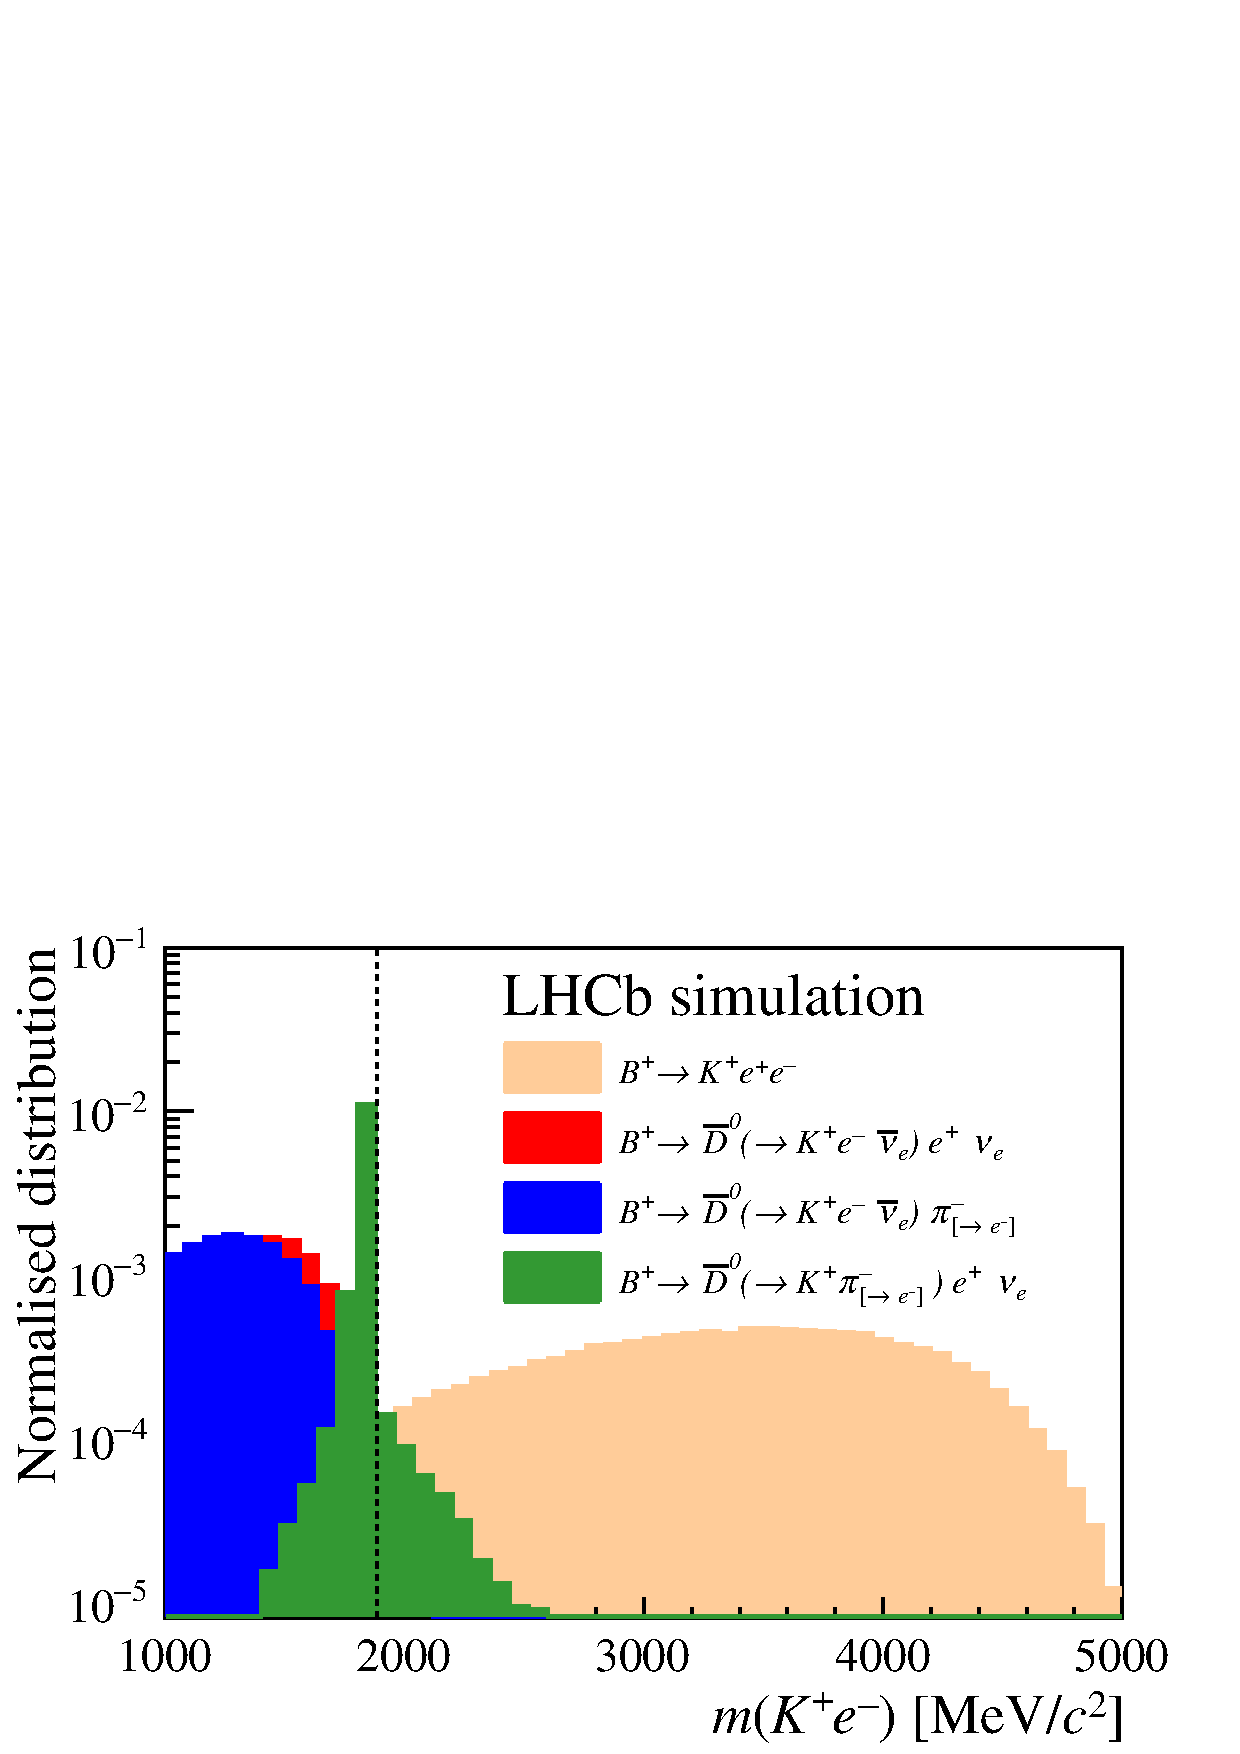
\includegraphics[width=0.48\linewidth]{figures/Fig5a.pdf}
      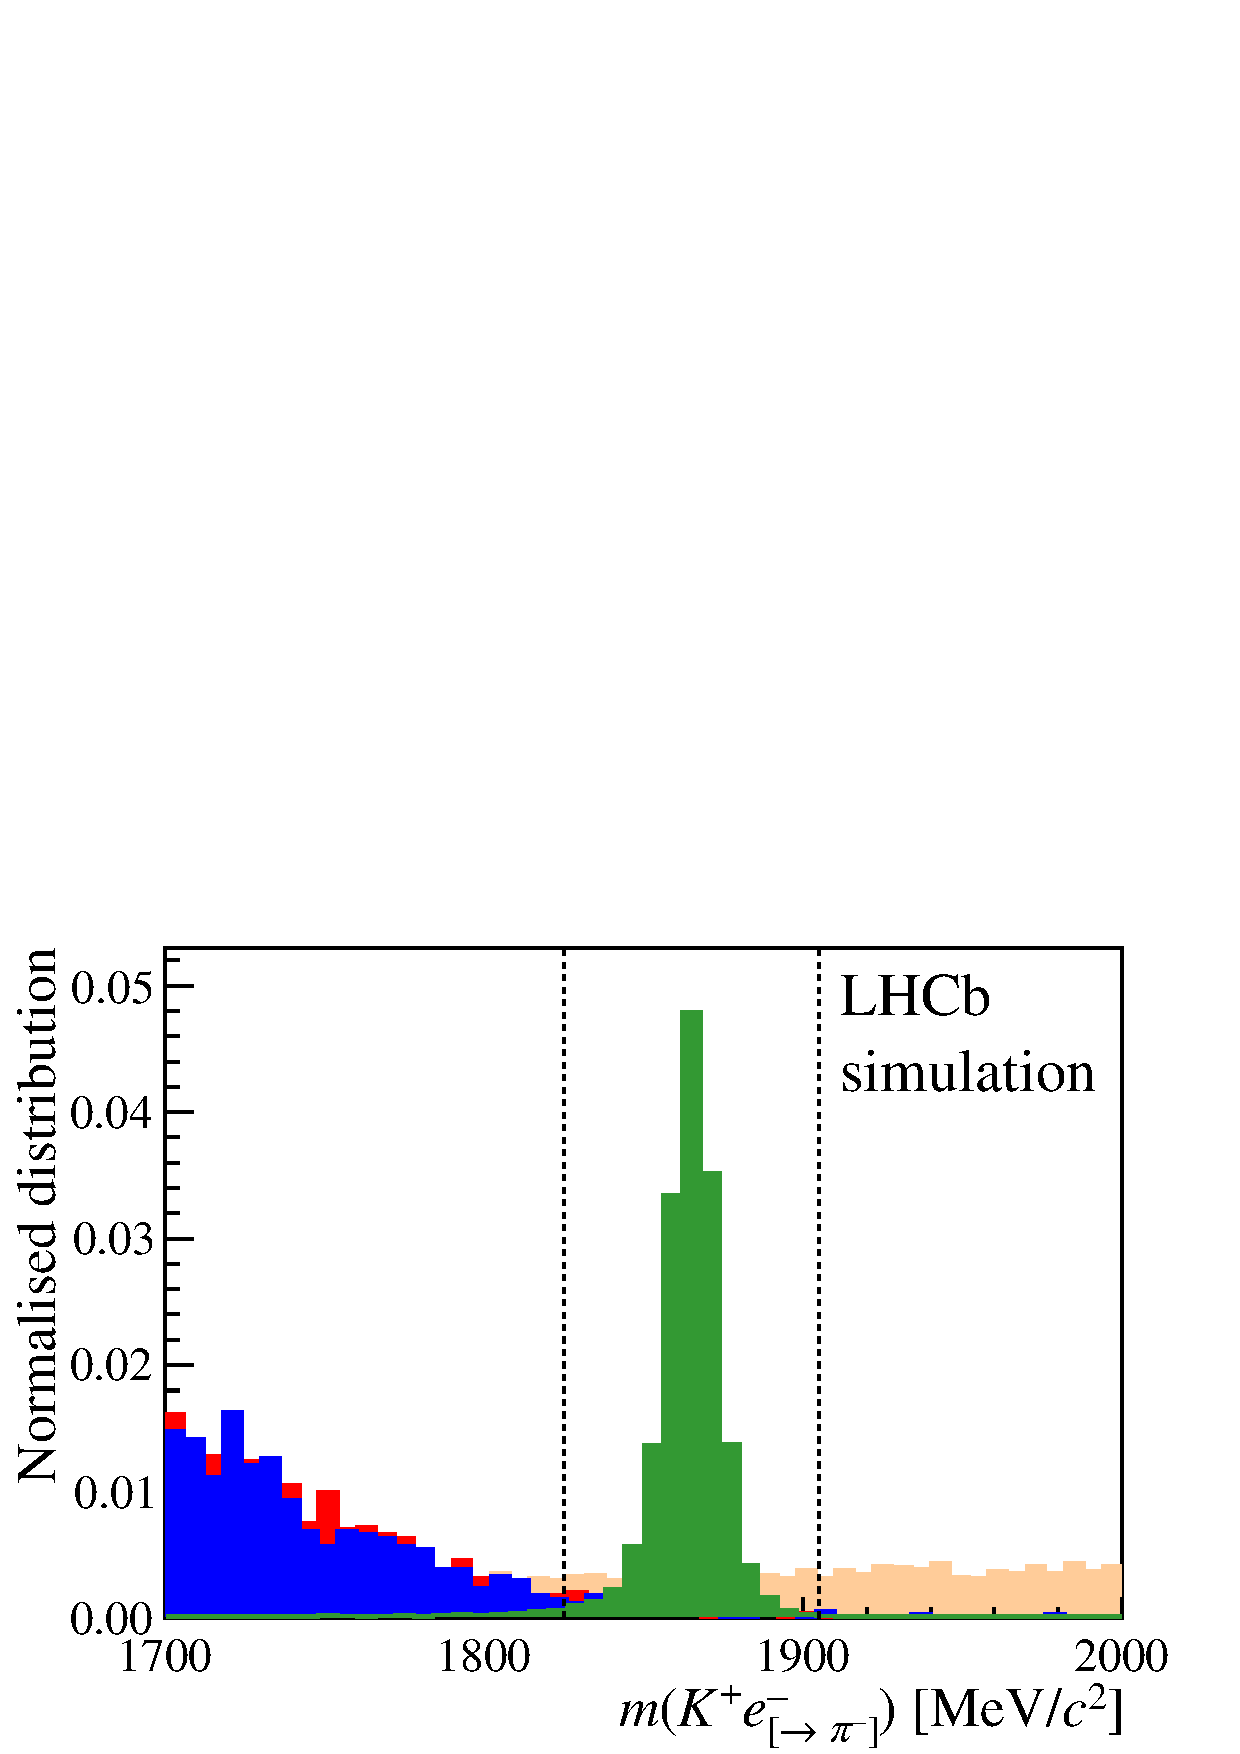
\includegraphics[width=0.48\linewidth]{figures/Fig5b.pdf}
   \end{center}
    \vspace*{-0.5cm}
   \caption{Simulated $K^+e^-$ mass distributions for  signal and various cascade background samples. The distributions are all normalised to unity.  (Left, with log $y$-scale)
   the bremsstrahlung correction to the momentum of the electron is applied, resulting in a tail to the right. The region to the left of the vertical dashed line is rejected. (Right, with linear $y$-scale) the mass is computed only from the track information. The notation $\pi^-_{[\rightarrow e^-]}$ ($e^-_{[\rightarrow \pi^-]}$) is used to denote an electron (pion) that is misidentified as a pion (electron). The region between the dashed vertical lines is rejected. }\label{fig:cascadeVeto}
\end{figure}

Background from other exclusive $B$-hadron decays requires at least two particles to be misidentified. These include the decays \BuKpipi, and misreconstructed \BuJpsiKll and \BuPsiKll decays. In the latter two decays the kaon is misidentified as a lepton and the lepton (of the same electric charge) as a kaon. Such background is reduced to a negligible level by particle-identification criteria. Background from decays with a photon converted into an \epem pair are also negligible due to the \qsq selection.


\subsubsection*{Multivariate selection}

A Boosted Decision Tree (BDT)  algorithm~\cite{Breiman} with gradient boosting~\cite{GradBoost} is used to reduce combinatorial background. For the nonresonant muon mode and for each of the three different trigger categories of the 
nonresonant electron mode, a single BDT classifier is trained for the 7 and $8\tev$ data, and an additional classifier is trained for the $13\tev$ data. The BDT output is not strongly correlated with \qsq and the same classifiers are used to select the respective resonant decays. 
In order to train the classifier, simulated nonresonant \BuKll decays are used as a proxy for the signal and nonresonant \Kll candidates selected from the data with $\mKll > 5.4\gevcc$ are used as a background sample. The $k$-folding technique is used in the training and testing~\cite{Blum:1999:BHB:307400.307439}. 
The classifier includes the following variables:  the  \pt of the \Bp, \Kp and dilepton candidates, and the minimum and maximum \pt of the leptons;  the \Bp, dilepton and \Kp \chisqip with respect to the associated PV, where \chisqip is defined as the difference in the vertex-fit \chisq of the PV reconstructed with and without the considered particle; the minimum and maximum \chisqip of the leptons; the \Bp vertex-fit quality; the statistical significance of the \Bp flight distance; and the angle between the \Bp candidate momentum vector and the direction between the associated PV and the \Bp decay vertex. 
For each of the classifiers, a requirement is placed on the output variable in order to maximise the predicted significance of the nonresonant signal yield. For the electron modes that dictate the \RK precision, this requirement reduces the combinatorial background by approximately $99\%$, while retaining $85\%$ of the signal mode. The muon BDT classifier has similar performance. In both cases the efficiency of the BDT selection has negligible dependence on \mKll in the regions used to determine the event yields. 

\subsubsection*{Calibration of simulation} 

The simulated data used in this analysis are produced using the software described in Refs.~\cite{Sjostrand:2006za,*Sjostrand:2007gs,LHCb-PROC-2010-056,Lange:2001uf,Allison:2006ve, *Agostinelli:2002hh,LHCb-PROC-2011-006}. Bremsstrahlung emission in the decay of particles is simulated using the \photosplusplus software in the default configuration~\cite{ Davidson:2010ew}, which is observed to agree with a full quantum electrodynamics calculation at the level of $1\%$~\cite{Bordone:2016gaq}.

Simulated events are weighted to correct for the imperfect modelling using control channels. The \Bu production kinematics are corrected using \BuJpsiKll events. The particle-identification performance is calibrated using data, where the species of particles in the final state can be unambiguously determined purely on the basis of the kinematics. 
The calibration samples consist of $\decay{\Dstarp}{\Dz(\to\Km\pip)\pip}$, $\decay{\jpsi}{\mumu}$, and \BuJpsiKee decays, from which kaons, muons, and electrons, respectively, can be selected without applying particle-identification requirements. The performance of the particle-identification requirements is then evaluated from the proportion of events in these samples which fulfil the particle-identification selection criteria. The trigger response is corrected using weights applied to simulation as a function of variables relevant to the trigger algorithms. The weights are calculated by requiring that simulated \BuJpsiKll events  exhibit the same trigger performance as the control data. The \BuJpsiKll events selected from the data have also been used to demonstrate control of the electron track-reconstruction efficiency at the percent level~\cite{Aaij:2019vvl}.
Whenever \BuJpsiKll events are used to correct the simulation, the correlations between calibration and measurement samples are taken into account in the results and cross-checks presented in the article. 

\subsubsection*{Likelihood fit} 

An unbinned extended maximum-likelihood fit is made to the \mKee and \mKmm distributions of nonresonant candidates. The value of \RK is a fit parameter, which is related to the signal yields and efficiencies according to,  
\begin{eqnarray}
    \label{eq:RKdetail}
       \RK &=&\frac{N(\BuKmm)}{\varepsilon(\BuKmm)}\cdot\frac{\varepsilon(\BuKee)}{N(\BuKee)} \times \nonumber\\
 & & \frac{\varepsilon(\BuJpsiKmm)}{N(\BuJpsiKmm)}\cdot\frac{N(\BuJpsiKee)}{\varepsilon(\BuJpsiKee)} \,, 
\end{eqnarray}
\noindent where $N(X)$  indicates the  yield  of  decay  mode $X$,  which  is  obtained from a fit to the invariant mass \mKll (or \mKllconst) with a suitable requirement on \qsq, and $\varepsilon(X)$ is the efficiency for selecting decay mode $X$. In order to take into account the correlation between the selection efficiencies, the \mKee and \mKmm distributions of nonresonant candidates in each of the different trigger categories and data-taking periods are fitted simultaneously. 

The mass-shape parameters are derived from the calibrated simulation. The four signal modes are modelled by multiple Gaussian functions with  power-law tails on both sides of the peak~\cite{Skwarnicki:1986xj,Santos:2013gra} although the differing detector response gives different shapes for the electron and muon modes. The signal mass shapes of the electron modes are described with the sum of three distributions, which model whether the ECAL energy deposit from a bremsstrahlung photon was added to both, either, or neither of the \epm candidates. The expected values from simulated events are used to constrain the fraction of signal decays in each of these categories.

Data are used to correct the simulated $K\pi$ mass spectrum for \BuBdKpiplusee and \BuBdKpijpsi decays~\cite{LHCb-PAPER-2016-025}. The calibrated simulation is used subsequently to obtain the \mKll mass shape and relative fractions of these background components. In order to accommodate possible lepton-universality violation in these partially reconstructed processes, which are underpinned by the same $\bquarkbar\to\squarkbar$ quark-level transitions as those of interest, the overall yield of such decays is left to vary freely in the fit. The shape of the \BuJpsipi background contribution is taken from simulation but the size with respect to the \BuJpsiK mode is constrained using the known ratio of the relevant branching fractions~\cite{LHCb-PAPER-2016-051, PDG2020} and efficiencies.

In the fits to nonresonant \BuKee candidates, the mass shape of the background from \BuJpsiKee decays with an emitted photon that is not reconstructed is also taken from simulation and, adjusting for the relevant selection efficiency, its yield is constrained to the value from the fit to the resonant mode within its uncertainty.   
In all fits, the combinatorial background is modelled with an exponential function with a freely varying yield and shape.

The fits to the nonresonant (resonant) decay modes in different data-taking periods and trigger categories are shown in Fig.~\ref{fig:nonresfits_categories}  (Fig.~\ref{fig:resfits_categories}).
For the resonant modes the results from independent fits to each period/category are shown. Conversely, the nonresonant distributions show the projections from the simultaneous fit across data taking periods and trigger categories that is used to obtain \RK. The fitted yields for the resonant and nonresonant decays are given in Table~\ref{tab:yields}. 

\begin{table}[b]
\centering
\caption{Yields of the  nonresonant and resonant decay modes obtained from the fits to the data.} \label{tab:yields}
\begin{tabular}{lc}
\toprule
Decay mode  &   Yield             \\
\midrule
\BuKee      &   $\phantom{0\,00}1\,640 \pm \phantom{0\,0}70$ \\
\BuKmm      &   $\phantom{0\,00}3\,850 \pm \phantom{0\,0}70$ \\
\BuJpsiKee  &   $\phantom{0\,}743\,300 \pm \phantom{0\,}900$ \\
\BuJpsiKmm  &   $2\,288\,500 \pm 1\,500$      \\
\bottomrule
\end{tabular}
\end{table}


\begin{figure}
    \centering
    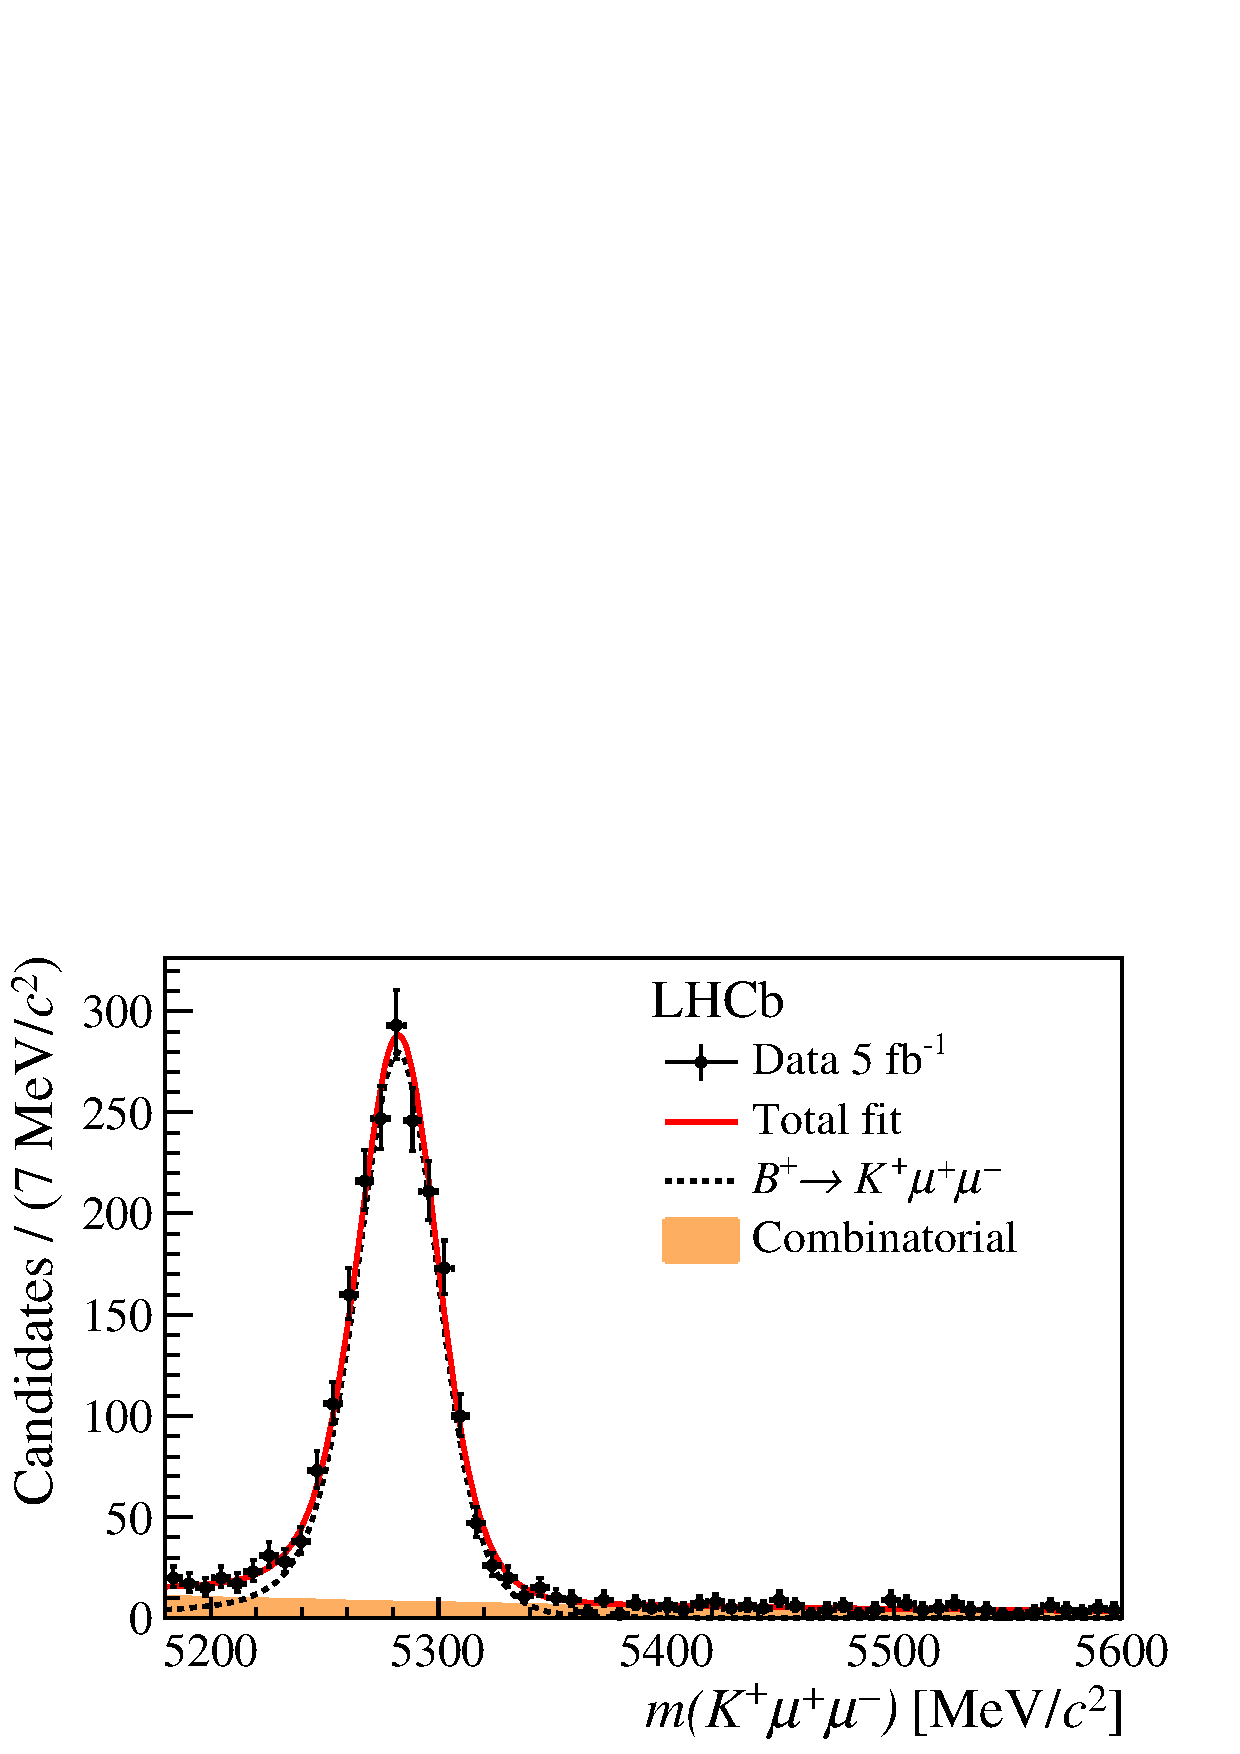
\includegraphics[width=0.45\textwidth]{figures/Fig6a.pdf}
    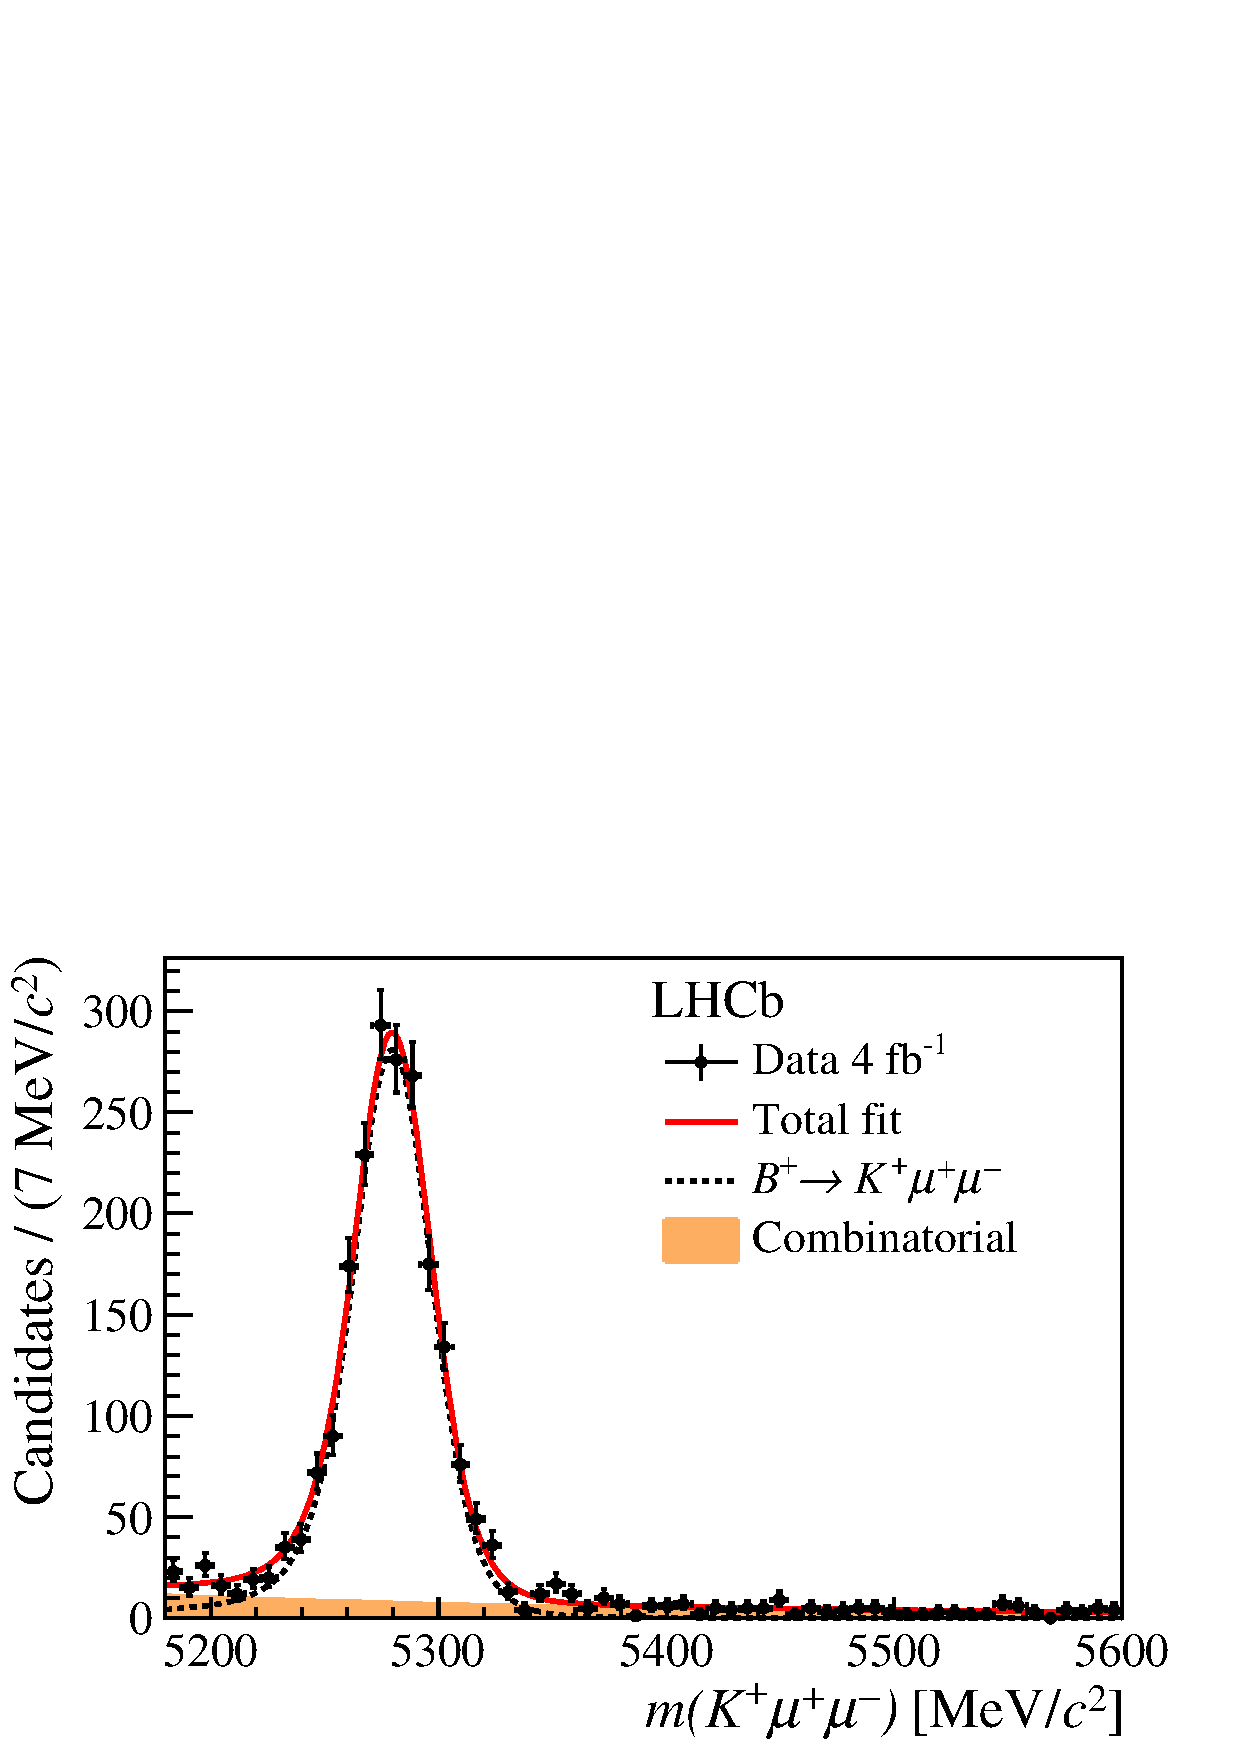
\includegraphics[width=0.45\textwidth]{figures/Fig6b.pdf}

    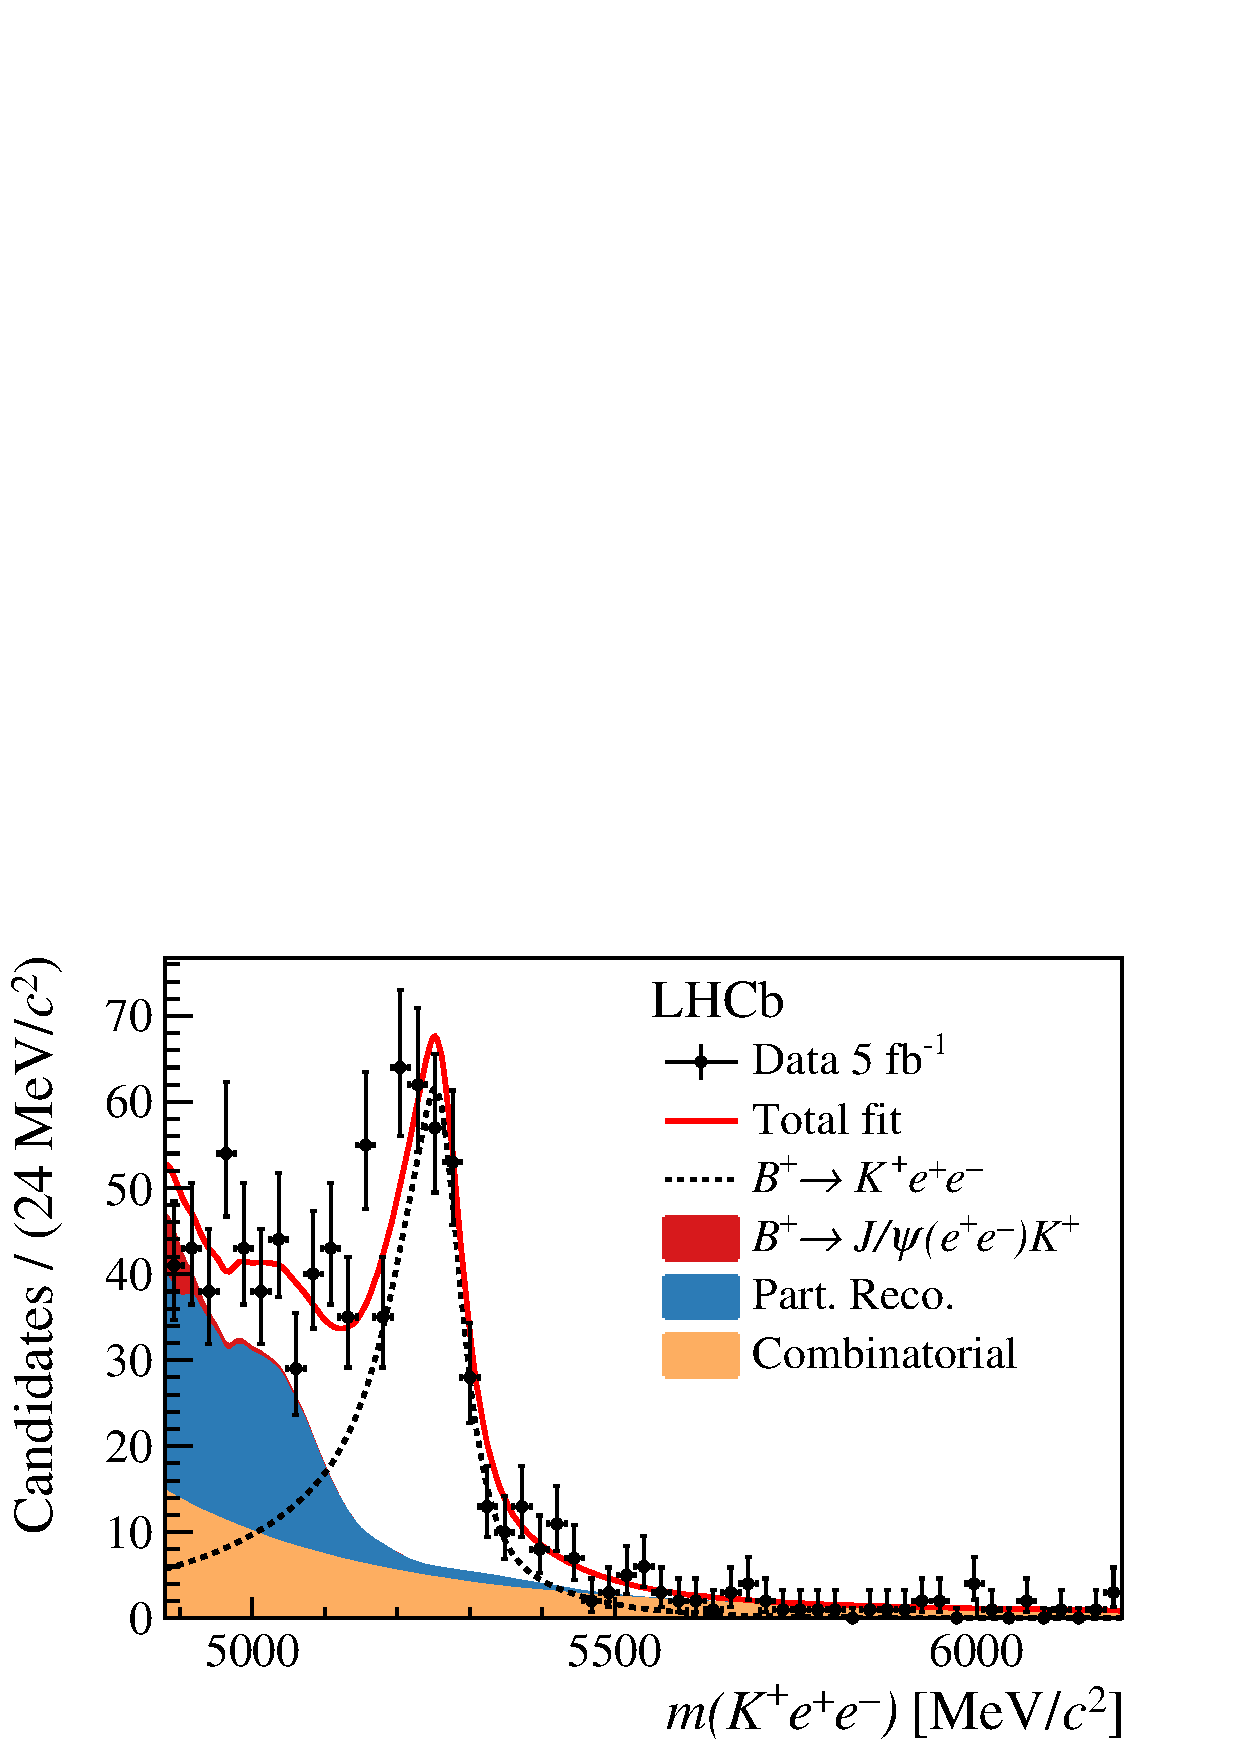
\includegraphics[width=0.45\textwidth]{figures/Fig6c.pdf}
    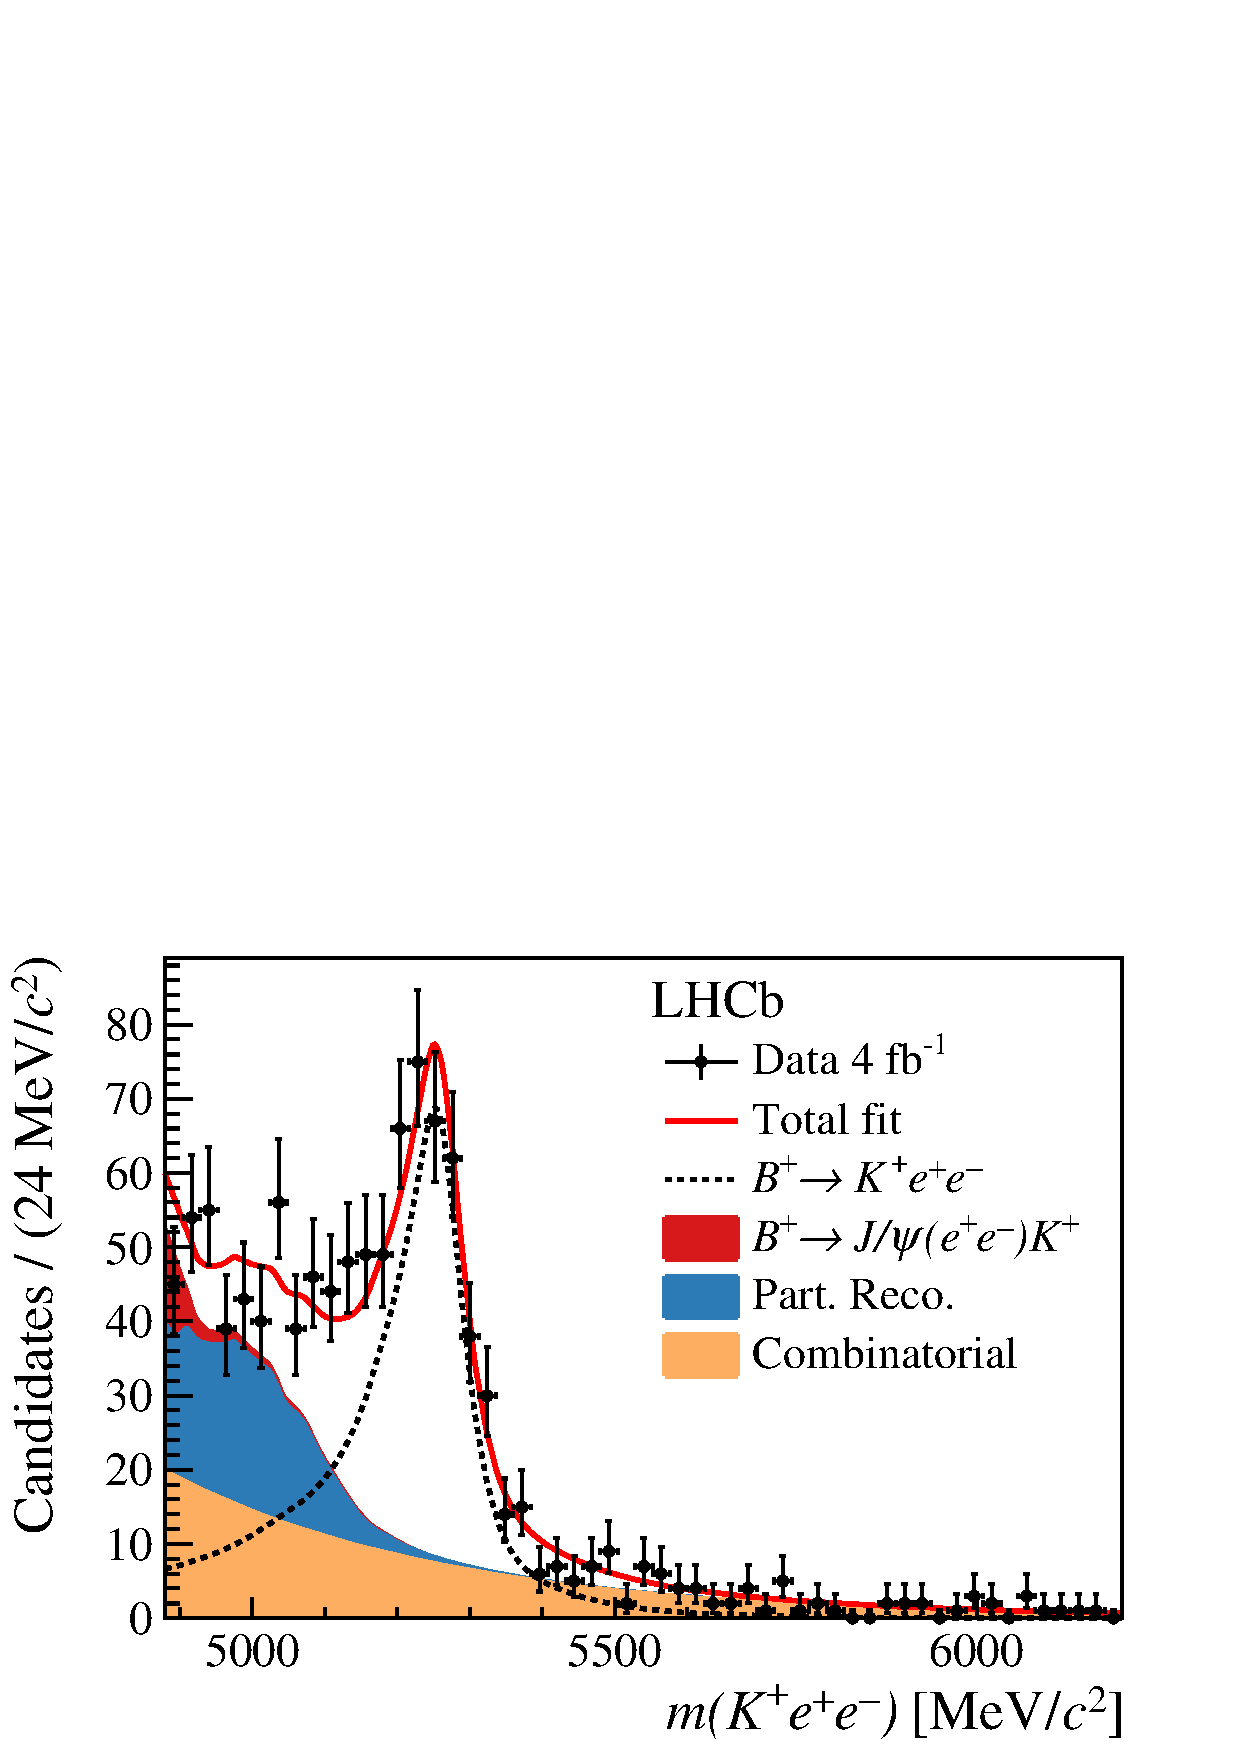
\includegraphics[width=0.45\textwidth]{figures/Fig6d.pdf}
    
    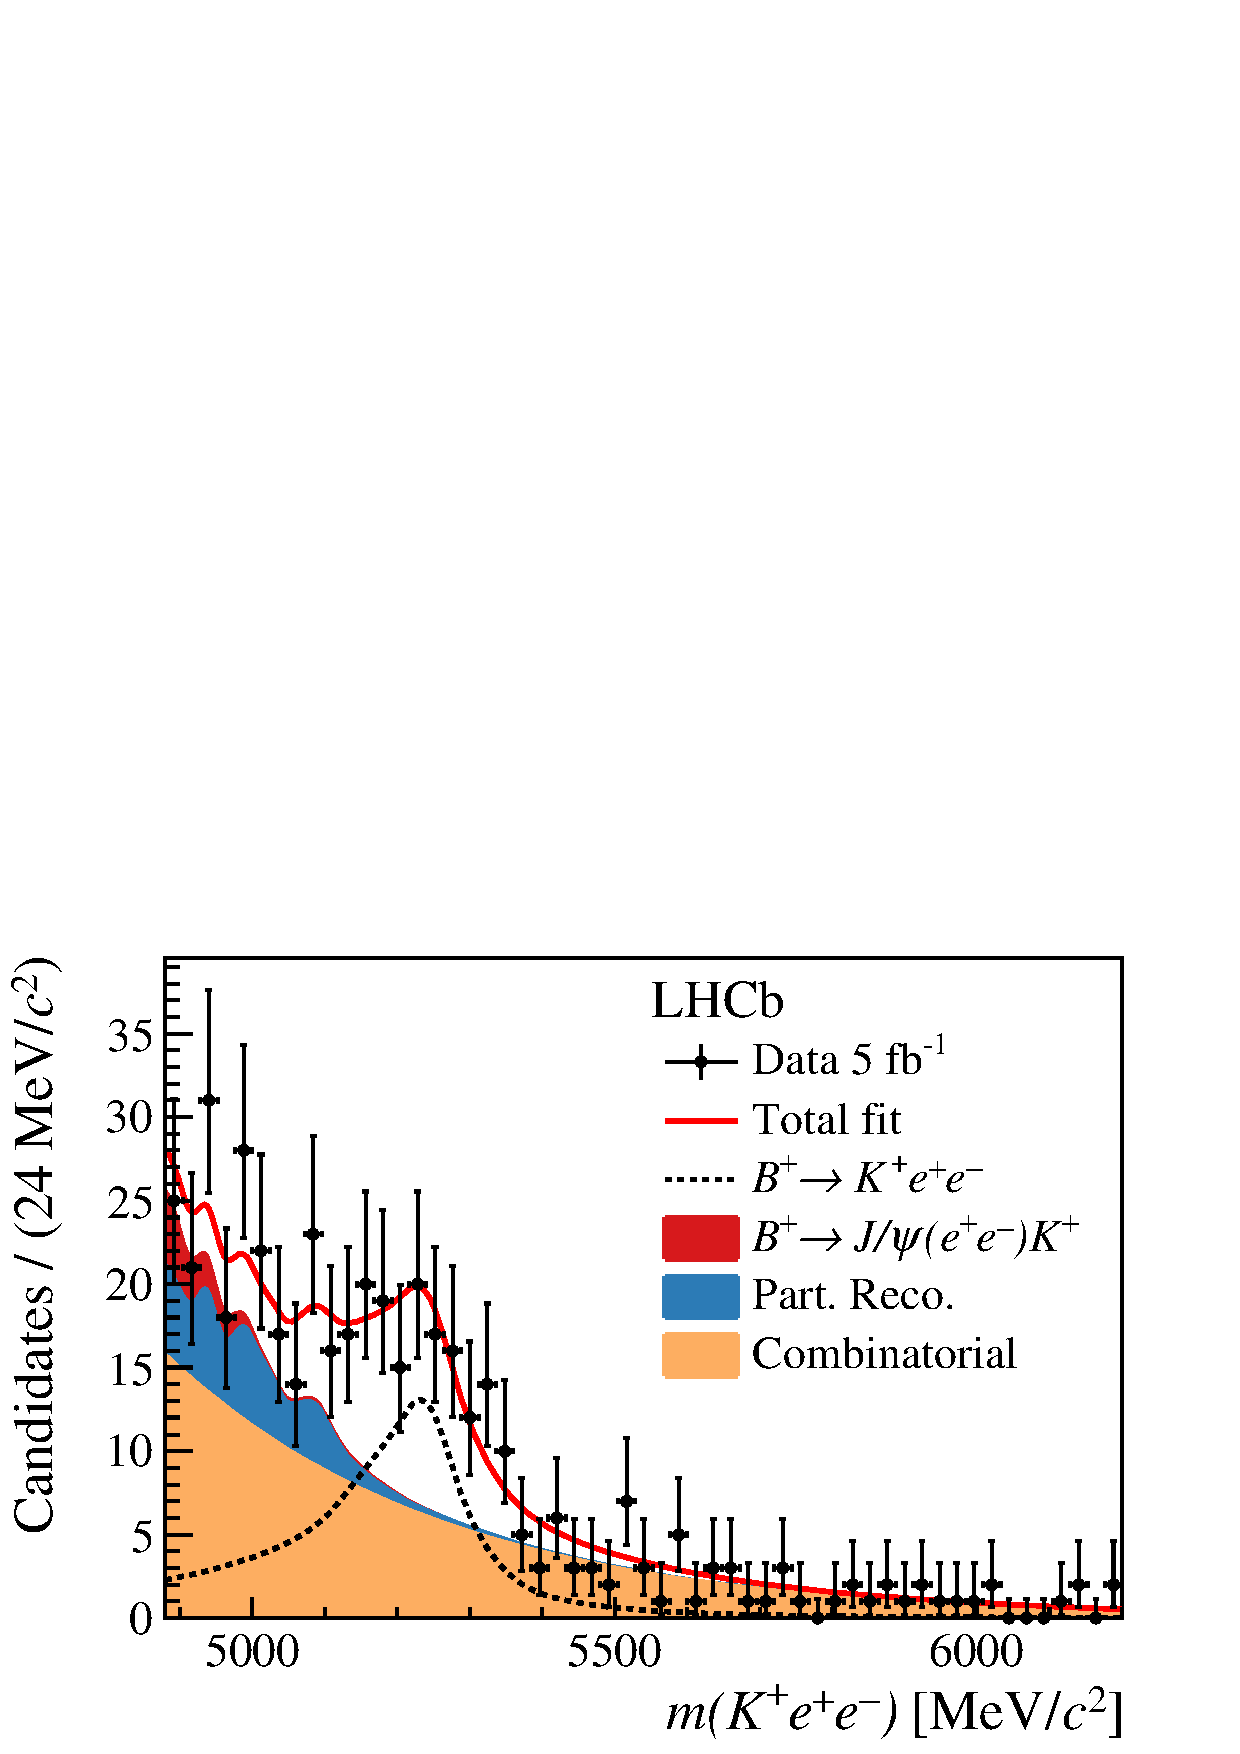
\includegraphics[width=0.45\textwidth]{figures/Fig6e.pdf}
    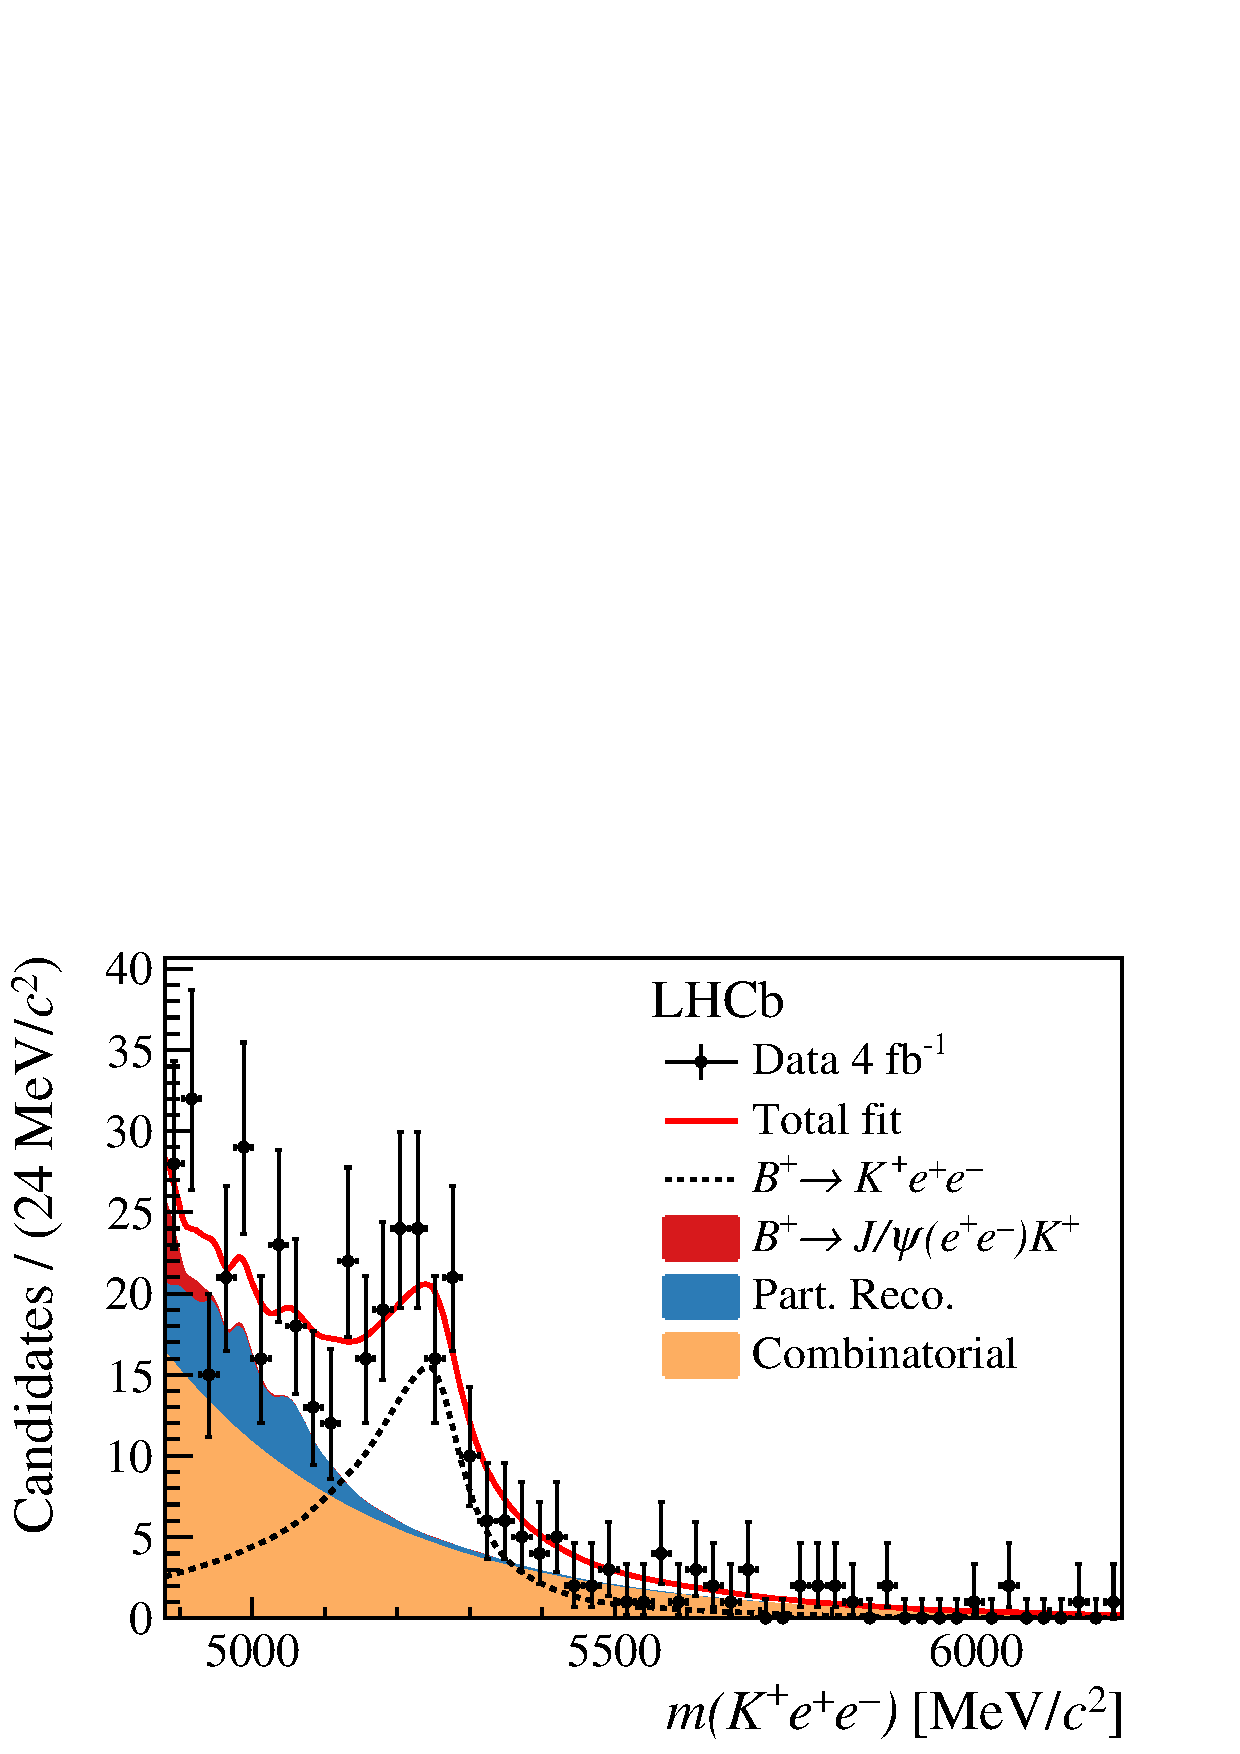
\includegraphics[width=0.45\textwidth]{figures/Fig6f.pdf}
    
    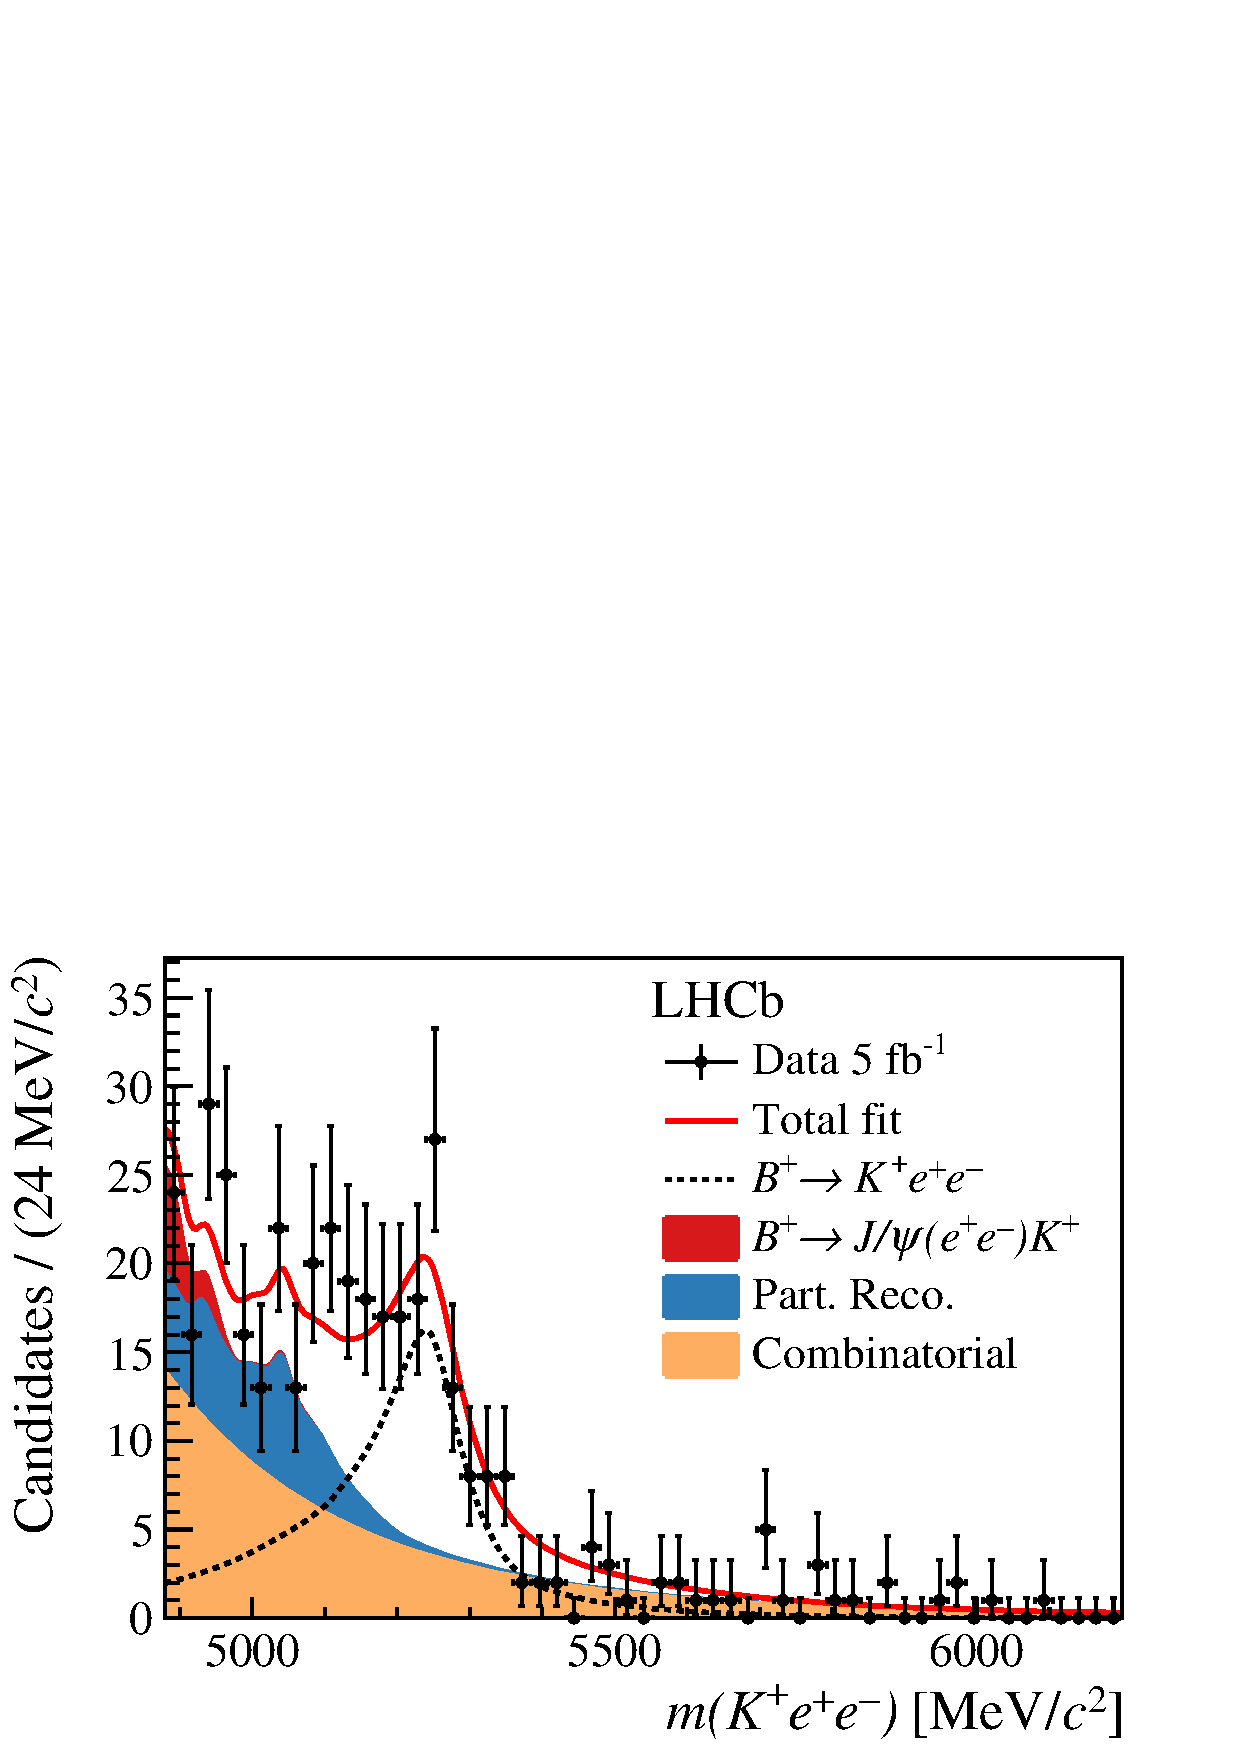
\includegraphics[width=0.45\textwidth]{figures/Fig6g.pdf}
    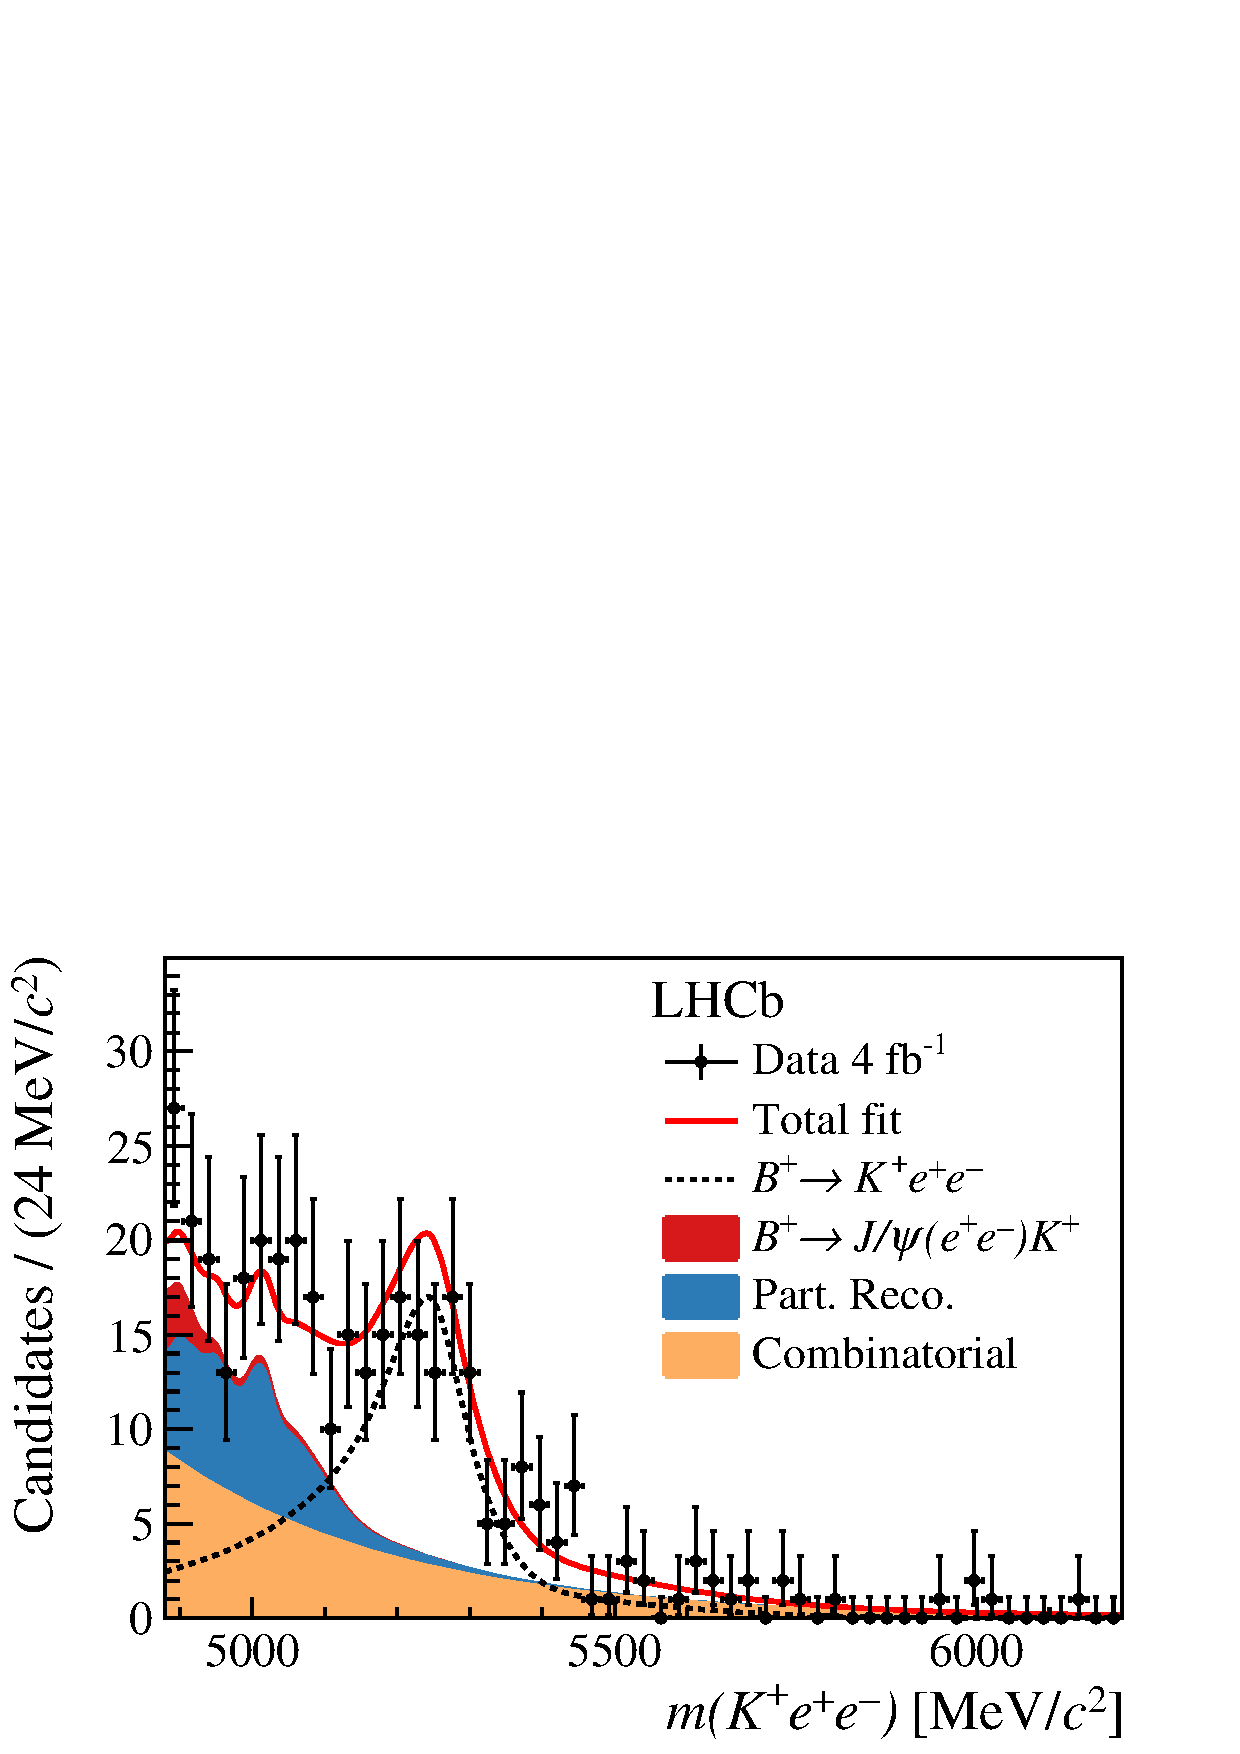
\includegraphics[width=0.45\textwidth]{figures/Fig6h.pdf}
    \caption{Candidate invariant mass distributions. Distribution of the invariant mass \mKll for nonresonant candidates in the (left) sample previously analysed~\cite{LHCb-PAPER-2019-009} and (right) the new data sample. The top row shows the fit to the muon modes and the subsequent rows the fits to the electron modes triggered by (second row) one of the electrons, (third row) the kaon and (last row) by other particles in the event. The fit projections are superimposed.
    }
    \label{fig:nonresfits_categories}
\end{figure}


\begin{figure}
    \centering
    % \includegraphics[width=0.45\textwidth]{figures/FigS5a.pdf}
    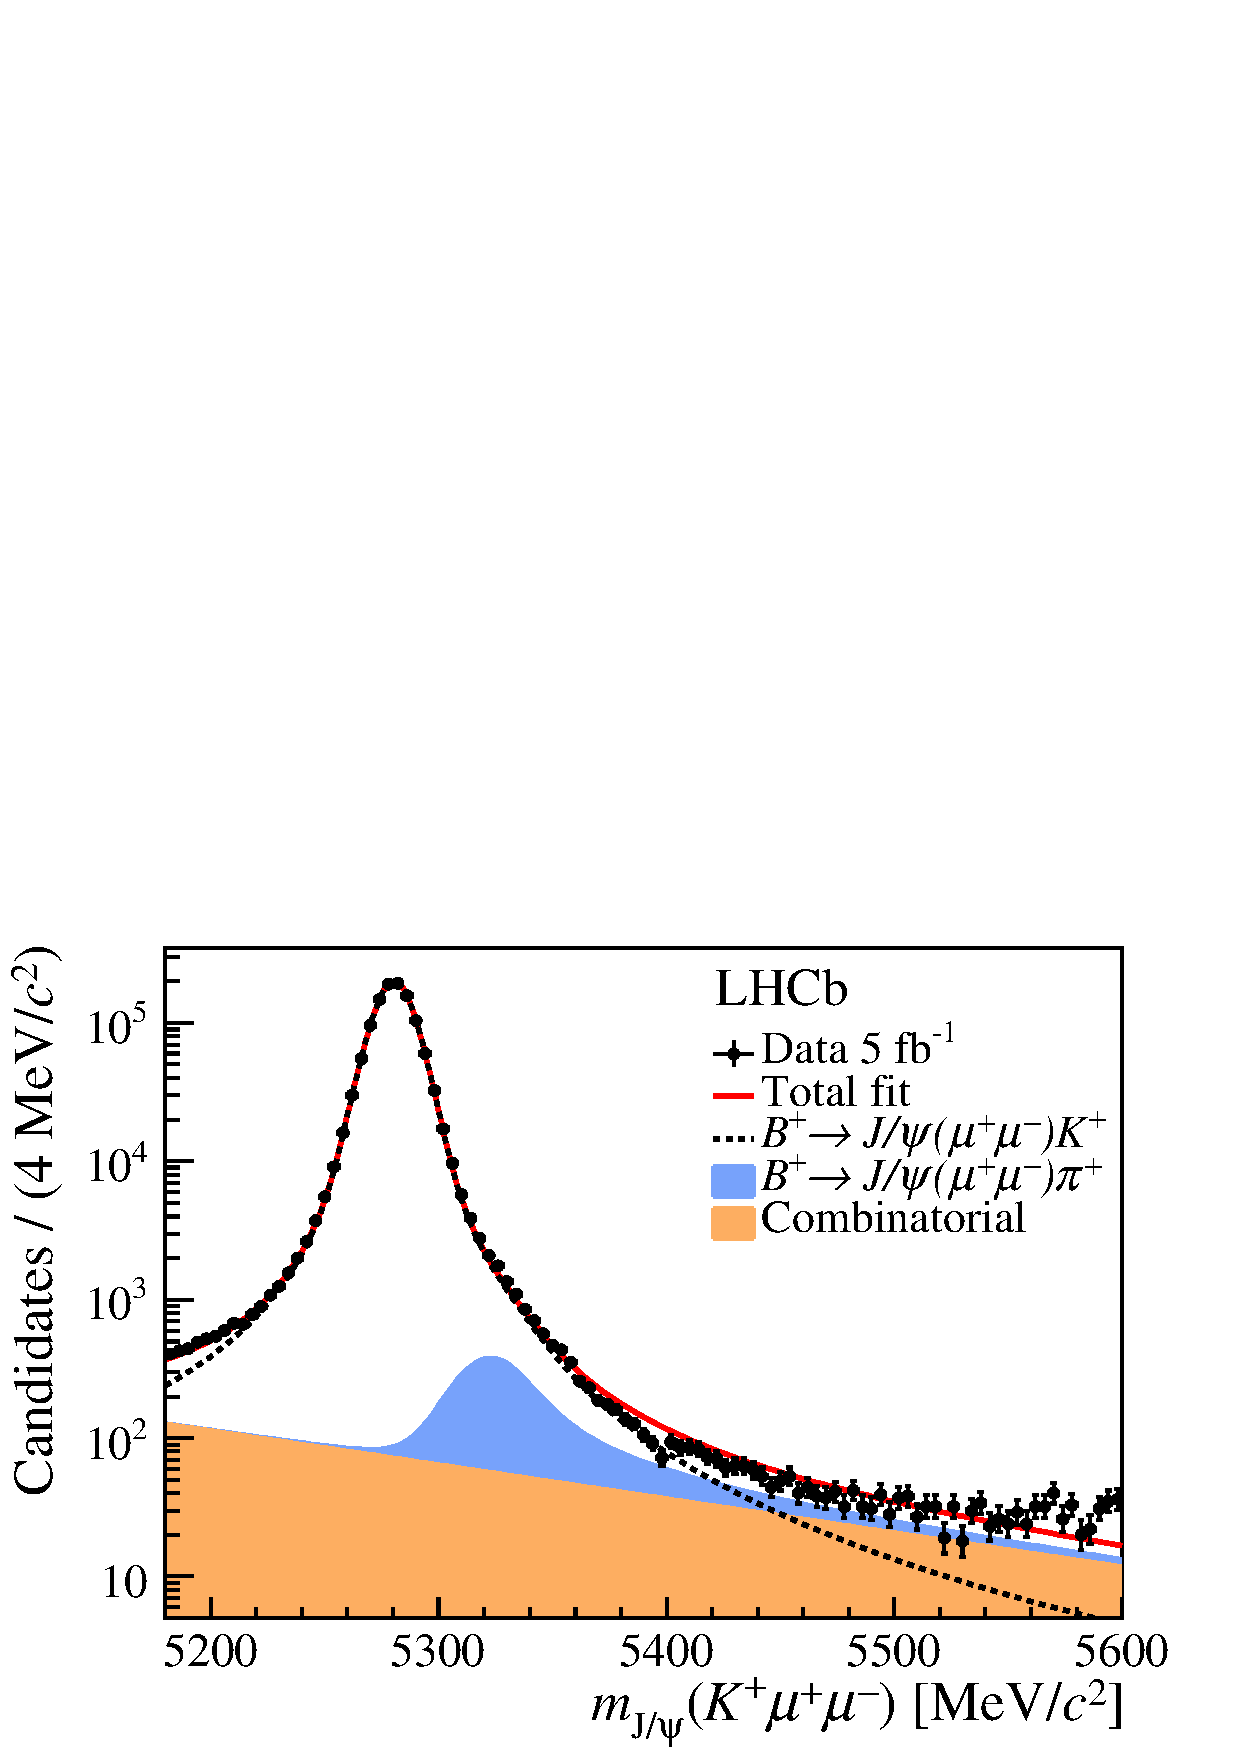
\includegraphics[width=0.45\textwidth]{figures/Fig7a.pdf}
    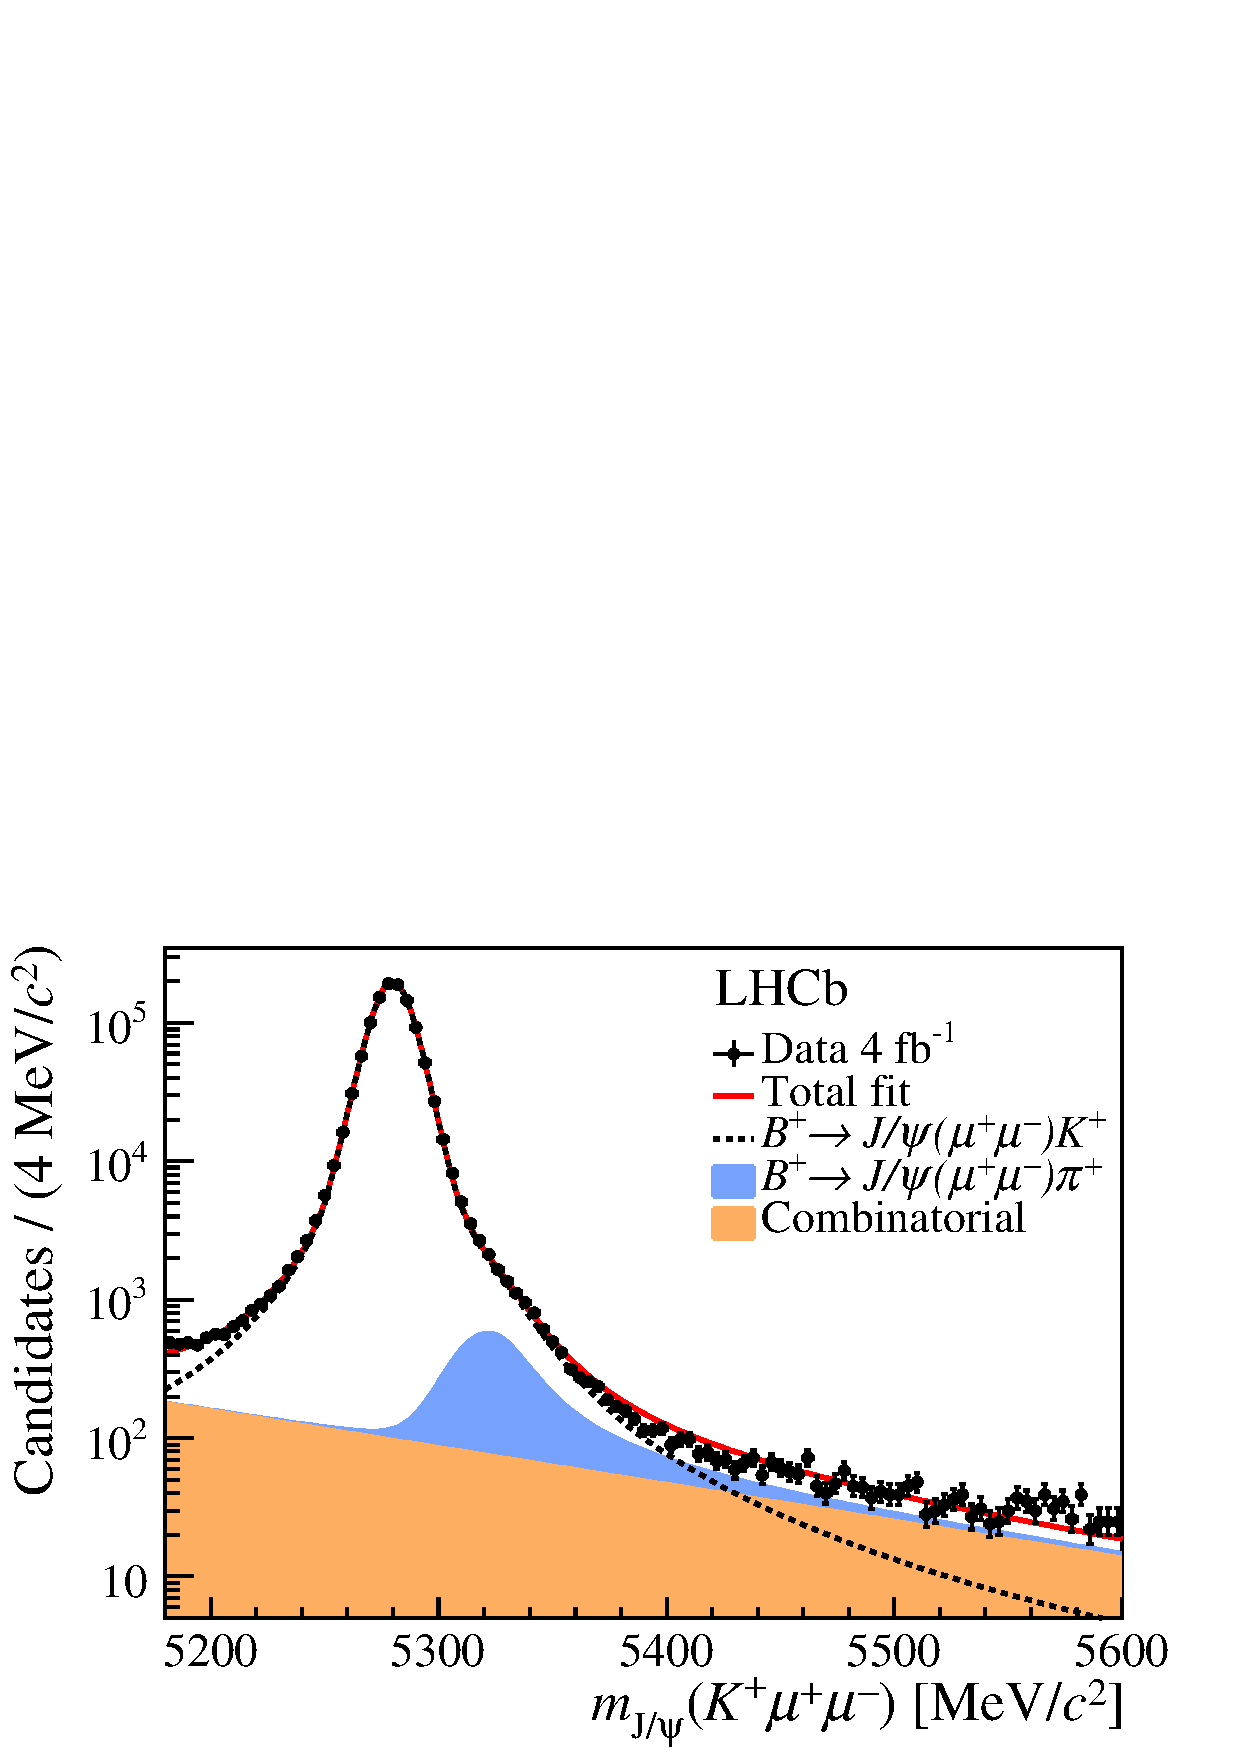
\includegraphics[width=0.45\textwidth]{figures/Fig7b.pdf}
    
    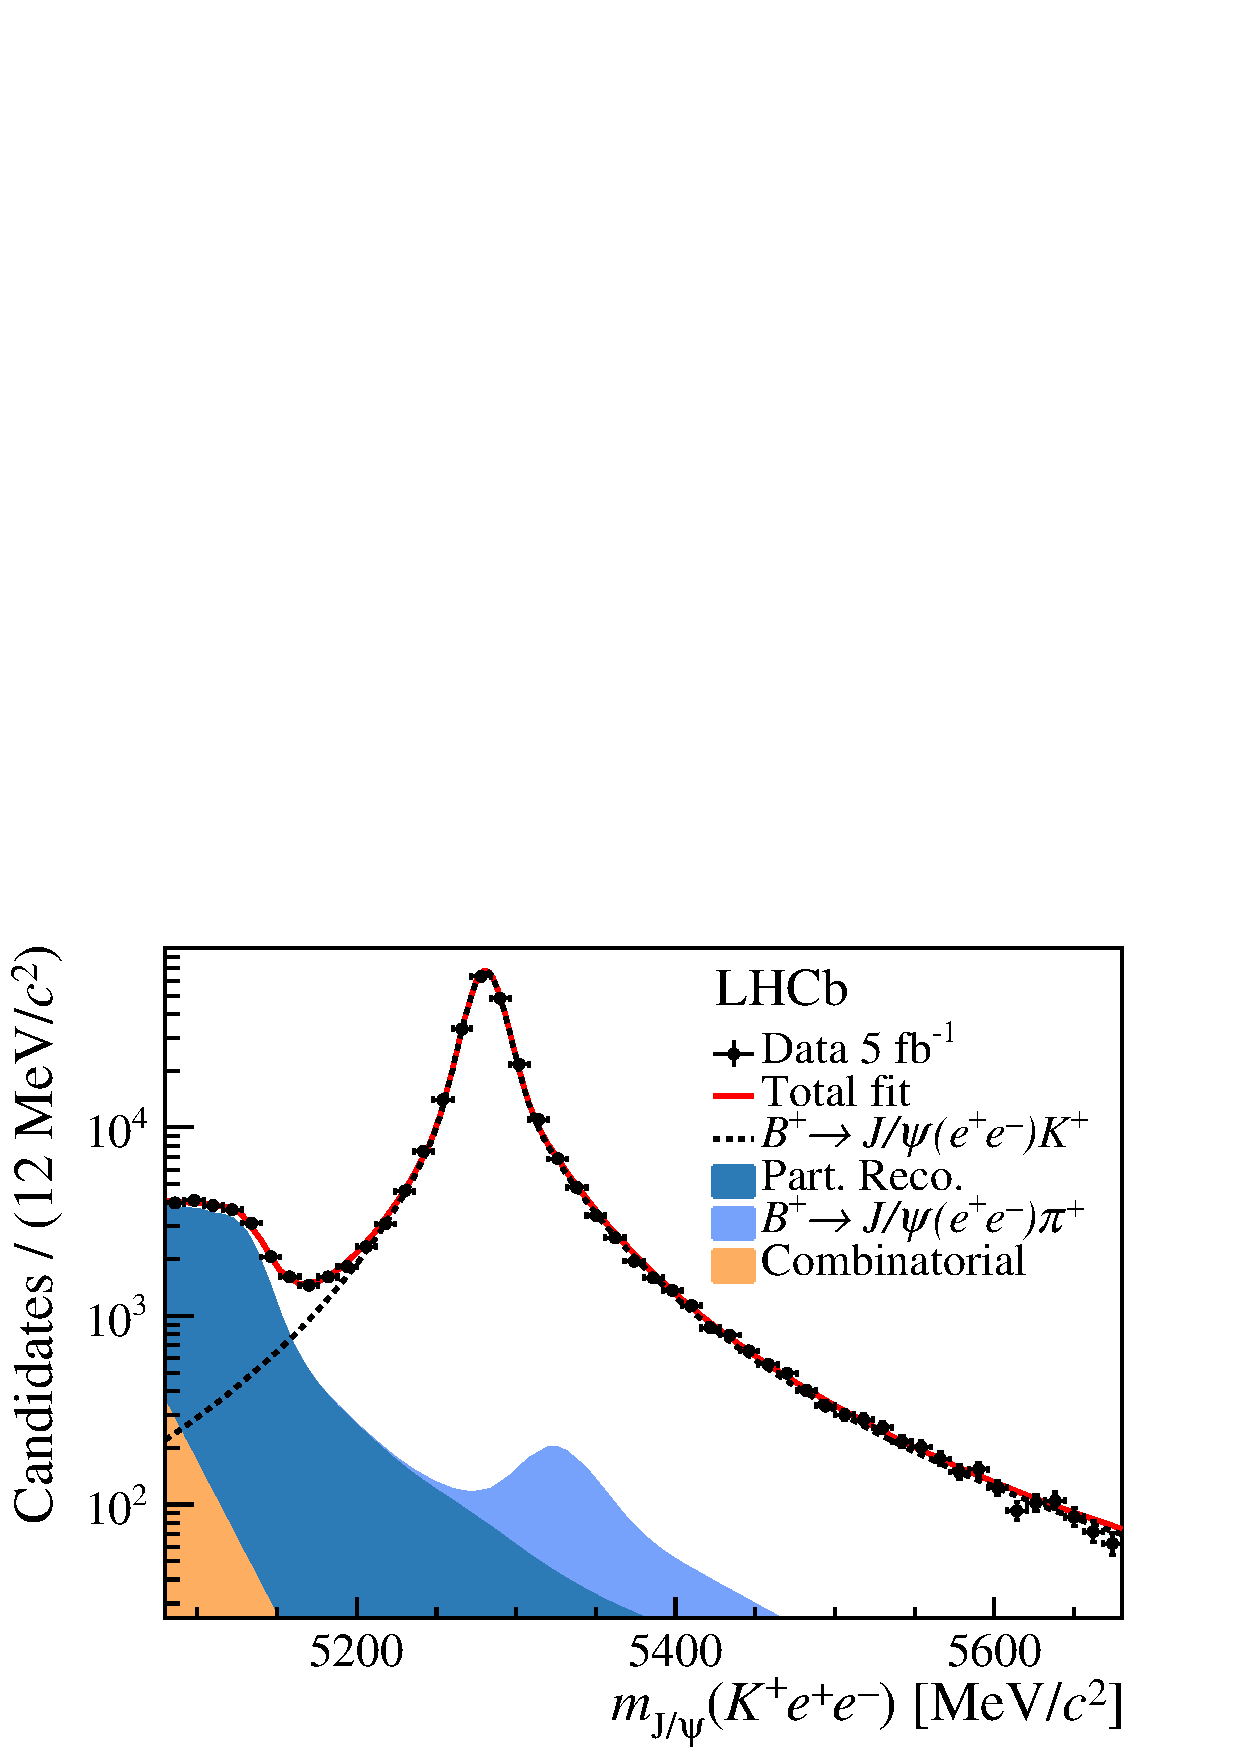
\includegraphics[width=0.45\textwidth]{figures/Fig7c.pdf}
    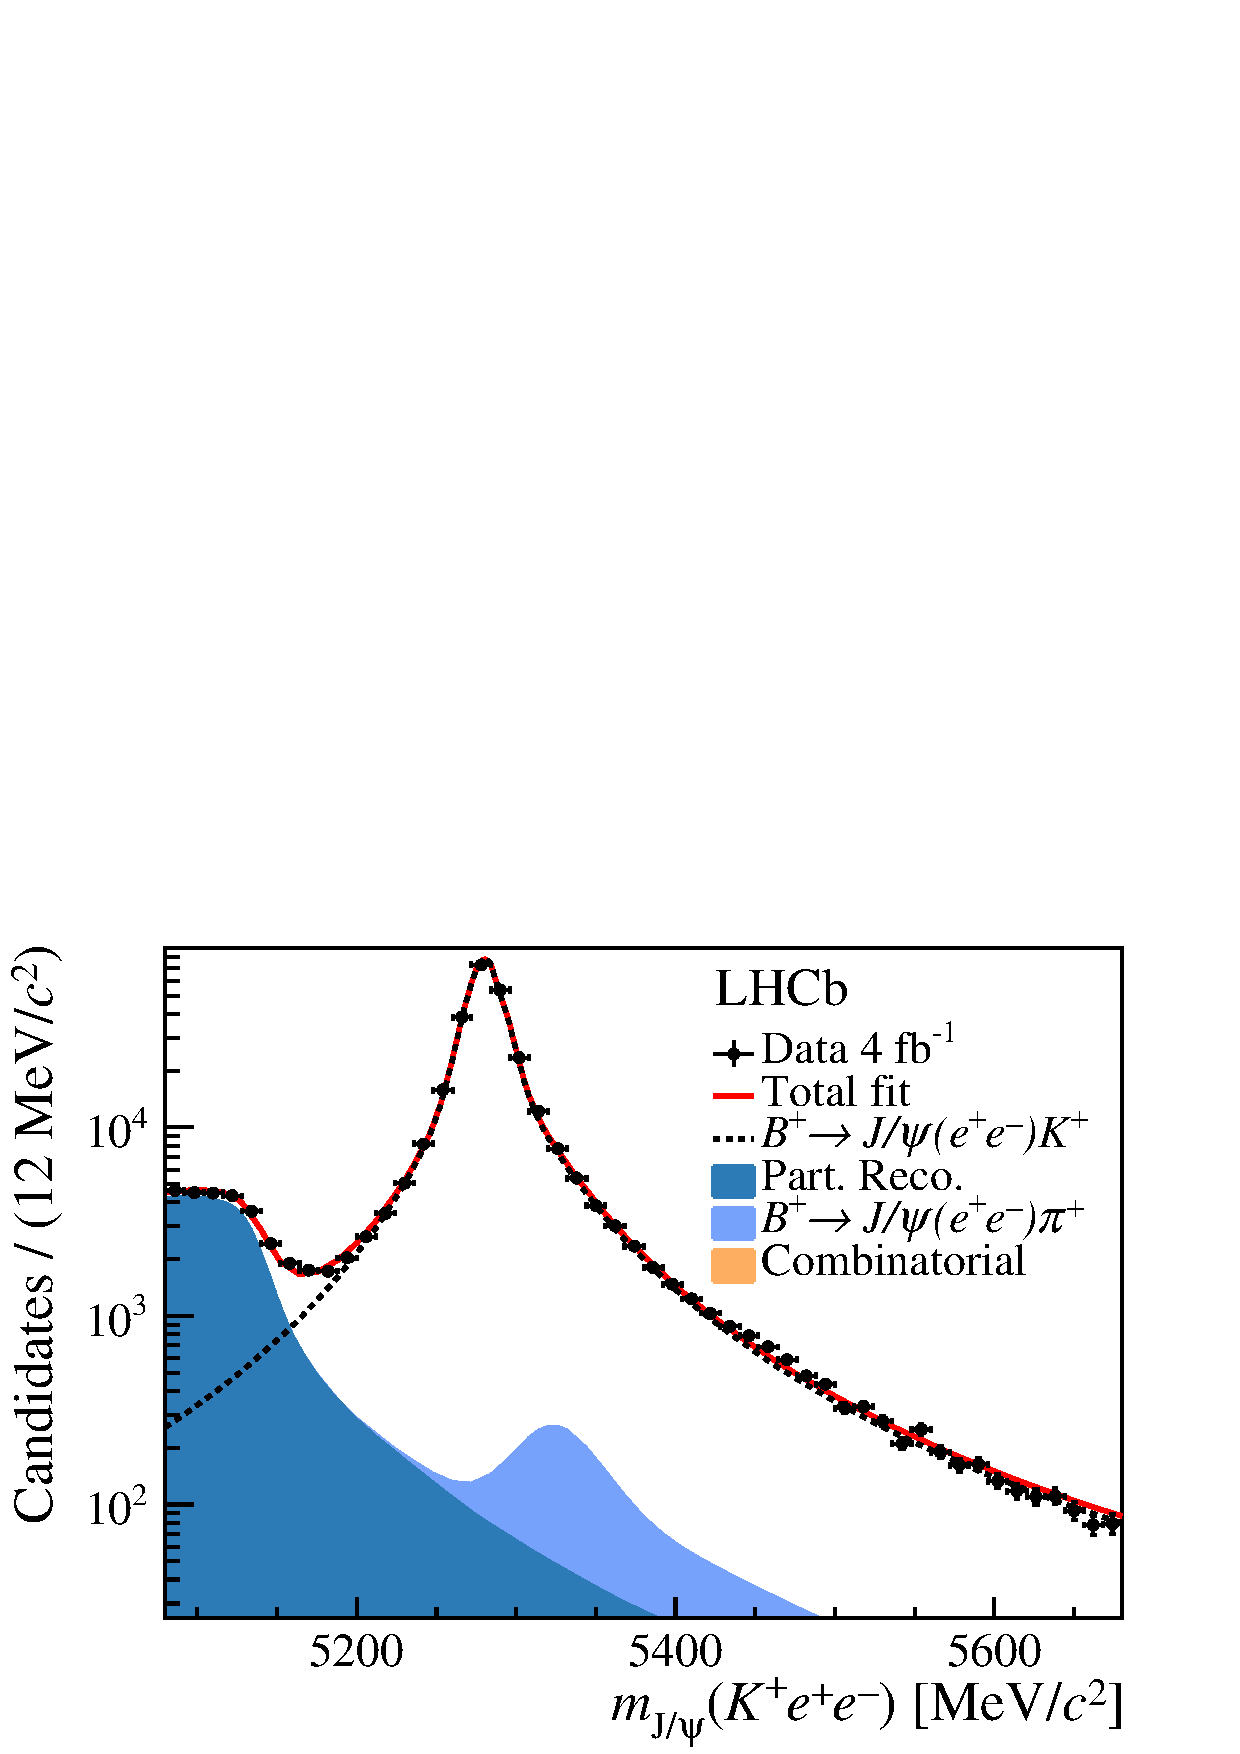
\includegraphics[width=0.45\textwidth]{figures/Fig7d.pdf}
    
    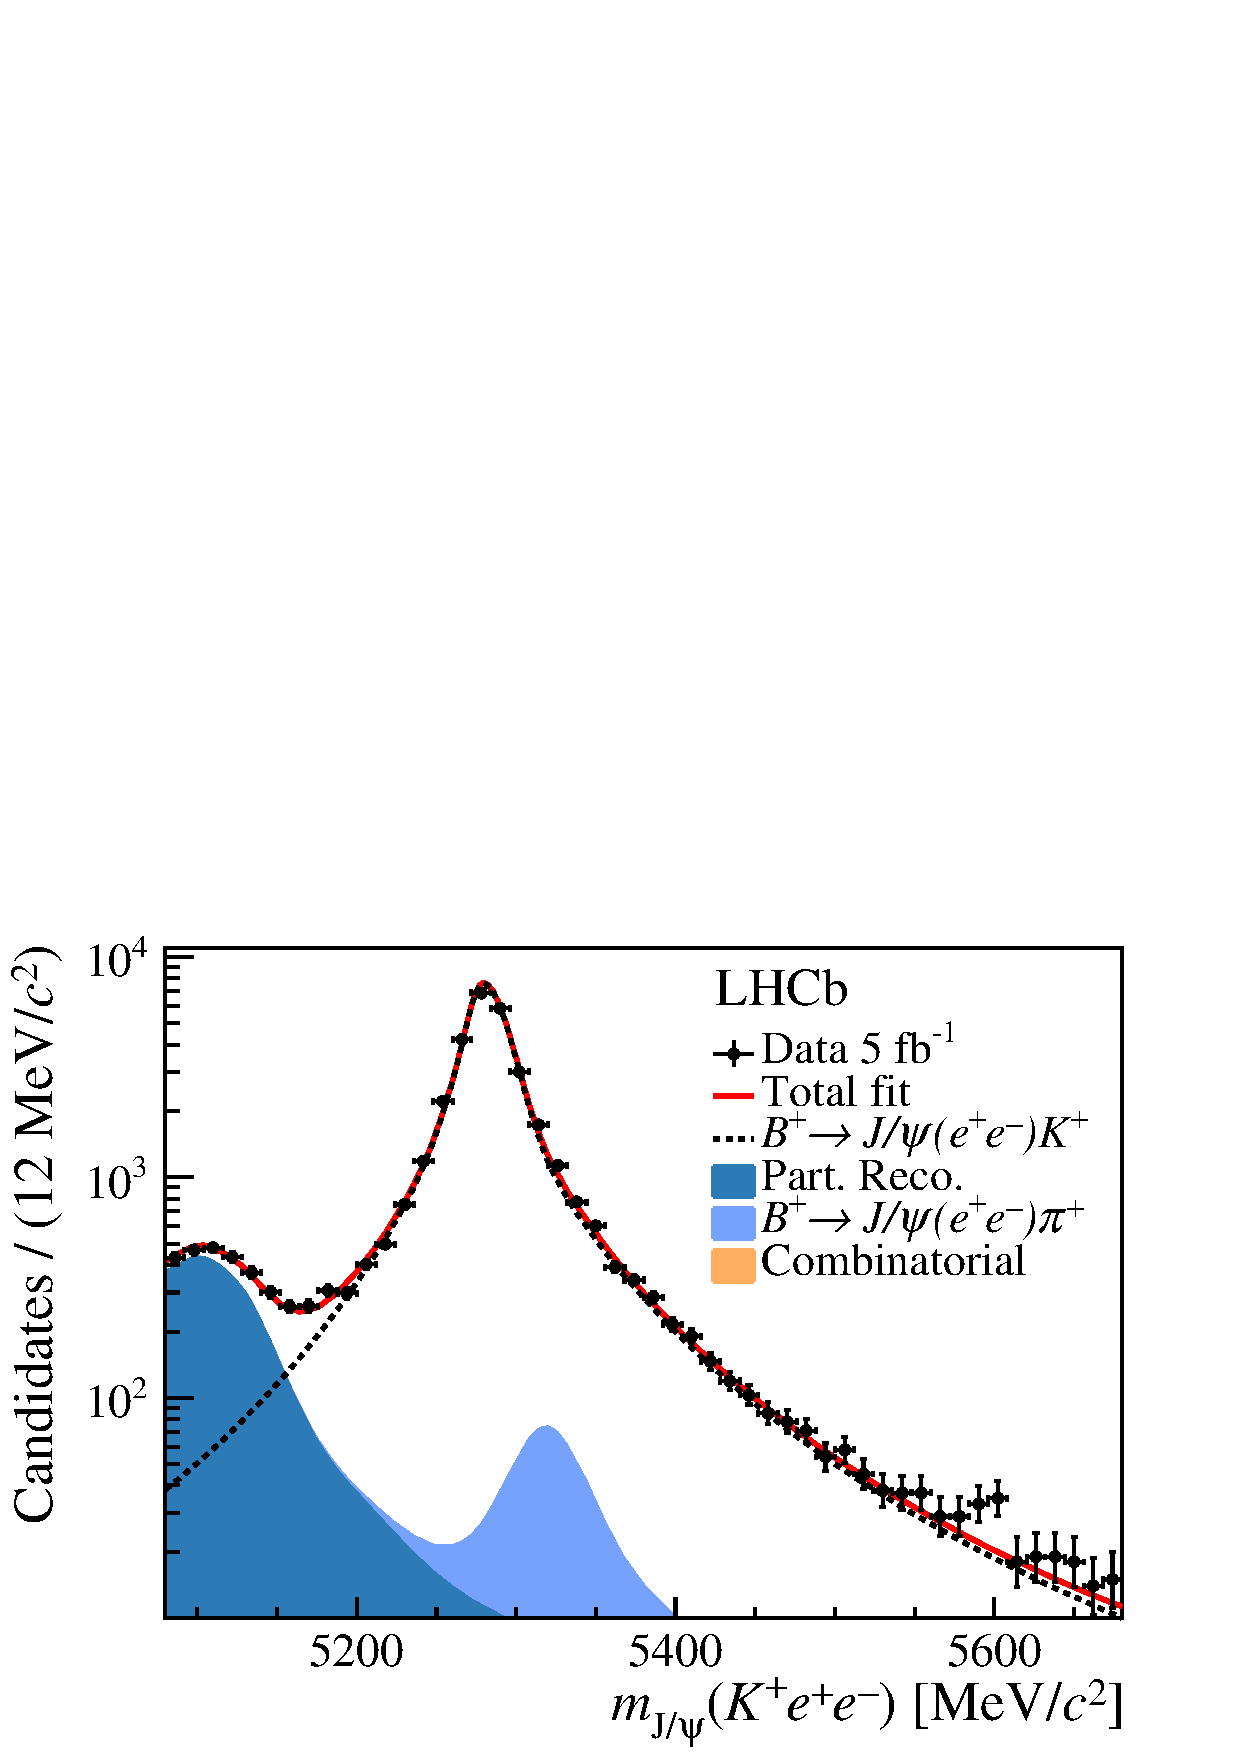
\includegraphics[width=0.45\textwidth]{figures/Fig7e.pdf}
    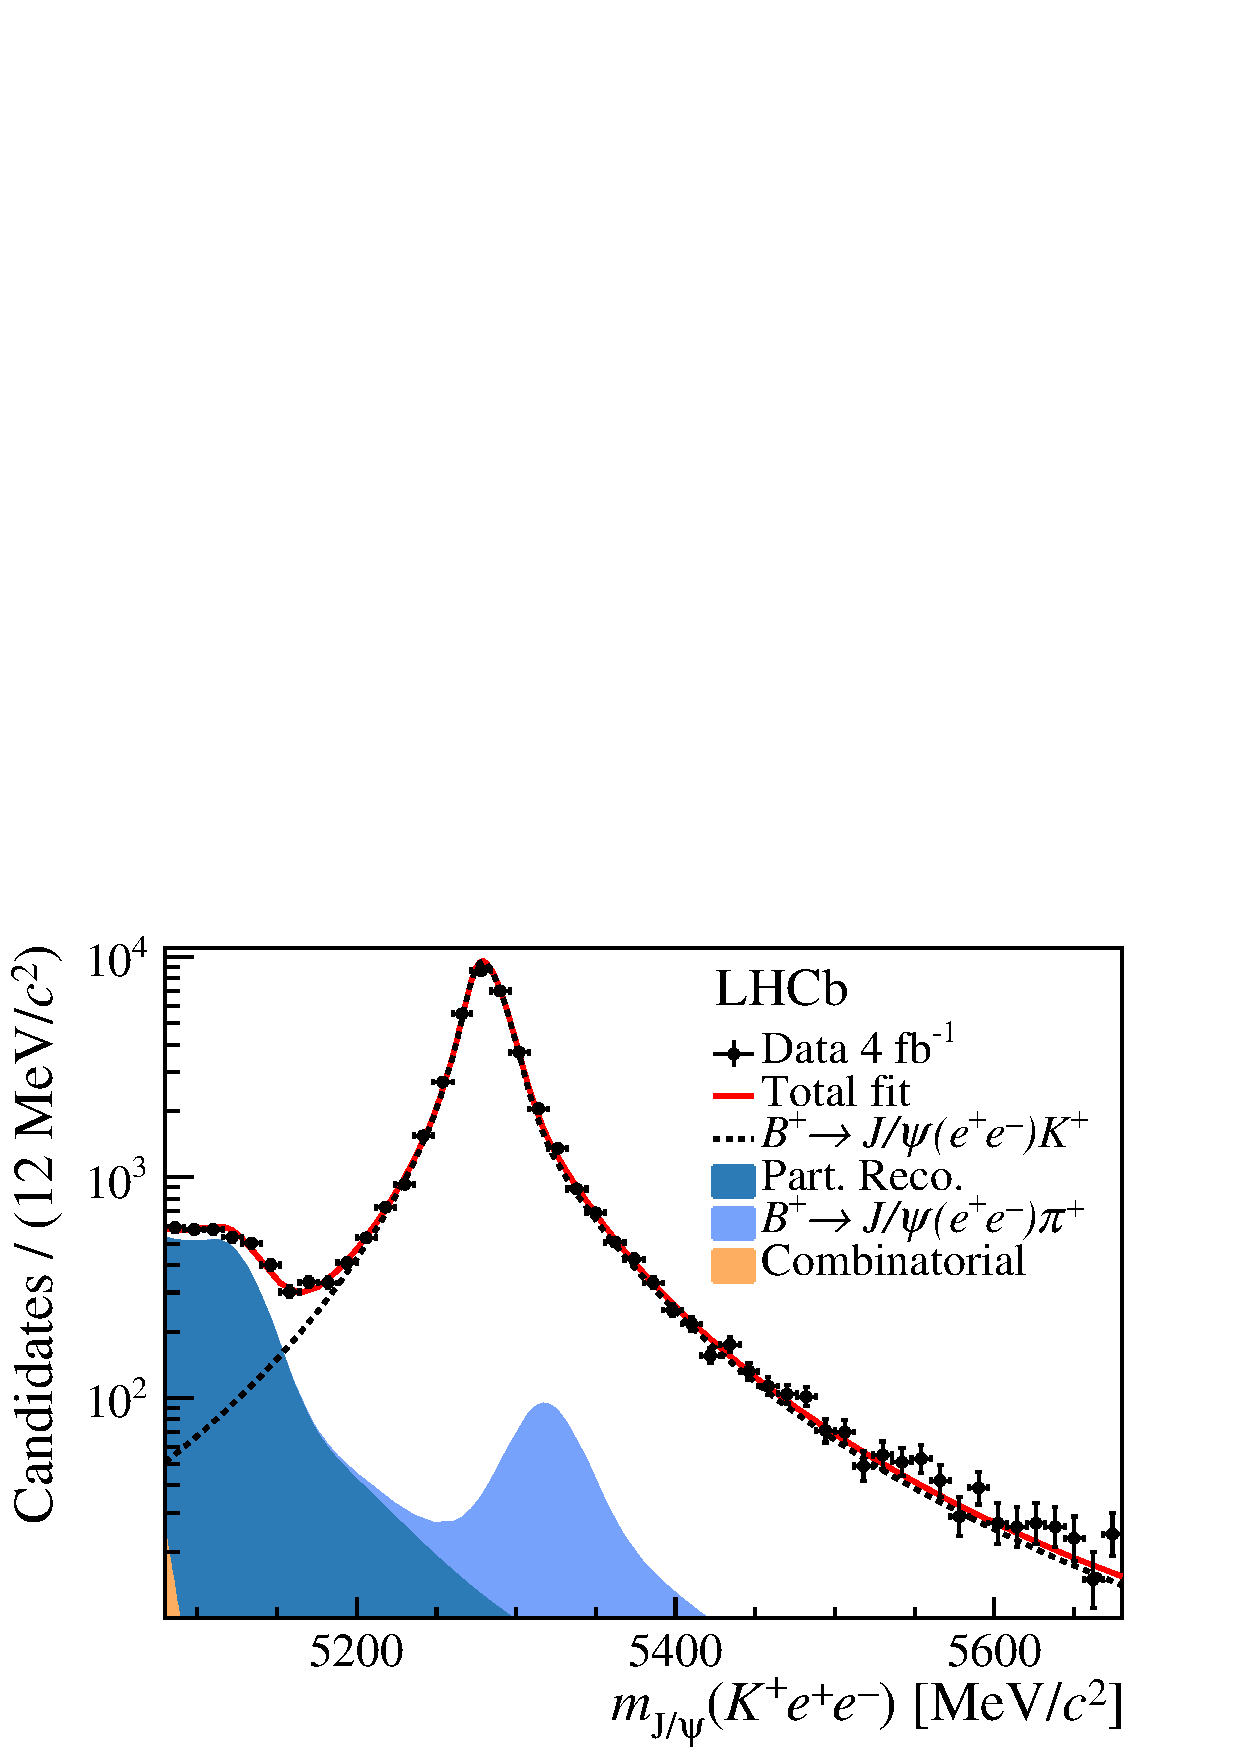
\includegraphics[width=0.45\textwidth]{figures/Fig7f.pdf}
    
    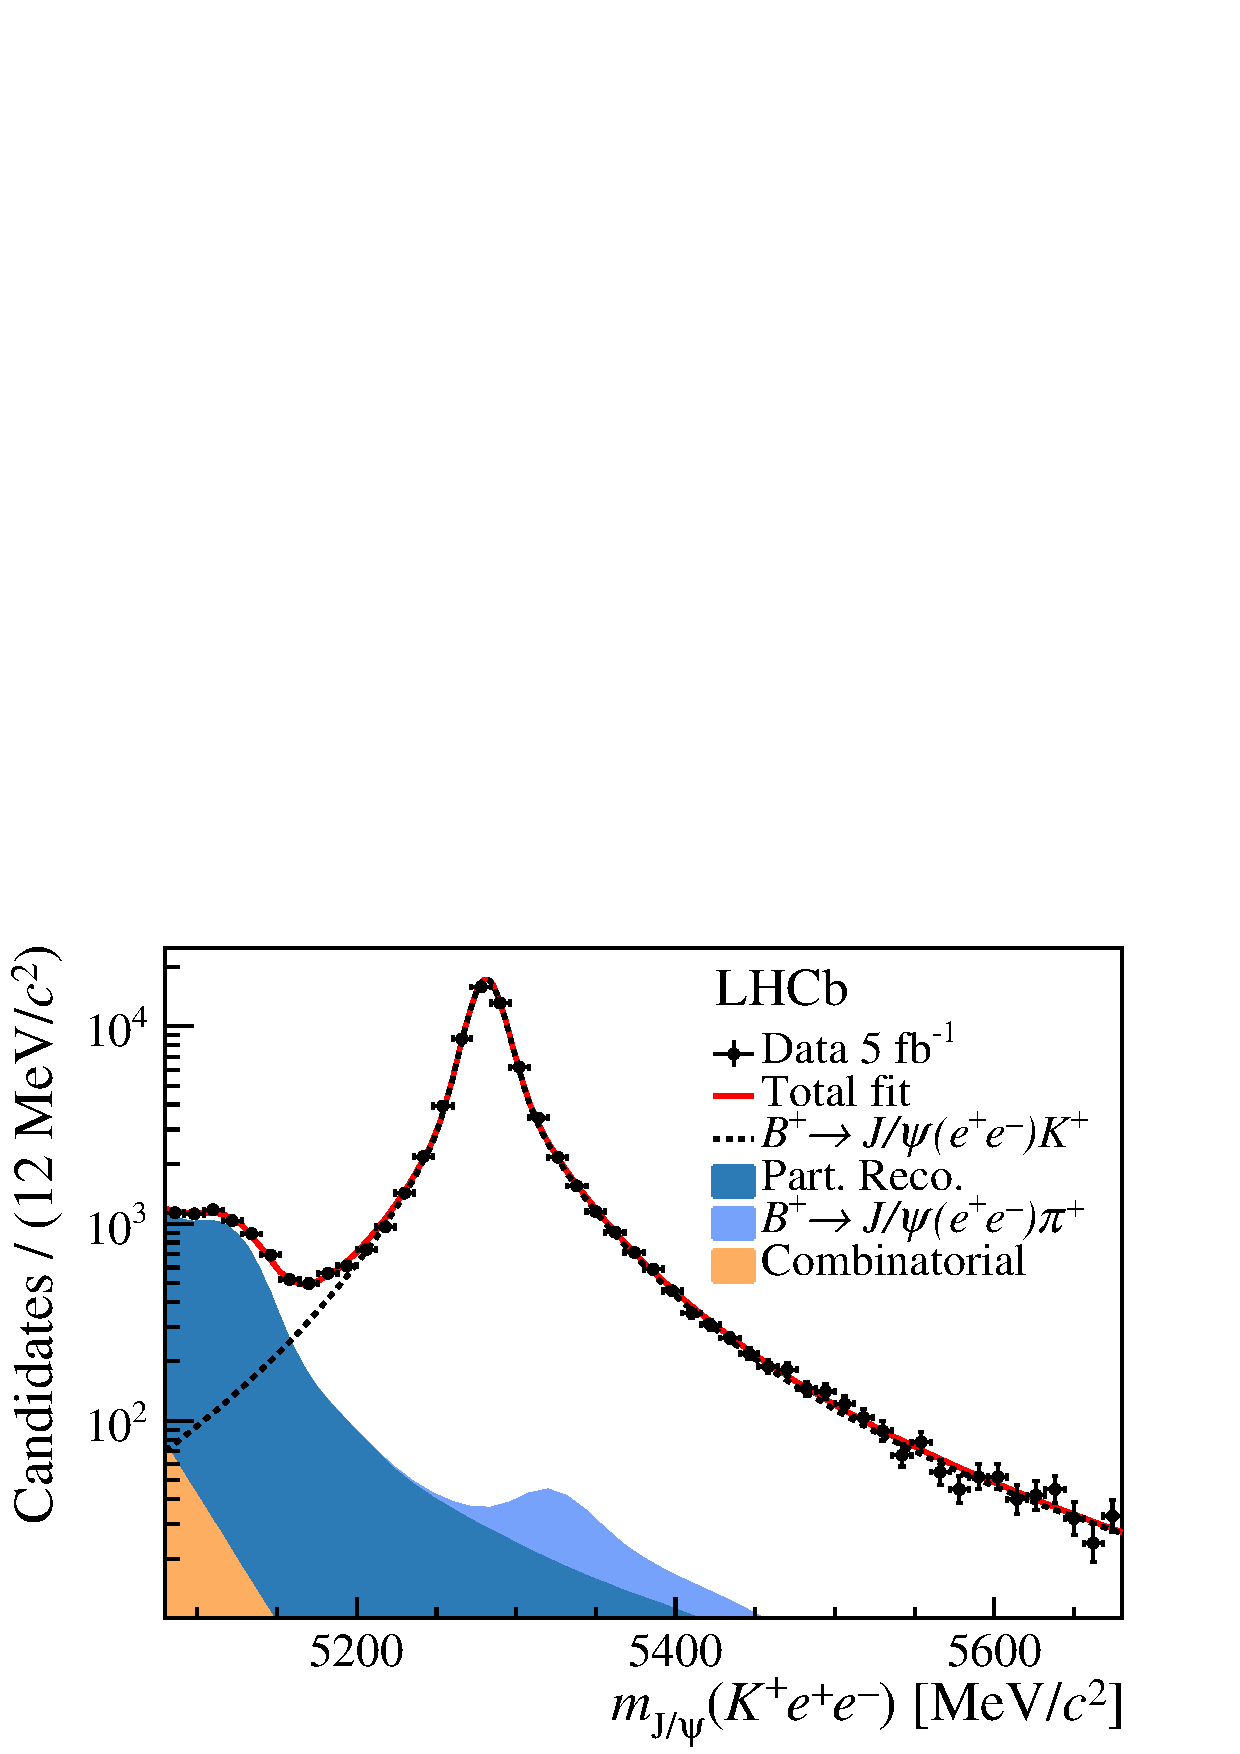
\includegraphics[width=0.45\textwidth]{figures/Fig7g.pdf}
    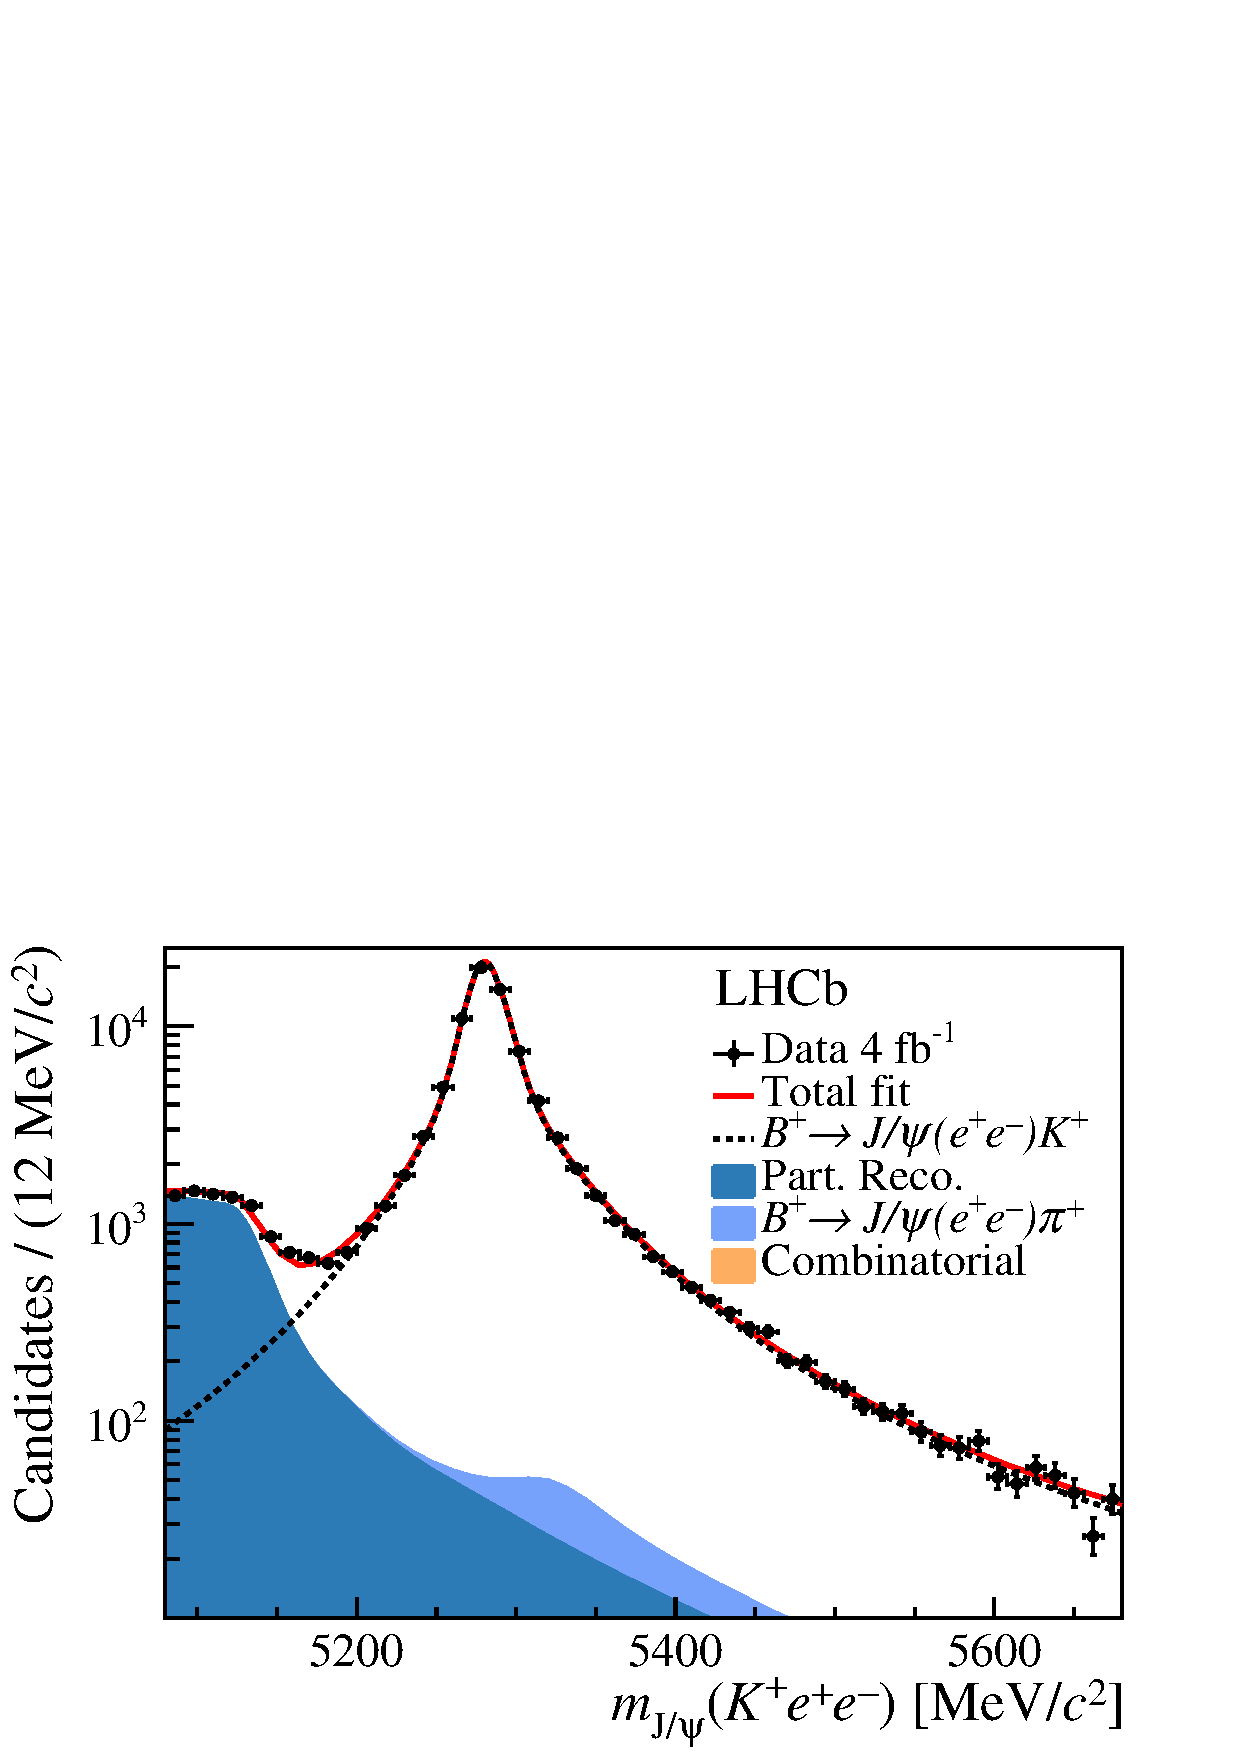
\includegraphics[width=0.45\textwidth]{figures/Fig7h.pdf}
    
    \caption{Candidate invariant mass distributions. Distribution of the invariant mass \mKllconst for resonant candidates in the (left) sample previously analysed~\cite{LHCb-PAPER-2019-009} and (right) the new data sample. The top row shows the fit to the muon modes and the subsequent rows the fits to the electron modes triggered by (second row) one of the electrons, (third row) the kaon and (last row) by other particles in the event. The fit projections are superimposed.
}
    \label{fig:resfits_categories}
\end{figure}


The profile likelihood for the fit to the nonresonant decays is shown in Fig.~\ref{fig:profile_likelihood}. The likelihood is non-Gaussian in the region $\RK>0.95$ due to the comparatively low yield of \BuKee events. 
Following the procedure described in Refs.~\cite{LHCb-PAPER-2019-009, LHCb-PAPER-2017-013}, the p-value is computed by integrating the posterior probability density function for \RK, having folded in the theory uncertainty on the SM prediction, for \RK values larger than the SM  expectation. The corresponding significance in terms of standard deviations is computed using the inverse Gaussian cumulative distribution function for a one-sided conversion.

A test statistic is constructed that is based on the likelihood ratio between two hypotheses with common (null) or different (test) \RK values for the part of the sample analysed previously (7, 8 and part of the 13\tev data) and for the new portion of the 13\tev data. Using pseudoexperiments based on the null hypothesis, the data suggest that the \RK value from the new portion of the data is compatible with that from the previous sample with a p-value of 95\%. Further tests give good compatibility for subsamples of the data corresponding to different trigger categories and magnet polarities.

The departure of the profile likelihood shown in Fig.~\ref{fig:profile_likelihood} from a normal distribution stems from the  definition of \RK. In particular,
in the \RK ratio the denominator is affected by larger statistical uncertainties than the numerator, owing to the larger number of nonresonant muonic signal candidates. However, the intervals of the likelihood distribution are found to be the same when estimated with $1/\RK$ as the fit parameter.


\begin{figure}[!t]
   \begin{center}
      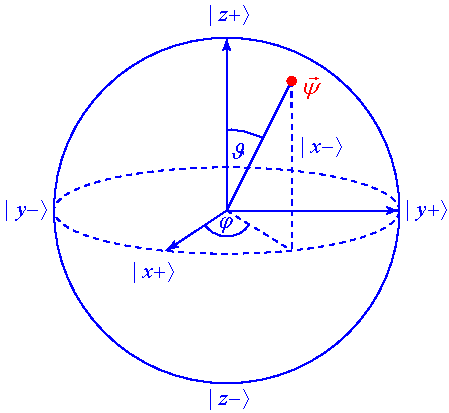
\includegraphics[height=0.25\textheight]{figures/Fig8.pdf}
  \end{center}
     \caption{Likelihood function from the fit to the nonresonant \BuKll candidates profiled as a function of \RK. The extent of the  dark, medium and light blue  regions shows the values allowed for \RK at $1\sigma$, $3\sigma$ and $5\sigma$ levels. The red line indicates the prediction from the SM. }
    \label{fig:profile_likelihood}
\end{figure}



\subsubsection*{Additional cross-checks} 

The \rjpsi single ratio is used to perform a number of additional cross-checks. The distribution of this ratio as a function of the angle between the leptons and the minimum \pt of the leptons is shown in Fig.~\ref{fig:rjpsi_differential1}, together with the spectra expected for the resonant and nonresonant decays.
No significant trend is observed in either \rjpsi distribution. Assuming the deviations observed are genuine mismodelling of the efficiencies, rather than statistical fluctuations, a total shift of \RK at a level less than $0.001$ would be expected due to these effects. This estimate takes into account the spectrum of the relevant variables in the nonresonant decay modes of interest and is compatible with the estimated systematic uncertainties on \RK. Similarly, the variations seen in \rjpsi as a function of all other reconstructed quantities examined are compatible with the systematic uncertainties assigned. In addition, \rjpsi is computed in two-dimensional intervals of reconstructed quantities, as shown in Fig.~\ref{fig:rjpsi_bin}. Again, no significant trend is seen.
 
\begin{figure}[!t]
   \begin{center}
   \begin{overpic}[width=0.45\linewidth,trim={0 0 0 0.5cm}, clip]{figures/Fig9a.pdf}
   \put(50,26){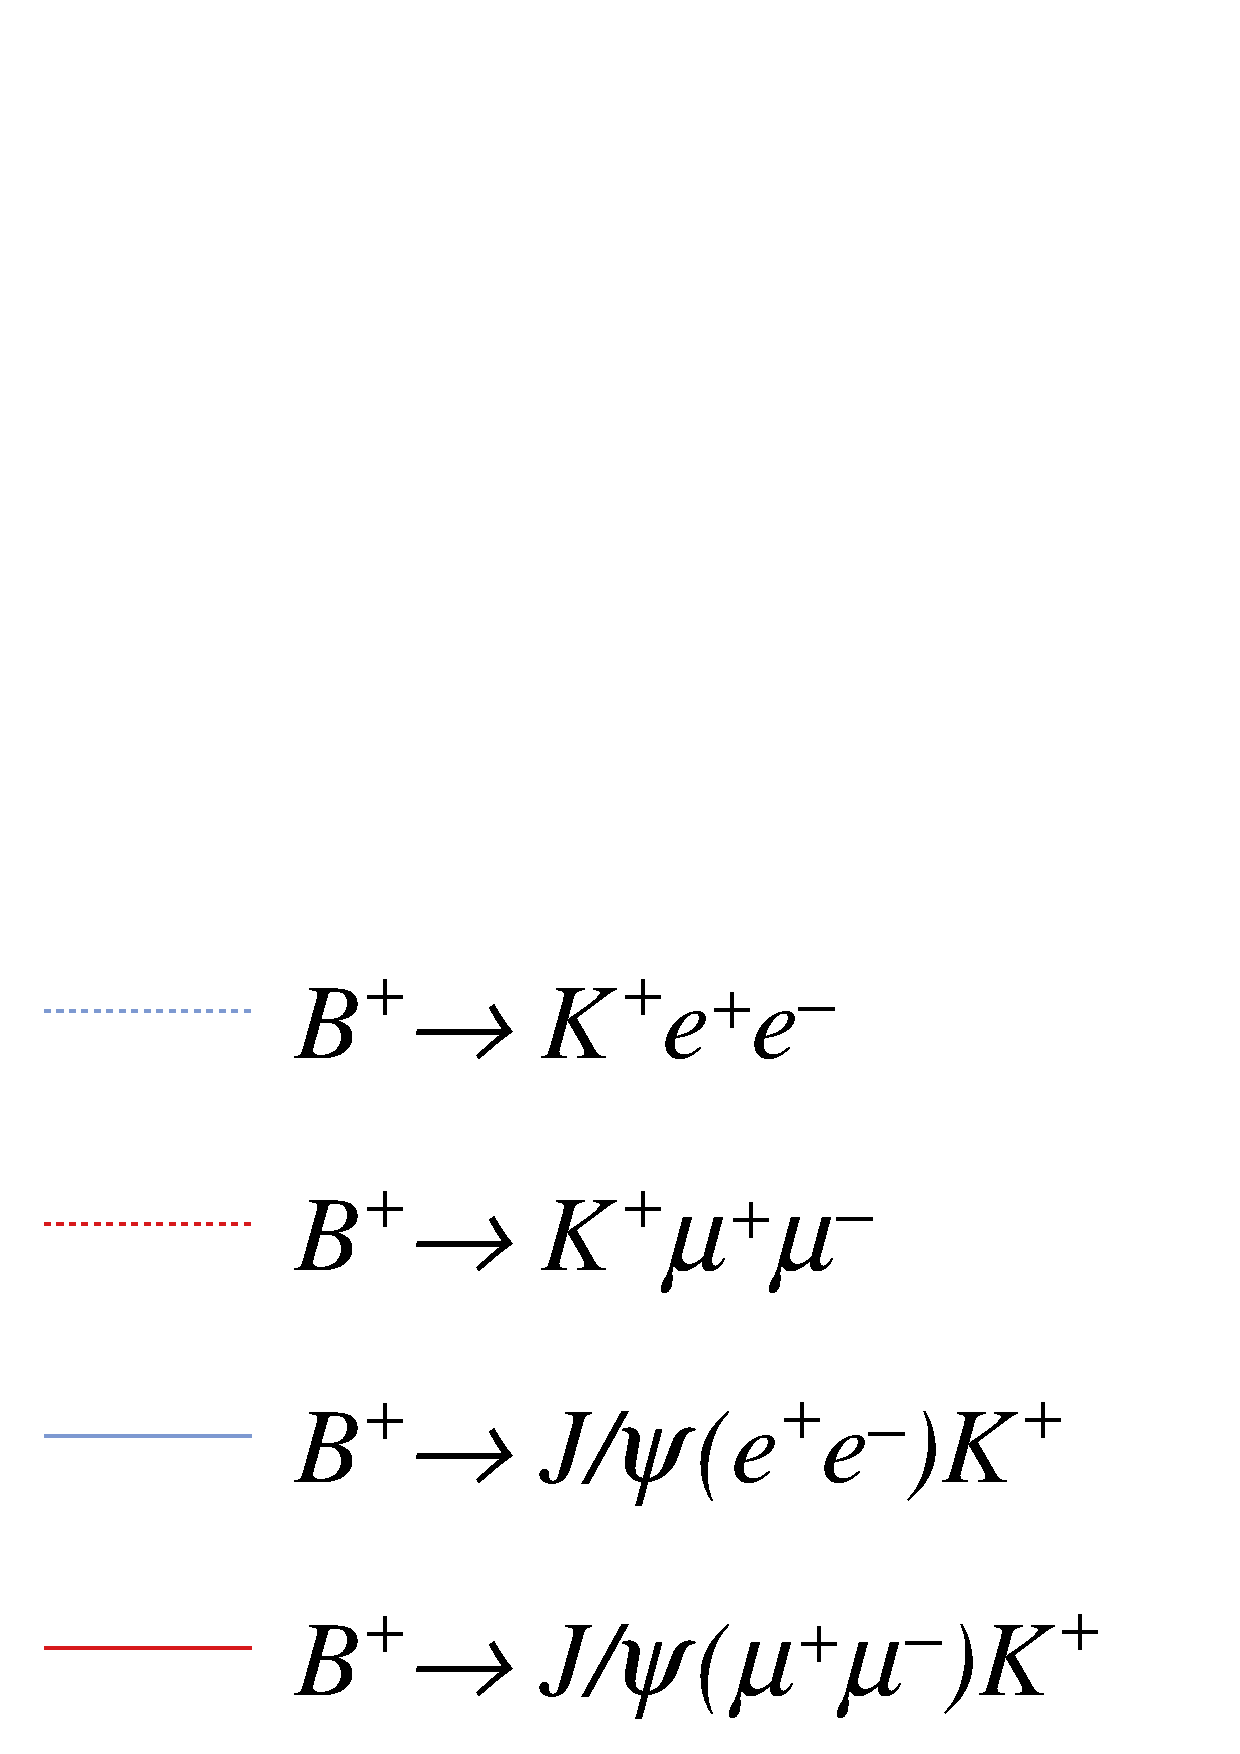
\includegraphics[width=0.2\linewidth]{figures/Fig9e.pdf}}
   \end{overpic}
   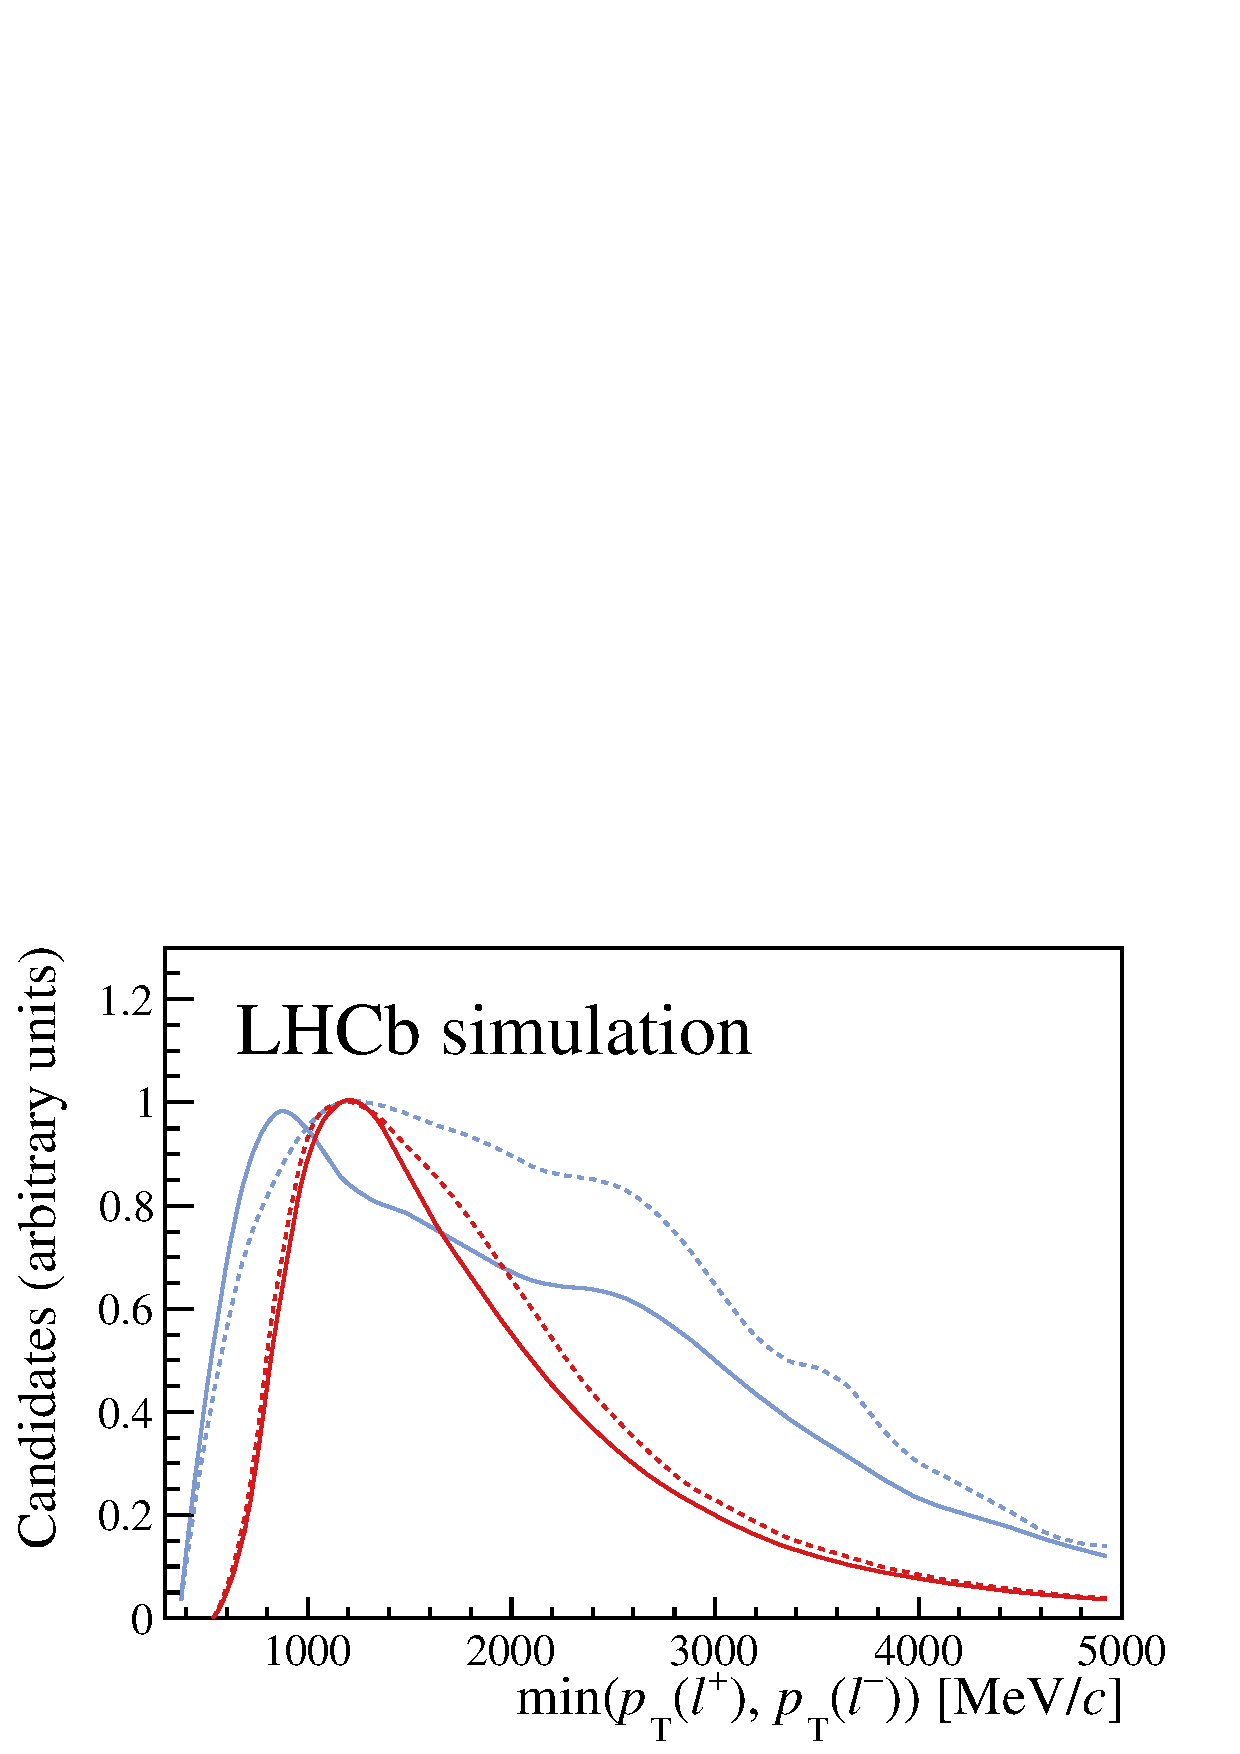
\includegraphics[width=0.45\linewidth,trim={0 0.15cm 0 0}, clip]{figures/Fig9b.pdf}
   
  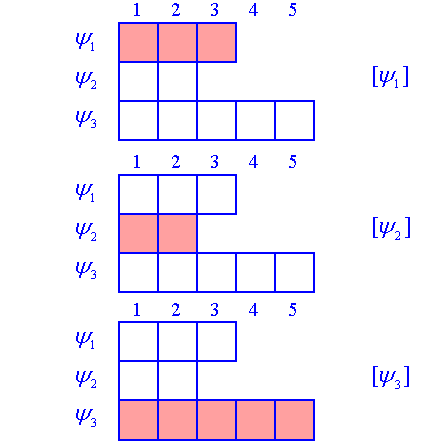
\includegraphics[width=0.45\linewidth,trim={0 0 0 0.5cm}, clip]{figures/Fig9c.pdf}
   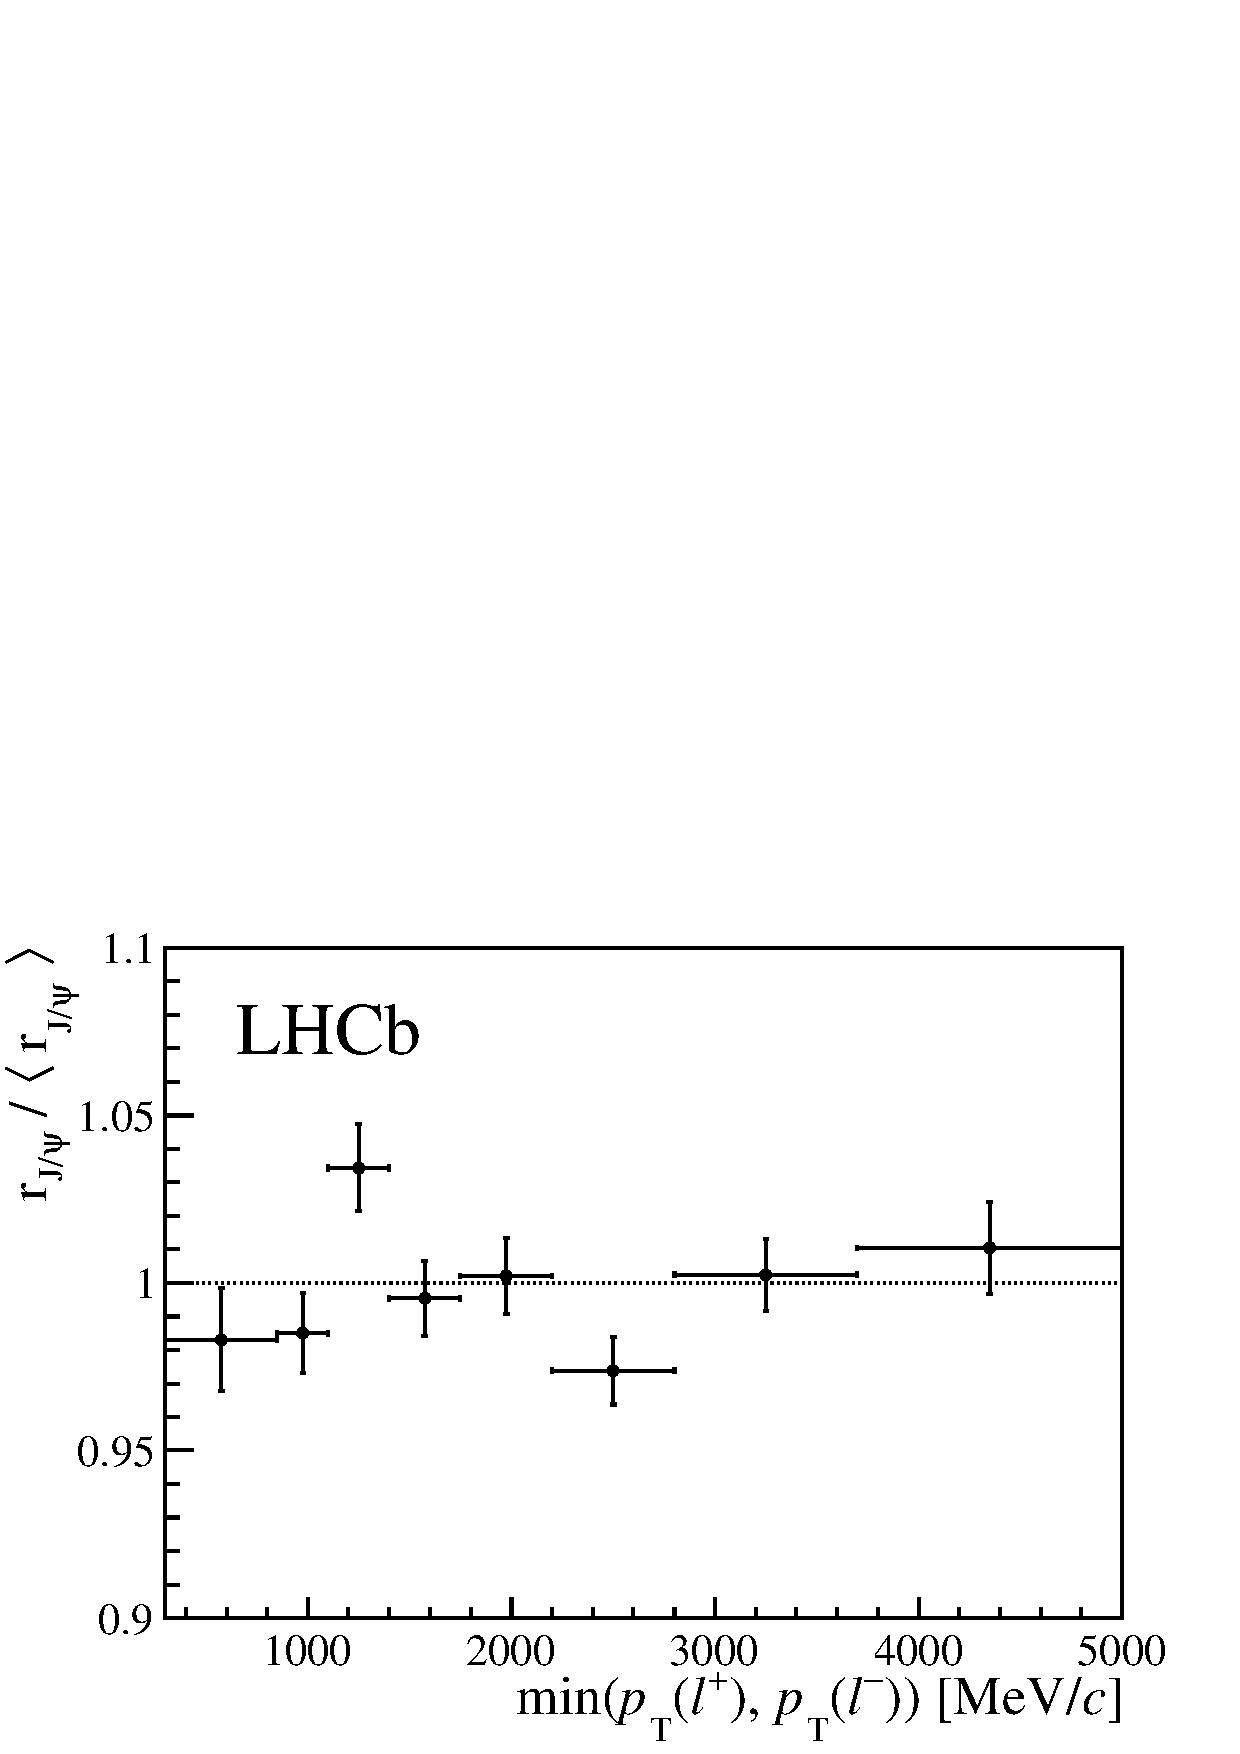
\includegraphics[width=0.45\linewidth,trim={0 0 0 0.5cm}, clip]{figures/Fig9d.pdf}
      \end{center}
     \caption{Differential \rjpsi measurement. (Top) distributions of the reconstructed spectra of (left) the angle between the leptons, and (right) the minimum \pt of the leptons. (Bottom) the single ratio \rjpsi relative to its average value $\left< \rjpsi \right>$ as a function of these variables. In the electron minimum \pt spectra, the structure at 2800\mevc is related to the trigger threshold.}
    \label{fig:rjpsi_differential1}
\end{figure}


\begin{figure}[!htbp]
   \begin{center}
   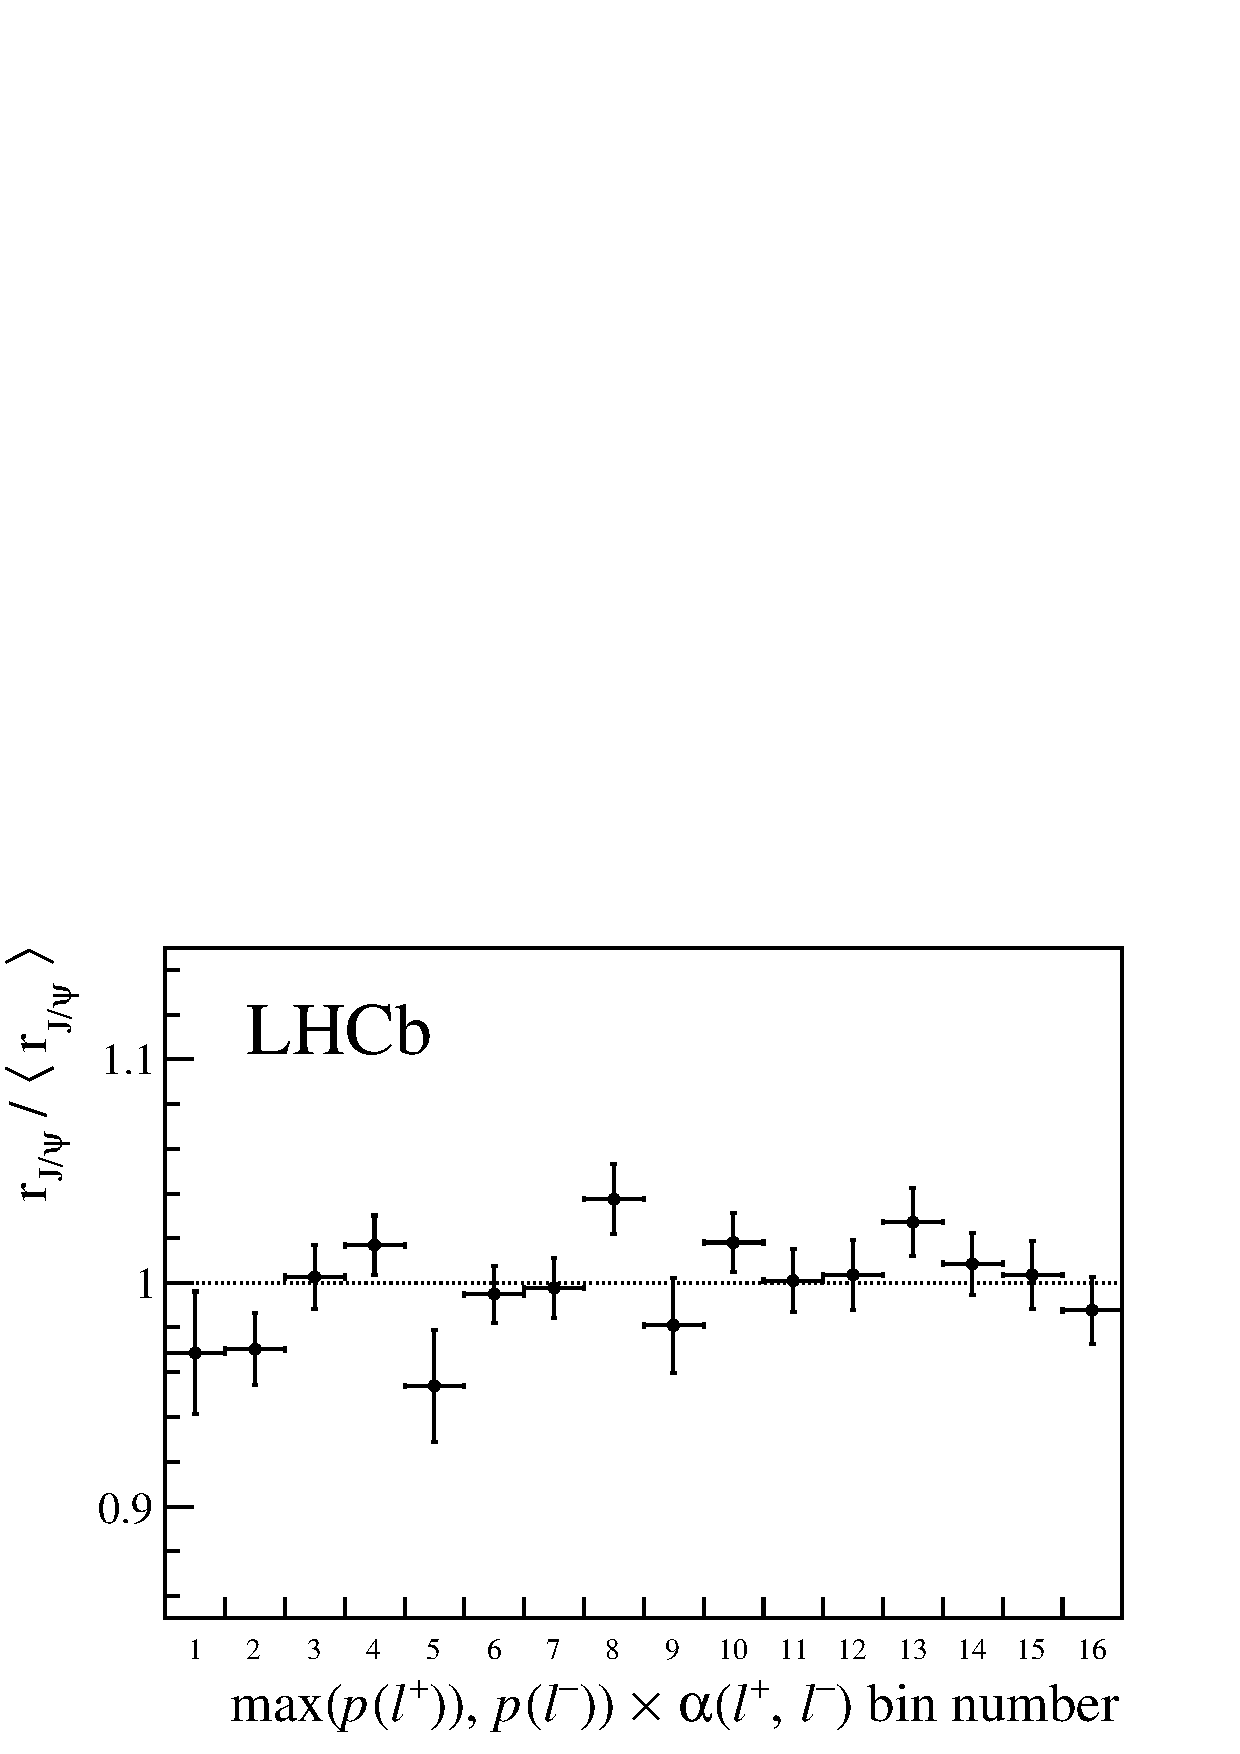
\includegraphics[width=0.45\linewidth]{figures/Fig10a.pdf}
    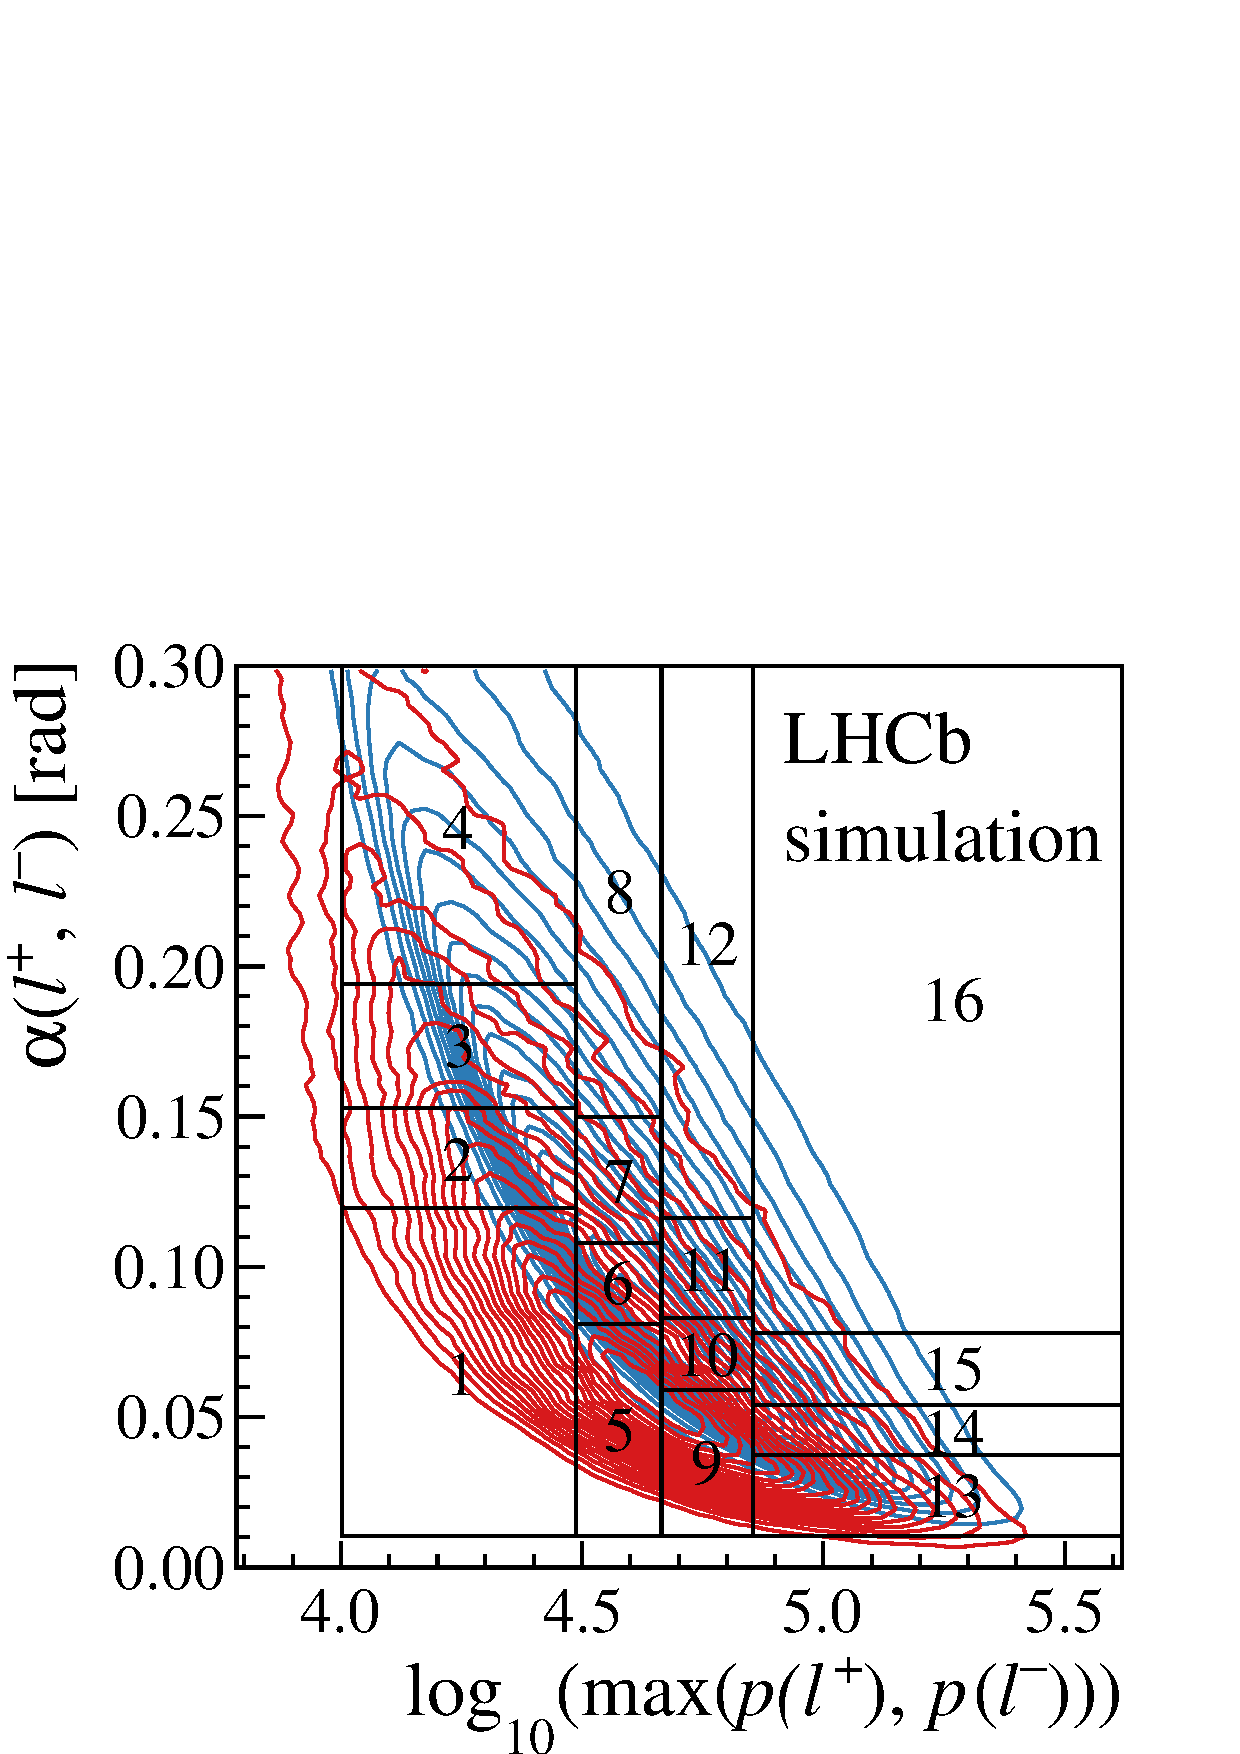
\includegraphics[height=0.32\linewidth]{figures/Fig10b.pdf}
   \end{center}
     \caption{Double differential \rjpsi measurement. (Left) the value of \rjpsi, relative to the average value of \rjpsi, measured in two-dimensional bins of the maximum lepton momentum, $p(l)$, and the opening angle between the two leptons, $\alpha(l^+,l^-)$. (Right) the bin definition in this two-dimensional space together with the
     distribution for \BuKee (\BuJpsiKee) decays depicted as red (blue) contours.}
    \label{fig:rjpsi_bin}
\end{figure}




\subsubsection*{Systematic uncertainties}

The majority of the sources of systematic uncertainty affect the relative efficiencies between nonresonant and resonant decays. These are included in the fit to \RK by allowing the relative efficiency to vary within Gaussian constraints. The width of the constraint is determined by adding the contributions from the different sources in quadrature. Correlations in the systematic uncertainties between different trigger categories and run periods are taken into account. Systematic uncertainties affecting the determination of the signal yield are assessed using pseudoexperiments generated with variations of the fit model. Pseudoexperiments are also used to assess the degree of bias originating from the fitting procedure. The bias is found to be 1\% of the statistical precision, \ie negligible with respect to other sources of systematic uncertainty.

For the nonresonant \BuKee decays, the systematic uncertainties are dominated by the modelling of the signal and background components used in the fit. The effect is at the 1\% level. A significant proportion (0.7\%) of this  uncertainty comes from the limited knowledge of the $K\pi$ spectrum in \BuBdKpiplusee decays. In addition, a 0.2\% systematic uncertainty is assigned for the potential contribution from \BuBdKpipiplusee events. 
A comparable uncertainty to that from the modelling of the signal and background components is induced by the limited sizes of calibration samples. Other sources of systematic uncertainty, such as the calibration of \Bu production kinematics, the trigger calibration and the determination of the particle identification efficiencies, contribute at the few-permille or permille level, depending strongly on the data-taking period and the trigger category. 


% The effect on \RK is at the $\pm0.008$ level. A  comparable uncertainty arises from the limited size of the calibration samples, with negligible contributions from the calibration of \Bu production kinematics and modelling of the selection and particle identification efficiencies. 

The uncertainties on parameters used in the simulation model of the signal decays affect the \qsq distribution and hence the selection efficiency. These uncertainties are propagated to an uncertainty on \RK using predictions from the {\sc{flavio}} software package~\cite{Straub:2018kue} but give rise to a negligible effect. Similarly, the differing \qsq resolution between data and simulation, which alters estimates of the \qsq migration, has negligible impact on the result.

\begin{figure*}[h!]
	\begin{center}
		\hspace*{-.4in}
		\vspace*{-0.3in}
		\begin{tabular}{   c | c  c  c  c  }
			%\hline
			& \large{\textsf{VIDEO 1 }} &\large{\textsf{VIDEO 2}}   &\large{\textsf{VIDEO 3}} &\large{\textsf{VIDEO 4}}      \\ 
			&\vspace{-.1in}&&&\\
			& \large{\textsf{Pure Rotation}} &\large{\textsf{Rotating Hotspot}}   &\large{\textsf{Face-on Disk}} &\large{\textsf{Edge-on Disk}}      \\ \hline
			&\vspace{-.1in}&&&\\
			\multirow{1}{*}[0.9in]{ \rotatebox[origin=t]{90}{\small{\textsf{SINGLE FRAME}} }}
			&
			{{\includegraphics[height=.15\linewidth]{figures/starwarps_results/rotation30/gt/frames/gt_15_colorbar.pdf}} } 
			\multirow{2}{*}[.9in]{ \includegraphics[width=0.06\linewidth]{figures/cbar/vertical_cbar_0to12.pdf} }
			&
			\includegraphics[height=.15\linewidth]{figures/starwarps_results/hotspot100sR2/gt/frames/gt_115_colorbar.pdf} 
			\multirow{2}{*}[.9in]{ \includegraphics[width=0.06\linewidth]{figures/cbar/vertical_cbar_0to16.pdf} }
			&
			\includegraphics[height=.15\linewidth]{figures/starwarps_results/hotakamovie_02/gt/frames/gt_85_colorbar.pdf} 
			\multirow{2}{*}[.9in]{ \includegraphics[width=0.0668\linewidth]{figures/cbar/vertical_cbar_0to4.pdf} }
			&
			\includegraphics[height=.15\linewidth]{figures/starwarps_results/hotakamovie_45/gt/frames/gt_63_colorbar.pdf} 
			\multirow{2}{*}[.9in]{ \includegraphics[width=0.06\linewidth]{figures/cbar/vertical_cbar_0to8.pdf} }
			\\
			\multirow{1}{*}[0.7in]{ \rotatebox[origin=t]{90}{\small{\textsf{MEAN}} }}
			&
			{{\includegraphics[height=.15\linewidth]{figures/starwarps_results/rotation30/gt/pavgimg_colorbar.pdf}} } \hspace{.55in} &
			\includegraphics[height=.15\linewidth]{figures/starwarps_results/hotspot100sR2/gt/pavgimg_colorbar.pdf} \hspace{.55in} &
			\includegraphics[height=.15\linewidth]{figures/starwarps_results/hotakamovie_02/gt/pavgimg_colorbar.pdf} \hspace{.55in} &
			\includegraphics[height=.15\linewidth]{figures/starwarps_results/hotakamovie_45/gt/pavgimg_colorbar.pdf} \hspace{.55in}
			\\ \hline
			&\vspace{-.1in}&&&\\
			\multirow{1}{*}[0.9in]{ \rotatebox[origin=t]{90}{\small{\textsf{STD. DEVIATION}} }}
			& \hspace{0.01in}
			{{\includegraphics[height=.147\linewidth]{figures/starwarps_results/rotation30/gt/stdevimg_noaxis_r2.pdf}} } \hspace{.59in} & 
			
			\hspace{0.01in}
			 \includegraphics[height=.147\linewidth]{figures/starwarps_results/hotspot100sR2/gt/stdevimg_noaxis_r2.pdf}  \hspace{.59in} &
			
			\hspace{-0.01in} \includegraphics[height=.147\linewidth]{figures/starwarps_results/hotakamovie_02/gt/stdevimg_noaxis_r2.pdf}  \hspace{.55in} & 
			\hspace{-0.01in}
			\includegraphics[height=.147\linewidth]{figures/starwarps_results/hotakamovie_45/gt/stdevimg_noaxis_r2.pdf} \hspace{.55in} 
			\\
		\end{tabular}
		\vspace{.1in}
		\caption{{\bf Ground truth videos:} The four ground truth sequences used to demonstrate results. We show a single frame from each sequence, the mean frame, and the spatial standard deviation of flux density. Video 1 consists of a $160 \mu$-arcsecond image~\cite{avery} that rotates $180^{\circ}$ over the course of a 12 hour observation (24 hour rotational period). Video 2 is a $120 \mu$-arcsecond view of an edge-on black hole disk with a rotating ``hot spot" predicted by~\cite{Broderick_Loeb_2006} with a rotational period of 2.78 hours. Video 3 and 4 are generated using a model of a black hole observed face on and at a $45^{\circ}$ inclination with a $160 \mu$-arcsecond field of view~\cite{Shiokawa_2013}. They assume a spin of 0.9375 with an Innermost Stable Circular Orbit (ISCO) rotational period of 8.96 minutes. The specified FOV and colormaps for the single frame and mean images are used for each corresponding video throughout the remainder of the paper. }
		%video 1: 1.2 max val
		%video 2: 1.6 maxval
		%video 3: .4 maxval
		%video 4: .8 maxval
		\label{fig:groundtruth}
	\end{center}
		\vspace{-.2in}
\end{figure*}

\vspace{-.07in}
\section{Dynamic Imaging Results}
\label{sec:results}

As data from the EHT 2017 campaign is yet to be released, in this section we demonstrate our method on synthetic EHT data and real data from the Very Long Baseline Array (VLBA). Additional results can be seen in the supplemental document and video. The StarWarps algorithm has been implemented as part of the publicly available python \texttt{eht-imaging}\footnote{\url{https://github.com/achael/eht-imaging}} library~\cite{andrew}.

\vspace{-.2in}
\subsection{Synthetic Data Generation} 

We demonstrate our algorithm on synthetic data generated from four different sequences of time-varying sources. These sequences include two realistic fluid simulations of a black hole accretion disk for different observing orientations~\cite{Shiokawa_2013}, a realistic sequence of a ``hot spot" rotating around a black hole~\cite{Broderick_Loeb_2006}, and a toy sequence evolving with pure rotation. The field of view of each sequence ranges from 120 to 160 $\mu$-arcseconds. A still frame from each sequence is shown in Figure~\ref{fig:groundtruth}. To help give a sense of the variation in each sequence, the figure also displays the mean and standard deviation of flux density. We refer to these sequences by their video number, indicated in the figure. 



In order to demonstrate the quality of results under various observing conditions, VLBI observations of SgrA* at 1.3 mm (230 GHz) are simulated assuming
 three different telescope arrays.  The first array, EHT2017, consists of the 8 telescopes at 6 distinct locations that were used to collect measurements for the Event Horizon Telescope in the spring of 2017. The uv-coverage for this array can be seen in Figure~\ref{fig:staticimaging}. The second array, EHT2017+, augments the EHT2017 array with 3 potential additions to the EHT: Plateau de Bure (PDB), Haystack (HAY), and Kitt Peak (KP) Observatory. 
Details on telescopes used in the EHT2017 and EHT2017+ array are shown in Table~\ref{tab:telescopes}.  
The third array, FUTURE, consists of 9 additional telescopes. The uv-coverage of these latter two arrays, along with a colorbar indicating the time of each measurement, is shown in Figures~\ref{fig:uvcov2}. 
%Details on telescopes used in these arrays are shown in the supplemental material.


Visibility measurements are generated using the python \texttt{eht-imaging} library~\cite{andrew}. %assuming a 4 GHz bandwidth with a 100 second integration time. 
Realistic thermal noise, resulting from a bandwidth ($\Delta \nu$) of 4 GHz and a 100 second integration time ($t_{\rm int}$), is introduced on each visibility. The standard deviation of thermal noise is given by
\begin{align}
\sigma = \frac{1}{0.88} \sqrt{\frac{\mbox{SEFD}_1 \times \mbox{SEFD}_2 }{2 \times \Delta \nu \times t_{\rm int} } },
\label{eq:thermal}
\end{align}

\noindent{for System Equivalent Flux Density (SEFD) of the two telescopes corresponding to each visibility\footnote{The factor of 1/0.88 is due to information loss due to recording 2-bit quantized data-streams at each telescope~\cite{TMS}.}~\cite{taylor1999synthesis}.  %, and using bandwidth $\Delta \nu$ and integration time $t_{int}$.}
% in the absense of atmospheric error
%Atmospheric phase error is also introduced into measurements using the \texttt{eht-imaging} library. 
Random station-based atmospheric phases drawn from a uniform distribution at each time step are introduced into measurements using the \texttt{eht-imaging} library. 
In Videos 2-4 a set of measurements is sampled every 5 minutes over a roughly 14 hour duration, resulting in 173 time steps. In Video 1 only 30 time steps are measured over a 12 hour duration. 
}


\begin{figure}[h!]
	\centering
	%{\includegraphics[height=.28\linewidth]{figures/uvcoverage/uv_eht2017.pdf}}
	{\includegraphics[height=.38\linewidth]{figures/uvcoverage/uv_ehtfuture2_2.pdf}}
	{\includegraphics[height=.38\linewidth]{figures/uvcoverage/uv_ehtfuture1_2.pdf}}
	\caption{{\bf Time-varying uv-coverage:} The uv-coverage for EHT2017+ and FUTURE arrays when observing SgrA∗. The uv-coverage for the EHT2017 array can be seen in Figure~\ref{fig:staticimaging}. 
		Baselines are colored by the time of each observation relative to the start time, indicated by the colorbar to the right.}
	\label{fig:uvcov2}

\end{figure}


\begin{table}[!t]
	\begin{center}
		\caption{EHT 2017 Station Parameters}
		\label{tab::eht_station}
		\begin{tabular}{ccc}
 Telescope & Location & SEFD (Jy) \\ \hline
 ALMA & Chile & 110 \\ 
 APEX & Chile & 22000 \\ 
 LMT & Mexico & 560 \\
 SMT & Arizona & 11900 \\ 
 SMA & Hawaii & 4900 \\
 JCMT & Hawaii & 4700 \\ 
 PV & Spain & 2900 \\ 
 SPT & South Pole & 1600 \\ \hline
 PDB* & France & 1600 \\ 
 HAY* & Massachusetts & 2500 \\ 
 KP* & Arizona & 2500 \\ \hline
		\end{tabular}\\
	\end{center}
	\bigskip
	\footnotesize{The location and SEFD of each telescope in the EHT2017 and EHT2017+ arrays. These parameters and locations were used to generate the uv-trajectories in frequency space shown in Figure~\ref{fig:staticimaging} and~\ref{fig:uvcov2}. Telescope names followed by a star (*) were not included in the EHT2017 array.}
	\label{tab:telescopes}
	\vspace{-0.3in}
\end{table}



%\begin{table}[h!]
%\begin{center}
%\begin{tabular}{ c c c }
% Telescope & Location & SEFD (Jy) \\ \hline
% ALMA & Chile & 110 \\ 
% APEX & Chile & 22000 \\ 
% LMT & Mexico & 560 \\
% SMT & Arizona & 11900 \\ 
%SMA & Hawaii & 4900 \\
%JCMT & Hawaii & 4700 \\ 
% PV & Spain & 2900 \\ 
% SPT & South Pole & 1600 \\ \hline
% PDB* & France & 1600 \\ 
% HAY* & Massachusetts & 2500 \\ 
%  KP* & Arizona & 2500 \\ \hline
%\end{tabular}
%\end{center}
%\caption{ The location and SEFD of each telescope in the EHT2017 and EHT2017+ arrays. These parameters and locations were used to generate the uv-trajectories in frequency space shown in Figure~\ref{fig:staticimaging} and~\ref{fig:uvcov2}. Telescope names followed by a star (*) were not included in the EHT2017 array. }
%\label{tab:telescopes}
%\vspace{-0.3in}
%\end{table}

\vspace{-.1in}
\subsection{Static Evolution Model (No Warp)}
\label{sec:nomotionresults}

We first demonstrate results of our method under a static evolution model. In this case, we fix parameters $\theta$ such that $A=\mathds{1}$. This assumes that there is no global motion under a persistent warp field, but only perturbations around a fairly static scene. Despite this incorrect assumption (especially in Videos 1 and 2), this simple model results in reconstructions that surpass the state-of-the-art methods, and recovers distinctive structures that appear in the underlying source images. 


\subsubsection{Synthetic Data Result Comparison}

\begin{figure*}
	\begin{center}
	%	\vspace{-0.5in}
		%\hspace*{-2.3cm}
		\setlength{\tabcolsep}{3pt}
		
		\hspace{-0.5in}\normalsize{\textsf{BLURRED TRUE MEAN}}  \hspace{5.5cm} \normalsize{\textsf{NORMALIZED RMSE}} 
		\vspace{0.1in}
		
		
%	\begin{tabular}{ c " c}
%		VIDEO 1& VIDEO 2 \\ \thickhline
%		& \vspace{-.1in} \\
%		VIDEO 3 & VIDEO 4
%	\end{tabular}
%	\qquad
%		\begin{tabular}{ c " c}
%		{{\includegraphics[height=.1\linewidth]{figures/starwarps_results/rotation30/gt/frames/gt_15_blurredbeam75_noaxis.pdf}} } & {{\includegraphics[height=.1\linewidth]{figures/starwarps_results/hotspot100sR2/gt/frames/gt_115_blurredbeam75_noaxis.pdf}} } \\ \thickhline
%		& \vspace{-.1in} \\
%	{{\includegraphics[height=.1\linewidth]{figures/starwarps_results/hotakamovie_02/gt/frames/gt_85_blurredbeam75_noaxis.pdf}} } & {{\includegraphics[height=.1\linewidth]{figures/starwarps_results/hotakamovie_45/gt/frames/gt_63_blurredbeam75_noaxis.pdf}} }
%		\end{tabular}
						\begin{tabular}{ c " c}
							\hspace{-.06in} \textsf{Video 1} & \hspace{-.06in} \textsf{Video 2} \\
							{{\includegraphics[height=.1\linewidth]{figures/starwarps_results/rotation30/gt/pavgImg_blurredbeam75_noaxis.pdf}} } & {{\includegraphics[height=.1\linewidth]{figures/starwarps_results/hotspot100sR2/gt/pavgImg_blurredbeam75_noaxis.pdf}} } \\ \thickhline
							& \vspace{-.1in} \\
							\hspace{-.06in} \textsf{Video 3} & \hspace{-.06in} \textsf{Video 4} \\
							{{\includegraphics[height=.1\linewidth]{figures/starwarps_results/hotakamovie_02/gt/pavgImg_blurredbeam75_noaxis.pdf}} } & {{\includegraphics[height=.1\linewidth]{figures/starwarps_results/hotakamovie_45/gt/pavgImg_blurredbeam75_noaxis.pdf}} }
						\end{tabular}	
	%	\qquad	
		\qquad
		\begin{tabular}{ r | c | c | c | c " c | c | c | c}
			& \rotatebox[origin=t]{90}{\small{\textsf{EHT 2017}} } \rotatebox[origin=t]{90}{\small{\textsf{NO ATM.}} }  & \rotatebox[origin=t]{90}{\small{\textsf{EHT 2017}} } \rotatebox[origin=t]{90}{\small{\textsf{ATM.}} } & \rotatebox[origin=t]{90}{\small{\textsf{EHT 2017+}} } \rotatebox[origin=t]{90}{\small{\textsf{ATM.}} } &\rotatebox[origin=t]{90}{\small{\textsf{FUTURE}} } \rotatebox[origin=t]{90}{\small{\textsf{ATM.}} } & \rotatebox[origin=t]{90}{\small{\textsf{EHT 2017}} } \rotatebox[origin=t]{90}{\small{\textsf{NO ATM.}} }  & \rotatebox[origin=t]{90}{\small{\textsf{EHT 2017}} } \rotatebox[origin=t]{90}{\small{\textsf{ATM.}} } & \rotatebox[origin=t]{90}{\small{\textsf{EHT 2017+}} } \rotatebox[origin=t]{90}{\small{\textsf{ATM.}} } &\rotatebox[origin=t]{90}{\small{\textsf{FUTURE}} } \rotatebox[origin=t]{90}{\small{\textsf{ATM.}} }  \\ \hline
			{\small{\textsf{StarWarps Mean} } } & {\bf {0.67} }& {\bf {0.65}} & {\bf {0.55} }&  {\bf {0.55}}& {\bf {0.74}} & {\bf {0.73} }& {\bf {0.73}} &  0.71 \\ 
				\cite{freek} & 1.05  & 0.82 & 0.73  & 0.68 &  0.98 & 1.21 & 0.99 & 0.35 \\ 
				\cite{andrew} & 0.79 & 0.80 & 0.73 & 0.63 & 0.83& 1.05 & 0.81 & {\bf 0.23}  \\  \thickhline
				\small{\textsf{StarWarps Mean} } & {\bf 0.32} & {\bf 0.55} & 0.67 & {\bf 0.36} & {\bf 0.34} & {\bf 0.44} & {\bf 0.23} & {\bf 0.31} \\
				\cite{freek} & 0.93 & 0.90 & {\bf 0.53} & 0.51 & 0.84 & 0.75 & 1.02 & 0.61 \\
				\cite{andrew} &0.84 & 0.85 & 0.71 &  0.39  & 0.60 & 0.50 & 0.60 & 0.47
			\end{tabular}

		\vspace{0.4in}
		
		\hspace*{-1.3cm}
		\begin{tabular}{  c c | c  c  c  c "  c  c  c  c  }
			%\hline
			& \small{\textsf{Array:}} &\small{\textsf{EHT 2017}}   &\small{\textsf{EHT 2017 }} &\small{\textsf{EHT2017+}}    &\small{\textsf{FUTURE}}    &\small{\textsf{EHT 2017}}   &\small{\textsf{EHT 2017 }} &\small{\textsf{EHT2017+}}    &\small{\textsf{FUTURE}}     \\ 
			&\vspace{-.1in} & & & & & & & &\\
			& \small{\textsf{Error:}} &\small{\textsf{NO ATM.}}   &\small{\textsf{ATM.}} &\small{\textsf{ATM.}}    &\small{\textsf{ATM.}}  &\small{\textsf{NO ATM.}}   &\small{\textsf{ATM.}} &\small{\textsf{ATM.}}    &\small{\textsf{ATM.}}   \\ \hline
%			&\vspace{-.1in} & & & & & & & &\\
%			\multirow{2}{*}[0.2in]{ \rotatebox[origin=t]{90}{\small{\textsf{StarWarps}} }}   \hspace{-0.3in} & \multirow{1}{*}[0.5in]{ \rotatebox[origin=t]{90}{\small{\textsf{FRAME}} }}
%			&
%			{{\includegraphics[height=.1\linewidth]{figures/starwarps_results/rotation30/eht2017_100_visibility/nomotion/frames/mean_noaxis_15.pdf}} } &
%			\includegraphics[height=.1\linewidth]{figures/starwarps_results/rotation30/eht2017_100_amp-bispectrum/nomotion/frames/mean_noaxis_15.pdf} &
%			\includegraphics[height=.1\linewidth]{figures/starwarps_results/rotation30/ehtfuture2_100_amp-bispectrum/nomotion/frames/mean_noaxis_15.pdf} &
%			\includegraphics[height=.1\linewidth]{figures/starwarps_results/rotation30/ehtfuture1_100_amp-bispectrum/nomotion/frames/mean_noaxis_15.pdf}  
%			&
%			{{\includegraphics[height=.1\linewidth]{figures/starwarps_results/hotspot100sR2/eht2017_100_visibility/nomotion/frames/mean_noaxis_115.pdf}} } &
%			\includegraphics[height=.1\linewidth]{figures/starwarps_results/hotspot100sR2/eht2017_100_amp-bispectrum/nomotion/frames/mean_noaxis_115.pdf} &
%			\includegraphics[height=.1\linewidth]{figures/starwarps_results/hotspot100sR2/ehtfuture2_100_amp-bispectrum/nomotion/frames/mean_noaxis_115.pdf} &
%			\includegraphics[height=.1\linewidth]{figures/starwarps_results/hotspot100sR2/ehtfuture1_100_amp-bispectrum/nomotion/frames/mean_noaxis_115.pdf} \\
			&\vspace{-.1in} & & & & & & & &\\
			 \multirow{2}{*}[0.6in]{ \rotatebox[origin=t]{90}{\small{\textsf{StarWarps}} }}   \hspace{-0.3in} &	\multirow{1}{*}[0.45in]{ \rotatebox[origin=t]{90}{\small{\textsf{Mean}} }}
			&
			{{\includegraphics[height=.1\linewidth]{figures/starwarps_results/rotation30/eht2017_100_visibility/nomotion/pavgimg_noaxis.pdf}} } &
			\includegraphics[height=.1\linewidth]{figures/starwarps_results/rotation30/eht2017_100_amp-bispectrum/nomotion/pavgimg_noaxis.pdf} &
			\includegraphics[height=.1\linewidth]{figures/starwarps_results/rotation30/ehtfuture2_100_amp-bispectrum/nomotion/pavgimg_noaxis.pdf} &
			\includegraphics[height=.1\linewidth]{figures/starwarps_results/rotation30/ehtfuture1_100_amp-bispectrum/nomotion/pavgimg_noaxis.pdf} 
			&
			{{\includegraphics[height=.1\linewidth]{figures/starwarps_results/hotspot100sR2/eht2017_100_visibility/nomotion/pavgimg_noaxis.pdf}} } &
			\includegraphics[height=.1\linewidth]{figures/starwarps_results/hotspot100sR2/eht2017_100_amp-bispectrum/nomotion/pavgimg_noaxis.pdf} &
			\includegraphics[height=.1\linewidth]{figures/starwarps_results/hotspot100sR2/ehtfuture2_100_amp-bispectrum/nomotion/pavgimg_noaxis.pdf} &
			\includegraphics[height=.1\linewidth]{figures/starwarps_results/hotspot100sR2/ehtfuture1_100_amp-bispectrum/nomotion/pavgimg_noaxis.pdf} 
			\\   \hline
			&\vspace{-.1in} & & & & & & & &\\
			\multirow{2}{*}[0.6in]{ \rotatebox[origin=t]{90}{\small{\textsf{MEM \& TV Regularization}} }}  \hspace{-0.3in} & \multirow{1}{*}[0.4in]{ \rotatebox[origin=t]{90}{\small{\textsf{\cite{freek}}} }}
			&
			{{\includegraphics[height=.1\linewidth]{figures/freeksmoothingresults/im_vis_rotation30_tint100_eht2017_directim_maxit100_it0.pdf}} } &
			\includegraphics[height=.1\linewidth]{figures/freeksmoothingresults/im_apar_rotation30_tint100_eht2017_directim_maxit100_it0.pdf} &
			\includegraphics[height=.1\linewidth]{figures/freeksmoothingresults/im_apar_rotation30_tint100_ehtfuture2_directim_maxit100_it0.pdf} &
			\includegraphics[height=.1\linewidth]{figures/freeksmoothingresults/im_apar_rotation30_tint100_ehtfuture1_directim_maxit100_it0.pdf} 
			&
			{{\includegraphics[height=.1\linewidth]{figures/freeksmoothingresults/im_vis_hotspot100sR2_tint100_eht2017_directim_maxit100_it0.pdf}} } &
			\includegraphics[height=.1\linewidth]{figures/freeksmoothingresults/im_apar_hotspot100sR2_tint100_eht2017_directim_maxit100_it0.pdf} &
			\includegraphics[height=.1\linewidth]{figures/freeksmoothingresults/im_apar_hotspot100sR2_tint100_ehtfuture2_directim_maxit100_it0.pdf} &
			\includegraphics[height=.1\linewidth]{figures/freeksmoothingresults/im_apar_hotspot100sR2_tint100_ehtfuture1_directim_maxit100_it0.pdf} 
			\\
			&\vspace{-.1in} & & & & & & & &\\
			&	\multirow{1}{*}[0.4in]{ \rotatebox[origin=t]{90}{\small{\textsf{\cite{andrew}}} }}
			&
			{{\includegraphics[height=.1\linewidth]{figures/starwarps_results/rotation30/eht2017_100_compare/none_vis_blur025.pdf}} } &
			\includegraphics[height=.1\linewidth]{figures/starwarps_results/rotation30/eht2017_100_compare/none_amp-clphase_blur025.pdf} &
			\includegraphics[height=.1\linewidth]{figures/starwarps_results/rotation30/ehtfuture2_100_compare/none_amp-clphase_blur025.pdf} &
			\includegraphics[height=.1\linewidth]{figures/starwarps_results/rotation30/ehtfuture1_100_compare/none_amp-clphase_blur025.pdf} 
			&
			{{\includegraphics[height=.1\linewidth]{figures/starwarps_results/hotspot100sR2/eht2017_100_compare/none_vis_blur025.pdf}} } &
			\includegraphics[height=.1\linewidth]{figures/starwarps_results/hotspot100sR2/eht2017_100_compare/none_amp-clphase_blur025.pdf} &
			\includegraphics[height=.1\linewidth]{figures/starwarps_results/hotspot100sR2/ehtfuture2_100_compare/none_amp-clphase_blur025.pdf} &
			\includegraphics[height=.1\linewidth]{figures/starwarps_results/hotspot100sR2/ehtfuture1_100_compare/none_amp-clphase_blur025.pdf} 
			\\   \thickhline
			
%			&\vspace{-.1in} & & & & & & & &\\
%			\multirow{2}{*}[0.2in]{ \rotatebox[origin=t]{90}{\small{\textsf{StarWarps}} }}  \hspace{-0.3in} & \multirow{1}{*}[0.5in]{ \rotatebox[origin=t]{90}{\small{\textsf{FRAME}} }}
%			&
%			{{\includegraphics[height=.1\linewidth]{figures/starwarps_results/hotakamovie_02/eht2017_100_visibility/nomotion/frames/mean_noaxis_85.pdf}} } &
%			\includegraphics[height=.1\linewidth]{figures/starwarps_results/hotakamovie_02/eht2017_100_amp-bispectrum/nomotion/frames/mean_noaxis_85.pdf} 
%			%\includegraphics[height=.1\linewidth]{figures/starwarps_results/starwarps_hotaka02_2/nomotion/mean_85.png} 
%			&
%			\includegraphics[height=.1\linewidth]{figures/starwarps_results/hotakamovie_02/ehtfuture2_100_amp-bispectrum/nomotion/frames/mean_noaxis_85.pdf} &
%			\includegraphics[height=.1\linewidth]{figures/starwarps_results/hotakamovie_02/ehtfuture1_100_amp-bispectrum/nomotion/frames/mean_noaxis_85.pdf} 
%			&
%			{{\includegraphics[height=.1\linewidth]{figures/starwarps_results/hotakamovie_45/eht2017_100_visibility/nomotion/frames/mean_noaxis_63.pdf}} } &
%			\includegraphics[height=.1\linewidth]{figures/starwarps_results/hotakamovie_45/eht2017_100_amp-bispectrum/nomotion/frames/mean_noaxis_63.pdf} &
%			\includegraphics[height=.1\linewidth]{figures/starwarps_results/hotakamovie_45/ehtfuture2_100_amp-bispectrum/nomotion/frames/mean_noaxis_63.pdf} &
%			\includegraphics[height=.1\linewidth]{figures/starwarps_results/hotakamovie_45/ehtfuture1_100_amp-bispectrum/nomotion/frames/mean_noaxis_63.pdf} \\
			&\vspace{-.1in} & & & & & & & &\\
			 \multirow{2}{*}[0.6in]{ \rotatebox[origin=t]{90}{\small{\textsf{StarWarps}} }}   \hspace{-0.3in} &	\multirow{1}{*}[0.45in]{ \rotatebox[origin=t]{90}{\small{\textsf{Mean}} }}
			&
			{{\includegraphics[height=.1\linewidth]{figures/starwarps_results/hotakamovie_02/eht2017_100_visibility/nomotion/pavgimg_noaxis.pdf}} } 
			&
			\includegraphics[height=.1\linewidth]{figures/starwarps_results/hotakamovie_02/eht2017_100_amp-bispectrum/nomotion/pavgimg_noaxis.pdf} 
			%\includegraphics[height=.1\linewidth]{figures/starwarps_results/starwarps_hotaka02_2/avgImg.pdf} 
			&
			\includegraphics[height=.1\linewidth]{figures/starwarps_results/hotakamovie_02/ehtfuture2_100_amp-bispectrum/nomotion/pavgimg_noaxis.pdf} &
			\includegraphics[height=.1\linewidth]{figures/starwarps_results/hotakamovie_02/ehtfuture1_100_amp-bispectrum/nomotion/pavgimg_noaxis.pdf} 
			&
			{{\includegraphics[height=.1\linewidth]{figures/starwarps_results/hotakamovie_45/eht2017_100_visibility/nomotion/pavgimg_noaxis.pdf}} } &
			\includegraphics[height=.1\linewidth]{figures/starwarps_results/hotakamovie_45/eht2017_100_amp-bispectrum/nomotion/pavgimg_noaxis.pdf} &
			\includegraphics[height=.1\linewidth]{figures/starwarps_results/hotakamovie_45/ehtfuture2_100_amp-bispectrum/nomotion/pavgimg_noaxis.pdf} &
			\includegraphics[height=.1\linewidth]{figures/starwarps_results/hotakamovie_45/ehtfuture1_100_amp-bispectrum/nomotion/pavgimg_noaxis.pdf} 
			\\   \hline
			&\vspace{-.1in} & & & & & & & &\\
			\multirow{2}{*}[0.6in]{ \rotatebox[origin=t]{90}{\small{\textsf{MEM \& TV Regularization}} }}  \hspace{-0.3in} & 	\multirow{1}{*}[0.4in]{ \rotatebox[origin=t]{90}{\small{\textsf{\cite{freek}}} }}
			&
			{{\includegraphics[height=.1\linewidth]{figures/freeksmoothingresults/im_vis_hotakamovie_02_16300_20999_tint100_eht2017_directim_maxit100_it0.pdf}} } &
			\includegraphics[height=.1\linewidth]{figures/freeksmoothingresults/im_apar_hotakamovie_02_16300_20999_tint100_eht2017_directim_maxit100_it0.pdf} &
			\includegraphics[height=.1\linewidth]{figures/freeksmoothingresults/im_apar_hotakamovie_02_16300_20999_tint100_ehtfuture2_directim_maxit100_it0.pdf} &
			\includegraphics[height=.1\linewidth]{figures/freeksmoothingresults/im_apar_hotakamovie_02_16300_20999_tint100_ehtfuture1_directim_maxit100_it0.pdf} 
			&
			{{\includegraphics[height=.1\linewidth]{figures/freeksmoothingresults/im_vis_hotakamovie_45_16300_20999_tint100_eht2017_directim_maxit100_it0.pdf}} } &
			\includegraphics[height=.1\linewidth]{figures/freeksmoothingresults/im_apar_hotakamovie_45_16300_20999_tint100_eht2017_directim_maxit100_it0.pdf} &
			\includegraphics[height=.1\linewidth]{figures/freeksmoothingresults/im_apar_hotakamovie_45_16300_20999_tint100_ehtfuture2_directim_maxit100_it0.pdf} &
			\includegraphics[height=.1\linewidth]{figures/freeksmoothingresults/im_apar_hotakamovie_45_16300_20999_tint100_ehtfuture1_directim_maxit100_it0.pdf} 
			\\
			&\vspace{-.1in} & & & & & & & &\\
			&	\multirow{1}{*}[0.4in]{ \rotatebox[origin=t]{90}{\small{\textsf{\cite{andrew}}} }}
			&
			{{\includegraphics[height=.1\linewidth]{figures/starwarps_results/hotakamovie_02/eht2017_100_compare/none_vis_blur025.pdf}} } &
			\includegraphics[height=.1\linewidth]{figures/starwarps_results/hotakamovie_02/eht2017_100_compare/none_amp-clphase_blur025.pdf} 
			&
			\includegraphics[height=.1\linewidth]{figures/starwarps_results/hotakamovie_02/ehtfuture2_100_compare/none_amp-clphase_blur025.pdf} &
			\includegraphics[height=.1\linewidth]{figures/starwarps_results/hotakamovie_02/ehtfuture1_100_compare/none_amp-clphase_blur025.pdf} 
			&
			{{\includegraphics[height=.1\linewidth]{figures/starwarps_results/hotakamovie_45/eht2017_100_compare/none_vis_blur025.pdf}} } &
			\includegraphics[height=.1\linewidth]{figures/starwarps_results/hotakamovie_45/eht2017_100_compare/none_amp-clphase_blur025.pdf} &
			\includegraphics[height=.1\linewidth]{figures/starwarps_results/hotakamovie_45/ehtfuture2_100_compare/none_amp-clphase_blur025.pdf} &
			\includegraphics[height=.1\linewidth]{figures/starwarps_results/hotakamovie_45/ehtfuture1_100_compare/none_amp-clphase_blur025.pdf} 
			\\ 
		\end{tabular}
		\caption{{\bf Static evolution model:} Results obtained using data simulated from each of the 4 video sequences (see Figure~\ref{fig:groundtruth}) under different telescope arrays (see Figures~\ref{fig:staticimaging} and~\ref{fig:uvcov2}) and noise conditions. The main portion of the figure is broken up into 4 quadrants corresponding to Videos 1-4 when moving from left to right, top to bottom. The true mean image from the ground truth videos, blurred to 3/4 the nominal resolution of the array, is shown on the top. We compare results of our proposed method, StarWarps, to that of the single imaging methods presented in~\cite{freek} and~\cite{andrew}. In particular, we compare the mean image obtained using StarWarps video reconstruction. The error type NO ATM. indicates reconstructing using visibilities on data with no atmospheric error, while the error type ATM. indicates using the visibility amplitudes and bispectrum on data where atmospheric phase errors have been introduced. The quality of each result, compared to the ground truth mean image, is indicated in the table of normalized root mean squared errors (Normalized RMSE). To account for the loss of absolute position in the presence of atmospheric phase error, images were rigidly aligned to the true mean before computing the error. The FOV and colorbar used for each reconstruction can be seen in Figure~\ref{fig:groundtruth}. }
		\label{fig:staticevolutionresults}
	\end{center}
\end{figure*}





























































Figure~\ref{fig:staticevolutionresults} shows example reconstructions, and corresponding measured error (NRMSE), for combinations of the 4 source videos observed under the 3 telescope arrays. For these results we have set $a=2$, $c=1/2$, and $\bQ = 10^{\text{-}7} \mathds{1}$. The main portion of this figure is broken up into 4 quadrants, each containing results for one video. From left to right, up to down, each quadrant corresponds to Video 1-4 respectively. The ground truth mean image for each video is shown in the upper table. These images correspond to those shown in Figure~\ref{fig:groundtruth}, but are smoothed to 3/4 the nominal resolution of the interferometer to help illustrate the level of resolution we aim to recover. 

%\vspace{0.05in}
Horizontally within each quadrant we present results obtained using data with varying degrees of difficulty. As the number of telescopes in the array increases, so does the spatial frequency coverage. Therefore, reconstructing an accurate video with the FUTURE array is a much easier task than with the EHT2017 array.
%Additionally, having a linear measurement function, $f(\im)=\FTmtx \im $, results in a convex inference method. 
Additionally, using complex visibilities that are not subject to atmospheric errors is much easier than having to recover images from phase corrupted measurements. 
In the case where there are atmospheric phase errors (ATM.), we constrain the reconstruction problem using a combination of visibility amplitude and bispectrum data products. This results in a non-convex problem (that we approximate with series of linearizations) that is much more difficult to solve than when using complex visibilities when there is no atmospheric phase error (NO ATM.). We demonstrate results on the EHT2017 array for both cases, and the EHT2017+ and FUTURE arrays in the case of atmospheric error. 



%\vspace{0.05in}
Vertically within each quadrant we illustrate the results of our method, StarWarps, by displaying the average frame reconstructed. 
We compare our method to two state-of-the-art Bayesian-style methods.~\cite{andrew} solves for a single image by imposing a combination of MEM and TV priors. This method performs well in the case of a static source (see Figure~\ref{fig:staticimaging}), however, in the case of an evolving source it often results in artifact-heavy reconstructions that are difficult to interpret. In~\cite{freek} the authors attempt to mitigate this problem by first smoothing the time-varying data products before imaging.
%\footnote{In the case of no atmospheric error the visibilities are smoothed. In the case of atmospheric error the bispectrum and visibility amplitudes are smoothed.}. 
This approach was originally designed to work on mutli-epoch data; we find it is unable to accurately recover the source structure from a single day (epoch) observation. 
%Although this approach can sometimes work well, we found that it often requires manual tuning and does not always help to improve reconstructions. 
Results of~\cite{freek} are reconstructed by an author of the method. 







\begin{figure}[tb]
	\begin{center}
		\vspace{-.2in}
		
		\begin{tabular}{   c c | c  c  c   }
			%\hline
			& & \large{\textsf{23 GST}} &\large{\textsf{2 GST}}   &\large{\textsf{6 GST}}    \\ 
			&\vspace{-.1in} & & & \\ \hline
			&\vspace{-.1in} & & & \\
			& \multirow{1}{*}[0.45in]{ \rotatebox[origin=t]{90}{\small{\textsf{Truth}} }} & 
			{{\includegraphics[height=.2\linewidth]{figures/propcmp/gt/gt_74.pdf}} } &
			\includegraphics[height=.2\linewidth]{figures/propcmp/gt/gt_111.pdf} &
			\includegraphics[height=.2\linewidth]{figures/propcmp/gt/gt_159.pdf}  
			\\ \hline
			&\vspace{-.1in} & & & \\
			\multirow{1}{*}[0.6in]{ \rotatebox[origin=t]{90}{\small{\textsf{NO ATM. \& }} }} \hspace{-0.25in} &
			\multirow{1}{*}[0.55in]{ \rotatebox[origin=t]{90}{\small{\textsf{ NO PROP.}} }} &
			{{\includegraphics[height=.2\linewidth]{figures/propcmp/nomotion_NOPROP_hotoka02_vis_eht2017/mean_74.pdf}} } &
			\includegraphics[height=.2\linewidth]{figures/propcmp/nomotion_NOPROP_hotoka02_vis_eht2017/mean_111.pdf} &
			\includegraphics[height=.2\linewidth]{figures/propcmp/nomotion_NOPROP_hotoka02_vis_eht2017/mean_159.pdf} 
			\\
			\multirow{1}{*}[0.55in]{ \rotatebox[origin=t]{90}{\small{\textsf{NO ATM. }} }} \hspace{-0.25in} &
			\multirow{1}{*}[0.5in]{ \rotatebox[origin=t]{90}{\small{\textsf{ \& PROP.}} }} &
			{{\includegraphics[height=.2\linewidth]{figures/propcmp/nomotion_ORIG_hotoka02_vis_eht2017/mean_74.pdf}} } &
			\includegraphics[height=.2\linewidth]{figures/propcmp/nomotion_ORIG_hotoka02_vis_eht2017/mean_111.pdf} &
			\includegraphics[height=.2\linewidth]{figures/propcmp/nomotion_ORIG_hotoka02_vis_eht2017/mean_159.pdf} 
			\\ \hline
			&\vspace{-.1in} & & & \\
			\multirow{1}{*}[0.45in]{ \rotatebox[origin=t]{90}{\small{\textsf{ATM. \&}} }} \hspace{-0.25in} &
			\multirow{1}{*}[0.55in]{ \rotatebox[origin=t]{90}{\small{\textsf{NO PROP.}} }}
			&
			{{\includegraphics[height=.2\linewidth]{figures/propcmp/nomotion_NOPROP_hotoka02_ampbis_eht2017/mean_74.pdf}} } &
			\includegraphics[height=.2\linewidth]{figures/propcmp/nomotion_NOPROP_hotoka02_ampbis_eht2017/mean_111.pdf} &
			\includegraphics[height=.2\linewidth]{figures/propcmp/nomotion_NOPROP_hotoka02_ampbis_eht2017/mean_159.pdf} 
			\\ 
			\multirow{1}{*}[0.48in]{ \rotatebox[origin=t]{90}{\small{\textsf{ATM. \&}} }} \hspace{-0.25in} &
			\multirow{1}{*}[0.45in]{ \rotatebox[origin=t]{90}{\small{\textsf{PROP.}} }} &
			{{\includegraphics[height=.2\linewidth]{figures/propcmp/nomotion_ORIG_hotoka02_ampbis_eht2017/mean_74.pdf}} } &
			\includegraphics[height=.2\linewidth]{figures/propcmp/nomotion_ORIG_hotoka02_ampbis_eht2017/mean_111.pdf} &
			\includegraphics[height=.2\linewidth]{figures/propcmp/nomotion_ORIG_hotoka02_ampbis_eht2017/mean_159.pdf} 
			\\ \hline
		\end{tabular}
		\caption{{\bf Propagating Uncertainty:} During inference, StarWarps approximates each image's covariance matrix in order to propagate its uncertainty to neighboring frames in time. Propagating this information is crucial when using very few measurements. We show frames resulting from the same EHT2017 data of Video 3 when the covariance is propagated (PROP.) as described in this paper, versus not propagated (NO PROP.). Note that propagating the covariance results in significantly improved results. This is true even in the case of using non-linear measurements when atmospheric error is present (ATM.). In this non-linear case the covariance matrix is simply a crude approximation of the uncertainty, but proves critical in obtaining a result that captures the ring structure of the underlying source.   }
		\label{fig:propinfo}
	\end{center}
	\vspace{-.3in}
\end{figure}

%
%\begin{figure*}
%	\begin{center}
%		%	\vspace{-0.5in}
%		%\hspace*{-2.3cm}
%		\setlength{\tabcolsep}{3pt}
%		
%		\hspace{-0.5in}\normalsize{\textsf{BLURRED TRUE MEAN}}  \hspace{5.5cm} \normalsize{\textsf{NORMALIZED RMSE}} 
%		\vspace{0.1in}
%		
%		
%		
%		
%		\hspace*{-1.3cm}
%		\begin{tabular}{  c c | c c  c  c  c  c  c  c  c  }
%			%\hline
%			& & \small{\textsf{Error:}} &\small{\textsf{NO ATM.}}   &\small{\textsf{ATM.}} &\small{\textsf{ATM.}}    &\small{\textsf{ATM.}}  &\small{\textsf{NO ATM.}}   &\small{\textsf{ATM.}} &\small{\textsf{ATM.}}    &\small{\textsf{ATM.}}   \\ \hline
%			&\vspace{-.1in} & & & & & & & & &\\
%			
%			\multirow{2}{*}[0.6in]{ \rotatebox[origin=t]{90}{\small{\textsf{StarWarps}} }}   \hspace{-0.3in} &	\multirow{1}{*}[0.45in]{ \rotatebox[origin=t]{90}{\small{\textsf{Mean}} }}
%			&
%			{{\includegraphics[height=.1\linewidth]{figures/dynamicimagingcmp/gt/gt_104.pdf}} } &
%			{{\includegraphics[height=.1\linewidth]{figures/dynamicimagingcmp/gt/gt_106.pdf}} } &
%			\includegraphics[height=.1\linewidth]{figures/dynamicimagingcmp/gt/gt_108.pdf} &
%			\includegraphics[height=.1\linewidth]{figures/dynamicimagingcmp/gt/gt_110.pdf} &
%			\includegraphics[height=.1\linewidth]{figures/dynamicimagingcmp/gt/gt_112.pdf} 
%			&
%			{{\includegraphics[height=.1\linewidth]{figures/dynamicimagingcmp/gt/gt_114.pdf}} } &
%			\includegraphics[height=.1\linewidth]{figures/dynamicimagingcmp/gt/gt_116.pdf} &
%			\includegraphics[height=.1\linewidth]{figures/dynamicimagingcmp/gt/gt_118.pdf} &
%			\includegraphics[height=.1\linewidth]{figures/dynamicimagingcmp/gt/gt_120.pdf} 
%			\\   \hline
%			&\vspace{-.1in} & & & & & & & & &\\
%			\multirow{2}{*}[0.6in]{ \rotatebox[origin=t]{90}{\small{\textsf{StarWarps}} }}   \hspace{-0.3in} &	\multirow{1}{*}[0.45in]{ \rotatebox[origin=t]{90}{\small{\textsf{Mean}} }}
%			&
%			{{\includegraphics[height=.1\linewidth]{figures/dynamicimagingcmp/snapshot/mean_rescale_104.pdf}} } &
%			{{\includegraphics[height=.1\linewidth]{figures/dynamicimagingcmp/snapshot/mean_rescale_106.pdf}} } &
%			\includegraphics[height=.1\linewidth]{figures/dynamicimagingcmp/snapshot/mean_rescale_108.pdf} &
%			\includegraphics[height=.1\linewidth]{figures/dynamicimagingcmp/snapshot/mean_rescale_110.pdf} &
%			\includegraphics[height=.1\linewidth]{figures/dynamicimagingcmp/snapshot/mean_rescale_112.pdf} 
%			&
%			{{\includegraphics[height=.1\linewidth]{figures/dynamicimagingcmp/snapshot/mean_rescale_114.pdf}} } &
%			\includegraphics[height=.1\linewidth]{figures/dynamicimagingcmp/snapshot/mean_rescale_116.pdf} &
%			\includegraphics[height=.1\linewidth]{figures/dynamicimagingcmp/snapshot/mean_rescale_118.pdf} &
%			\includegraphics[height=.1\linewidth]{figures/dynamicimagingcmp/snapshot/mean_rescale_120.pdf} 
%			\\   \hline
%			&\vspace{-.1in} & & & & & & & & &\\
%			\multirow{2}{*}[0.6in]{ \rotatebox[origin=t]{90}{\small{\textsf{StarWarps}} }}   \hspace{-0.3in} &	\multirow{1}{*}[0.45in]{ \rotatebox[origin=t]{90}{\small{\textsf{Mean}} }}
%			&
%			{{\includegraphics[height=.1\linewidth]{figures/dynamicimagingcmp/di/mean_rescale_104.pdf}} } &
%			{{\includegraphics[height=.1\linewidth]{figures/dynamicimagingcmp/di/mean_rescale_106.pdf}} } &
%			\includegraphics[height=.1\linewidth]{figures/dynamicimagingcmp/di/mean_rescale_108.pdf} &
%			\includegraphics[height=.1\linewidth]{figures/dynamicimagingcmp/di/mean_rescale_110.pdf} &
%			\includegraphics[height=.1\linewidth]{figures/dynamicimagingcmp/di/mean_rescale_112.pdf} 
%			&
%			{{\includegraphics[height=.1\linewidth]{figures/dynamicimagingcmp/di/mean_rescale_114.pdf}} } &
%			\includegraphics[height=.1\linewidth]{figures/dynamicimagingcmp/di/mean_rescale_116.pdf} &
%			\includegraphics[height=.1\linewidth]{figures/dynamicimagingcmp/di/mean_rescale_118.pdf} &
%			\includegraphics[height=.1\linewidth]{figures/dynamicimagingcmp/di/mean_rescale_120.pdf} 
%			\\   \hline
%			&\vspace{-.1in} & & & & & & & & &\\
%			\multirow{2}{*}[0.6in]{ \rotatebox[origin=t]{90}{\small{\textsf{StarWarps}} }}   \hspace{-0.3in} &	\multirow{1}{*}[0.45in]{ \rotatebox[origin=t]{90}{\small{\textsf{Mean}} }}
%			&
%			{{\includegraphics[height=.1\linewidth]{figures/dynamicimagingcmp/nomotion/mean_rescale_104.pdf}} } &
%			{{\includegraphics[height=.1\linewidth]{figures/dynamicimagingcmp/nomotion/mean_rescale_106.pdf}} } &
%			\includegraphics[height=.1\linewidth]{figures/dynamicimagingcmp/nomotion/mean_rescale_108.pdf} &
%			\includegraphics[height=.1\linewidth]{figures/dynamicimagingcmp/nomotion/mean_rescale_110.pdf} &
%			\includegraphics[height=.1\linewidth]{figures/dynamicimagingcmp/nomotion/mean_rescale_112.pdf} 
%			&
%			{{\includegraphics[height=.1\linewidth]{figures/dynamicimagingcmp/nomotion/mean_rescale_114.pdf}} } &
%			\includegraphics[height=.1\linewidth]{figures/dynamicimagingcmp/nomotion/mean_rescale_116.pdf} &
%			\includegraphics[height=.1\linewidth]{figures/dynamicimagingcmp/nomotion/mean_rescale_118.pdf} &
%			\includegraphics[height=.1\linewidth]{figures/dynamicimagingcmp/nomotion/mean_rescale_120.pdf} 
%			\\   \hline
%			&\vspace{-.1in} & & & & & & & & &\\
%			\multirow{2}{*}[0.6in]{ \rotatebox[origin=t]{90}{\small{\textsf{StarWarps}} }}   \hspace{-0.3in} &	\multirow{1}{*}[0.45in]{ \rotatebox[origin=t]{90}{\small{\textsf{Mean}} }}
%			&
%			{{\includegraphics[height=.1\linewidth]{figures/dynamicimagingcmp/sw_di/mean_rescale_104.pdf}} } &
%			{{\includegraphics[height=.1\linewidth]{figures/dynamicimagingcmp/sw_di/mean_rescale_106.pdf}} } &
%			\includegraphics[height=.1\linewidth]{figures/dynamicimagingcmp/sw_di/mean_rescale_108.pdf} &
%			\includegraphics[height=.1\linewidth]{figures/dynamicimagingcmp/sw_di/mean_rescale_110.pdf} &
%			\includegraphics[height=.1\linewidth]{figures/dynamicimagingcmp/sw_di/mean_rescale_112.pdf} 
%			&
%			{{\includegraphics[height=.1\linewidth]{figures/dynamicimagingcmp/sw_di/mean_rescale_114.pdf}} } &
%			\includegraphics[height=.1\linewidth]{figures/dynamicimagingcmp/sw_di/mean_rescale_116.pdf} &
%			\includegraphics[height=.1\linewidth]{figures/dynamicimagingcmp/sw_di/mean_rescale_118.pdf} &
%			\includegraphics[height=.1\linewidth]{figures/dynamicimagingcmp/sw_di/mean_rescale_120.pdf} 
%			\\   \hline
%			&\vspace{-.1in} & & & & & & & & &\\
%		\end{tabular}
%		\caption{{\bf Static evolution model:} }
%		\label{fig:staticevolutionresults}
%	\end{center}
%\end{figure*}


















\begin{figure}
	\begin{center}
			\vspace{-0.2in}
		%\hspace*{-2.3cm}
		\setlength{\tabcolsep}{3pt}
		
		\hspace*{-.3cm}
		\begin{tabular}{  c c | ccccc  }
			%\hline
			& \small{\textsf{GST:}} &\small{\textsf{1:13}}   &\small{\textsf{1:33}} &\small{\textsf{1:53}}    &\small{\textsf{2:13}}  &\small{\textsf{2:33}}   \\ \hline
		&	&\vspace{-.1in} & & & &\\
			
	&	\multirow{1}{*}[0.33in]{ \rotatebox[origin=t]{90}{\small{\textsf{Truth}} }}
			&
			{{\includegraphics[height=.15\linewidth]{figures/dynamicimagingcmp/gt/gt_102.pdf}} } &
			{{\includegraphics[height=.15\linewidth]{figures/dynamicimagingcmp/gt/gt_106.pdf}} } &
			\includegraphics[height=.15\linewidth]{figures/dynamicimagingcmp/gt/gt_110.pdf} &
			\includegraphics[height=.15\linewidth]{figures/dynamicimagingcmp/gt/gt_114.pdf} &
			\includegraphics[height=.15\linewidth]{figures/dynamicimagingcmp/gt/gt_118.pdf} 
			\\   \hline
		&	&\vspace{-.1in} & & & &\\
			 & 	\multirow{1}{*}[0.45in]{ \rotatebox[origin=t]{90}{\small{\textsf{Snapshot}} }}
			&
			{{\includegraphics[height=.15\linewidth]{figures/dynamicimagingcmp/snapshot/mean_rescale_102.pdf}} } &
			{{\includegraphics[height=.15\linewidth]{figures/dynamicimagingcmp/snapshot/mean_rescale_106.pdf}} } &
			\includegraphics[height=.15\linewidth]{figures/dynamicimagingcmp/snapshot/mean_rescale_110.pdf} &
			\includegraphics[height=.15\linewidth]{figures/dynamicimagingcmp/snapshot/mean_rescale_114.pdf} &
			\includegraphics[height=.15\linewidth]{figures/dynamicimagingcmp/snapshot/mean_rescale_118.pdf}  
			\\   \hline
		&	&\vspace{-.1in} & & & &\\
		&	 	\multirow{1}{*}[0.3in]{ \rotatebox[origin=t]{90}{\small{\textsf{~\cite{Johnson_dynamical}}} }}
			&
			{{\includegraphics[height=.15\linewidth]{figures/dynamicimagingcmp/di/mean_rescale_102.pdf}} } &
			{{\includegraphics[height=.15\linewidth]{figures/dynamicimagingcmp/di/mean_rescale_106.pdf}} } &
			\includegraphics[height=.15\linewidth]{figures/dynamicimagingcmp/di/mean_rescale_110.pdf} &
			\includegraphics[height=.15\linewidth]{figures/dynamicimagingcmp/di/mean_rescale_114.pdf} &
			\includegraphics[height=.15\linewidth]{figures/dynamicimagingcmp/di/mean_rescale_118.pdf} 
			\\   \hline
			& &\vspace{-.1in} & & & &\\
		 	& \multirow{1}{*}[0.48in]{ \rotatebox[origin=t]{90}{\small{\textsf{StarWarps}} }}
			&
			{{\includegraphics[height=.15\linewidth]{figures/dynamicimagingcmp/nomotion/mean_rescale_102.pdf}} } &
			{{\includegraphics[height=.15\linewidth]{figures/dynamicimagingcmp/nomotion/mean_rescale_106.pdf}} } &
			\includegraphics[height=.15\linewidth]{figures/dynamicimagingcmp/nomotion/mean_rescale_110.pdf} &
			\includegraphics[height=.15\linewidth]{figures/dynamicimagingcmp/nomotion/mean_rescale_114.pdf} & 
			\includegraphics[height=.15\linewidth]{figures/dynamicimagingcmp/nomotion/mean_rescale_118.pdf} 
			\\   \hline
			& &\vspace{-.1in} & & & &\\
		 		\multirow{2}{*}[0.52in]{ \rotatebox[origin=t]{90}{\small{\textsf{StarWarps }} }}   \hspace{-0.25in} &\multirow{1}{*}[0.33in]{ \rotatebox[origin=t]{90}{\small{\textsf{+~\cite{Johnson_dynamical}}} }}
			&
			{{\includegraphics[height=.15\linewidth]{figures/dynamicimagingcmp/sw_di/mean_rescale_102.pdf}} } &
			{{\includegraphics[height=.15\linewidth]{figures/dynamicimagingcmp/sw_di/mean_rescale_106.pdf}} } &
			\includegraphics[height=.15\linewidth]{figures/dynamicimagingcmp/sw_di/mean_rescale_110.pdf} &
			\includegraphics[height=.15\linewidth]{figures/dynamicimagingcmp/sw_di/mean_rescale_114.pdf} &
			\includegraphics[height=.15\linewidth]{figures/dynamicimagingcmp/sw_di/mean_rescale_118.pdf} 
			\\   \hline
		\end{tabular}
		\caption{{\bf Comparison to~\cite{Johnson_dynamical} and Snapshot Imaging:} A comparison of results obtained using the proposed StarWarps method to Snapshot imaging and a method presented in~\cite{Johnson_dynamical}. The same simulated EHT2017 data of Video 3 was used for each result, and contained atmospheric noise. Snapshot imaging, which independently reconstructs each frame, is unable to produce reasonable results, and has no continuity through time due to the loss of absolute location information when using atmosphere corrupted measurements. The more flexible framework of~\cite{Johnson_dynamical} often makes it possible to obtain sharper and cleaner images, however struggles when working with very few measurements, as is the case for the EHT2017 array. Although results are consistent through time,~\cite{Johnson_dynamical} fails to recover the true ring structure of the source. StarWarps is able to begin recovering this ring structure, but contains a number of artifacts spurring from the main ring structure. Initializing~\cite{Johnson_dynamical} with the result of StarWarps produces a cleaner and sharper result.  
			 }
		\label{fig:dynamicimagingcmp}
	\end{center}
\end{figure}














%\begin{figure}
%	\begin{center}
%		%	\vspace{-0.5in}
%		%\hspace*{-2.3cm}
%		\setlength{\tabcolsep}{3pt}
%		
%		\hspace*{-.3cm}
%		\begin{tabular}{  c c | c  c  c   c   c  }
%			%\hline
%			& \small{\textsf{GST:}} &\small{\textsf{1:13}}   &\small{\textsf{1:33}} &\small{\textsf{1:53}}    &\small{\textsf{2:13}}  &\small{\textsf{2:33}}   \\ \hline
%			&	&\vspace{-.1in} & & & &\\
%			
%			&	\multirow{1}{*}[0.33in]{ \rotatebox[origin=t]{90}{\small{\textsf{Truth}} }}
%			&
%			{{\includegraphics[height=.15\linewidth]{figures/dynamicimagingcmp_hotspot/gt/gt_crop_104.pdf}} } &
%			{{\includegraphics[height=.15\linewidth]{figures/dynamicimagingcmp_hotspot/gt/gt_crop_108.pdf}} } &
%			\includegraphics[height=.15\linewidth]{figures/dynamicimagingcmp_hotspot/gt/gt_crop_112.pdf} &
%			\includegraphics[height=.15\linewidth]{figures/dynamicimagingcmp_hotspot/gt/gt_crop_116.pdf} &
%			\includegraphics[height=.15\linewidth]{figures/dynamicimagingcmp_hotspot/gt/gt_crop_120.pdf} 
%			\\   \hline
%			&	&\vspace{-.1in} & & & &\\
%			& 	\multirow{1}{*}[0.45in]{ \rotatebox[origin=t]{90}{\small{\textsf{Snapshot}} }}
%			&
%			{{\includegraphics[height=.15\linewidth]{figures/dynamicimagingcmp_hotspot/snapshot/mean_rescale_104.pdf}} } &
%			{{\includegraphics[height=.15\linewidth]{figures/dynamicimagingcmp_hotspot/snapshot/mean_rescale_108.pdf}} } &
%			\includegraphics[height=.15\linewidth]{figures/dynamicimagingcmp_hotspot/snapshot/mean_rescale_112.pdf} &
%			\includegraphics[height=.15\linewidth]{figures/dynamicimagingcmp_hotspot/snapshot/mean_rescale_116.pdf} &
%			\includegraphics[height=.15\linewidth]{figures/dynamicimagingcmp_hotspot/snapshot/mean_rescale_120.pdf}  
%			\\   \hline
%			&	&\vspace{-.1in} & & & &\\
%			&	 	\multirow{1}{*}[0.3in]{ \rotatebox[origin=t]{90}{\small{\textsf{~\cite{Johnson_dynamical}}} }}
%			&
%			{{\includegraphics[height=.15\linewidth]{figures/dynamicimagingcmp_hotspot/di/mean_rescale_104.pdf}} } &
%			{{\includegraphics[height=.15\linewidth]{figures/dynamicimagingcmp_hotspot/di/mean_rescale_108.pdf}} } &
%			\includegraphics[height=.15\linewidth]{figures/dynamicimagingcmp_hotspot/di/mean_rescale_112.pdf} &
%			\includegraphics[height=.15\linewidth]{figures/dynamicimagingcmp_hotspot/di/mean_rescale_116.pdf} &
%			\includegraphics[height=.15\linewidth]{figures/dynamicimagingcmp_hotspot/di/mean_rescale_120.pdf} 
%			\\   \hline
%			& &\vspace{-.1in} & & & &\\
%			& \multirow{1}{*}[0.48in]{ \rotatebox[origin=t]{90}{\small{\textsf{StarWarps}} }}
%			&
%			{{\includegraphics[height=.15\linewidth]{figures/dynamicimagingcmp_hotspot/nomotion/mean_rescale_104.pdf}} } &
%			{{\includegraphics[height=.15\linewidth]{figures/dynamicimagingcmp_hotspot/nomotion/mean_rescale_108.pdf}} } &
%			\includegraphics[height=.15\linewidth]{figures/dynamicimagingcmp_hotspot/nomotion/mean_rescale_112.pdf} &
%			\includegraphics[height=.15\linewidth]{figures/dynamicimagingcmp_hotspot/nomotion/mean_rescale_116.pdf} & 
%			\includegraphics[height=.15\linewidth]{figures/dynamicimagingcmp_hotspot/nomotion/mean_rescale_120.pdf} 
%			\\   \hline
%			& &\vspace{-.1in} & & & &\\
%			\multirow{2}{*}[0.52in]{ \rotatebox[origin=t]{90}{\small{\textsf{StarWarps }} }}   \hspace{-0.25in} &\multirow{1}{*}[0.33in]{ \rotatebox[origin=t]{90}{\small{\textsf{+~\cite{Johnson_dynamical}}} }}
%			&
%			{{\includegraphics[height=.15\linewidth]{figures/dynamicimagingcmp_hotspot/sw_di/mean_rescale_104.pdf}} } &
%			{{\includegraphics[height=.15\linewidth]{figures/dynamicimagingcmp_hotspot/sw_di/mean_rescale_108.pdf}} } &
%			\includegraphics[height=.15\linewidth]{figures/dynamicimagingcmp_hotspot/sw_di/mean_rescale_112.pdf} &
%			\includegraphics[height=.15\linewidth]{figures/dynamicimagingcmp_hotspot/sw_di/mean_rescale_116.pdf} &
%			\includegraphics[height=.15\linewidth]{figures/dynamicimagingcmp_hotspot/sw_di/mean_rescale_120.pdf} 
%			\\   \hline
%			&\vspace{-.1in} & & & &\\
%		\end{tabular}
%		\caption{{\bf Static evolution model:} }
%		\label{fig:staticevolutionresults}
%	\end{center}
%\end{figure}
%
%







\begin{figure}[h!]
	\vspace*{-.3in}
	\centering
	%{\includegraphics[height=.28\linewidth]{figures/uvcoverage/uv_eht2017.pdf}}
	\subfigure[Fig.~\ref{fig:dynamicimagingcmp} frame uv-coverage  ]{\includegraphics[height=.43\linewidth]{figures/dynamicimagingcmp/uvcovarage/hotoka_uvcov.pdf}}
	\subfigure[Fig.~\ref{fig:m87} frame uv-coverage]{\includegraphics[height=.43\linewidth]{figures/dynamicimagingcmp/uvcovarage/m87_uvcov.pdf}}
	\vspace{-.1in}
	\caption{{\bf Single frame uv-coverage:} (a) The uv-coverage for the first frame shown in Figure~\ref{fig:dynamicimagingcmp} contains 21 measurements while (b) the uv-coverage for the first frame shown in Figure~\ref{fig:m87} contains 1736. When the measurements provided are very sparse, as in (a), StarWarps significantly outperforms~\cite{Johnson_dynamical}. However, in the case of many measurements, as in (b),~\cite{Johnson_dynamical} achieves better results with a higher dynamic range.  }
	\label{fig:uvcov3}
	\vspace{-.25in}
	
\end{figure}









\begin{figure*}
	\begin{center}

			\vspace*{-.35in}

	\begin{tabular}{  c c c  }
		%\hline
					\multicolumn{3}{c}{{\includegraphics[width=1\linewidth]{figures/m87/m87_figure_r2.pdf}} } 
					\\
					\vspace{-.25in} && \\
%	\hspace{.8in}	\normalsize{\textsf{\cite{Johnson_dynamical} }}& \hspace{2.1in} \normalsize{\textsf{StarWarps }}&\hspace{1.5in} 	 \normalsize{\textsf{Space $\times$ Time Image }}\\
	\hspace{.8in}	\normalsize{\textsf{\cite{Johnson_dynamical} }}& \hspace{2.1in} \normalsize{\textsf{StarWarps }}&\hspace{1.5in} 	 \\
		\vspace{.1in} && 
\end{tabular}

\vspace*{-.27in}
		\caption{{\bf Video Reconstruction of Real Observations:} A StarWarps movie reconstruction obtained using real VLBI data taken of the M87 jet over the course of a year. Frames are shown with a gamma correction of $\gamma={1}/{3}$ to highlight weak emission. Data was collected in 2007 using the Very Long Baseline Array (VLBA) at 43 GHz~\cite{walker2016observations}. As the source structure does not evolve over the course of a night, traditional imaging approaches can be used to reconstruct `snapshot' images from this data. 
			The forked structure appearing in the StarWarps reconstructions also appears in images reconstructed using the CLEAN static imaging approach~\cite{walker2016observations} and the dynamic imaging approach presented in~\cite{Johnson_dynamical} (see left-most image). 
StarWarps produces a video that allows us to easily visualize the moving arms of the jet; the reconstructed video appears to contain outward motion, with a brighter region propagating down the arms. By visualizing the same slice of each frame (indicated by the cyan line) it becomes easier to see this motion as a static image (see the 3 Space $\times$ Time images on the far right). Note the diagonal `line' shown in the top 2 of these Space $\times$ Time images indicates a bright region moves down the arm, towards the right of the image. The intensity of these slices has been increased by $70 \%$ to highlight the evolving, weak emission. By controlling the amount of temporal regularization, $\bQ$, we control the amount of motion that appears in the reconstructed video. Increasing the temporal regularization, by decreasing $\bQ$, results in a Space $\times$ Time slice that varies less with Time. Individual frames shown were generated using $\bQ = 10^{\text{-}6} \mathds{1}$. }
\vspace{-.3in}
		\label{fig:m87}
	\end{center}
\end{figure*}






\subsubsection{The Importance in Propagating Uncertainty}

StarWarps uses a multivariate Gaussian regularizer for imaging, which leads to a straightforward optimization method that propagates information through time. The uncertainty of each reconstructed image is encompassed in its approximated covariance matrix (${\bf P}_{t|t}$), which informs the reconstruction of each neighboring latent image. Although this covariance matrix is sometimes a crude estimate of the true uncertainty, it is still crucial in reconstructing faithful images when measurements are especially sparse.

The importance of propagating uncertainty through the covariance matrix is demonstrated in Figure~\ref{fig:propinfo}. This figure shows the effect of turning on and off the covariance propagation. Covariance propagation can be easily turned off by setting ${\bf P}_{t|t}=0$ at each forward and backward update. Results in the figure are shown on simulated data from the EHT2017 array on Video 3, with and without atmospheric error. Note that in both cases, propagating the covariance matrix helps to substantially improve results. This is true even even in the case of atmospheric error, when the measurement function $f(\im)$ is non-linear and the covariance matrix is only a rough approximation of the true uncertainty. 





\subsubsection{Dynamical Imaging Comparison}

%StarWarps uses a multivariate Gaussian imaging regularizer for interferometric imaging, which enables a straightforward optimization method that propagates information through time.  
%In~\cite{Johnson_dynamical} (in prep), we develop alternative methods for reconstructing video from interferometric data. These methods allow for greater flexibility to incorporate a variety of imaging assumptions. However, they are prone to local minima, and thus come at the expense of much more difficulty in converging to the true underlying structure.  
%These approaches have significantly different strengths and may ultimately lead to hybrid approaches for video reconstruction that produce higher quality results, even with noisy and sparse data. 


As discussed in Section~\ref{sec:setup}, the Dynamical Imaging method presented in~\cite{Johnson_dynamical} was developed simultaneously, and shares many similarities to the work presented in this paper: they both aim to solve for a video rather than a static image. However, they have significant differences, leading to different strengths and weaknesses. The framework of~\cite{Johnson_dynamical} allows for more sophisticated image and temporal regularization, at the cost of a difficult optimization problem that does not propagate uncertainty. This results in sharper and cleaner videos when there is sufficient data, but can lead to poor results when there are very few measurements. 
Conversely, StarWarps' use of very simple Gaussian image and temporal regularization results in blurry results, but allows us to propagate an approximation of uncertainty (through the covariance matrix) and produce better results when very few measurements are available.

A comparison of results from~\cite{Johnson_dynamical} and StarWarps on EHT2017 simulated data can be seen in Figure~\ref{fig:dynamicimagingcmp}. Results of~\cite{Johnson_dynamical} were produced using $\mathcal{R}_{\Delta I}$ and KL $\mathcal{R}_{\Delta t}$ temporal regularization, and Maximum Entropy and Total Variation Squared image regularization. Note that for this especially sparse data,~\cite{Johnson_dynamical} on its own does not faithfully reconstruct the ring structure of the underlying source. StarWarps is able to produce a ring, but with a number of blurry artifacts. Initializing~\cite{Johnson_dynamical} with the output of StarWarps produces the cleanest result. 
Although the StarWarps method runs faster on this example than~\cite{Johnson_dynamical} (84 seconds vs 204 seconds in Python on a 2.8 GHz Intel Core i7), StarWarps is memory intensive and its computational complexity scales poorly with increasing image size compared to~\cite{Johnson_dynamical}.  
%However, in most relevant cases StarWarps can still be easily run on a personal computer. 
To help solve these issues, in the future ideas from Ensemble Kalman Filters could be adapted in order to avoid StarWarp's costly matrix inversions and reduce the method's memory footprint~\cite{evensen2003ensemble}.  

An additional result comparing the two methods can be seen in Figure~\ref{fig:m87}, which is discussed in the next section. In this example there is sufficient data to reconstruct each frame independently, and~\cite{Johnson_dynamical} is able to produce a cleaner image with a higher dynamic range than StarWarps. 

Figure~\ref{fig:uvcov3} compares the uv-coverage of a single frame for Figures~\ref{fig:dynamicimagingcmp} and Figure~\ref{fig:m87}, highlighting that StarWarps is comparatively strongest  in the case of sparse data, as will be available for the EHT. These examples demonstrate that StarWarps and~\cite{Johnson_dynamical} are complementary methods, and may ultimately lead to hybrid approaches for video reconstruction that produce higher quality results. 


%even with noisy and sparse data. 

%these methods are complementary to one another and can be used together to produce better results. 

 
%only a few measurements are available. 


\subsubsection{Application to Real VLBI Data}


Although StarWarps was developed with the considerations of the EHT in mind, it can be applied to VLBI data taken from other sources and telescope arrays. For instance, galactic relativistic jet sources (``microquasars") often show variability over the course of a single observation~\cite{timedeprecon}. 
However, due to physical constraints, most VLBI telescope networks observe sources that do not evolve this quickly, such as distant jets from the cores of Active Galactic Nuclei. In these cases, traditional static imaging approaches can be applied to each night of data to produce faithful reconstructions. Yet, by jointly processing the data taken over a larger span of time, we are able to make movies of long-term source evolution that preserve continuity of features through time, thus reducing the flickering that occurs when independently reconstructing each frame. 

In Figure~\ref{fig:m87} we demonstrate StarWarps on archival data taken of the M87 jet. This data was taken using the Very Long Baseline Array (VLBA) as part of the M87 Movie Project~\cite{walker2016observations}. Ten epochs of data between the beginning of January and end of August in 2007 were processed simultaneously. Images were reconstructed with a 10 m-arcsecond field of view with $\npix=70$ pixels. 
%Note this field of view is an order of magnitude larger than is expected for EHT observations. 

Unlike as expected in EHT observations, the dynamic range of the M87 Jet is very high. In order to faithfully reconstruct a high dynamic range image using the simple Gaussian prior, we have incorporated gamma correction into our measurement function. Rather than reconstruct a video containing linear-scale images, we instead reconstruct gamma-corrected images. To do this we replace the measurement function $f(\im)$ with $f(\im^{\frac{1}{\gamma}})$. During reconstruction of this M87 Jet video we have used $\gamma=1/2$. Although these images still do not have the same dynamic range that is achieved through other imaging methods~\cite{walker2016observations,Johnson_dynamical}, StarWarps is still able to recover the faint arms of the jet. 

The reconstructed movie produced by StarWarps shows outward motion along the jet. While this motion is hard to see in Figure~\ref{fig:m87}'s static frames, by visualizing a slice of each image (indicated by the cyan line) through time the motion becomes more apparent. The resulting Space $\times$ Time image shows a brighter region of emission moving along the arm of the jet. We show the same Space $\times$ Time reconstruction for different weightings of temporal regularization, $\bQ$. Note that as temporal regularization increases, by decreasing $\bQ$, the Space $\times$ Time image becomes more uniform in time. 
%See the supplemental material for reconstructed videos of this source. 
 
\vspace{-.2in}
\subsection{Unknown Evolution  Model (Learn Warp)}

\begin{figure}[tb]
\vspace{-.35in}
\hspace*{-.5in}
\centering
	\begin{center}
		\setlength{\tabcolsep}{1pt}
		%\hspace*{-1.5cm}
		\begin{tabular}{  c | c | c }
\hspace*{-.1in} & \large{\textsf{NO ATM. ERROR}}   &\large{\textsf{ATM. ERROR}}      \\  \hline


& \vspace{-0.05in} & \\

\hspace*{-.1in} \multirow{1}{*}[0.9in]{ \rotatebox[origin=t]{90}{  \large{\textsf{Video 1}} }} & \hspace{0.05in} {{\includegraphics[height=0.35\linewidth]{figures/recov_flowfields/rot30_vis/flow_crop.pdf}} } \hspace{0.005in}  & \hspace{0.05in}
{{\includegraphics[height=0.35\linewidth]{figures/recov_flowfields/rot30_bis/flow_crop.pdf}} } \\ 

& \vspace{-0.09in} & \\

\hline

& \vspace{-0.05in} & \\

\hspace*{-.1in} \multirow{1}{*}[0.9in]{ \rotatebox[origin=t]{90}{ \large{\textsf{Video 2}} }} \hspace{0.06in}  &  \hspace{0.05in} {{\includegraphics[height=0.35\linewidth]{figures/recov_flowfields/hotspot100sR2_vis/flow_crop.pdf}} }  \hspace{0.005in}& \hspace{0.05in}
{{\includegraphics[height=0.35\linewidth]{figures/recov_flowfields/hotspot100sR2_bis/flow_crop.pdf}} }
\end{tabular}
\end{center}
\caption{{\bf Recovering Warp Field:} By solving for the parameters of a persistent warp field using the proposed EM algorithm, we are able to recover a low-dimensional representation of the source dynamics. Results are shown using the EHT2017+ array with and without atmospheric error (ATM. and NO ATM. ERROR, respectively). Arrows showing the direction of recovered motion are overlaid on the mean image for a recovered video. Refer to the supplemental video for a visualization of the true underlying and recovered videos. In Video 1 the true underlying motion can be described by a clockwise rotation. The proposed method is able to recover Video 1's motion from the observed data. Video 2 contains a `hot spot' rotating counter-clockwise around a static emission. Video 2 cannot be described using a single persistent flow field. Yet, despite this, the proposed method is still able to recover the general direction of counter-clockwise motion. 
}
\label{fig:warpfield}
\vspace{-.15in}
\end{figure}
\begin{figure}[tb]
	\begin{center}
		\vspace{-.35in}
		\hspace*{-0.5cm}
		\begin{tabular}{   c | c  c   }
			%\hline
			&\vspace{-.1in}&\\
			& \small{\textsf{Single Frame}} &\small{\textsf{ Unwrapped }}       \\ 
			&\vspace{-.1in}&\\
			& \small{\textsf{with Overlaid Circle}} &\small{\textsf{Space $\times$ Time Image }}       \\ \hline
			&\vspace{-.1in}&\\
			\multirow{1}{*}[0.5in]{ \rotatebox[origin=t]{90}{\small{\textsf{ Truth }} }}
				&
				{{\includegraphics[height=.2\linewidth]{figures/hotspotcircleinterp/groundtruth.pdf}} } &
				\includegraphics[height=.2\linewidth]{figures/hotspotcircleinterp/labels.pdf} 
				\\
				&\vspace{-.1in}&\\
				\multirow{1}{*}[0.65in]{ \rotatebox[origin=t]{90}{  \specialcell{ \small{\textsf{Blurred Truth}} \\  \tiny{\textsf{ $\frac{3}{4}$ Nominal Beam}}}  }}
			&
			{{\includegraphics[height=.2\linewidth]{figures/hotspotcircleinterp/groundtruth_blur.pdf}} } &
			\includegraphics[height=.2\linewidth]{figures/hotspotcircleinterp/groundtruth_blur.png} 
			\\
			&\vspace{-.1in}&\\
			\multirow{1}{*}[0.6in]{ \rotatebox[origin=t]{90}{\small{\textsf{ Snapshot }} }}
			&
			{{\includegraphics[height=.2\linewidth]{figures/hotspotcircleinterp/snapshot.pdf}} } &
			\includegraphics[height=.2\linewidth]{figures/hotspotcircleinterp/snapshot.png} 
			\\
				&\vspace{-.1in}&\\
					\multirow{1}{*}[0.65in]{ \rotatebox[origin=t]{90}{  \specialcell{ \small{\textsf{StarWarps:}} \\  \small{\textsf{No Warp}}}  }}
				&
				{{\includegraphics[height=.2\linewidth]{figures/hotspotcircleinterp/nomotion.pdf}} } &
				\includegraphics[height=.2\linewidth]{figures/hotspotcircleinterp/nomotion.png} 
				\\
				&\vspace{-.1in}&\\
				\multirow{1}{*}[0.65in]{ \rotatebox[origin=t]{90}{  \specialcell{ \small{\textsf{StarWarps:}} \\  \small{\textsf{Learn Warp}}}  }}
				&
				{{\includegraphics[height=.2\linewidth]{figures/hotspotcircleinterp/best.pdf}} } &
				\includegraphics[height=.2\linewidth]{figures/hotspotcircleinterp/best.png} 
				\\
		\end{tabular}
		\caption{{\bf Visualizing Recovered Motion:} We visualize the recovered motion in Video 2 by displaying the change in intensity around a circle in the image over time. After fitting a circle of constant radius to each video,  the intensities around the circle in each image are unwrapped and placed in a single column in the unwrapped space $\times$ time image. As the hot spot rotates around the black hole a distinctive line appears in the true angle $\times$ time image. These lines also appear in the StarWarps angle $\times$ time images, but are harder to discern among the other artifacts in the snapshot imaging result. Results were obtained using the EHT2017+ array with added atmospheric noise, and correspond to results shown in Figure 2 of the supplemental document. As the absolute position of the source is lost when using the closure phase or bispectrum, the position of the recovered black hole moves slightly over the course of the video. This causes the fluctuation in the intensity of the bright horizontal line in the StarWarps recovered angle $\times$ time images, as we do not shift the position of the fitted circle.  }
		\label{fig:motion}
	\end{center}
	\vspace{-.35in}
\end{figure}


In Section~\ref{sec:nomotionresults} we showed that a static model can often substantially improve results over the state-of-the-art methods, even when there is significant global motion. However, when a source's emission region evolves in a similar way over time, we are able to further improve results by simultaneously estimating a persistent warp field along with the video frames.
%erratic  
%can be modeled by a persistnat change 
We demonstrate the StarWarps EM approach proposed in Section~\ref{sec:dynamic_inference_unknown}, on Videos 1 and 2. In results presented, we have assumed an affine motion basis with no translation ($\theta$ consists of 4 parameters), and have allowed the method to converge over 30 EM iterations. % in Figures BLAH and BLAH for Videos 1 and 2 respectively. 

%The recovered warp fields for videos 1 and 2 is visualized in Figure~\ref{fig:warpfield}. 
Figure~\ref{fig:warpfield} shows the warp field recovered by our EM algorithm. 
Results were obtained from data with and without atmospheric error. In Video 1 the true underlying motion of the emission region can be perfectly captured by the affine model we assume. This allows us to freely recover a very similar warp field. 
However, in the ``hot spot" video (Video 2), there does not exist a persistent warp field that fits the data, let alone an affine warp field. Although the true motion cannot be described by our model, we still recover an accurate estimate indicating the direction of motion. 
%The recovered motion fields for videos 1 and 2 is visualized in Figure~\ref{fig:warpfield}. 


Figure~\ref{fig:motion} helps to further visualize the recovered motion in the ``hot spot" video by showing how the intensities of a region evolve over time. Results of our method are compared to that of a simple baseline method that we refer to as `snapshot imaging'. In snapshot imaging each frame is independently reconstructed using only the small number of measurements taken at that time step.  In particular, we use the MEM \& TV method shown in Figure~\ref{fig:staticimaging} to reconstruct each snapshot. 
Our results using StarWarps show substantial improvement over snapshot imaging, especially in the case of data containing atmospheric phase error.


We expand upon these results in the supplemental material's video and document. 
%Figures~\ref{fig:rotation_example1} and~\ref{fig:rotation_example2} 
Figures 1 and 2 in the supplemental material document compare results obtained when we assume no global motion ($A=\mathds{1}$) to those when we allow the method to search for a persistent warp field. %Results are shown in two settings: when data is generated using the EHT2017+ array assuming no atmospheric phase error (VIS), as well as when phase errors are introduced (AMP \& BISP) into the measurements. At each time, only a small number of measurements are observed (indicated by the corresponding uv-coverage). However, by propagating information across the video we are able to reconstruct good quality images at each time step. 
In the case of large global motion, most of the reconstructed motion is suppressed when we assume $A=\mathds{1}$. However, by solving for the low dimensional parameters of the warp field, $\theta$, we can learn about the underlying dynamics and sometimes produce higher quality videos. %, while also inferring the underlying dynamics of the source. 










%In the case of using complex visibilities, both our method and snapshot imaging produce meaningful results. Although distinctive features of the true underlying image are recovered by both methods, the quality of our StarWarps reconstructions is higher. However, in the case of data containing atmospheric phase errors our method shows substantial improvement over snapshot imaging. As the closure phase and bispectrum are invariant to the absolute position of the source, each snapshot reconstruction produces an image that is shifted by a different amount. This makes it challenging to align the snapshot frames to pull out meaningful structure in the reconstructed video when there is sparse uv coverage. For this reason our method substantially outperforms snapshot imaging. 










%\input{paperparts/figures/rotation_example}







\vspace{-.15in}
\section{Conclusion}
\label{sec:conclusion}

Traditional interferometric imaging methods are designed under the assumption that the target source is static over the course of an observation~\cite{TMS}. However, as we continue to push instruments to recover finer angular resolution, this assumption may no longer be valid. For instance, the innermost orbital periods around the Milky Way's supermassive black hole, Sgr A*, are just minutes~\cite{orbitalperiod}. In these cases, we have demonstrated that traditional imaging methods often break down. 

In this work, we propose a way to model VLBI measurements that allows us to recover both the appearance and dynamics of a rapidly evolving source. Our proposed approach, StarWarps, reconstructs a video rather than a static image. By propagating information across time, it produces significant improvements over conventional approaches to create static images or a series of snapshot images in time.

Our technique will hopefully soon allow for video reconstruction of sources that change on timescales of minutes, allowing a real-time view of the most energetic and explosive events in the universe. 

\vspace{-.2in}




%Methods such as this will make it possible to use imaging to study quickly-changing astronomical source and open up many scientific opportunities once barred from this form of study. This paper represents a first step into this undoubtedly rich field of astronomical dynamical imaging.


%In this work we propose a new way to model VLBI measurements that allows us to recover both the appearance and dynamics of an evolving emission. In past work, imaging methods were designed under the assumption that the source is static over the course of an observation. However, as we continue to push our instruments to be able to recover finer angular resolution, this assumption is no longer valid. For instance, the immediate environment around the Milky Way's galactic black hole, SgrA*, and micro-quasar jets evolve over the course of just minutes. In these cases, we have shown that traditional imaging methods often break down. Our proposed approach, StarWarps, reconstructs a video rather than a static image and propagates information across time in an attempt to retain as much image detail as possible. 
 
%This paper represents a first step into this undoubtedly rich field of astronomical dynamical imaging. However, we believe there is much more than can be done in the future to improve these methods. 
%In this paper, we make the choice to use a simple multivariate Gaussian imaging regularizer. This allows us to better understand the system and derive a straight-forward, simple optimization method.
%However, just as more sophisticated regularizer have propelled the single-image imaging methods, we believe that these can be built on top of our method to further improve results. Methods such as this will make it possible to use imaging to study quickly-changing astronomical source and open up many scientific opportunities once barred from this form of study. 

 



\section{Future work}
\label{sec:future-work}

In conclusion we discuss several directions for further work.

One is to explore how Clerical could be extended to include higher-order functions and general recursion.
%
Incorporating higher-order function without recursion should be straightforward from a language-design viewpoint. However, generalising the denotational semantics to cover higher-order functions may not be so straightforward, since the powerdomain $\PP{S}$ from 
Section~\ref{sec:denotation} will have to be generalised to allow $S$ to range over denotations of arbitrary types. 
%
With regards to general recursion, the non-monotonicity phenomena associated with the guarded case construct are likely to make it very challenging to define denotational semantics; see~\cite{LEVY2007221} for a discussion of related issues.

Second, in this paper we have not presented any formal operational semantics for Clerical.
Having one would provide an alternative and direct
account of the computability of the language, as well as a
framework within which implementation-relevant information, such as
the scope for parallelism in the execution strategy, could be studied in a mathematical setting. Also, a formally specified operational semantics
could guide implementations of Clerical and Clerical-like languages, and help estaliblish their correctness.

Third, we could further experiment with our implementation, which is good enough to evaluate the~$\pi$ program but cannot compete with the mature libraries for exact-real numbers.
%
To speed it up, we should at least implement parallel execution of threads, which is supported by the latest OCaml version.
%
A more substantive improvements would explore better evaluation strategies for nondeterminism, and compilation to a more efficient low-level language.

Fourth, there is significant room for improvement in the Coq formalization. By implementing better automation and tactics for proving correctness assertions, we would obtain a workable environment for formal verification of exact real computation, supported by the formidable machinery of Coq.


\medskip


\addcontentsline{toc}{chapter}{Bibliography}
%This construction allows full titles in RMP style without using revtex.
\singlespacing
\nocite{apsrev41Control} 
\bibliographystyle{apsrmp4-1}
\bibliography{library,bib2,revtex_mod} 
%library is library.tex, my auto-generated bibliography file from Mendeley
%bib2.tex is for manual entries that Papers can't handle.  It has priority.


\medskip
\appendix

%\include{LyxTex/appA}



\end{document}
